\documentclass[12pt,a4paper]{report}

% === Codificación e idioma =========================================
\usepackage[utf8]{inputenc}
\usepackage[T1]{fontenc}
\usepackage{lmodern}
\usepackage[spanish,es-tabla]{babel}

% === Tipografía =====================================================
% microtype ajusta el espaciado dentro del renglón (protrusión y
% expansión). Es lo que quita la sensación de renglones desalineados
% y de huecos irregulares entre palabras en texto justificado.
\usepackage{microtype}
\usepackage{setspace}
\usepackage{etoolbox}

% === Figuras, tablas y listas =======================================
\usepackage{graphicx}
\usepackage{amsmath}
\usepackage{amssymb}
\usepackage{array}
\usepackage{booktabs}
\usepackage{tabularx}
\usepackage{makecell}
\usepackage{threeparttable}
\usepackage{enumitem}
\usepackage[font=small,labelfont=bf,skip=8pt]{caption}
\usepackage{titlesec}

% === Geometría ======================================================
\usepackage{geometry}
\geometry{left=3cm, right=2.5cm, top=2.5cm, bottom=2.5cm}

% === Citas y enlaces (hyperref se carga al final) ====================
\usepackage[round,authoryear]{natbib}
\usepackage[hidelinks,hypertexnames=false]{hyperref}
\hypersetup{
    pdftitle  = {Detección de vocalizaciones de primates neotropicales mediante
                 cajas tiempo-frecuencia},
    pdfauthor = {Fernando Nelson Candia Aroni},
    pdflang   = {es}
}

% ===================================================================
% AJUSTES DE FORMATO
% ===================================================================

% Interlineado 1,5 SOLO en el cuerpo. Tablas, pies de figura, índices y
% bibliografía van a espacio simple; mezclar ambos es lo que hacía que
% encabezados de dos líneas y celdas se vieran descuadrados.
\setstretch{1.5}
\AtBeginEnvironment{tabular}{\setstretch{1}}
\AtBeginEnvironment{tabularx}{\setstretch{1}}
\AtBeginEnvironment{thebibliography}{\setstretch{1}}
\captionsetup{font={small,stretch=1}}

% Los títulos de sección de dos líneas van a espacio simple y sin
% justificar: justificados, TeX los partía con guion y dejaba huecos.
\titleformat*{\section}{\setstretch{1}\raggedright\normalfont\Large\bfseries}
\titleformat*{\subsection}{\setstretch{1}\raggedright\normalfont\large\bfseries}
\titleformat*{\subsubsection}{\setstretch{1}\raggedright\normalfont\normalsize\bfseries}

% \paragraph pasa a ser un encabezado de bloque en lugar de un título
% incrustado: las etiquetas largas (S1, C1, E1...) ocupan dos líneas y
% en modo incrustado el texto arrancaba a media línea.
\titleformat{\paragraph}[hang]{\setstretch{1}\normalfont\bfseries}{}{0pt}{}
\titlespacing*{\paragraph}{0pt}{2.6ex plus .6ex minus .2ex}{1.2ex}

% Para etiquetas cortas ("Contribución.", "Eje de dominio.") un renglón
% propio sobra: van incrustadas al inicio del párrafo.
\newcommand{\rotulo}[1]{%
    \par\medskip\noindent\textbf{#1}\hskip 1em\ignorespaces}

% Justificación: margen de maniobra para no desbordar el margen derecho,
% y sin líneas viudas ni huérfanas.
\setlength{\emergencystretch}{2em}
\widowpenalty=10000
\clubpenalty=10000

% Listas de descripción: etiqueta sin caja, para que una etiqueta larga
% se parta en varias líneas en vez de salirse del margen.
\setlist[description]{style=unboxed, leftmargin=1.6em, labelindent=0pt,
                      topsep=1ex, itemsep=1.1ex, parsep=0pt}

% Columnas de tabla con texto: alineadas a la izquierda o a la derecha
% sin justificar, para evitar huecos entre palabras y cortes forzados.
\newcolumntype{L}[1]{>{\raggedright\arraybackslash}p{#1}}
\newcolumntype{R}[1]{>{\raggedleft\arraybackslash}p{#1}}
\renewcommand{\arraystretch}{1.15}

% Encabezados de tabla de varias líneas, alineados por abajo.
\renewcommand{\theadfont}{\bfseries}
\renewcommand{\theadalign}{br}

% ===================================================================
% NOTA DE MANTENIMIENTO
% ===================================================================
%
% PENDIENTE. Referencias que conviene apartar en unused.bib (no sostienen
% ningún punto del argumento y diluyen la revisión):
%   zhou_multimodal_2025, li_anchor-free_2025, gul_survey_2023,
%   tian_sound_2023, ngatched_nkouatchah_detection_2023, dias_enhancing_2025
% Pares redundantes (conserva la entrada más reciente):
%   xiao_fmsg-jless_2024 / xiao_dg-sed_2025
%   nam_pushing_2024 / nam_self_2024
%   turpault_sound_2019 / turpault_training_2020
%   schmid_improving_2024 / schmid_sound_2026
%
% Se eliminó \nocite{*}: volcaba TODA la bibliografía, incluidas las
% entradas que no se citan. Para listar algo no citado, usa \nocite{clave}.
% ===================================================================

\begin{document}

% ===================================================================
% PORTADA
% ===================================================================
% La portada va a espacio simple y con bloques de ancho fijo: con el
% interlineado 1,5 del cuerpo las líneas centradas quedaban separadas de
% forma irregular, y sin ancho fijo el título partía donde le tocaba.
\begin{titlepage}
    \setstretch{1}
    \centering

    {\large\bfseries PONTIFICIA UNIVERSIDAD CATÓLICA DEL PERÚ\par}
    \vspace{0.6cm}
    {\large\bfseries FACULTAD DE CIENCIAS E INGENIERÍA\par}
    \vspace{1.4cm}

    
\includegraphics[width=0.28\textwidth]{figures/pucp-logo.png}\par
    \vspace{1.6cm}

    \begin{minipage}{0.92\textwidth}
        \centering
        {\Large\bfseries Detección de vocalizaciones de primates neotropicales
            mediante cajas tiempo--frecuencia para la pre-anotación asistida de
            grabaciones de monitoreo acústico pasivo\par}
    \end{minipage}
    \vspace{1.8cm}

    \begin{minipage}{0.80\textwidth}
        \centering
        {\large Tesis para obtener el título profesional de\\
            Ingeniero Informático que presenta:\par}
    \end{minipage}
    \vspace{0.8cm}

    {\large\bfseries Fernando Nelson Candia Aroni\par}
    \vspace{1.6cm}

    {\large Asesor:\par}
    \vspace{0.3cm}
    {\large\bfseries Dr. Edwin Rafael Villanueva Talavera\par}

    \vfill
    {\large Lima, 2026\par}
\end{titlepage}

% ===================================================================
% ÍNDICES
% ===================================================================
% Los índices van a espacio simple: con 1,5 las entradas quedaban tan
% separadas que los puntos guía se leían como columnas sueltas.
% \tableofcontents y sus hermanos ya abren página propia, así que los
% \newpage intermedios sobraban.
\pagenumbering{roman}
\begingroup
\setstretch{1.15}
\tableofcontents
\listoffigures
\listoftables
\endgroup

% ===================================================================
% CUERPO DE LA TESIS
% ===================================================================
\pagenumbering{arabic}

% ===================================================================
% CAPÍTULO 1
% ===================================================================
\chapter{Generalidades}
\label{cap:generalidades}

% ===================================================================
\section{Problemática}
% ===================================================================
% NOTA DE ESTRUCTURA
% Esta sección es la NARRATIVA y carga el peso de las citas.
% La sección 1.2 (árbol) es la SÍNTESIS estructurada y va con una cita
% por elemento. Antes ambas repetían el mismo texto; se eliminó la
% duplicación.
% ===================================================================

\subsection{Recolección de datos acelerada}

El monitoreo acústico pasivo (PAM) consiste en dejar grabadoras autónomas en el
campo y registrar el sonido del ecosistema de forma continua. Frente a otros
métodos de muestreo, los sensores acústicos no son invasivos, suelen ser
omnidireccionales y ofrecen un área de detección mayor y menos restricciones
taxonómicas que las cámaras trampa \citep{gibb_2018}. Permiten
muestrear durante periodos largos con poco esfuerzo manual, lo que aumenta la
probabilidad de detectar especies raras o poco vocales
\citep{gibb_2018}, justamente el caso de los primates neotropicales de
la Amazonía peruana, difíciles de observar de forma directa.

La aparición de sensores de bajo costo y código abierto está ampliando
rápidamente el acceso a estas tecnologías y permite desplegar redes multisensor
a escala \citep{gibb_2018}. El costo de grabar y almacenar cayó lo
suficiente como para hacer viable la captura continua de audio
\citep{stowell_computational_2022}. El conjunto sobre el que trabaja esta tesis
lo ilustra: 3\,355 grabaciones de ocho especies de primates, con una duración
acumulada de 32,69 horas, de las cuales 2\,820 grabaciones (26,36 horas) cuentan
con anotaciones expertas. La composición por especie se detalla en la
Tabla~\ref{tab:resumen-dataset}. Sobre ese material, el protocolo de curación
del Capítulo~\ref{cap:curacion} deja 19\,042 anotaciones utilizables: es la
magnitud que conviene retener para contrastarla, más adelante, con lo disponible
públicamente.

\begin{figure}[htbp]
    \centering
    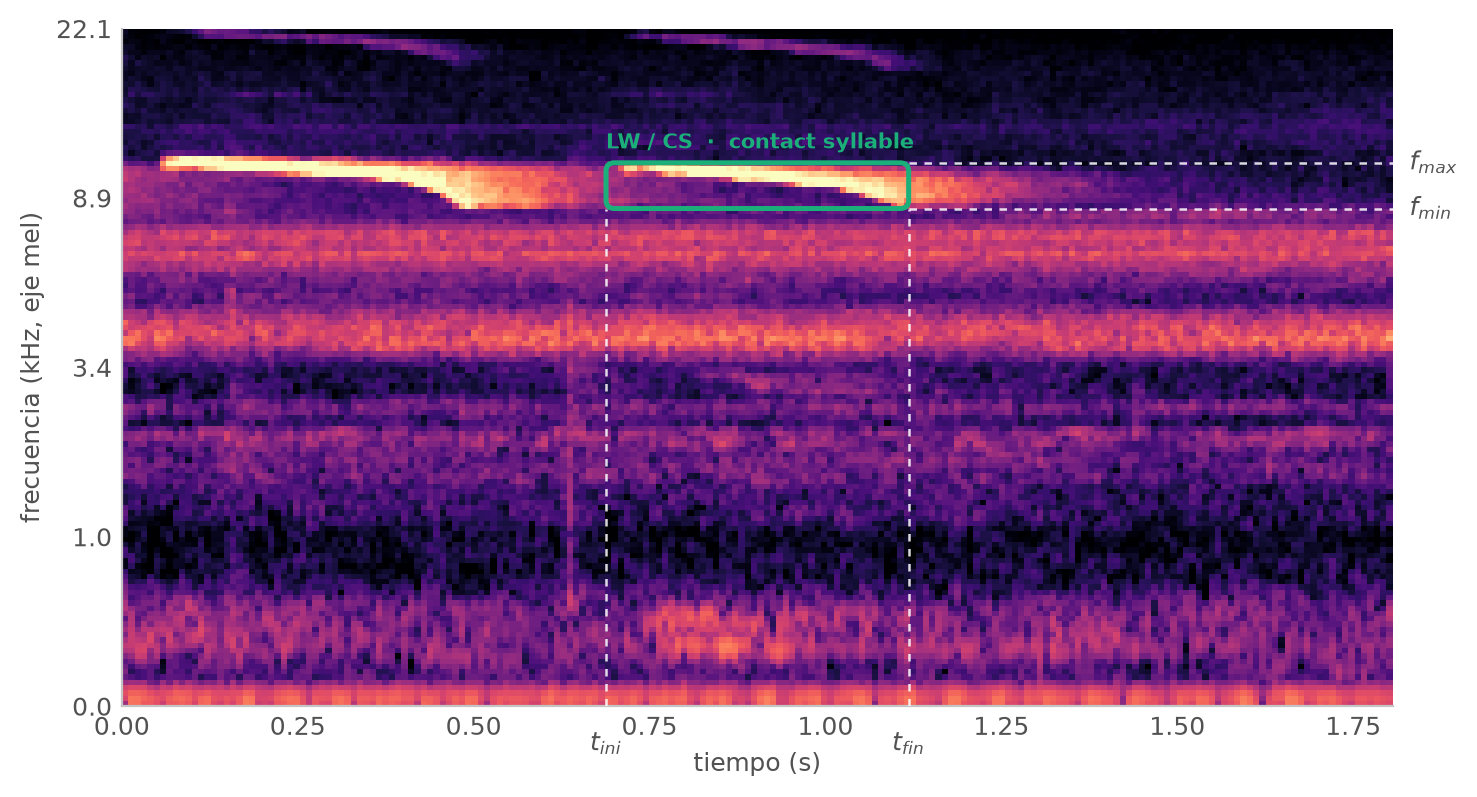
\includegraphics[width=0.85\textwidth]{figures/annotation_example.png}
    \caption{Ejemplo de anotación tiempo--frecuencia en Raven.}
    \label{fig:annotation-example}
\end{figure}

\begin{table}[htbp]
    \centering
    \caption{Resumen por especie}
    \label{tab:resumen-dataset}
    \small
    % Encabezado agrupado: los rótulos largos ("Duración anotada (h)")
    % obligaban a \scriptsize para que la tabla entrara en el ancho de
    % texto, y dejaban la tabla en un cuerpo distinto al del resto.
    \begin{tabular}{@{}L{6.2cm}rrrr@{}}
        \toprule
                                        & \multicolumn{2}{c}{\textbf{Total}} & \multicolumn{2}{c}{\textbf{Con anotaciones}}                                                   \\
        \cmidrule(lr){2-3}\cmidrule(lr){4-5}
        \textbf{Especie (código)}       & \textbf{N.\textsuperscript{o}}     & \textbf{Horas}                               & \textbf{N.\textsuperscript{o}} & \textbf{Horas} \\
        \midrule
        % Códigos verificados contra src/domain/species.py y contra la
        % Tabla 2.1 del marco conceptual: AA = Aotus azarae (mono
        % nocturno), AS = Alouatta sara (aullador), CC = Cebus cuscinus
        % (capuchino de cabeza chata). Los tres coinciden. No cambiar sin
        % actualizar también la Tabla 2.1 y el vocabulario del capítulo 4.
        Mono ardilla boliviano (SB)     & 290                                & 3,08                                         & 256                            & 2,79           \\
        Mono aullador (AS)              & 808                                & 7,57                                         & 779                            & 7,27           \\
        Capuchino de cabeza grande (SM) & 659                                & 6,13                                         & 582                            & 5,31           \\
        Mono nocturno (AA)              & 116                                & 1,10                                         & 83                             & 0,78           \\
        Mono araña peruano (AC)         & 561                                & 6,07                                         & 383                            & 3,62           \\
        Capuchino de cabeza chata (CC)  & 16                                 & 0,11                                         & 7                              & 0,04           \\
        Tití de Toppin (PT)             & 375                                & 3,35                                         & 320                            & 2,82           \\
        Tamarino de Weddell (LW)        & 530                                & 5,28                                         & 410                            & 3,71           \\
        \midrule
        \textbf{Total}                  & \textbf{3\,355}                    & \textbf{32,69}                               & \textbf{2\,820}                & \textbf{26,36} \\
        \bottomrule
    \end{tabular}
\end{table}

\subsection{Análisis lento e inconsistente}

El cuello de botella habitual es la falta de tiempo-persona de
analistas entrenados \citep{stowell_computational_2022}, y recolectar anotaciones es
el principal cuello de botella para construir estos métodos \citep{nguyen_assessing_2021}.
El trabajo se hace a mano. El analista abre cada grabación, inspecciona el
espectrograma, dibuja un recuadro alrededor de cada vocalización y le asigna una
etiqueta. En detección de eventos sonoros,
recolectar etiquetas fuertes a gran escala consume mucho tiempo, y en la mayoría
de los casos varios trabajadores se reparten las anotaciones para construir un
solo conjunto de datos \citep{koga_lead_2024}.

Ese reparto introduce un segundo problema ya que la anotación manual es subjetiva, y
resulta difícil cuantificar los sesgos ligados al nivel de conocimiento
del analista \citep{gibb_2018}; estudios recientes muestran que la tarea genera
errores específicos de cada anotador \citep{nguyen_assessing_2021}. Al comparar varios anotadores
sobre el mismo audio, las etiquetas fuertes presentan variaciones grandes tanto en el tipo de
evento como en los tiempos de inicio y fin, hasta el punto de que determinar una
etiqueta única resulta difícil \citep{koga_lead_2024}. En bioacústica marina,
\citet{leroy_reliability_2018} encontraron menos del 50\,\% de acuerdo entre dos
analistas, y también un acuerdo pobre de un mismo analista al anotar dos veces el
mismo segmento.

La variación temporal en las etiquetas fuertes es inevitable, y afecta tanto al
entrenamiento del modelo como a la evaluación de su desempeño
\citep{koga_lead_2024}. Esto significa que en en proyectos donde se aplica PAM,
una gran parte del audio queda sin anotar y las etiquetas anotadas son inconsistentes.

\subsection{Investigaciones anteriores}

Los sistemas más difundidos clasifican segmentos de duración fija. BirdNET
identifica cientos de especies de aves puntuando ventanas cortas de audio
\citep{kahl_birdnet_2021} y, en un caso más cercano al de esta tesis, HOWLish
detecta aullidos de lobo con una precisión de 0,006 bajo un desbalance extremo,
y aun así reduce unas 15 veces el tiempo del operador frente a anotar todo a mano
\citep{Campos_Krofel_Rio-Maior_Renna_2025}. Ese resultado es relevante porque
muestra que, cuando un humano revisa la salida, aceptar precisión baja a cambio
de recall alto es una estrategia válida. Su limitación es la forma del resultado:
una probabilidad por segmento, no un evento delimitado.

Una segunda línea sí devuelve eventos. Los \textit{sound event bounding boxes}
formalizan cada predicción como una cuádrupla de clase, tiempo de inicio, tiempo
de fin y una puntuación global de confianza \citep{ebbers_sound_2024}. Es un
evento con extensión propia, pero esa extensión existe solo sobre el eje
temporal.

La tercera línea trata el espectrograma como una imagen. La idea de partida es
que los eventos acústicos se manifiestan como patrones bidimensionales de tiempo
y frecuencia, con texturas y estructuras geométricas propias, análogos a los
objetos que aparecen en imágenes naturales \citep{pham_eventness_2018}. El
trabajo más cercano al de esta tesis es NBM, que publica anotaciones precisas de
tiempo y frecuencia recolectadas por decenas de aficionados a las aves en
Francia, junto con un modelo de detección de objetos de dos etapas adaptado a
datos de audio \citep{airale_nbm_2025}.

\begin{figure}[htbp]
    \centering
    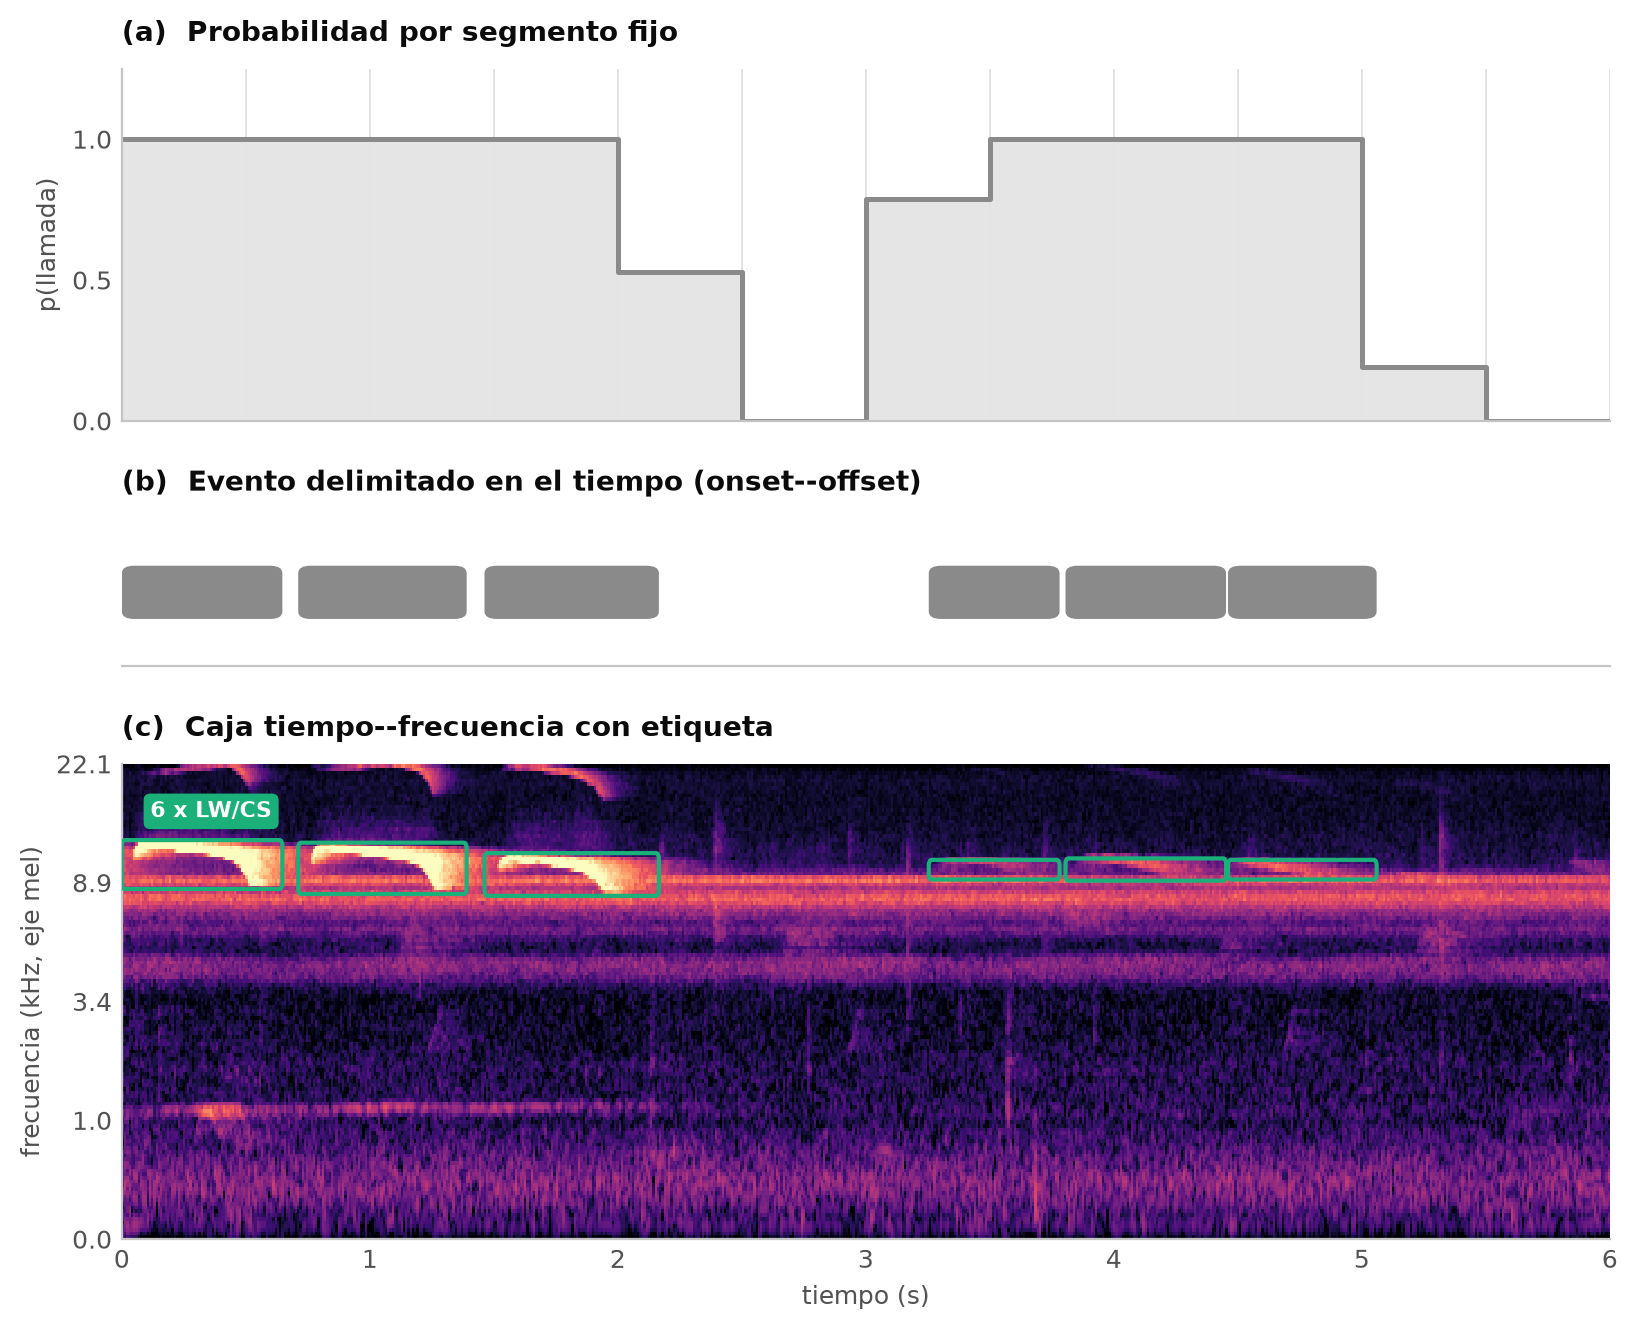
\includegraphics[width=\textwidth]{figures/output_forms.png}
    \caption{Tres formas de salida de un evento sonoro.}
    \label{fig:output-forms}
\end{figure}

\subsection{Vacío y contribución}
\label{sec:vacio}

El vacío tiene dos ejes, y esta tesis se sitúa en el cruce (Tabla~\ref{tab:vacio}).

\begin{table}[htbp]
    \centering
    \caption{Vacío del problema}
    \label{tab:vacio}
    \small
    % Columnas sin justificar y algo más anchas: justificadas a 3,6 cm
    % producían cortes forzados ("re-cursos", "mamí-feros") y huecos
    % entre palabras que se leían como desalineación.
    \begin{tabular}{@{}L{4.4cm}L{4.6cm}L{4.6cm}@{}}
        \toprule
                                                                                 & \thead[l]{Tarea madura:         \\ detección temporal}
                                                                                 & \thead[l]{Tarea poco explorada: \\ cajas tiempo--frecuencia} \\
        \midrule
        \textbf{Dominio con recursos}\newline (aves, mamíferos marinos, cánidos) &
        BirdNET, SEBB, YOHO                                                      &
        NBM \citep{airale_nbm_2025},
        YOLOv5 en focas barbudas \citep{escobar-amado_computer_2024}                                               \\
        \addlinespace
        \textbf{Dominio sin recursos}\newline (primates neotropicales)           &
        Heinicke et al. (2015), primates africanos                               &
        \textbf{Vacío: esta tesis}                                                                                 \\
        \bottomrule
    \end{tabular}
\end{table}

\rotulo{Eje de dominio.} Los sistemas maduros existen para aves, lobos y
mamíferos marinos. Para primates neotropicales de la Amazonía no hay un conjunto
público con anotaciones tiempo--frecuencia. La Tabla~\ref{tab:xenocanto} lo
documenta sobre el repositorio abierto de grabaciones de fauna más utilizado:
para las ocho especies objetivo, Xeno-canto contiene 32 grabaciones en primer
plano y poco más de una hora de audio en total, tres especies no tienen ninguna
grabación, y ninguna de las disponibles incluye anotaciones tiempo--frecuencia.

% TODO Añadir una segunda búsqueda documentada (Dryad, Zenodo o Macaulay
% Library) con la misma disciplina de término y fecha. Dos fuentes
% convergentes son mucho más difíciles de refutar que una sola.

\begin{table}[htbp]
    \centering
    \small
    % threeparttable: la nota al pie y el título toman el ancho real de
    % la tabla. Antes la nota iba en un minipage de 0,92\textwidth, más
    % ancho que la tabla, y quedaba descuadrada respecto de ella.
    \begin{threeparttable}
        \caption[Disponibilidad en Xeno-canto]{Disponibilidad de grabaciones de las especies objetivo en Xeno-canto}
        \label{tab:xenocanto}
        \begin{tabular}{@{}L{6.6cm}rr@{}}
            \toprule
            \textbf{Especie}                      & \thead{Grabaciones                  \\(primer plano)} & \thead{Duración\\total} \\
            \midrule
            \textit{Alouatta sara}                & 8                  & 41:14          \\
            \textit{Plecturocebus toppini}        & 13                 & 19:20          \\
            \textit{Ateles chamek}                & 4                  & 03:42          \\
            \textit{Saimiri boliviensis}          & 4                  & 02:28          \\
            \textit{Aotus azarae}                 & 3                  & 02:18          \\
            \textit{Cebus cuscinus}               & 0                  & N/D            \\
            \textit{Leontocebus weddelli}         & 0                  & N/D            \\
            \textit{Sapajus apella macrocephalus} & 0                  & N/D            \\
            \midrule
            \textbf{Total}                        & \textbf{32}        & \textbf{69:02} \\
            \bottomrule
        \end{tabular}
        \begin{tablenotes}[flushleft]
            \footnotesize
            \item Consulta realizada el 19 de agosto de 2026 sobre el nombre
            científico de cada especie \citep{Willem-Pier_Vellinga_2026}.
        \end{tablenotes}
    \end{threeparttable}
\end{table}

\rotulo{Eje de tarea.} El vacío tampoco es solo de dominio. La investigación
existente ha pasado por alto en gran medida el rango de frecuencia de los
eventos; el SED temporal descarta información codificada en el dominio
frecuencial, y por eso la detección precisa de cajas tiempo--frecuencia puede
asistir al investigador humano. Pese a esa relevancia, sigue siendo un área en
gran medida inexplorada \citep{zhu_sound_2025}.

En el cruce de ambos ejes se sitúa esta tesis, que desarrolla un protocolo de
curación y estandarización sobre las anotaciones producidas por el equipo de
investigación, y un detector que devuelve cajas tiempo--frecuencia con especie,
tipo de llamada y confianza, concebido como herramienta de pre-anotación
asistida.

\section{Árbol de problemas}

El árbol se estructura siguiendo el heurístico de análisis causa--efecto
propuesto por \citet{vesely_problem_2008}, y sirve de puente entre la brecha
operativa descrita en la sección anterior y los objetivos de la investigación.
Organiza el área temática en causas, problema central y efectos para ordenar el
trabajo posterior, sin cuantificar las relaciones entre sus elementos.

\begin{figure}[htbp]
    \centering
    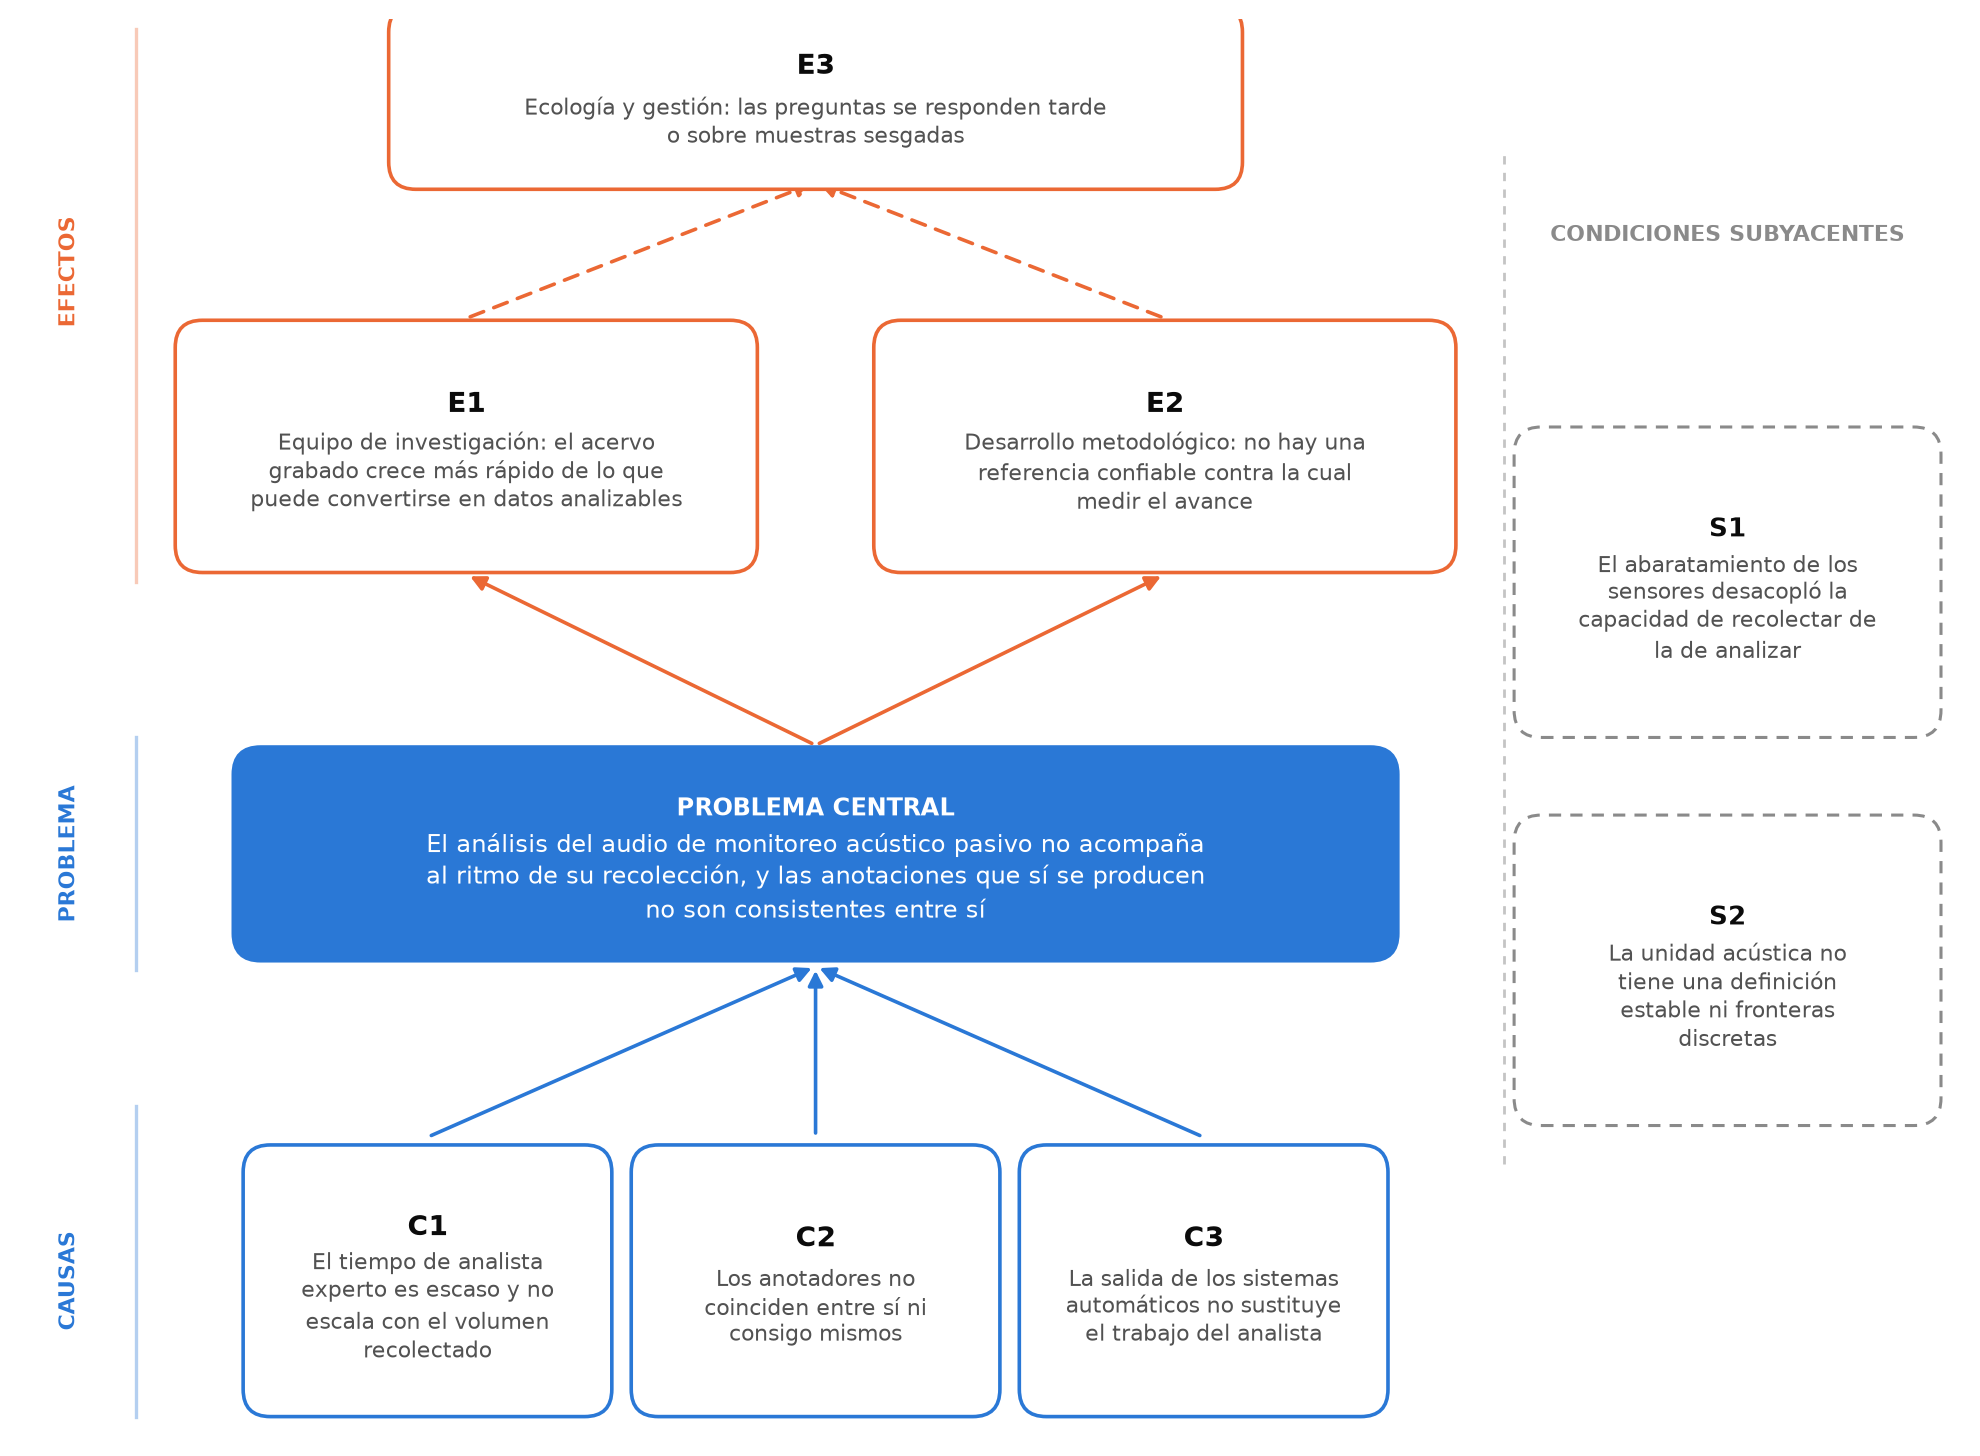
\includegraphics[width=\textwidth]{figures/problem_tree.png}
    \caption{Árbol de problemas.}
    \label{fig:problem-tree}
\end{figure}

\subsection{Condiciones subyacentes}

Dos condiciones enmarcan el problema sin ser causas sobre las que esta tesis
pueda actuar. Se consignan aparte, siguiendo la recomendación de
\citet{vesely_problem_2008} de ubicar fuera del eje causal aquello sin lo cual el
problema no existiría o existiría de otra forma.

\paragraph{S1: Grabar se volvió barato, pero analizar no}
Los sensores de bajo costo permiten desplegar redes de muchos micrófonos a
escala \citep{gibb_2018}. La condición no es negativa en sí misma; es la que
vuelve visible y creciente la distancia entre lo que se graba y lo que se llega
a revisar.

\paragraph{S2: La unidad acústica no tiene una definición estable ni fronteras
    discretas}
Las unidades acústicas pueden estar jerárquicamente anidadas, de modo
que una secuencia de unidades puede considerarse ella misma una unidad y ser
reemplazada por una etiqueta; se organizan en notas, trinos, sílabas, frases,
motivos y cantos, y las definiciones de unidad varían ampliamente entre
investigadores, incluso dentro de un mismo grupo taxonómico
\citep{kershenbaum_acoustic_2016}. A ello se suma que las unidades producidas por
animales exhiben variación graduada en sus rasgos, mientras que la mayoría de
métodos analíticos asume categorías discretas \citep{kershenbaum_acoustic_2016}.
La indefinición de granularidad es, entonces, anterior al anotador y no se
resuelve entrenándolo mejor. Esta condición es la que justifica, más adelante,
una curación metodológica explícita en lugar de una corrección de las anotaciones
recibidas.

\subsection{Problema central}

\begin{quote}
    El análisis del audio de monitoreo acústico pasivo no acompaña al ritmo de su
    recolección, y las anotaciones que sí se producen no son consistentes entre sí.
\end{quote}

El enunciado tiene deliberadamente dos predicados, porque el problema tiene dos
dimensiones que ninguna de las dos agota por separado: un déficit de
\emph{caudal} (se anota mucho menos de lo que se graba) y un déficit de
\emph{consistencia} (lo que se anota no obedece a un criterio único). Un
planteamiento que solo recogiera el primero dejaría sin cubrir la causa C2 y el
efecto E2; uno que solo recogiera el segundo no explicaría todo el audio que
queda sin anotar.

Del lado de la recolección, el despliegue a escala es hoy accesible (S1). Del
lado del análisis, la gran cantidad de audio que se acumula hace que un cuello de
botella común sea la falta de tiempo-persona de analistas entrenados
\citep{stowell_computational_2022}. Conforme escala el número de grabadoras
desplegadas, detectar señales acústicas en los paisajes sonoros registrados se
vuelve un obstáculo logístico que limita la escalabilidad de los estudios de PAM
\citep{Campos_Krofel_Rio-Maior_Renna_2025}.

% TODO EVIDENCIA LOCAL
% La figura de abajo aporta la mitad del dato que faltaba: horas
% recibidas, horas con archivo de anotación y minutos de evento
% anotado, por especie. Lo que sigue sin estar es la magnitud del
% acervo SIN revisar y las horas-analista disponibles por semana:
% esos dos números tiene que darlos el equipo, porque data/cleaned
% ya es el material curado que entregaron.
% ===================================================================

\begin{figure}[htbp]
    \centering
    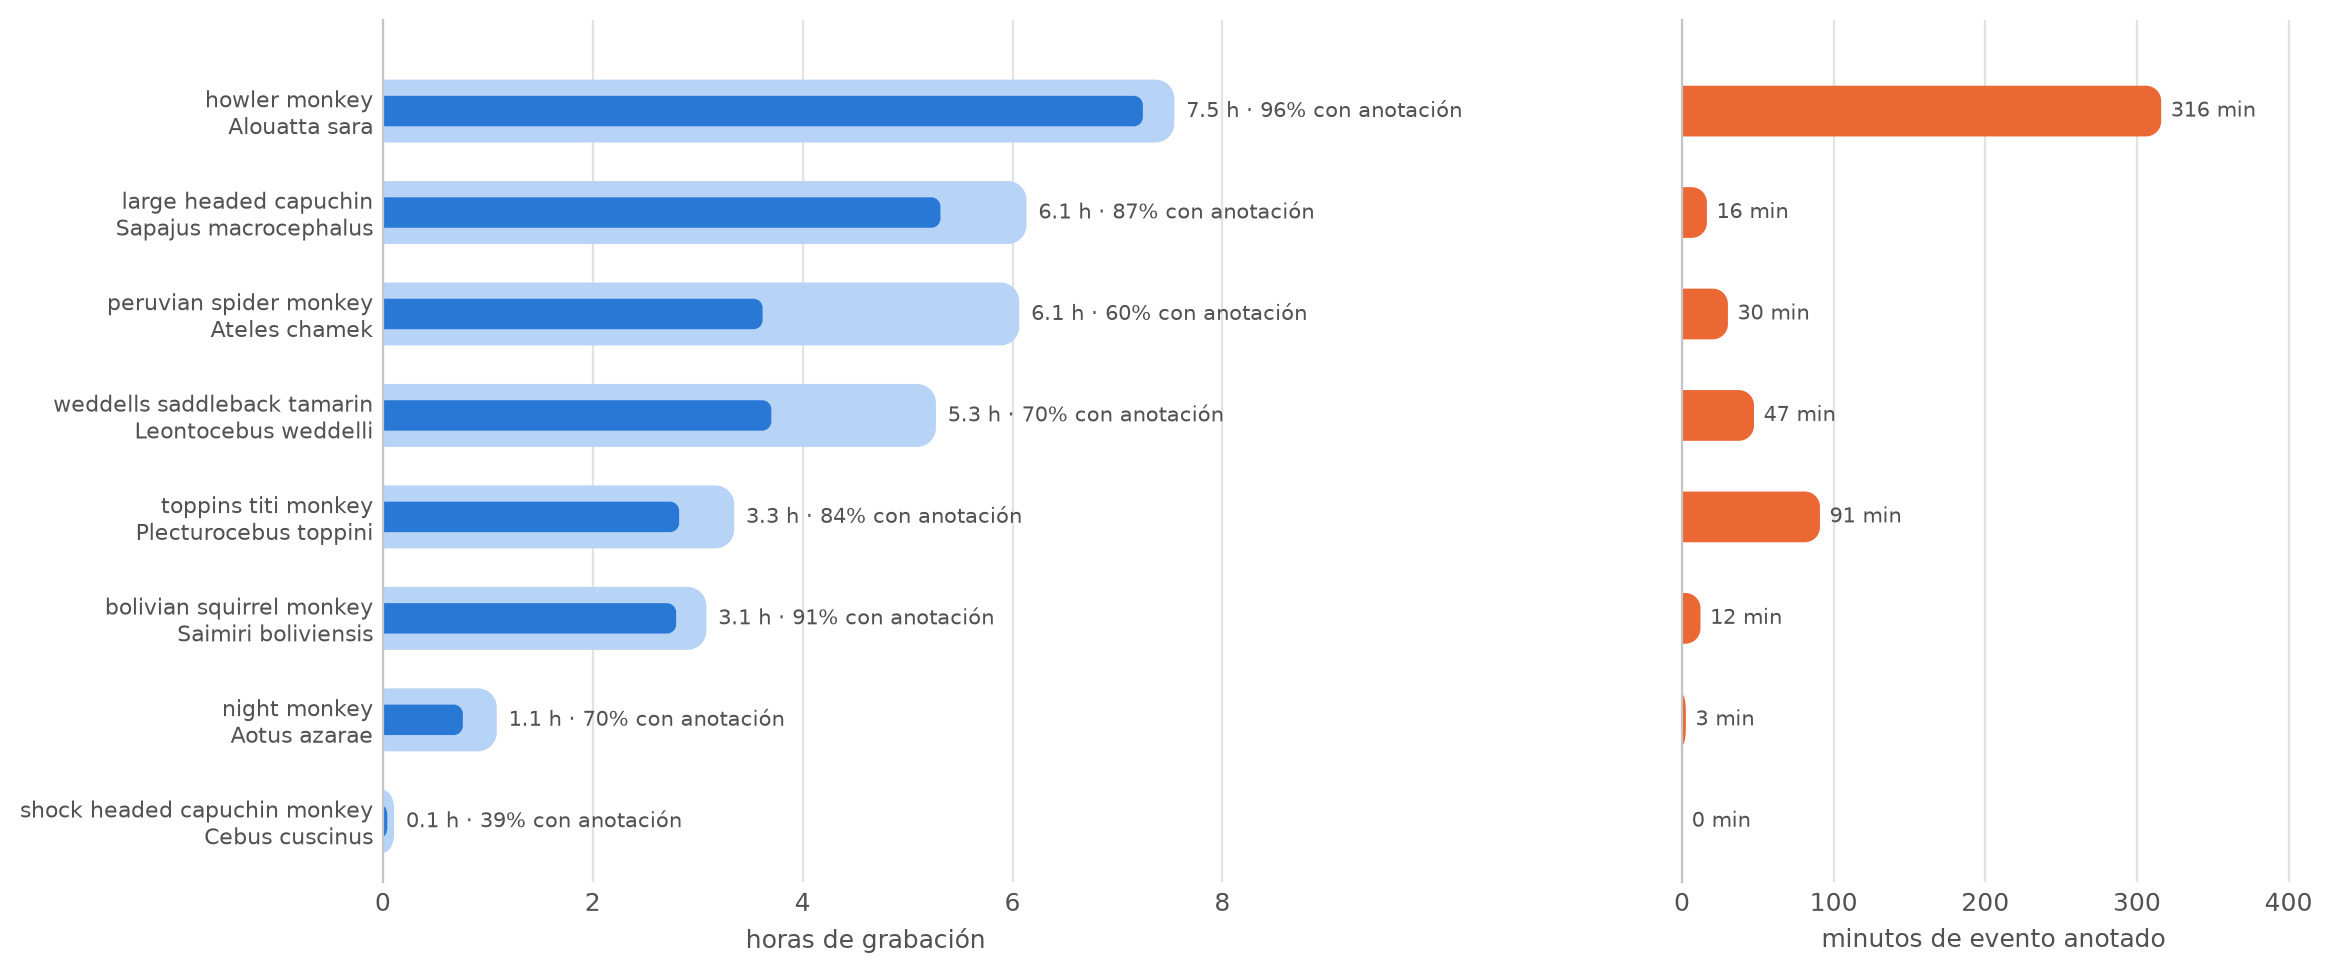
\includegraphics[width=\textwidth]{figures/recorded_vs_annotated.png}
    \caption{Material recibido por especie.}
    \label{fig:recorded-vs-annotated}
\end{figure}

\subsection{Causas}

\paragraph{C1: Hay pocas horas de analista experto disponibles}
Los eventos sonoros requieren que un experto los anote con las etiquetas
correctas, y ese tiempo experto suele escasear; la restricción se siente tanto en
distinciones categóricas finas como en el monitoreo a gran escala, donde el
volumen de datos excede con mucho las horas-persona disponibles
\citep{stowell_computational_2022}. En detección de eventos sonoros, recolectar
etiquetas fuertes a gran escala consume mucho tiempo, y por eso varios
trabajadores se reparten las anotaciones para construir un solo conjunto de datos
\citep{koga_lead_2024}. El reparto entre anotadores es la respuesta habitual a
esta restricción, y es también el punto donde C1 y C2 se encuentran: alivia el
caudal a costa de multiplicar los criterios en juego.

\paragraph{C2: Inconsistencia entre anotadores y dentro de un mismo anotador}
La tarea es subjetiva y genera errores específicos de cada anotador
\citep{nguyen_assessing_2021}, y los sesgos ligados al nivel de conocimiento del
analista son difíciles de cuantificar \citep{gibb_2018}. La magnitud
está medida: menos del 50\,\% de acuerdo entre analistas, y acuerdo pobre de un
mismo analista consigo mismo \citep{leroy_reliability_2018}; con 20 anotadores
por clip, las etiquetas fuertes presentan variaciones grandes en tipo de evento y
en tiempos de inicio y fin \citep{koga_lead_2024}. Estudios previos no han
encontrado soluciones suficientes, y la variación afecta tanto el entrenamiento
como la evaluación \citep{koga_lead_2024}.

Interesa subrayar que este desacuerdo es una propiedad medible de la tarea y no
un defecto individual corregible: descansa sobre S2, que fija su piso. Reducirlo
a cero no es un objetivo alcanzable, y cualquier propuesta metodológica debe
trabajar con él en lugar de suponerlo ausente.

\paragraph{C3: La salida de los sistemas automáticos no sustituye el trabajo
    del analista}
La automatización sería la vía natural para aliviar C1, pero su producto actual
no es un reemplazo directo del insumo que el analista necesita. Esto ocurre por
dos motivos distintos, uno de representación y otro de cobertura.

En cuanto a la representación, los sistemas basados en segmentos fijos entregan
una probabilidad asociada a una rejilla, no un evento con extensión propia:
BirdNET divide las grabaciones en fragmentos de 3\,s y almacena las
probabilidades por especie de cada segmento \citep{kahl_birdnet_2021}, y HOWLish
segmenta en ejemplos de 0,96\,s y promedia las predicciones con una ventana móvil
\citep{Campos_Krofel_Rio-Maior_Renna_2025}. Los sistemas que sí entregan eventos
delimitados los definen solo sobre el eje temporal, sea como cuádruplas de clase,
onset, offset y confianza \citep{ebbers_sound_2024}, sea regresando los puntos de
inicio y fin de cada clase \citep{venkatesh_you_2022}. La frecuencia, sin
embargo, aporta información que el biólogo usa: las cajas predichas llevan
información estadística embebida sobre la vocalización, como su duración, ancho de
banda y frecuencia central \citep{escobar-amado_computer_2024}.

En cuanto a la cobertura, aun cuando la precisión es alta, los métodos del estado
del arte fallan con regularidad al distinguir llamadas tenues, transitorias o
parcialmente enmascaradas, produciendo tasas altas de falsos negativos
\citep{gibb_2018}. Una salida automática incompleta no descarga al
analista: lo obliga a revisar igual.

\subsection{Efectos}

Los efectos se organizan por actor afectado, siguiendo el criterio que
\citet{vesely_problem_2008} ilustra en su tercer ejemplo, en lugar de asignar un
efecto a cada causa. E1 y E2 son efectos directos; E3 se deriva de ambos.

\paragraph{E1: Para el equipo de investigación, el material grabado crece más
    rápido de lo que puede analizarse}
El volumen de datos excede con mucho las horas-persona disponibles
\citep{stowell_computational_2022}, y la detección de señales en los paisajes
sonoros registrados se convierte en un obstáculo logístico conforme escalan
los despliegues \citep{Campos_Krofel_Rio-Maior_Renna_2025}. El efecto
práctico es que el esfuerzo y el gasto de despliegue quedan inmovilizados en
material sin procesar, y que la porción del material efectivamente anotada
responde a la disponibilidad del analista antes que a un criterio de muestreo.

\paragraph{E2: Para el desarrollo metodológico, no hay una referencia
    confiable contra la cual medir el avance}
La variación en las etiquetas fuertes no solo afecta el entrenamiento del
modelo, sino que tiene un impacto significativo sobre la evaluación de su
desempeño \citep{koga_lead_2024}. En el terreno de las cajas
tiempo--frecuencia, \citet{zhu_sound_2025} observan desplazamientos
relativamente grandes de las cajas predichas frente a las anotadas, y
concluyen que las fronteras de los eventos son borrosas y difíciles de
determinar, por lo que fijar un umbral de IoU bajo es razonable. A la
heterogeneidad se suma un faltante no aleatorio: las llamadas tenues o
enmascaradas escapan a los métodos automáticos \citep{gibb_2018}, de
modo que los eventos ausentes de la referencia son sistemáticamente los más
difíciles. La consecuencia es que las cifras de desempeño reportadas son
difíciles de comparar entre trabajos y tienden a describir mejor las
condiciones fáciles que el problema completo.

\paragraph{E3: Para la ecología y la gestión, las preguntas se responden
    tarde o sobre muestras sesgadas}
Efecto indirecto, derivado de E1 y E2. El PAM es cada vez más adecuado para
programas de monitoreo orientados a objetivos, cuyos protocolos deben ser
estandarizables, escalables y financieramente sostenibles
\citep{gibb_2018}; sus beneficios incluyen el muestreo continuo con
poco esfuerzo manual y una mayor probabilidad de detectar especies raras o
poco vocales \citep{gibb_2018}. Cuando el análisis no acompaña a la
recolección, esas ventajas no se materializan: la ventaja de detección de lo
raro se pierde por E1, y la confianza en lo que se reporta se erosiona por E2.
En primates, \citet{heinicke_2015} ya habían señalado el costo de
esta brecha al evaluar un sistema de monitoreo acústico en un ambiente de
selva altamente ruidoso.

% ===================================================================
\section{Objetivos}
% ===================================================================

\subsection{Objetivo general}

\begin{quote}
    \textbf{OG.} Desarrollar y evaluar un sistema de pre-anotación asistida 
    que proponga cajas tiempo--frecuencia con especie y tipo de llamada sobre 
    grabaciones de PAM de primates amazónicos, con el fin de maximizar la 
    cobertura de eventos anotados bajo una carga de revisión acotada.
\end{quote}

El encuadre asistido cuenta con respaldo en la literatura. La inteligencia
artificial no reemplaza la experiencia, y conforme estos sistemas se estandarizan
asumen el papel de pares expertos con quienes se consulta y debate, sin desplazar
el rol del experto ni el del trabajo colaborativo
\citep{stowell_computational_2022}. También tiene precedente cuantificado en
primates. \citet{heinicke_2015}
evaluaron un sistema de monitoreo acústico para cuatro especies de primates en el
ambiente altamente ruidoso del Parque Nacional Taï, y reportan que, pese a una
precisión aparentemente baja, la inversión de tiempo para remover manualmente los
falsos positivos de la salida del sistema fue de apenas 3--5\,\% comparada con la
de un humano recolectando y procesando los datos de vocalización.

% TODO VERIFICAR: confirmar que Heinicke et al. (2015) trabajan con primates
% africanos (Parque Nacional Taï, Costa de Marfil). Si es así, mantener la
% redacción como "cuatro especies de primates" sin insinuar que son
% neotropicales. El valor de la cita está en la TAREA, no en el taxón.

El mismo patrón se repite fuera de primates, y lo hace con una distinción que
este objetivo general adopta de forma deliberada. HOWLish recupera el 81,3\,\% de
los eventos de aullido observados y ofrece una reducción de 15 veces en el tiempo
del operador frente a la detección totalmente manual, y su tubería redujo 22
veces el volumen de datos que un operador debía procesar manualmente
\citep{Campos_Krofel_Rio-Maior_Renna_2025}. Son dos cifras de naturaleza
distinta: la primera es una medida de tiempo humano y exige cronometrar a una
persona; la segunda es una cantidad contable que se deriva de la propia salida
del sistema. Por eso el enunciado habla de \emph{carga} de revisión y no de
tiempo de revisión: la carga —cuántas propuestas hay que inspeccionar y cuánto
audio puede omitirse por completo— es la magnitud que este trabajo puede medir
sobre su propio conjunto de prueba, sin depender de la disponibilidad de un
revisor externo. El dato de \citet{heinicke_2015} conserva su lugar como
motivación, pues muestra que el encuadre asistido es rentable en primates y en
selva ruidosa, pero no como indicador.

El enunciado fija además el compromiso que el sistema asume de antemano:
priorizar la cobertura aceptando falsos positivos. Ese sesgo no es una concesión
sino una decisión con precedente cuantificado, ya que HOWLish resulta útil
operando con una precisión de 0,006 bajo desbalance extremo
\citep{Campos_Krofel_Rio-Maior_Renna_2025}. Su contrapartida es que la carga
generada por ese sesgo debe quedar acotada y reportada, y de eso se ocupa OE3.

\subsection{Objetivos específicos}

Cada objetivo específico responde a una de las tres causas del árbol: OE1 a la
inconsistencia del etiquetado (C2), OE2 a la forma de la salida (C3) y OE3 a la
escasez de horas de analista (C1).

\begin{description}
    \item[OE1.] Definir un protocolo de curación y estandarización, y aplicarlo
          sobre las anotaciones entregadas por el equipo de investigación para construir
          un conjunto de datos consistente de cajas tiempo--frecuencia etiquetadas por
          especie y tipo de llamada.

    \item[OE2.] Implementar y evaluar un detector que reciba un espectrograma y
          devuelva cajas tiempo--frecuencia con especie, tipo de llamada y confianza,
          comparándolo con una línea base establecida.

    \item[OE3.] Caracterizar el comportamiento operativo del detector sobre un conjunto 
          de prueba independiente, cuantificando la cobertura de las anotaciones de 
          referencia, la carga de revisión asociada y la naturaleza de sus discrepancias.
\end{description}

% ===================================================================
\section{Resultados esperados}
\label{sec:resultados}
% ===================================================================

\subsection{OE1: Protocolo y conjunto de datos curado}

Las grabaciones y las anotaciones primarias provienen del equipo de
investigación. La contribución de esta tesis es la normalización, el particionado
y la caracterización del conjunto derivado, no la anotación original.

\begin{table}[htbp]
    \centering
    \caption[IOV de OE1]{Resultados esperados, medios de verificación e indicadores objetivamente verificables de OE1}
    \label{tab:iov-oe1}
    \small
    \begin{tabular}{@{}L{1.0cm}L{3.7cm}L{3.2cm}L{6.1cm}@{}}
        \toprule
        \textbf{RE} & \textbf{Resultado} & \textbf{Medio de verificación} & \textbf{Indicador objetivamente verificable (IOV)} \\
        \midrule
        RE1.1 & Protocolo de curación y estandarización documentado. & Documento del protocolo. & Define la normalización de columnas y etiquetas, el mapa de sinónimos, el descarte de ruido y cajas degeneradas, la corrección de pares imposibles, el recorte al límite de Nyquist y el tratamiento de registros fuera de vocabulario. \\
        \addlinespace
        RE1.2 & Conjunto acústico curado y particionado para el experimento. & Directorio \texttt{data/processed/}: etiquetas, metadatos y tres archivos \texttt{.pt}. & Los archivos procesados cargan sin error; \texttt{meta.json} registra la semilla, el criterio de selección, las exclusiones, la etiqueta usada y la normalización; el código divide por archivo de grabación con proporciones 60/22,5/17,5 y no por ventanas aisladas. \\
        \addlinespace
        RE1.3 & Ficha del conjunto derivado. & Capítulo de curación, README y metadatos del conjunto. & Describe las ocho especies, el vocabulario, la composición, el desbalance, el diccionario de campos, el ventaneo de 3 s con salto de 1,5 s, la normalización log-mel, las exclusiones y las limitaciones conocidas. \\
        \bottomrule
    \end{tabular}
\end{table}

\begin{description}
    \item[RE1.1.] Protocolo documentado: vocabulario cerrado de clases, mapa de
          sinónimos, reglas de descarte y criterio de partición. Las definiciones de
          unidad y las etiquetas semánticas varían ampliamente entre investigadores
          \citep{kershenbaum_acoustic_2016}, lo que justifica cerrar el vocabulario, y
          los protocolos de monitoreo deben ser estandarizables
          \citep{gibb_2018}.

    \item[RE1.2.] Conjunto curado y particionado por archivo de grabación, sin
          solapamiento entre particiones. La variación en las etiquetas fuertes impacta
          la evaluación \citep{koga_lead_2024}, por lo que una partición que no infle
          artificialmente el resultado es condición para que las cifras sean
          interpretables.

    \item[RE1.3.] Ficha del conjunto derivado: composición, desbalance, sesgos
          conocidos y limitaciones. Pese a la importancia de los datos para el
          aprendizaje automático, no existe un proceso estandarizado para documentar
          conjuntos de datos; las \textit{datasheets} proponen documentar motivación,
          composición, proceso de recolección y usos recomendados, con el potencial de
          aumentar la transparencia y la rendición de cuentas
          \citep{gebru_2021}. La ficha distingue dos capas: el conjunto
          primario, producido por el equipo de investigación, y el conjunto derivado,
          producido por esta tesis.
\end{description}

La decisión de excluir las clases de frase se apoya directamente en
\citet{kershenbaum_acoustic_2016}: las unidades pueden estar jerárquicamente
anidadas, de modo que una secuencia de unidades puede considerarse ella misma una
unidad, y un detector de conjunto plano no puede representar esa relación.

% FIGURA 1.4 RESUELTA
% El diagrama del anidamiento frase -> sílaba existe como
% figures/nesting_phrase.png, sobre una grabación real, y está
% colocado en el capítulo 4 (sección \ref{sec:silabas}), junto al
% texto que ya lo explica. Desde aquí basta con referenciarlo.
% ===================================================================

\subsection{OE2: Detector y evaluación}

\begin{table}[htbp]
    \centering
    \caption[IOV de OE2]{Resultados esperados, medios de verificación e indicadores objetivamente verificables de OE2}
    \label{tab:iov-oe2}
    \small
    \begin{tabular}{@{}L{1.0cm}L{3.7cm}L{3.2cm}L{6.1cm}@{}}
        \toprule
        \textbf{RE} & \textbf{Resultado} & \textbf{Medio de verificación} & \textbf{Indicador objetivamente verificable (IOV)} \\
        \midrule
        RE2.1 & Diseño experimental, arquitectura propuesta y línea base. & Documento de diseño y módulo de arquitecturas. & Especifica la arquitectura AST-Deformable-DETR implementada, con dimensión 128, 64 consultas y 3 niveles, sus hiperparámetros, y define la comparación con las líneas base declaradas. \\
        \addlinespace
        RE2.2 & Pipeline reproducible de entrenamiento, evaluación e inferencia. & Scripts de datos, entrenamiento, evaluación e inferencia; módulos de \texttt{src/pipelines/}; \texttt{pyproject.toml} y manual técnico. & El pipeline genera los splits procesados, entrena desde un conjunto de configuración, evalúa un checkpoint y ejecuta inferencia sobre un WAV; las dependencias y comandos de ejecución están declarados. \\
        \addlinespace
        RE2.3 & Informe comparativo de resultados. & Informe de experimentación y archivos de métricas. & Reporta, como mínimo, recall, precisión, F1, IoU medio, AP a IoU 0,25 y 0,5, recall por clase y matriz de confusión; separa detección, encuadre y clasificación y justifica la selección del modelo. \\
        \addlinespace
        RE2.4 & Modelo final cargable y demostración funcional. & Checkpoint \texttt{.pth}, \texttt{labels.json} y ejecución de \texttt{src/infer.py}. & El checkpoint se carga sin claves incompatibles y la inferencia sobre un WAV produce un archivo tabulado con las columnas de Raven, incluidas coordenadas tiempo--frecuencia, especie, tipo de llamada y puntuación. \\
        \addlinespace
        RE2.5 & Código y modelo disponibles en un repositorio. & Repositorio de control de versiones. & La URL del repositorio permite localizar el código de curación, entrenamiento, evaluación e inferencia, junto con las instrucciones de ejecución y los artefactos del modelo final que se hayan decidido publicar. \\
        \bottomrule
    \end{tabular}
\end{table}

\begin{description}
    \item[RE2.1.] Documento de diseño: arquitectura propuesta y línea base, con
          justificación de ambas. Los eventos se manifiestan como patrones
          bidimensionales con texturas y estructuras geométricas propias, análogos a los
          objetos de imágenes naturales \citep{pham_eventness_2018}, y detectar un
          objeto implica tanto afirmar que una clase está presente como localizarla,
          localización que se representa típicamente mediante una caja delimitadora
          \citep{lin_2014}. La brecha de modalidad entre imagen y audio
          justifica sustituir los \textit{backbones} preentrenados en imágenes
          \citep{zhu_sound_2025}. Como precedentes de detección bidimensional en
          bioacústica se consideran \citet{escobar-amado_computer_2024} y
          \citet{airale_nbm_2025}, y como línea base sobre espectrogramas,
          \citet{gonzalez_yolo-based_2025}.

    \item[RE2.2.] Pipeline reproducible de entrenamiento, evaluación e
          inferencia. La pirámide multiescala corrige que las arquitecturas de tipo ViT
          y AST produzcan representaciones de escala única \citep{zhu_sound_2025}.

    \item[RE2.3.] Informe de evaluación desagregado en detección, encuadre y
          clasificación, con comparación contra la línea base. Un umbral de IoU bajo es
          razonable cuando las fronteras de los eventos son borrosas
          \citep{zhu_sound_2025}, y el sesgo hacia el recall se justifica por el fallo
          sistemático de los métodos automáticos ante llamadas tenues o enmascaradas
          \citep{gibb_2018}.

          % TODO PENDIENTE DE CITA
          % Falta la referencia que sostenga "AP a un umbral de IoU" como
          % métrica. La cita de Lin et al. (2014) que tienes extraída sostiene
          % la CAJA como representación (por eso está en RE2.1), no el
          % protocolo de evaluación. Busca el fragmento de la sección
          % "Evaluation" de COCO, o sustituye por Mesaros et al. (2021) para
          % el marco de métricas de SED.
          % =================================================================

    \item[RE2.4.] Modelo final y exportador a tabla de selección de Raven. Las
          cajas llevan información estadística embebida útil para el analista, como la
          duración, el ancho de banda y la frecuencia central
          \citep{escobar-amado_computer_2024}.

    \item[RE2.5.] Repositorio público con código y pesos del modelo.
\end{description}

El contraste que sostiene RE2.4 es directo: BirdNET y HOWLish entregan
probabilidad por segmento \citep{kahl_birdnet_2021,Campos_Krofel_Rio-Maior_Renna_2025},
los \textit{sound event bounding boxes} y YOHO entregan límites temporales
\citep{ebbers_sound_2024,venkatesh_you_2022}, y esta tesis entrega la tupla
completa de tiempo, frecuencia, especie, tipo de llamada y confianza.

\subsection{OE3: Cobertura, carga de revisión y análisis de discrepancias}

\begin{table}[htbp]
    \centering
    \caption[IOV de OE3]{Resultados esperados, medios de verificación e indicadores objetivamente verificables de OE3}
    \label{tab:iov-oe3}
    \small
    \begin{tabular}{@{}L{1.0cm}L{3.7cm}L{3.2cm}L{6.1cm}@{}}
        \toprule
        \textbf{RE} & \textbf{Resultado} & \textbf{Medio de verificación} & \textbf{Indicador objetivamente verificable (IOV)} \\
        \midrule
        RE3.1 & Protocolo de evaluación operativa. & Documento del protocolo, fechado antes de ejecutar la evaluación. & Especifica el subconjunto de prueba particionado por archivo y sin solapamiento, el punto de operación y el criterio con que se elige, el umbral IoU 0,5 de emparejamiento, la supresión de no máximos entre ventanas, el procedimiento de agregación por archivo y las cuatro categorías de la taxonomía de discrepancias. \\
        \addlinespace
        RE3.2 & Curva de cobertura frente a carga de revisión. & Informe de evaluación operativa, archivos de métricas y medición de inferencia. & Reporta la curva completa de cobertura (\textit{recall} por evento a IoU 0,5) frente a propuestas por hora de audio; el punto de operación elegido junto con su criterio; el cociente FP/TP; la fracción de audio sin ninguna propuesta como reducción de volumen; y el costo de inferencia en minutos de GPU por hora de audio. No fija un porcentaje de ahorro antes de medirlo. \\
        \addlinespace
        RE3.3 & Taxonomía geométrica de discrepancias. & Informe de análisis, tablas de distribución y panel de espectrogramas. & Distribuye las predicciones de alta confianza entre las cuatro categorías de la Tabla~\ref{tab:taxonomia-fp}; caracteriza la categoría D por banda de frecuencia, duración y puntuación frente a la distribución de los eventos anotados de cada clase; e incluye ejemplos visuales representativos de cada categoría sobre el espectrograma. \\
        \addlinespace
        RE3.4 & Validación experta de la categoría abierta \textit{(condicional)}. & Informe de validación, sujeto a la disponibilidad del equipo de investigación. & Si se concreta: resuelve una muestra de predicciones de categoría D entre evento omitido por la referencia y falso positivo genuino, y estima el acuerdo entre el modelo y el criterio experto. Su ausencia no compromete el cumplimiento de OE3. \\
        \bottomrule
    \end{tabular}
\end{table}

OE3 mide la utilidad operativa del sistema con magnitudes que se calculan sobre
el propio conjunto de prueba. Ninguno de sus tres resultados comprometidos
depende de cronometrar a un revisor externo, y el cuarto se declara condicional
justamente porque sí depende de él.

\begin{description}
    \item[RE3.1.] Protocolo de evaluación operativa, redactado y fechado antes de
          ejecutar la evaluación: material de prueba, punto de operación y criterio
          con que se elige, umbral de emparejamiento, supresión de no máximos entre
          ventanas, agregación por archivo y taxonomía de discrepancias, siguiendo el
          marco de tubería para identificación automatizada de sonidos
          \citep{gibb_2018}. Fijarlo de antemano impide elegir a posteriori el umbral
          o la métrica que mejor favorezcan al resultado ya obtenido.

    \item[RE3.2.] Curva de cobertura frente a carga de revisión, en lugar de una
          única cifra cronometrada. La curva expresa qué fracción de las anotaciones
          de referencia recupera el sistema en función de cuántas propuestas por hora
          de audio se pide inspeccionar, y sobre ella se elige el punto de operación:
          el umbral que maximiza la cobertura sujeto a un techo de propuestas por
          hora. El punto de operación deja así de ser una constante heredada y pasa a
          ser una decisión justificada. Las cinco magnitudes que se reportan
          —cobertura, propuestas por hora, FP/TP, reducción de volumen y costo de
          inferencia— se computan íntegramente sobre la partición de prueba. El
          precedente metodológico directo es la reducción de 22 veces en el volumen de
          datos que un operador debía procesar manualmente
          \citep{Campos_Krofel_Rio-Maior_Renna_2025}, indicador que ese trabajo deriva
          de la salida del sistema y no de un cronómetro; el mismo trabajo sostiene el
          compromiso de cobertura sobre precisión al resultar útil operando con una
          precisión de 0,006 bajo desbalance extremo. El dato de tiempo de
          \citet{heinicke_2015} queda como motivación del encuadre asistido, no como
          indicador de este resultado.

          Si el calendario lo permite, se añade una medición cronometrada sobre una
          muestra pequeña revisada por el propio autor, declarada de forma explícita
          como cota ilustrativa y no como validación experta.

    \item[RE3.3.] Taxonomía geométrica de las discrepancias entre las predicciones
          de alta confianza y las anotaciones de referencia, según la
          Tabla~\ref{tab:taxonomia-fp}. Las tres primeras categorías se resuelven sin
          consultar a nadie, porque quedan determinadas por la relación geométrica
          entre la caja predicha y una caja anotada que sí existe: son modos de error
          del modelo operando sobre eventos presentes en la referencia. Los dos que
          documenta \citet{zhu_sound_2025} —una caja anotada detectada como varias, y
          varias detectadas como una— corresponden a la categoría B, y la borrosidad
          de las fronteras del evento que ese mismo trabajo describe es lo que hace
          necesaria la categoría A.

          Solo la categoría D queda abierta, y se caracteriza estadísticamente en
          lugar de dejarse sin resolver: se compara la distribución de banda de
          frecuencia, duración y puntuación de esas predicciones contra la de los
          eventos anotados de cada clase. Si se parecen geométricamente a los eventos
          anotados y se concentran en las bandas correctas, eso constituye un
          \emph{indicio} —no una prueba— de que la referencia omite eventos. Que tal
          indicio sea plausible tiene respaldo: los métodos automáticos fallan con
          llamadas tenues o enmascaradas \citep{gibb_2018}, lo que implica la
          existencia de eventos válidos fuera del \textit{ground truth}, y la
          variabilidad intra-analista \citep{leroy_reliability_2018} apunta en la
          misma dirección desde el lado humano.

    \item[RE3.4.] Validación experta de una muestra de predicciones de categoría D,
          para resolver si son eventos omitidos por la referencia o falsos positivos
          genuinos, y estimar el acuerdo entre el modelo y el criterio experto. Se
          declara \textbf{condicional}, sujeto a la disponibilidad del equipo de
          investigación. Su función en el documento es doble: proteger el cierre de la
          tesis, que no queda supeditado a la agenda de un tercero, y dejar preparado
          el resultado adicional si esa disponibilidad se concreta.
\end{description}

\begin{table}[htbp]
    \centering
    \caption[Taxonomía de discrepancias]{Taxonomía geométrica de las discrepancias de alta confianza}
    \label{tab:taxonomia-fp}
    \small
    \begin{tabular}{@{}L{1.0cm}L{2.9cm}L{6.9cm}L{2.8cm}@{}}
        \toprule
        \textbf{Tipo} & \textbf{Discrepancia} & \textbf{Definición} & \textbf{¿Resoluble sin experto?} \\
        \midrule
        A & Encuadre  & Solapa con una anotación de la misma clase, pero con IoU inferior al umbral de emparejamiento.                       & Sí \\
        \addlinespace
        B & Unidad    & Varias predicciones sobre una misma anotación, o una predicción sobre varias anotaciones: división y fusión.          & Sí \\
        \addlinespace
        C & Clase     & Encuadre correcto sobre una anotación, con etiqueta de especie o de tipo de llamada incorrecta.                       & Sí \\
        \addlinespace
        D & Región sin anotación & No solapa con ninguna caja anotada. Puede ser un evento omitido por la referencia o un falso positivo genuino. & \textbf{No} \\
        \bottomrule
    \end{tabular}
\end{table}

\rotulo{Limitación declarada.} Sin revisión experta, las predicciones de alta
confianza situadas en regiones sin anotación (tipo D) no pueden clasificarse de
forma concluyente entre eventos omitidos por la referencia y falsos positivos
genuinos. Esta tesis las caracteriza geométricamente y las reporta como una
cantidad acotada, dejando su resolución como trabajo futuro condicionado a la
disponibilidad del equipo de investigación.

% ===================================================================
\section{Trazabilidad}
% ===================================================================

La relación entre las causas del problema, sus efectos y los productos
comprometidos se resume en la Tabla~\ref{tab:trazabilidad}. En la práctica, OE1
aborda la heterogeneidad del etiquetado, OE2 la representación funcional de los
eventos, y OE3 la utilidad operativa del sistema dentro del flujo de trabajo del
analista. OE3 sigue atacando C1, la escasez de horas de analista, pero lo hace
midiendo cuánto trabajo se evita y no cuánto tiempo tarda alguien en hacerlo.

\begin{table}[htbp]
    \centering
    \caption[Trazabilidad del planteamiento]{Trazabilidad entre causas, efectos, objetivos y resultados esperados}
    \label{tab:trazabilidad}
    \small
    \begin{tabular}{@{}L{3.6cm}L{2.0cm}L{2.0cm}L{6.0cm}@{}}
        \toprule
        \textbf{Causa}         & \textbf{Efecto} & \textbf{Objetivo} & \textbf{Resultados esperados}               \\
        \midrule
        C1: Velocidad          & E1              & OE3               & RE3.1, RE3.2, RE3.3 y RE3.4 (condicional)   \\
        \addlinespace
        C2: Consistencia       & E2              & OE1               & RE1.1, RE1.2, RE1.3                         \\
        \addlinespace
        C3: Forma de la salida & E1, E2          & OE2               & RE2.1, RE2.2, RE2.3, RE2.4, RE2.5           \\
        \midrule
        E1, E2                 & E3              & OG                & Sistema de pre-anotación asistida integrado \\
        \bottomrule
    \end{tabular}
\end{table}

% ===================================================================
\section{Métodos y procedimientos}
\label{sec:metodos}
% ===================================================================

\subsection{Metodología CRISP-DM}

El desarrollo se organiza siguiendo CRISP-DM (\textit{Cross-Industry Standard
    Process for Data Mining}), un marco iterativo, independiente de la industria y
de la herramienta, que proporciona una hoja de ruta general para proyectos de
minería de datos \citep{chapman_crisp-dm_2000}. Su estructura cíclica, desde la
comprensión del problema hasta el despliegue de la solución, se ajusta a un proyecto
de investigación aplicada en el que la comprensión de los datos, la
experimentación con modelos y la evaluación continua se realimentan entre sí.
La Tabla~\ref{tab:crispdm} resume la correspondencia entre las seis fases, los
objetivos específicos y los capítulos de este documento.

\begin{table}[htbp]
    \centering
    \caption{Fases de CRISP-DM y objetivos}
    \label{tab:crispdm}
    \small
    \begin{tabular}{@{}L{4.6cm}L{5.9cm}L{1.8cm}L{1.9cm}@{}}
        \toprule
        \textbf{Fase}               & \textbf{Contenido en este proyecto}                                          & \textbf{Objetivo} & \textbf{Capítulo} \\
        \midrule
        1. Comprensión del negocio  & Árbol de problemas, objetivos y criterios de éxito                           & N/A               & 1                 \\
        \addlinespace
        2. Comprensión de los datos & Análisis exploratorio y verificación de calidad de las anotaciones recibidas & OE1               & 4                 \\
        \addlinespace
        3. Preparación de datos     & Curación, vocabulario cerrado, particionado y ventaneo                       & OE1               & 4                 \\
        \addlinespace
        4. Modelado                 & Detector de cajas tiempo--frecuencia y línea base                            & OE2               & 5                 \\
        \addlinespace
        5. Evaluación               & Métricas por eje, discrepancias y carga de revisión                          & OE2, OE3          & 5                 \\
        \addlinespace
        6. Despliegue               & Inferencia por lotes y exportación a tabla de selección de Raven             & OE2               & 5                 \\
        \bottomrule
    \end{tabular}
\end{table}

\begin{figure}[tb]
    \centering
    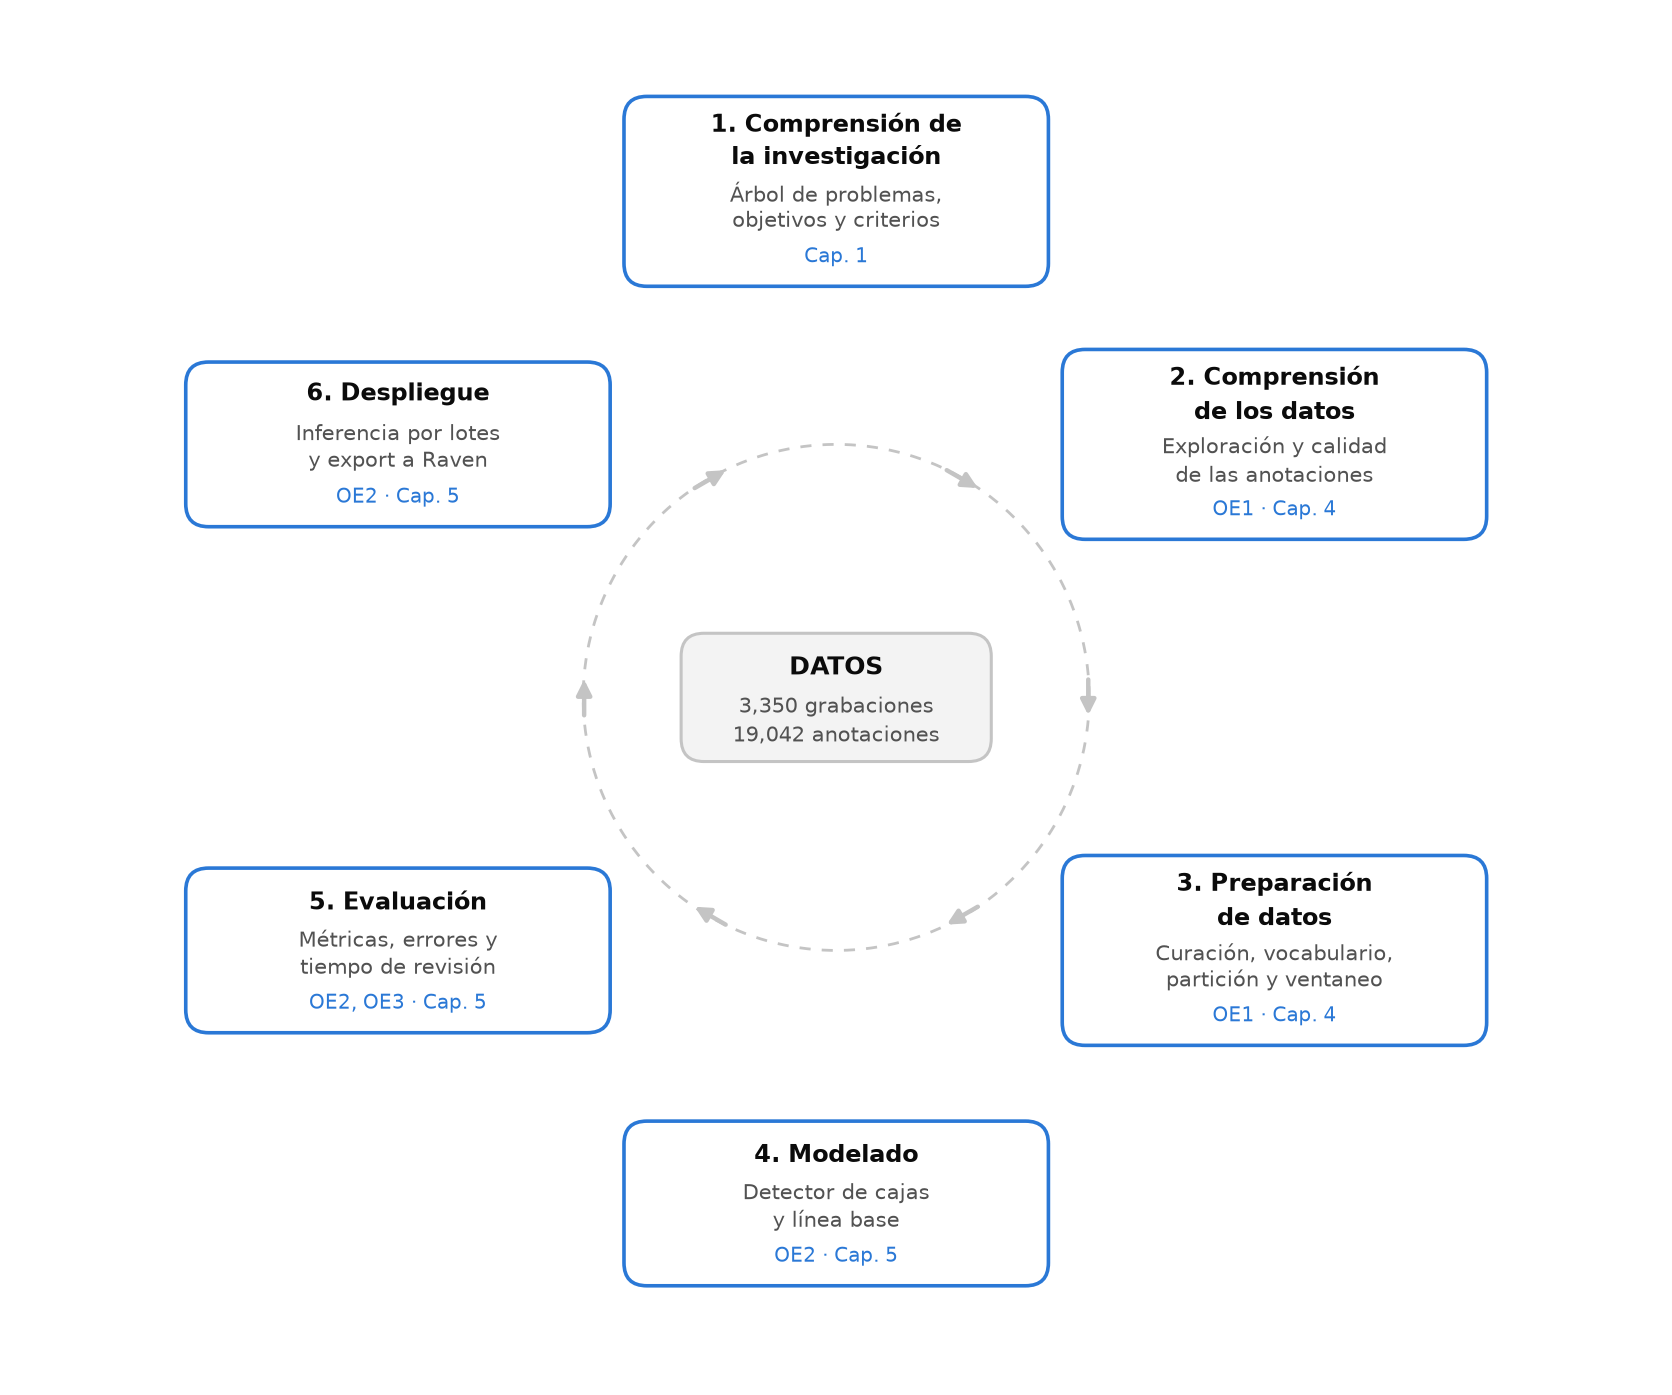
\includegraphics[width=0.58\textwidth]{figures/crisp_dm.png}
    \caption{Fases de CRISP-DM del proyecto.}
    \label{fig:crisp-dm}
\end{figure}

\paragraph{Fase 1: Comprensión del negocio o de la investigación.}
Convierte el conocimiento del dominio y los objetivos del proyecto en una
definición formal del problema de minería de datos
\citep{chapman_crisp-dm_2000}. Esa traducción es el contenido de las secciones
anteriores de este capítulo: la brecha operativa se estructura como árbol de
problemas y de ahí derivan el objetivo general, los objetivos específicos y los
resultados esperados. Los criterios de éxito son a la vez técnicos, relacionados
con el desempeño en detección, encuadre y clasificación, y operativos, vinculados
con la cobertura alcanzada y con la carga de revisión que genera alcanzarla, como
recomienda el marco para asegurar que el resultado sea útil y no solo correcto.

\paragraph{Fase 2: Comprensión de los datos.}
Los datos primarios son grabaciones en formato WAV muestreadas a 44,1\,kHz,
capturadas con dispositivos AudioMoth y entregadas por el equipo de
investigación junto con sus anotaciones. Cada especie llega en una carpeta con
grabaciones de duración heterogénea y un archivo de texto delimitado por
tabulaciones producido con Raven Pro, en el que cada fila registra tiempo de
inicio y fin, frecuencia mínima y máxima, amplitud, calidad, etiqueta de especie
y etiqueta de tipo de llamada. La fase comprende el análisis exploratorio
visualización de espectrogramas, distribución de clases, distribución de
duraciones y rangos de frecuencia, junto con la verificación de calidad de los
archivos de audio corruptos, errores tipográficos y etiquetas inconsistentes. El
Capítulo~\ref{cap:curacion} desarrolla ambos.

\paragraph{Fase 3: Preparación de datos.}
Comprende la limpieza y normalización de etiquetas sobre un vocabulario cerrado,
el preprocesamiento del audio, el cálculo de la representación
tiempo--frecuencia, la segmentación de las grabaciones largas en ventanas de
duración fija con solapamiento, y el aumento de datos mediante adición de ruido de
fondo del propio entorno, desplazamiento de tono, estiramiento temporal y
enmascaramiento de bloques de tiempo o frecuencia sobre el espectrograma.
Aquí se resuelve la comparación entre log-mel y PCEN anunciada en la
sección~\ref{sec:representacion}, bajo el criterio allí declarado.

\paragraph{Fase 4: Modelado.}
La forma de la salida no está en discusión: el sistema debe emitir la tupla
completa de la ecuación~\eqref{eq:tupla}, y esa exigencia excluye de antemano
toda arquitectura cuya cabeza produzca una probabilidad por trama o por segmento.
Lo que se compara, por tanto, no son familias de arquitectura sino
configuraciones que sí satisfacen la exigencia: la arquitectura propuesta sobre
un extractor de audio con cabeza de detección, en sus dos pasos temporales, y dos
líneas base de detector sobre espectrogramas, un detector de una etapa
\citep{gonzalez_yolo-based_2025} y uno de dos etapas con propuestas de región.

La regla de decisión se fija antes de entrenar: gana la configuración con mayor
valor de la métrica principal definida en la Fase~5, medida sobre la partición de
\emph{validación}; la partición de prueba se reserva para reportar el desempeño
de la configuración ya elegida y no participa de la elección. La implementación
se realiza en PyTorch con código modular, separando la definición de la
arquitectura, el bucle de entrenamiento y las utilidades.

\paragraph{Fase 5: Evaluación.}
\label{sec:metricas}
Los modelos entrenados se evalúan sobre la partición de prueba y los resultados
se leen contra los criterios de éxito de la Fase~1. El análisis no se agota en
una cifra agregada: identifica qué clases se detectan mejor y peor, qué tipos de
error predominan, entre ellos la confusión entre especies acústicamente próximas,
los falsos positivos por ruido y los errores de localización en tiempo o en frecuencia, y
acompaña las cifras con ejemplos visualizados sobre el espectrograma.

Reportar varias métricas sin jerarquía permitiría elegir a posteriori la que
favorezca al modelo preferido.
Para evitarlo, la Tabla~\ref{tab:metricas-sed} asigna a cada una un rol fijado de
antemano.

La \textbf{métrica principal} es el \textit{recall} a nivel de evento
\emph{agnóstico a la clase}, con un umbral de IoU bidimensional de 0,5 y un
umbral de confianza de 0,5. Que sea agnóstico a la clase no es un descuido: la
sección~\ref{sec:geometria} muestra que la geometría separa especies pero no
tipos de llamada dentro de una misma especie, de modo que localizar y etiquetar
son problemas de dificultad distinta, y mezclarlos en una sola cifra oculta cuál
de los dos falla. El \textit{recall} manda porque el sistema es de pre-anotación
asistida y un humano revisa su salida.

El \textbf{criterio de selección de \textit{checkpoint}} es una F-$\beta$ con
$\beta = 3$, que pondera el \textit{recall} nueve veces más que la precisión, y
es la traducción operativa del requisito enunciado con el objetivo general:
perder una vocalización cuesta más que revisar un falso positivo. Para que ese
sesgo no degenere en proponer indiscriminadamente, junto a él se reporta el
cociente \textbf{FP/TP al punto de operación}, que es literalmente la carga de
revisión que el experto asume por cada acierto y la magnitud que conecta esta
fase con OE3.

El umbral de confianza de 0,5 que fija la métrica principal es un punto de
comparación común entre configuraciones, no el punto de operación definitivo del
sistema. Ese último se elige en OE3 barriendo el umbral y leyendo la curva de
cobertura frente a propuestas por hora de audio, de modo que la comparación entre
modelos y la decisión operativa quedan separadas.

El encuadre se puntúa aparte, con el IoU medio sobre los pares ya emparejados y
la precisión media a varios umbrales de IoU. El barrido incluye umbrales bajos
porque las fronteras del evento son borrosas incluso entre anotadores
\citep{zhu_sound_2025}, de modo que exigir un solapamiento alto mediría el
acuerdo con un borde que el propio anotador no reproduce.

\begin{table}[htbp]
    \centering
    \caption[Métricas de evaluación]{Métricas de evaluación y rol asignado a cada una}
    \label{tab:metricas-sed}
    \small
    \begin{tabular}{@{}L{3.6cm}L{7.3cm}L{2.8cm}@{}}
        \toprule
        \textbf{Métrica}                                                 & \textbf{Definición} & \textbf{Rol} \\
        \midrule
        \textit{Recall} por evento, agnóstico a la clase                 &
        Proporción de eventos anotados recuperados por alguna predicción cuyo
        solapamiento con la caja anotada supera IoU 0,5, al umbral de confianza
        0,5. No exige que la clase sea correcta.                         &
        \textbf{Principal}                                                                                    \\
        \addlinespace
        F-$\beta$ con $\beta = 3$                                        &
        Media armónica ponderada de precisión y \textit{recall} que pesa el
        segundo nueve veces más que la primera.                          &
        Selección de \textit{checkpoint}                                                                      \\
        \addlinespace
        FP/TP al punto de operación                                      &
        Falsos positivos por cada verdadero positivo: la carga de revisión que
        el experto asume por cada acierto.                               &
        Costo de revisión (OE3)                                                                               \\
        \addlinespace
        IoU medio del encuadre                                           &
        Solapamiento medio entre la caja predicha y la anotada, sobre los
        eventos ya emparejados. Mide encuadre, no detección.             &
        Encuadre                                                                                              \\
        \addlinespace
        Precisión media a varios umbrales de IoU                         &
        Precisión media agnóstica a la clase, evaluada en un barrido de
        umbrales de solapamiento desde exigencias laxas hasta estrictas. &
        Encuadre                                                                                              \\
        \addlinespace
        Acierto sobre pares emparejados                                  &
        Exactitud de la etiqueta de especie y tipo de llamada, condicionada a
        que la detección sea correcta.                                   &
        Clasificación                                                                                         \\
        \addlinespace
        Desempeño por clase                                              &
        \textit{Recall} individual para cada par de especie y tipo de llamada,
        con la causa atribuida a cada caída.                             &
        Diagnóstico                                                                                           \\
        \bottomrule
    \end{tabular}
\end{table}

\begin{figure}[htbp]
    \centering
    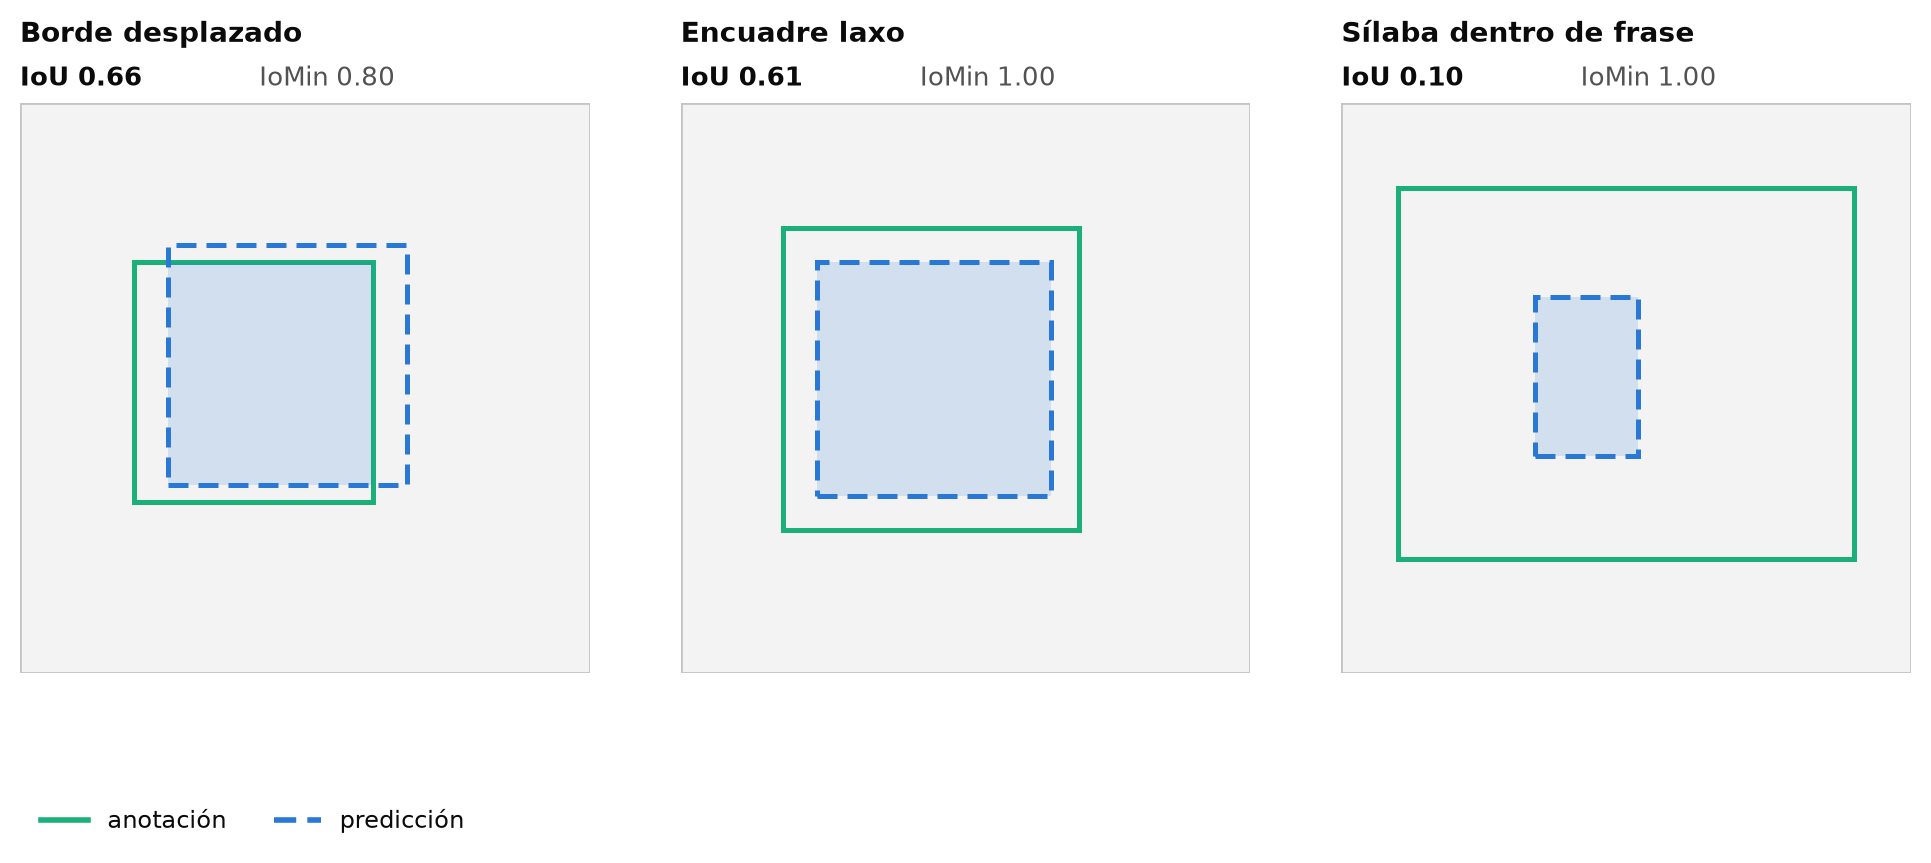
\includegraphics[width=\textwidth]{figures/iou_criterion.png}
    \caption{Criterio de IoU.}
    \label{fig:iou-criterion}
\end{figure}

\paragraph{Fase 6: Despliegue.}
En un proyecto de investigación el despliegue consiste en aplicar el modelo
final a un volumen de grabaciones que no participaron del entrenamiento ni de la
evaluación, y en producir con ellas tablas de anotación automáticas que el
analista pueda abrir directamente en Raven. El artefacto es un \textit{pipeline}
de inferencia que recibe un directorio de audio, aplica exactamente el mismo
preprocesamiento del entrenamiento, obtiene las predicciones crudas, ejecuta el
posprocesamiento y escribe la tabla de selección en el formato esperado.

\subsection{Herramientas}

Cada herramienta se justifica por el requisito que satisface y por la
alternativa que se descarta, no por sus virtudes generales. La
Tabla~\ref{tab:herramientas} recoge las que intervienen en el recorrido del dato
y la Tabla~\ref{tab:herramientas-dev} las que sostienen el desarrollo. Donde no
hay alternativa real, se dice.

\begin{table}[htbp]
    \centering
    \caption[Stack técnico: pipeline]{Herramientas del \textit{pipeline}, de la
        curación a la inferencia}
    \label{tab:herramientas}
    \small
    \begin{tabular}{@{}L{2.5cm}L{4.9cm}L{6.6cm}@{}}
        \toprule
        \textbf{Herramienta}                                                & \textbf{Función en el \textit{pipeline}} & \textbf{Por qué esta y no la alternativa} \\
        \midrule
        Python 3.12                                                         &
        Lenguaje de todo el sistema                                         &
        R y MATLAB carecen de implementaciones de referencia de detectores de
        objetos, que es el componente que no se va a reimplementar                                                                                                 \\
        \addlinespace
        Pandas                                                              &
        Consolidación, limpieza y particionado de las anotaciones tabulares &
        Procesar los archivos de Raven con scripts \textit{ad hoc} no deja
        registro reproducible de qué filas se descartaron y por qué                                                                                                \\
        \addlinespace
        NumPy                                                               &
        Representación en memoria del audio y de las cajas antes de pasar a
        tensores                                                            &
        Sin alternativa práctica: es la interfaz común entre SoundFile, PyTorch
        y Matplotlib                                                                                                                                               \\
        \addlinespace
        SoundFile y soxr                                                    &
        Lectura por bloques de las grabaciones y remuestreo a 44,1\,kHz     &
        Permiten leer solo la ventana pedida de un archivo de una hora, en lugar
        de cargarlo entero en memoria                                                                                                                              \\
        \addlinespace
        torchaudio                                                          &
        Cálculo del espectrograma mel que consume el modelo                 &
        Librosa devuelve arreglos de NumPy y obligaría a convertir en cada lote;
        aquí la transformada entrega tensores que el PCEN entrenable recibe
        directamente                                                                                                                                               \\
        \addlinespace
        PyTorch                                                             &
        Definición, entrenamiento y evaluación del detector                 &
        Las implementaciones de referencia de detectores están mayoritariamente
        en PyTorch, y portarlas a otro marco no se justifica                                                                                                       \\
        \addlinespace
        Transformers                                                        &
        Carga del \textit{backbone} AST preentrenado en AudioSet            &
        Entrenar un transformador de espectrogramas desde cero excede los datos
        disponibles; la biblioteca aporta los pesos y la interpolación del
        \textit{embedding} posicional                                                                                                                              \\
        \addlinespace
        Raven Pro / Lite                                                    &
        Origen de las anotaciones y destino de las predicciones exportadas  &
        Sin alternativa: es la herramienta del analista, y su formato de tabla de
        selección es un requisito de RE2.4, no una elección de diseño                                                                                              \\
        \bottomrule
    \end{tabular}
\end{table}

\begin{table}[htbp]
    \centering
    \caption[Stack técnico: desarrollo]{Herramientas de desarrollo,
        inspección y reproducibilidad}
    \label{tab:herramientas-dev}
    \small
    \begin{tabular}{@{}L{2.5cm}L{4.9cm}L{6.6cm}@{}}
        \toprule
        \textbf{Herramienta}                                             & \textbf{Función} & \textbf{Por qué esta y no la alternativa} \\
        \midrule
        uv                                                               &
        Entorno virtual, resolución de dependencias y archivo de bloqueo &
        Instalar con \textit{pip} sin bloqueo deja libres las versiones
        transitivas, y sin ellas el entorno de una corrida antigua no se
        reconstruye igual                                                                                                               \\
        \addlinespace
        Matplotlib                                                       &
        Figuras del análisis exploratorio y de los resultados            &
        Sin alternativa que aporte algo distinto dentro del mismo ecosistema                                                            \\
        \addlinespace
        PyQt6 y pyqtgraph                                                &
        Visor interactivo que superpone espectrograma, anotación y predicción
        sobre la misma grabación                                         &
        Raven no muestra la salida del modelo junto a la anotación, y una figura
        de Matplotlib no sostiene el desplazamiento continuo sobre una hora de
        audio                                                                                                                           \\
        \addlinespace
        Ruff, ty y pytest                                                &
        Formato, análisis estático y pruebas del código                  &
        Las pruebas cubren la conversión entre sistemas de coordenadas de caja,
        donde un error silencioso desplazaría todas las métricas sin fallar                                                             \\
        \addlinespace
        Git                                                              &
        Versionado del código y de la configuración de cada experimento  &
        Sin alternativa: es la condición para asociar un resultado reportado a
        un estado exacto del código                                                                                                     \\
        \bottomrule
    \end{tabular}
\end{table}

\subsection{Procedimientos y reproducibilidad}

Las fases anteriores describen qué se hace con los datos y por qué. Esta
subsección recoge únicamente lo operativo que no pertenece a ninguna fase en
particular porque atraviesa todas: cómo se custodia el material, cómo se
registran los experimentos y qué garantiza que un número reportado pueda volver a
obtenerse.

\rotulo{Custodia del material primario.} Los audios y sus anotaciones se
mantienen bajo una estructura de directorios fija que no se edita nunca a mano.
Toda transformación se produce por script a partir de ella y escribe en un
directorio derivado distinto. Esa separación es la que permite reconstruir el
conjunto de trabajo desde cero cada vez que el protocolo de curación cambia, y la
que impide que una corrección puntual quede sin registro.

\rotulo{Registro de experimentos.} Cada corrida queda asociada a un identificador
de configuración y a un \textit{commit} del repositorio. El bucle de
entrenamiento registra los hiperparámetros, guarda \textit{checkpoints} de forma
periódica y evalúa sobre validación a intervalos fijos. Los scripts de evaluación
son independientes de los de entrenamiento: cargan un \textit{checkpoint}
existente y recalculan las métricas, de modo que reproducir una cifra publicada
no exige reentrenar.

\rotulo{Respaldo y portabilidad.} El código y la configuración se sincronizan en
un repositorio remoto, y el entorno de ejecución se declara en un archivo de
dependencias versionado, para que la falla del equipo de desarrollo o la
ejecución en una máquina distinta no supongan rehacer trabajo. La gestión de la
bibliografía se centraliza en Zotero a lo largo de todo el proceso.

La planificación que ordena todo lo anterior en el tiempo, mediante la estructura de
desglose del trabajo, el cronograma, el presupuesto y la gestión de riesgos, se recoge
en el Anexo~\ref{anx:plan}, fuera del cuerpo, porque no aporta al argumento
científico y en el hilo del documento lo interrumpiría.


% ===================================================================
% CAPÍTULO 2
% ===================================================================
\chapter{Marco Referencial}
\label{cap:marco}

\section{Marco Teórico}

\subsection{Formulación del problema de detección}
\label{sec:formulacion}

El problema se plantea en dos niveles. El nivel de la \emph{grabación} es el que
le interesa al analista y define el producto; el nivel de la \emph{ventana} es el
que consume el modelo y define su entrada y su salida. Separarlos es necesario
porque ninguna arquitectura actual procesa una hora de audio de una sola vez, y
confundirlos oscurece qué predice realmente un detector.

\paragraph{Nivel de grabación}
El sistema recibe un conjunto de grabaciones $G=\{g_1,g_2,\dots,g_M\}$. Cada
grabación $g_k$ es una señal de audio $x(t)$ en formato WAV, muestreada a
$F_s = 44{,}1$\,kHz, de duración $D_k$ que puede llegar a la hora. Para cada una
el sistema debe devolver una lista de eventos $E_k=\{e_1,e_2,\dots,e_{N_k}\}$,
cuyo cardinal $N_k$ no se conoce de antemano y donde cada evento es la tupla

\begin{equation}
    e_i = \bigl(t^{(i)}_{\text{ini}},\; t^{(i)}_{\text{fin}},\;
    f^{(i)}_{\min},\; f^{(i)}_{\max},\;
    y^{(i)},\; p^{(i)}\bigr).
    \label{eq:tupla}
\end{equation}

\begin{description}
    \item[$(t_{\text{ini}}, t_{\text{fin}})$] Instantes de inicio y fin del
          evento, en segundos desde el comienzo de la grabación, con
          $0 \le t_{\text{ini}} < t_{\text{fin}} \le D_k$.

    \item[$(f_{\min}, f_{\max})$] Banda de frecuencia que ocupa el evento, en
          hercios, con $0 \le f_{\min} < f_{\max} \le F_s/2$. Es la componente que
          distingue esta formulación de la detección de eventos sonoros puramente
          temporal.

    \item[$y$] Etiqueta tomada de un vocabulario cerrado
          $Y=\{y_1,\dots,y_L\}$ cuyos elementos son pares de especie y tipo de
          llamada. La sección~\ref{sec:etiqueta} justifica por qué la etiqueta es un
          par plano y no dos niveles predichos por separado; las proyecciones
          $\pi_{\text{esp}}(y)$ y $\pi_{\text{tipo}}(y)$ recuperan cada nivel cuando
          se lo necesita.

    \item[$p$] Confianza en $[0,1]$ asignada por el modelo, que ordena las
          predicciones y define el punto de operación de la revisión asistida.
\end{description}

Las cuatro primeras componentes definen una caja rectangular sobre el plano
tiempo--frecuencia; las dos restantes la etiquetan y la puntúan. La
Figura~\ref{fig:segmentacion} muestra el resultado sobre un espectrograma.

\begin{figure}[htbp]
    \centering
    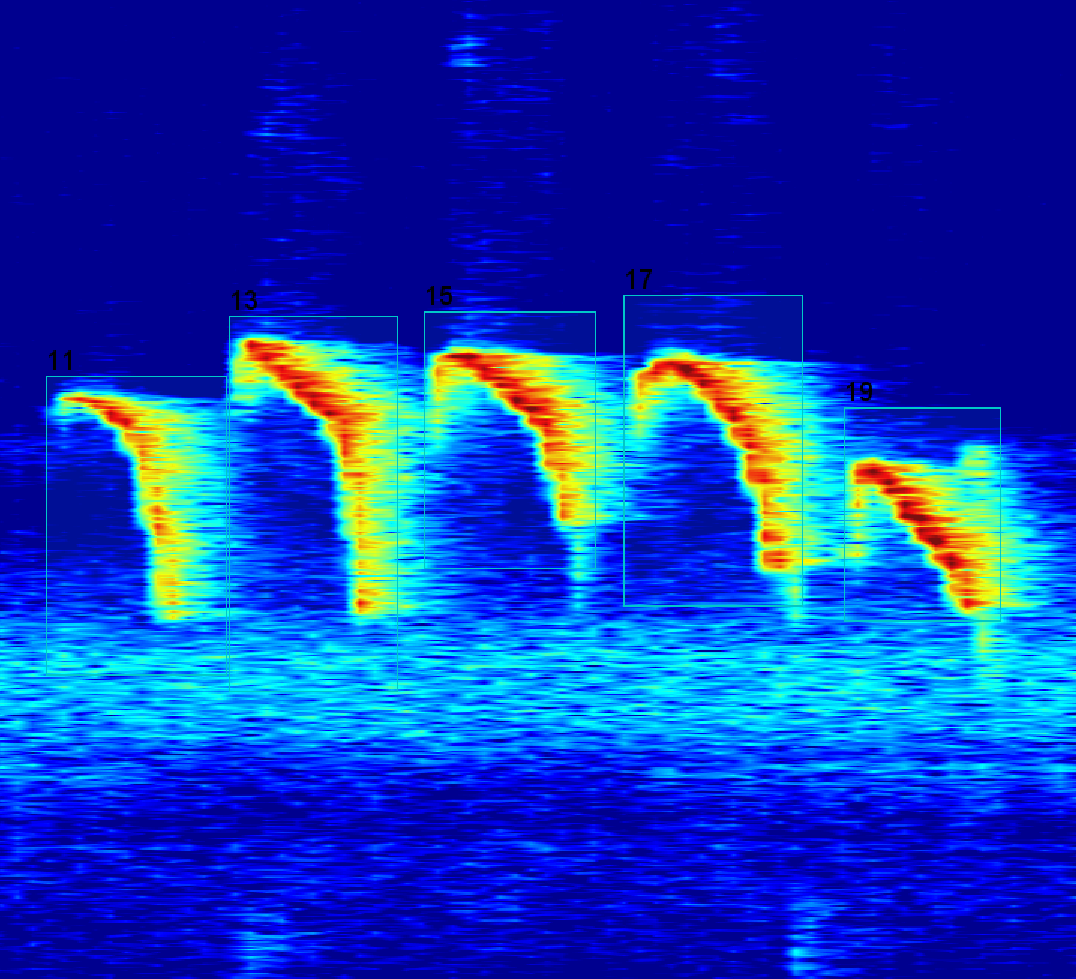
\includegraphics[width=0.72\textwidth]{figures/image3.png}
    \caption[Segmentación tiempo--frecuencia]{Segmentación de audio en rangos de
        tiempo y frecuencia sobre un espectrograma. Cada rectángulo corresponde a una
        tupla de la ecuación~\eqref{eq:tupla}.}
    \label{fig:segmentacion}
\end{figure}

\paragraph{Nivel de ventana}
La grabación se recorta en ventanas de duración fija $T_w$, tomadas cada $H$
segundos con $H < T_w$, de modo que ningún evento quede siempre partido por un
borde. Cada ventana se convierte en un espectrograma mel
$X \in \mathbb{R}^{F \times T}$, con $F$ bandas de frecuencia y $T$ tramas
temporales, y ese tensor es la entrada del modelo.

El detector es una función de parámetros $\theta$ que a cada ventana le asigna un
conjunto de tamaño fijo

\begin{equation}
    f_\theta(X) = \bigl\{(\hat{b}_q,\; \hat{\pi}_q)\bigr\}_{q=1}^{Q},
    \qquad
    \hat{b}_q \in [0,1]^4,
    \qquad
    \hat{\pi}_q \in [0,1]^{L+1},
    \label{eq:modelo}
\end{equation}

donde $Q$ es un número de consultas fijado por la arquitectura, independiente del
contenido de la ventana y mayor que la cantidad de eventos que cabe esperar en
ella. Cada consulta produce una caja $\hat{b}_q = (c_x, c_y, w, h)$ en
coordenadas normalizadas al recuadro de la ventana --- centro, ancho y alto, los
cuatro en $[0,1]$ --- y una distribución $\hat{\pi}_q$ sobre
$Y \cup \{\varnothing\}$, en la que $\varnothing$ es la clase «sin objeto» que
absorbe las consultas sobrantes. El número de eventos no se predice: resulta de
cuántas consultas eligen una clase de $Y$ por encima del umbral de confianza.

Esta es la formulación de \emph{predicción de conjuntos}: la salida no es una
rejilla puntuada ni una secuencia, sino un conjunto sin orden, y durante el
entrenamiento cada anotación de la ventana se asigna a exactamente una consulta
mediante un emparejamiento biyectivo, mientras que el resto se supervisa hacia
$\varnothing$. De ahí que dentro de la ventana no haya anclas ni supresión de no
máximos.

\paragraph{Del marco normalizado al marco físico}
Lo que emite el modelo no son segundos ni hercios sino fracciones de la ventana,
y la conversión no es simétrica entre los dos ejes. En tiempo es afín: si la
ventana empieza en $t_0$,
\begin{equation}
    t_{\text{ini}} = t_0 + \bigl(c_x - \tfrac{w}{2}\bigr) T_w,
    \qquad
    t_{\text{fin}} = t_0 + \bigl(c_x + \tfrac{w}{2}\bigr) T_w.
\end{equation}
En frecuencia no lo es, porque el eje vertical del espectrograma está en escala
mel. Con $m(\cdot)$ la función que convierte hercios a mel y $[f_{\text{lo}},
            f_{\text{hi}}]$ los extremos del banco de filtros, la coordenada normalizada
$u \in [0,1]$ vuelve a hercios mediante
\begin{equation}
    \varphi(u) = m^{-1}\!\bigl(m(f_{\text{lo}}) + u\,[\,m(f_{\text{hi}}) -
            m(f_{\text{lo}})\,]\bigr),
    \label{eq:mel-inv}
\end{equation}
y entonces $f_{\min} = \varphi(c_y - h/2)$ y $f_{\max} = \varphi(c_y + h/2)$. La
consecuencia práctica es que una caja de altura constante en el marco normalizado
cubre una banda mucho más ancha en la parte alta del espectro que en la baja.

\paragraph{De las ventanas a la grabación}
Como las ventanas se solapan, una misma vocalización puede predecirse en dos o
tres de ellas, y una vocalización más larga que $T_w$ solo puede predecirse por
partes. Las predicciones de toda la grabación se llevan al marco común, se
agrupan por clase y se depuran por supresión de no máximos, de modo que la lista
$E_k$ contenga un evento por vocalización. Ese es el punto en el que el nivel de
ventana devuelve el control al nivel de grabación, y también el punto en el que
el ventaneo deja su huella: la sección~\ref{sec:ventaneo} documenta qué eventos
quedan fuera de alcance por ser más largos que la ventana.

\subsection{El espectrograma y la asimetría de sus ejes}

La señal de audio es unidimensional, pero los eventos de interés se distinguen
por cómo se distribuye su energía entre frecuencias a lo largo del tiempo. La
transformada de Fourier de tiempo corto (STFT) recupera esa estructura: divide
la señal en tramas solapadas, aplica una ventana a cada una y calcula su
espectro. La magnitud del resultado es el espectrograma, una matriz
$X \in \mathbb{R}^{F\times T}$ cuyos parámetros, como el tamaño de ventana, el salto
entre ventanas y el tipo de ventana, fijan el compromiso entre resolución
temporal y resolución frecuencial.

Las transformaciones que se aplican sobre esa matriz, como la escala mel, la compresión
logarítmica y la normalización de energía por canal, y el criterio con el que se
elige entre ellas se tratan en la sección~\ref{sec:representacion}, donde
corresponden al eslabón de la cadena en que aparece esa decisión.

Interesa aquí una asimetría del espectrograma que conviene explicitar porque condiciona el
diseño del detector. Tratarlo como una imagen es útil, pero sus dos ejes no son
equivalentes: una traslación en tiempo preserva el significado del patrón,
mientras que una traslación en frecuencia lo cambia: un mismo contorno
desplazado media octava es otra vocalización, o ninguna. Los patrones
espectro-temporales de los eventos sonoros dependen de la banda de frecuencia en
que ocurren, de modo que la convolución bidimensional estándar, equivariante a
traslación en ambos ejes, no es adecuada para el eje frecuencial
\citep{nam_frequency_2022}. La consecuencia práctica es que el modelo debe
conservar de forma explícita la posición en frecuencia en lugar de descartarla.

\subsection{Detección de objetos sobre audio}
\label{sec:objetos}

Una vez que el sonido se representa como una matriz tiempo--frecuencia, la tarea
de la ecuación~\eqref{eq:tupla} coincide con la de la detección de objetos en
visión por computadora: afirmar que una clase está presente y localizarla,
localización que se representa típicamente mediante una caja delimitadora
\citep{lin_2014}. La analogía no es superficial. Los eventos acústicos se
manifiestan como patrones bidimensionales de tiempo y frecuencia, con texturas y
estructuras geométricas propias, análogos a los objetos que aparecen en imágenes
naturales \citep{pham_eventness_2018}, y el encuadre trasciende la bioacústica
hacia el análisis de señales en general \citep{wood_deep_2022}.

\rotulo{Familia R-CNN.} Los detectores de dos etapas proponen primero regiones
candidatas y luego las clasifican y refinan. Su aplicación a espectrogramas está
documentada en bioacústica marina, donde las cajas predichas llevan información
estadística embebida sobre la vocalización, como su duración, ancho de banda y
frecuencia central, directamente utilizable por el analista
\citep{escobar-amado_computer_2024}. NBM adapta un detector de dos etapas a
datos de audio y lo acompaña de anotaciones precisas en tiempo y frecuencia
recolectadas por aficionados \citep{airale_nbm_2025}.

\rotulo{Familia YOLO.} Los detectores de una etapa predicen clase y caja en una
sola pasada sobre una rejilla, lo que los hace más rápidos y más simples de
entrenar. Su uso sobre espectrogramas está reportado como línea base competitiva
\citep{gonzalez_yolo-based_2025}. En audio, la idea de regresar directamente los
límites del evento en lugar de clasificar tramas aparece también en YOHO, que
convierte la detección en una regresión de los puntos de inicio y fin de cada
clase \citep{venkatesh_you_2022}.

\rotulo{Familia DETR y transformadores.} Los detectores basados en atención
eliminan las anclas y la supresión de no máximos, y formulan la detección como
la predicción directa de un conjunto de objetos emparejado con las anotaciones.
Su adaptación al audio es reciente: SoundDet trata el audio crudo como una señal
espacio-temporal y detecta eventos móviles sobre ella \citep{he_sounddet_2021},
y \citet{ebbers_sound_2024} formalizan la salida como cuádruplas de clase,
inicio, fin y confianza, aunque manteniéndola sobre el eje temporal.

\rotulo{Cajas frente a máscaras.} Una alternativa a la caja es la segmentación
semántica, que asigna una etiqueta a cada celda tiempo--frecuencia y describe
con más fidelidad los contornos de una vocalización \citep{jin_semantic_2022}.
Esta tesis opta por la caja por dos razones: es la forma en que el analista
anota en Raven, y por tanto la única para la que existe una referencia
disponible; y es la que se exporta sin pérdida a una tabla de selección. Una
máscara exigiría reanotar el corpus completo.

\section{Marco Conceptual}

Los conceptos que siguen no se presentan por área temática sino siguiendo el
recorrido de la señal, desde que el animal vocaliza hasta que el analista recibe
una etiqueta revisable. Cada eslabón de ese recorrido pierde algo o introduce una
ambigüedad, y es esa pérdida la que crea la necesidad del eslabón siguiente. El
orden de las subsecciones es, por tanto, el orden en que aparecen los problemas.

\begin{figure}[htbp]
    \centering
    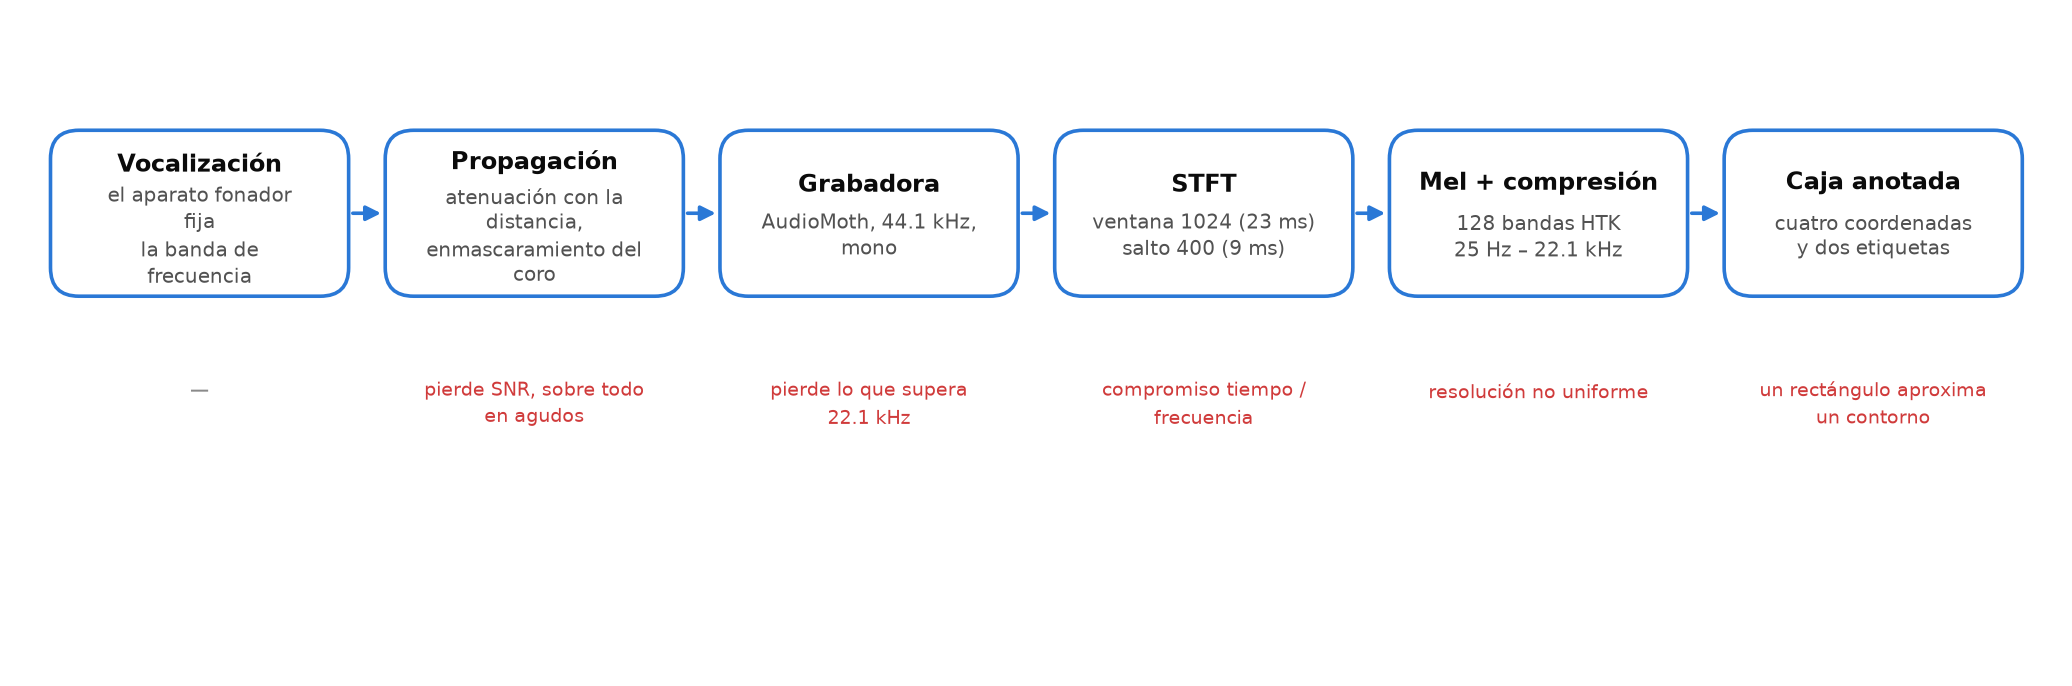
\includegraphics[width=\textwidth]{figures/signal_chain.png}
    \caption{Cadena de la señal.}
    \label{fig:signal-chain}
\end{figure}

\subsection{Paisaje sonoro}

La bioacústica estudia el sonido en los seres vivos. En este proyecto se aplica
a través del monitoreo acústico pasivo, que despliega grabadoras autónomas para
capturar el paisaje sonoro de un ecosistema sin intervenir en él
\citep{blumstein_acoustic_2011}. Lo que la grabadora registra no es la
vocalización sino la suma de todo lo que llega al micrófono, y en un entorno como
la Amazonía esa suma tiene tres componentes:

\begin{description}
    \item[Biofonía.] Los sonidos de origen biológico. Incluye la señal de interés
          las vocalizaciones de primates y también el coro de insectos, anfibios
          y aves, que ocupa las mismas bandas durante horas seguidas.

    \item[Geofonía.] Los sonidos de origen físico: viento, lluvia, movimiento de
          la vegetación. Su energía se reparte sobre bandas amplias y su carácter es
          o bien cuasi-estacionario o bien de ráfaga.

    \item[Antropofonía.] Los sonidos de origen humano: motosierras, disparos,
          motores. No solo interfieren con la señal, sino que son en sí mismos un
          indicador de presión sobre el ecosistema \citep{blumstein_acoustic_2011}.
\end{description}

A ello se suma la atenuación: el animal está a una distancia desconocida del
sensor, de modo que la misma vocalización llega unas veces nítida y otras apenas
por encima del fondo. El archivo resultante contiene, entonces, una señal
mezclada, atenuada y de relación señal-ruido variable dentro de una misma
grabación. La pregunta que abre el eslabón siguiente es qué hay que buscar dentro
de esa mezcla, es decir, qué constituye exactamente un evento.

\subsection{Eventos acústicos}

La vocalización se produce por el flujo de aire desde los pulmones, que hace
vibrar las cuerdas vocales en la laringe y actúa como fuente sonora primaria; el
tracto vocal supralaríngeo, formado por la faringe y las cavidades oral y nasal,
filtra esa fuente
y fija sus características finales: frecuencia fundamental, distribución de
armónicos, amplitud, duración y timbre.

La consecuencia de esa estructura fuente--filtro es la que interesa aquí. La
frecuencia fundamental queda determinada por la geometría y la tensión de las
cuerdas vocales, y las resonancias del tracto vocal concentran la energía en un
conjunto acotado de bandas. Un evento no es, por tanto, un instante con una
etiqueta: es una región del plano tiempo--frecuencia con un límite inferior y un
límite superior de frecuencia que dependen de la anatomía de quien vocaliza. La
banda que ocupa una especie es una propiedad física de su aparato fonador, no una
convención de dibujo del anotador. Esa es la razón por la que la caja
tiempo--frecuencia de la ecuación~\eqref{eq:tupla} es la representación adecuada
del evento, y no un rectángulo elegido por comodidad: los cuatro números que la
definen tienen referente físico.

La misma estructura explica dos hechos que reaparecen más adelante. El primero es
que distintas especies tienden a separarse por banda, lo que hace de la
frecuencia una característica discriminante y no un dato accesorio. El segundo es
que la producción vocal en primates no humanos es en gran medida innata y ligada
a estados internos, con control cortical limitado, pero admite variabilidad
intraespecífica, incluidos dialectos, firmas individuales y variación según el
contexto, que amplía el rango de formas que el detector debe reconocer como la
misma clase.

El evento existe, entonces, como región bidimensional. El problema es que la
señal grabada es unidimensional: hay que recuperar esa estructura antes de poder
buscarla.

\subsection{Representaciones tiempo--frecuencia}
\label{sec:representacion}

La transformada de Fourier de tiempo corto recupera la dimensión que falta:
divide la señal en tramas solapadas y calcula el espectro de cada una, con lo que
produce una matriz $X \in \mathbb{R}^{F \times T}$ en la que el eje vertical es
frecuencia y el horizontal, tiempo. Sobre ella se aplican dos transformaciones
habituales: la escala mel, que reagrupa las bandas según una progresión
aproximadamente logarítmica, y la compresión logarítmica de la magnitud a
decibelios. El resultado, el espectrograma log-mel, es la entrada estándar en
detección de eventos sonoros.

Esta transformación es la bisagra del planteamiento: convierte un problema de
audio en un problema de análisis de imágenes, y con ello habilita el uso de las
técnicas de visión por computadora descritas en la sección~\ref{sec:formulacion}
y siguientes.

La elección de la representación no es un trámite. La compresión logarítmica no
es la única opción. La normalización de energía por
canal (PCEN) combina control adaptativo de ganancia y compresión de rango
dinámico, y en detección bioacústica de campo fue el contribuyente principal a la
mejora de precisión sobre la línea base log-mel \citep{lostanlen_robust_2019}. El
criterio que decide entre ambas no es esa cifra sino una condición del ruido: la
ventaja de PCEN proviene de estimar y descontar un fondo que varía lentamente
respecto de la escala temporal del evento. El coro de insectos amazónico cumple
esa condición, pues es cuasi-estacionario durante minutos, pero la lluvia y las
ráfagas de viento no la cumplen, y sobre ellas el control de ganancia puede
atenuar la propia vocalización junto con el fondo.

Dado que el corpus contiene ambos regímenes, esta tesis no da por establecida la
superioridad de ninguna de las dos representaciones: las compara bajo un criterio
declarado de antemano: el \textit{recall} de eventos de baja relación
señal-ruido al punto de operación fijado en la sección~\ref{sec:metodos}, y
adopta la que lo maximice. Declarar el criterio antes de medir es lo que impide
elegir después la representación que favorezca al resultado obtenido.

Queda así una imagen en la que el evento es visible. Falta el mecanismo que lo
localice dentro de ella.

\begin{figure}[htbp]
    \centering
    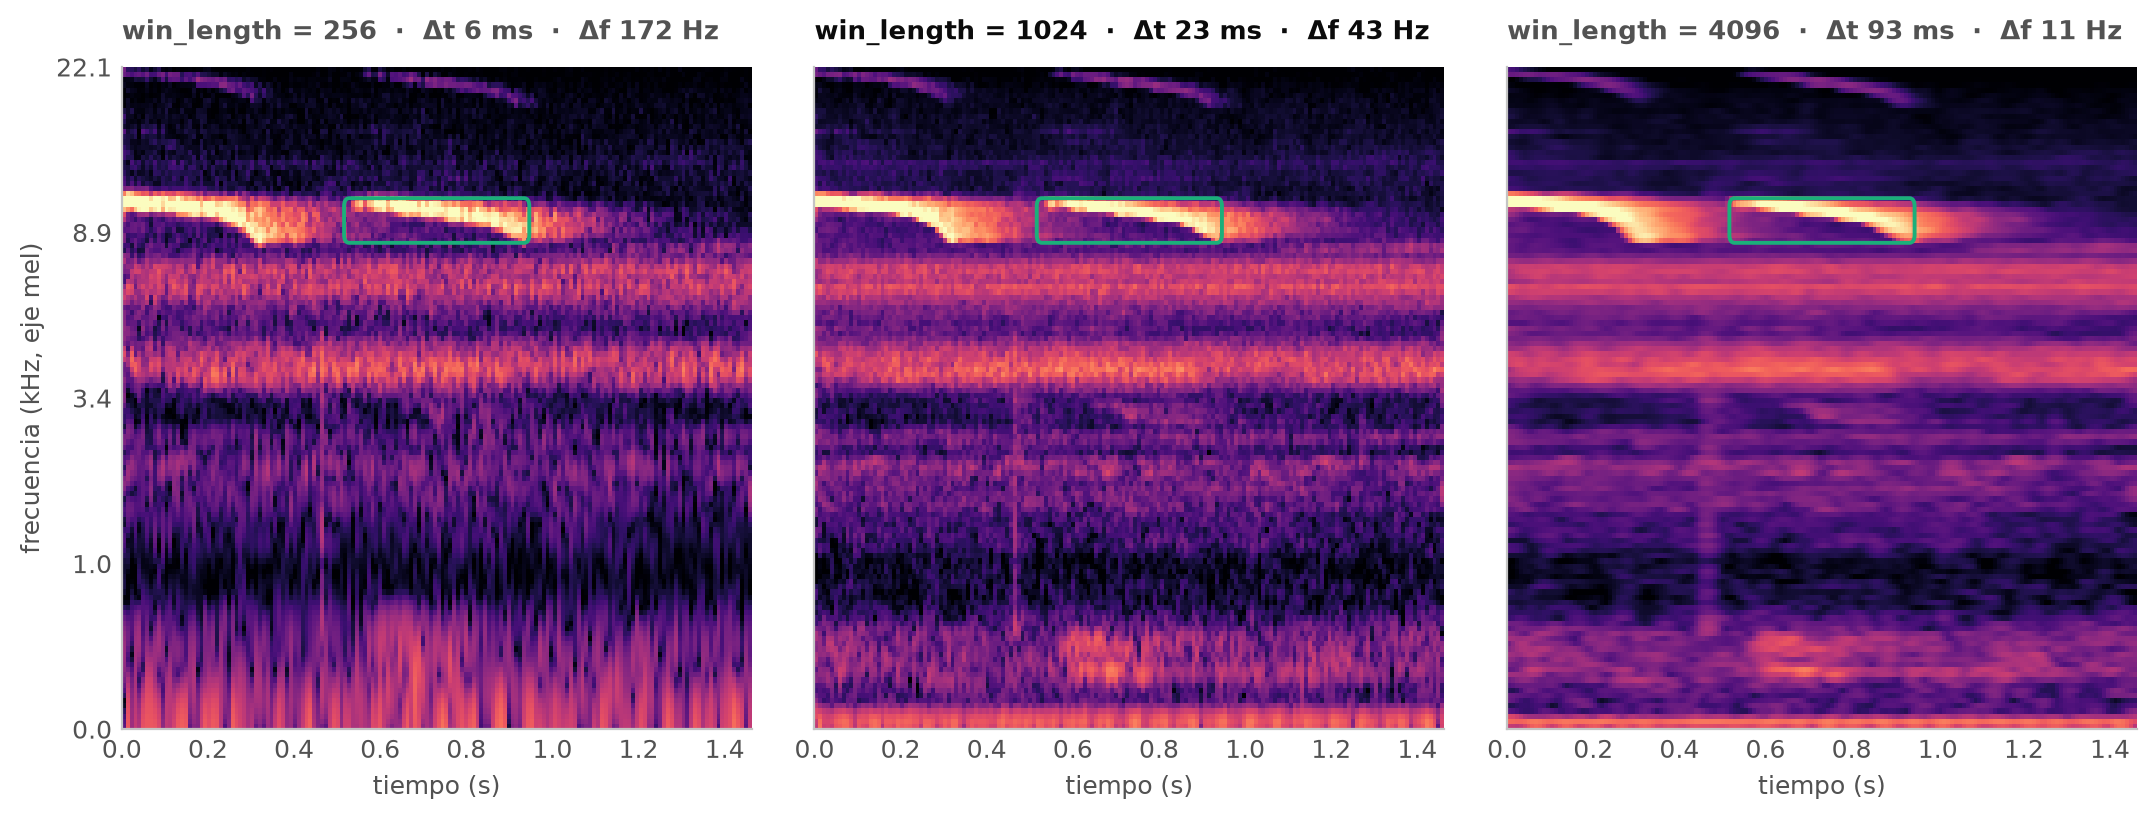
\includegraphics[width=\textwidth]{figures/stft_tradeoff.png}
    \caption{Compromiso STFT.}
    \label{fig:stft-tradeoff}
\end{figure}

\begin{figure}[htbp]
    \centering
    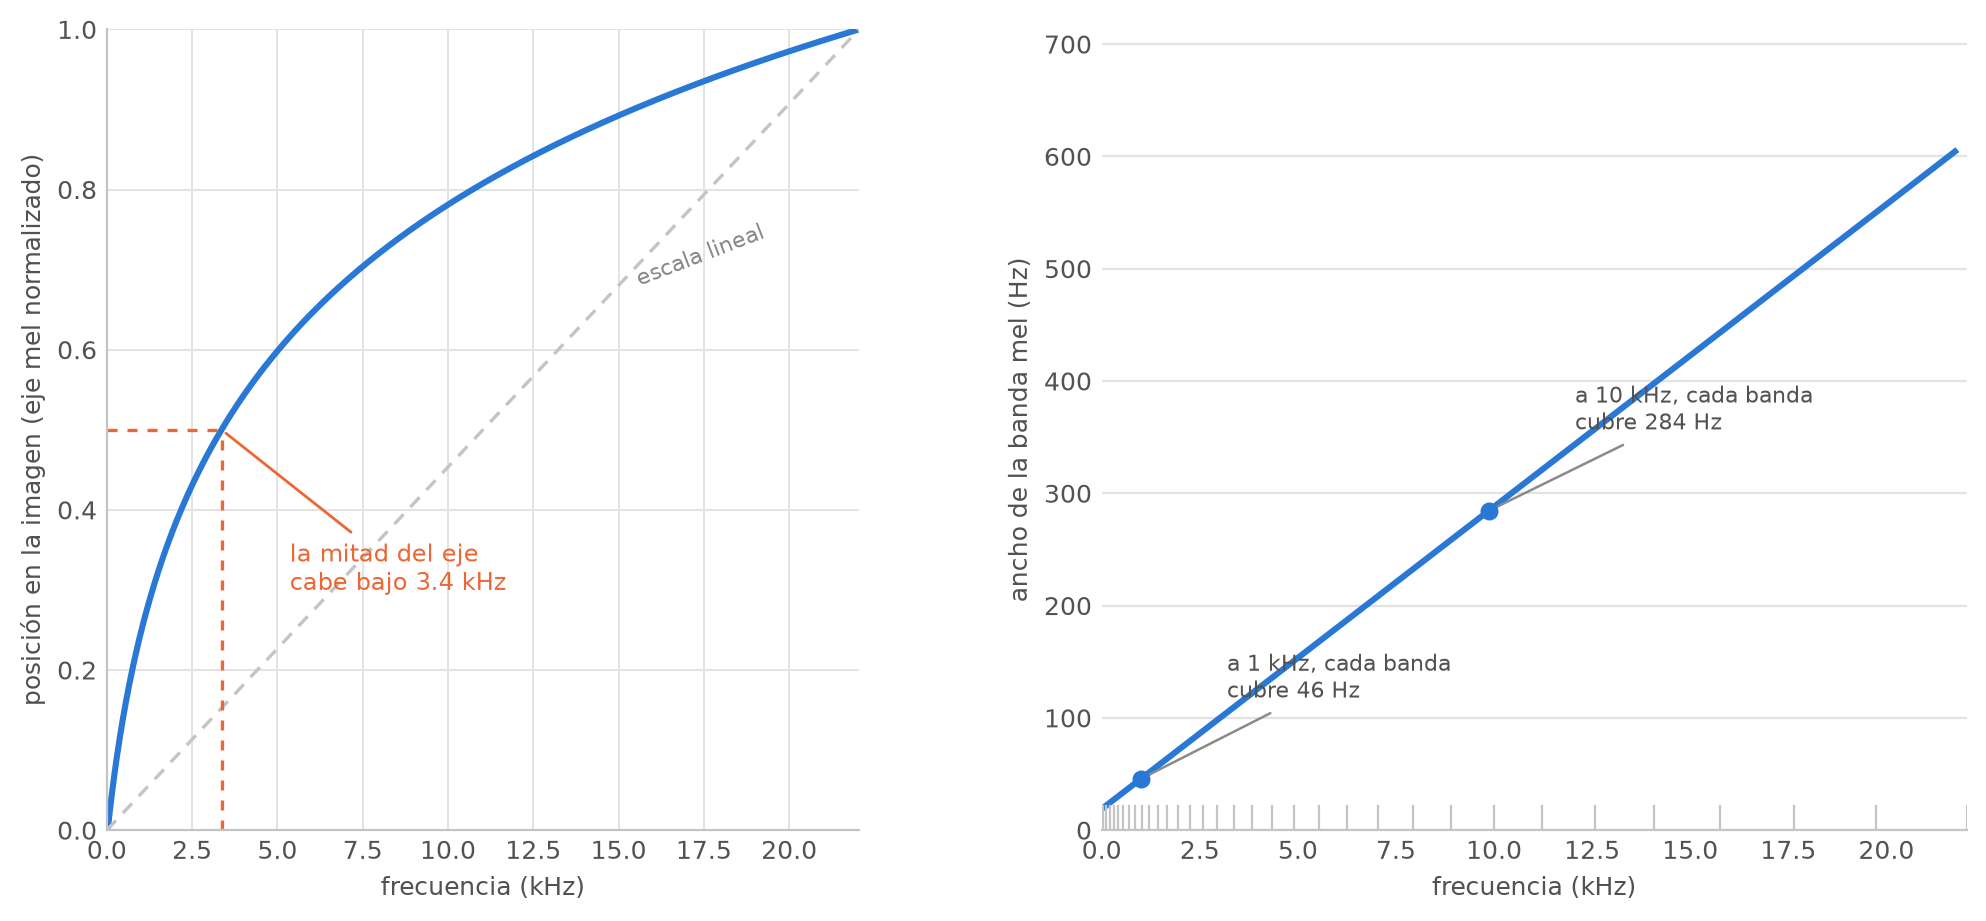
\includegraphics[width=\textwidth]{figures/mel_axis.png}
    \caption{Escala mel.}
    \label{fig:mel-axis}
\end{figure}

\begin{figure}[htbp]
    \centering
    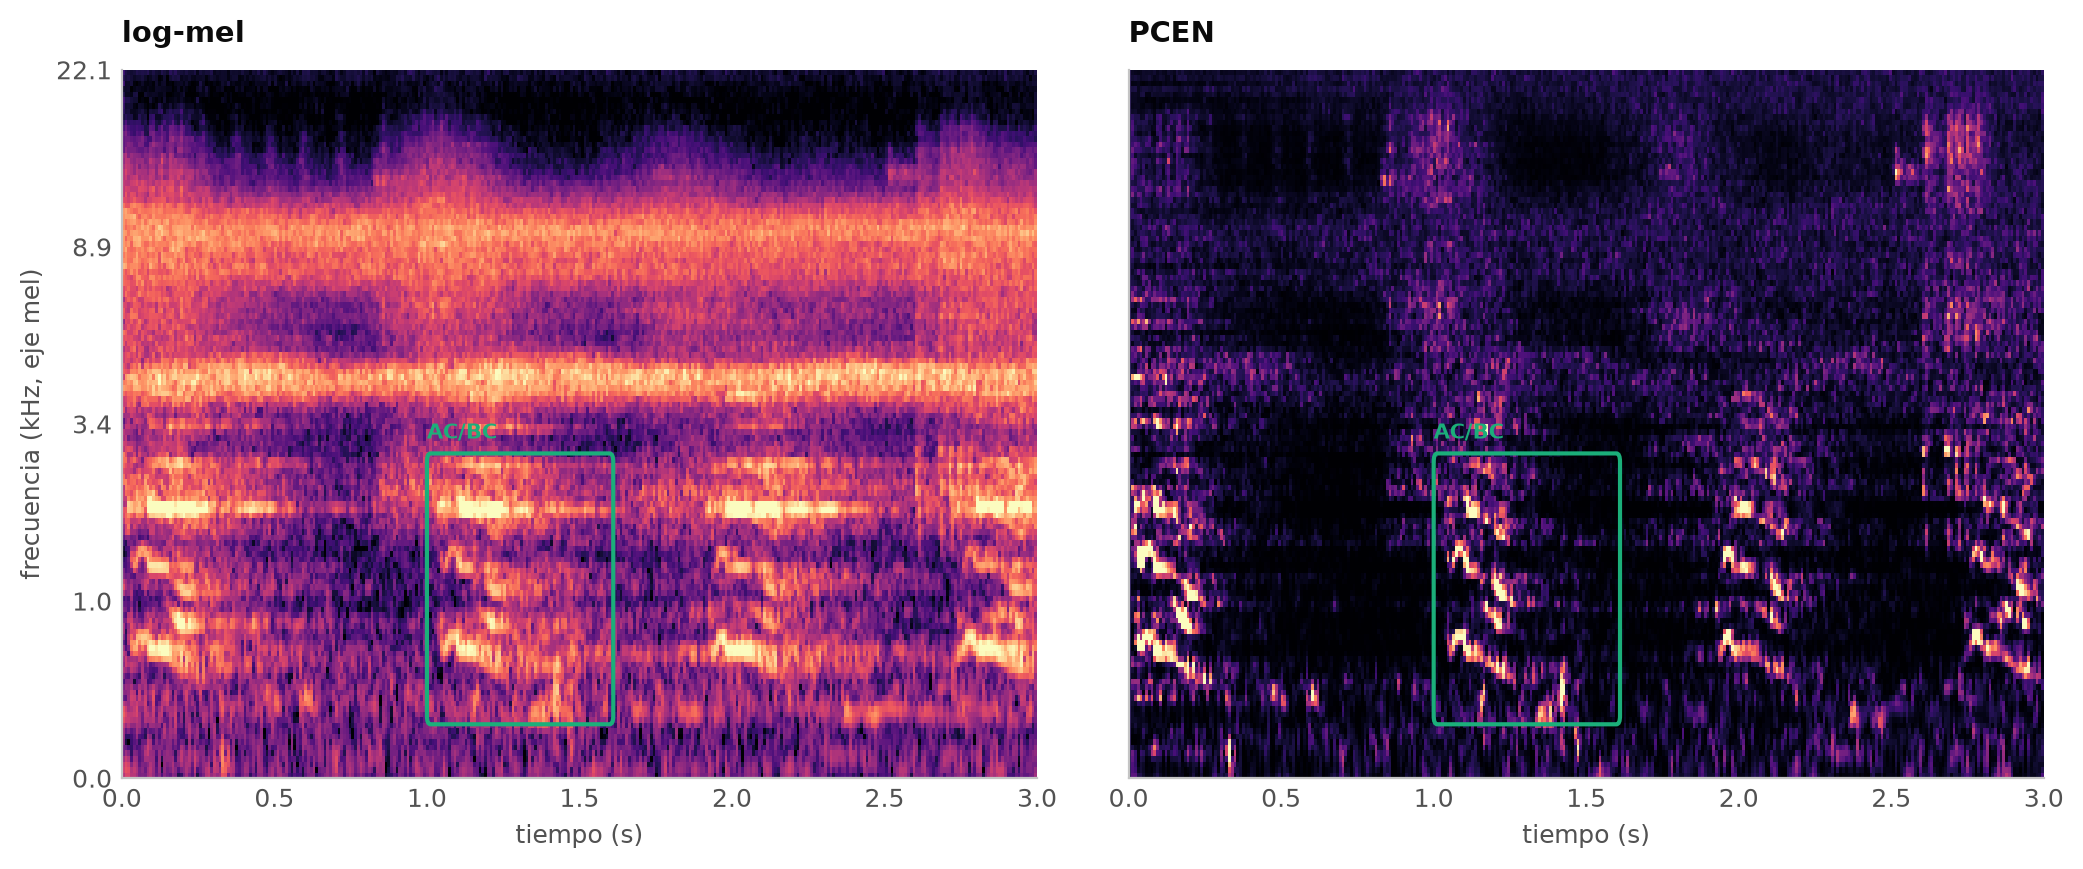
\includegraphics[width=\textwidth]{figures/pcen_vs_logmel.png}
    \caption{PCEN frente a log-mel.}
    \label{fig:pcen-vs-logmel}
\end{figure}

\subsection{Detección de eventos sonoros}

La detección de eventos sonoros (SED) consiste en identificar la presencia de un
evento y localizar sus límites sobre la representación tiempo--frecuencia. La
distinción decisiva dentro de esta tarea, que además constituye el concepto central de esta
tesis, es la \emph{forma de la salida}, porque no todas las formulaciones que
se llaman SED devuelven un evento.

\rotulo{Salida por segmento fijo.} El sistema divide la grabación en fragmentos
de duración constante y emite una probabilidad por fragmento y clase. Lo que
devuelve es una rejilla puntuada, no un evento: el inicio y el fin de la
vocalización quedan cuantizados al tamaño del fragmento, y su banda de frecuencia
sencillamente no se estima.

\rotulo{Salida temporal delimitada.} El sistema devuelve el instante de inicio y
el de fin de cada evento, con su clase y su confianza. Es ya un evento con
extensión propia, pero esa extensión existe solo sobre el eje temporal: descarta
$f_{\min}$ y $f_{\max}$, que la subsección anterior estableció como magnitudes
físicas del aparato fonador.

\rotulo{Salida tiempo--frecuencia.} El sistema devuelve la tupla completa de la
ecuación~\eqref{eq:tupla}. Es la única de las tres formas que coincide con lo que
el analista produce a mano en Raven y, por tanto, la única que puede sustituir su
insumo en lugar de complementarlo.

Esta gradación es exactamente la causa C3 del árbol de problemas del
Capítulo~\ref{cap:generalidades}: la salida de los sistemas automáticos no
sustituye el trabajo del analista porque su representación es más pobre que la
del evento anotado. El marco conceptual la enuncia aquí como propiedad de la
tarea; la sección~\ref{sec:vacio} la usó como argumento de posicionamiento.

El problema impone seis exigencias, y cada familia de la literatura responde a
una de ellas. Presentarlas en orden cronológico no dice nada; presentarlas por la
exigencia que satisfacen permite decidir, y así las ordena la
Tabla~\ref{tab:familias}. Las vocalizaciones de primates se organizan en
secuencias cuya identidad depende del orden y del espaciado de sus unidades, lo
que explica por qué el contexto largo aparece como exigencia propia y no como un
refinamiento del reconocimiento local.

\begin{table}[htbp]
    \centering
    \caption[Arquitecturas frente a requisitos]{Cada exigencia del problema y la
        familia de arquitecturas que la resuelve}
    \label{tab:familias}
    \small
    \begin{tabular}{@{}L{4.0cm}L{3.4cm}L{7.2cm}@{}}
        \toprule
        \textbf{Exigencia}                                     & \textbf{Familia} & \textbf{Qué aporta y dónde se queda corta} \\
        \midrule
        Reconocer un patrón espectro-temporal local            &
        Redes convolucionales                                  &
        Aplican filtros sobre vecindades del espectrograma y superan con claridad
        a los detectores por energía o por flujo espectral, pero una red simple
        carece de robustez frente a la variabilidad del ruido
        \citep{lostanlen_robust_2019}                                                                                          \\
        \addlinespace
        Sostener el contexto a lo largo de una frase           &
        Convolucionales recurrentes                            &
        Añaden capas recurrentes sobre las características convolucionales; fueron
        la arquitectura predominante en las primeras ediciones de los desafíos de
        localización y detección de eventos sonoros \citep{politis_dataset_2020}                                               \\
        \addlinespace
        Ganar profundidad sin degradación                      &
        Conexiones residuales                                  &
        Permiten entrenar redes muy profundas sin pérdida de desempeño
        \citep{he_deep_2016}; BirdNET, referencia en identificación de aves,
        emplea una arquitectura de esa familia \citep{kahl_birdnet_2021}                                                       \\
        \addlinespace
        Modelar dependencias a larga distancia sin recurrencia &
        Transformadores                                        &
        Autoatención y procesamiento paralelo; el \textit{Audio Spectrogram
            Transformer} aparece como innovación en detección bioacústica de pocos
        ejemplos \citep{nolasco_learning_2023}, pero produce representaciones de
        una sola escala                                                                                                        \\
        \addlinespace
        Preservar la posición en frecuencia                    &
        Ninguna de las anteriores por sí sola                  &
        La convolución bidimensional estándar es equivariante a traslación en
        ambos ejes, propiedad deseable en tiempo y errónea en frecuencia;
        corregirlo exige adaptar el filtro a la banda \citep{nam_frequency_2022}                                               \\
        \addlinespace
        Emitir $f_{\min}$ y $f_{\max}$                         &
        Cabezas de detección de objetos                        &
        Única salida que coincide con la tupla de la ecuación~\eqref{eq:tupla};
        es la familia descrita en la sección~\ref{sec:objetos}                                                                 \\
        \bottomrule
    \end{tabular}
\end{table}

El criterio de descarte es la forma de la salida, no el desempeño reportado. Una
arquitectura solo es candidata a arquitectura final si su cabeza puede emitir
$f_{\min}$ y $f_{\max}$. Bajo esa regla, las cuatro primeras familias de la
Tabla~\ref{tab:familias} quedan descartadas \emph{como sistema
    completo}, porque su formulación habitual termina en una probabilidad por trama o
por segmento; ninguna queda descartada \emph{como extractor de características},
que es el papel en el que siguen siendo pertinentes. La cabeza que sí satisface
la exigencia es la de los detectores de objetos descritos en la
sección~\ref{sec:objetos}, y por eso la arquitectura de esta tesis combina un
extractor de audio con una cabeza de detección, en lugar de adoptar una de las
cuatro familias tal como se emplean en la literatura de SED.

Localizado el evento, queda el problema de nombrarlo.

\subsection{Clasificación jerárquica}
\label{sec:etiqueta}

La etiqueta que el analista necesita contiene dos niveles anidados,
la especie y, dentro de su repertorio, el tipo de llamada. Las unidades acústicas se agrupan en notas,
trinos, sílabas, frases, motivos y cantos, y pueden estar jerárquicamente anidadas:
una secuencia de unidades puede considerarse ella misma una unidad y ser reemplazada por una
etiqueta única \citep{kershenbaum_acoustic_2016}.

El conjunto de especies sobre el que se define el primer nivel es el de la
Tabla~\ref{tab:especies}. Los códigos de dos letras de la última columna son los
que se emplean en el resto del documento.

\begin{table}[htbp]
    \centering
    \caption{Especies de primates consideradas en el proyecto}
    \label{tab:especies}
    \small
    \begin{tabular}{@{}L{4.3cm}L{4.3cm}L{4.2cm}c@{}}
        \toprule
        \textbf{Nombre común (inglés)} & \textbf{Nombre común (español)}                     & \textbf{Nombre científico}            & \textbf{Código} \\
        \midrule
        Weddell's saddle-back tamarin  & Tamarino de Weddell / pichico de vientre anaranjado & \textit{Leontocebus weddelli}         & LW              \\
        \addlinespace
        Toppin's titi monkey           & Tití de Toppin / huicoco                            & \textit{Plecturocebus toppini}        & PT              \\
        \addlinespace
        Shock-headed capuchin          & Capuchino de cabeza chata / machín blanco           & \textit{Cebus cuscinus}               & CC              \\
        \addlinespace
        Peruvian spider monkey         & Mono araña peruano / maquisapa                      & \textit{Ateles chamek}                & AC              \\
        \addlinespace
        Night monkey                   & Mono nocturno / musmuqui                            & \textit{Aotus azarae}                 & AA              \\
        \addlinespace
        Large-headed capuchin          & Capuchino de cabeza grande / machín negro           & \textit{Sapajus apella macrocephalus} & SM              \\
        \addlinespace
        Bolivian red howler            & Mono aullador rojo boliviano / coto mono            & \textit{Alouatta sara}                & AS              \\
        \addlinespace
        Bolivian squirrel monkey       & Mono ardilla boliviano / fraile                     & \textit{Saimiri boliviensis}          & SB              \\
        \bottomrule
    \end{tabular}
\end{table}

El segundo nivel de la etiqueta se define dentro de cada especie, sobre el
vocabulario de la Tabla~\ref{tab:repertorio}. Los repertorios estan desbalanceados, de modo que los 41
pares posibles no se reparten de forma pareja entre las ocho especies, y esa
asimetría es la que condiciona la elección del esquema de clasificación.

\begin{table}[htbp]
    \centering
    \small
    \begin{threeparttable}
        \caption[Repertorio por especie]{Tipos de llamada admitidos en cada
            especie, con el código que aparece en la anotación}
        \label{tab:repertorio}
        \begin{tabular}{@{}L{2.6cm}L{10.4cm}r@{}}
            \toprule
            \textbf{Especie}                               & \textbf{Tipos de llamada (código: nombre)} & \textbf{N.\textsuperscript{o}} \\
            \midrule
            AA \textit{Aotus azarae}                       &
            \texttt{gc}: \textit{gulp};
            \texttt{hm}: \textit{hoot};
            \texttt{sc}: \textit{squeak}                   & 3                                                                           \\
            \addlinespace
            AC \textit{Ateles chamek}                      &
            \texttt{chc}: \textit{chitter};
            \texttt{gc}: \textit{growl};
            \texttt{cc}: \textit{contact};
            \texttt{whc}: \textit{whinnie};
            \texttt{sc}: \textit{squeak};
            \texttt{bc}: \textit{bark}                     & 6                                                                           \\
            \addlinespace
            AS \textit{Alouatta sara}                      &
            \texttt{hc}: \textit{howl};
            \texttt{bc}: \textit{bark}                     & 2                                                                           \\
            \addlinespace
            CC \textit{Cebus cuscinus}                     &
            \texttt{cc}: \textit{contact}                  & 1                                                                           \\
            \addlinespace
            LW \textit{Leontocebus weddelli}               &
            \texttt{cc}: \textit{contact};
            \texttt{cs}: \textit{contact syllable};
            \texttt{aa}: \textit{aerial alarm};
            \texttt{ta}: \textit{terrestrial alarm};
            \texttt{sqc}: \textit{squeal};
            \texttt{phc}: \textit{phee};
            \texttt{tr}: \textit{trino};
            \texttt{tf}: \textit{trino fast};
            \texttt{tt}: \textit{trino transition};
            \texttt{tj}\tnote{$\dagger$}: sin denominación;
            \texttt{vc}: \textit{visual contact}           & 11                                                                          \\
            \addlinespace
            PT \textit{Plecturocebus toppini}              &
            \texttt{dc}: \textit{duet};
            \texttt{ac}: \textit{alarm};
            \texttt{bp}\tnote{$\dagger$}: \textit{bellow phrase};
            \texttt{pp}\tnote{$\dagger$}: \textit{pant phrase};
            \texttt{sqc}\tnote{$\dagger$}: \textit{squeal} & 5                                                                           \\
            \addlinespace
            SB \textit{Saimiri boliviensis}                &
            \texttt{pcc}: \textit{peep contact};
            \texttt{ppc}: \textit{play peep};
            \texttt{lpc}: \textit{long peep};
            \texttt{spc}: \textit{spit};
            \texttt{sc}: \textit{shriek}                   & 5                                                                           \\
            \addlinespace
            SM \textit{Sapajus macrocephalus}              &
            \texttt{cc}: \textit{contact};
            \texttt{acc}: \textit{aggressive contact};
            \texttt{sc}: \textit{squeal};
            \texttt{pc}: \textit{purr};
            \texttt{whc}: \textit{whistle};
            \texttt{hic}: \textit{hip};
            \texttt{fc}: \textit{food};
            \texttt{fs}: \textit{food syllable}            & 8                                                                           \\
            \midrule
            \textbf{Total}                                 &                                            & \textbf{41}                    \\
            \bottomrule
        \end{tabular}
        \begin{tablenotes}[flushleft]
            \footnotesize
            \item[$\dagger$] Categorías sin nombre establecido en la literatura
            del repertorio, acuñadas por el equipo de anotación. El
            Capítulo~\ref{cap:curacion} documenta cuáles de ellas sobreviven al
            vocabulario cerrado y cuáles se descartan por ser unidades de nivel
            de frase.
        \end{tablenotes}
    \end{threeparttable}
\end{table}

Un mismo código puede designar llamadas distintas en especies distintas:
\texttt{sc} es \textit{squeak} en AA y AC, \textit{shriek} en SB y
\textit{squeal} en SM. Por eso la unidad de etiquetado en el resto del documento
es siempre el par, escrito \texttt{especie/tipo}, y nunca el código de llamada
por sí solo.

Ante esa estructura caben tres esquemas. La \emph{clasificación plana} crea una
clase por cada par y trata la jerarquía como inexistente. El enfoque \emph{local
    por nodo padre} entrena un clasificador de especie y, debajo, un clasificador de
tipo por cada especie. El \emph{modelo global jerárquico} aprende la estructura
completa de una vez. Esta tesis adopta la clasificación plana sobre un
vocabulario cerrado de pares: los esquemas jerárquicos exigen un número mínimo de
ejemplos en cada nodo hijo, y el desbalance del corpus deja varios pares con
demasiados pocos como para sostener un clasificador propio. El
Capítulo~\ref{cap:curacion} documenta esa composición y cierra el vocabulario en
consecuencia.

Queda un supuesto implícito en todo lo anterior: que la etiqueta de referencia
contra la cual se entrena y se mide es un dato fijo. No lo es.

\subsection{Anotaciones inconsistentes}

Un sistema supervisado se entrena y se evalúa contra anotaciones humanas, de modo
que las propiedades de esas anotaciones forman parte del planteamiento y no del
apartado de limitaciones. Tres conceptos las describen.

\rotulo{Etiqueta fuerte y etiqueta débil.} Una etiqueta \emph{débil} declara que
una clase está presente en algún lugar de la grabación, sin decir dónde; es lo
que ofrecen los repositorios grandes de audio de fauna. Una etiqueta
\emph{fuerte} delimita el evento: aporta sus fronteras además de su clase. El
material de esta tesis es de etiqueta fuerte y bidimensional, pues delimita también
en frecuencia, lo que lo hace más informativo y, a la vez, más costoso de
producir y más expuesto a desacuerdo, porque hay más decisiones que tomar por
evento.

\rotulo{Acuerdo entre anotadores y consigo mismo.} El acuerdo
\emph{inter-anotador} mide cuánto coinciden dos analistas que anotan el mismo
audio; el \emph{intra-anotador}, cuánto coincide un mismo analista consigo mismo
al anotar dos veces el mismo segmento. Ambos son bajos en bioacústica: se ha
medido menos del 50\,\% de acuerdo entre dos analistas y también un acuerdo pobre
de un analista consigo mismo \citep{leroy_reliability_2018}, y la tarea genera
errores específicos de cada anotador \citep{nguyen_assessing_2021}. Con veinte
anotadores por clip, las etiquetas fuertes muestran variaciones grandes tanto en
el tipo de evento como en los tiempos de inicio y fin \citep{koga_lead_2024}.

\rotulo{Frontera borrosa del evento.} El desacuerdo anterior no se reparte de
forma uniforme: se concentra en los bordes. Una vocalización no empieza ni
termina en un instante definido, sino que emerge del fondo y se desvanece en él,
y lo mismo ocurre en frecuencia con los armónicos superiores. En detección de
cajas tiempo--frecuencia se observan desplazamientos relativamente grandes entre
la caja predicha y la anotada, de lo que se concluye que las fronteras de los
eventos son borrosas y difíciles de determinar \citep{zhu_sound_2025}.

Estos tres conceptos son la formulación conceptual de la causa C2 del árbol de
problemas, y de ellos se siguen dos decisiones metodológicas que sin ellos
parecerían arbitrarias. La primera es el \textbf{umbral de IoU bajo}: exigir un
solapamiento alto entre la caja predicha y la anotada mediría el acuerdo con un
borde que el propio anotador no reproduce, de modo que un umbral exigente
penalizaría al modelo por no replicar ruido de etiquetado
\citep{zhu_sound_2025}. La segunda es el \textbf{sesgo hacia el \textit{recall}}:
si el \textit{ground truth} está sistemáticamente incompleto, porque las llamadas
tenues o enmascaradas escapan tanto al método automático como al analista
fatigado \citep{gibb_2018}, una parte de los falsos positivos de alta
confianza son en realidad eventos válidos ausentes de la referencia, y el
sistema, concebido para que un humano revise su salida, debe favorecer no
perderlos. El Capítulo~\ref{cap:deteccion} retoma ambas decisiones al fijar el
protocolo de evaluación.


% ===================================================================
% CAPÍTULO 3
% ===================================================================
\chapter{Estado del Arte}
\label{cap:estado}

\section{Metodología de la revisión}

\subsection{Objetivos y preguntas de revisión}

La revisión busca identificar y evaluar el estado del arte en técnicas de
aprendizaje profundo aplicables a una solución automatizada que produzca
anotaciones detalladas, que incluyen localización tiempo--frecuencia,
identificación de especie y clasificación del tipo de vocalización, sobre grabaciones de
monitoreo acústico pasivo de primates amazónicos. Se organiza en torno a cinco
preguntas:

\begin{description}
    \item[P1.] ¿Qué estrategias de aprendizaje profundo han obtenido mejores
          resultados en la detección tiempo--frecuencia de vocalizaciones en
          grabaciones de monitoreo acústico pasivo capturadas en entornos ruidosos?

    \item[P2.] ¿Qué estrategias han obtenido mejores resultados en la
          clasificación jerárquica fina de los eventos detectados, identificando de
          forma simultánea la especie y el tipo específico de vocalización?

    \item[P3.] ¿Qué técnicas de procesamiento resultan más efectivas para
          mitigar el ruido ambiental y la variabilidad propia de sensores de bajo
          costo como AudioMoth?

    \item[P4.] ¿Qué conjuntos de datos públicos existen con vocalizaciones
          etiquetadas, qué formatos de anotación emplean, y qué estrategias de aumento
          de datos compensan mejor la escasez y el desbalance de clases?

    \item[P5.] ¿Cómo se adaptan mediante transferencia de aprendizaje los
          modelos preentrenados en audio general o en bioacústica de aves a las tareas
          de detección (P1) y clasificación jerárquica (P2)?
\end{description}

\subsection{Estrategia de búsqueda}

La búsqueda se ejecutó sobre dos bases indexadas. Scopus cubre publicaciones
seriadas de más de cinco mil editores en 140 países e incorpora una herramienta
de búsqueda asistida que agrupa los artículos relacionados con una consulta. Web
of Science aporta herramientas de visualización sobre la relevancia y las
tendencias de las revistas dentro de sus categorías temáticas. La
Tabla~\ref{tab:cadenas} recoge las cadenas empleadas y el número de documentos
recuperado en cada motor.

\begin{table}[htbp]
    \centering
    \small
    \begin{threeparttable}
        \caption[Cadenas de búsqueda]{Cadenas de búsqueda y documentos recuperados por motor}
        \label{tab:cadenas}
        \begin{tabular}{@{}L{2.4cm}L{9.8cm}r@{}}
            \toprule
            \textbf{Motor}                  & \textbf{Cadena de búsqueda} & \thead{Docs.} \\
            \midrule
            Scopus                          &
            \texttt{TITLE-ABS-KEY} (\textit{deep learning} OR \textit{neural
                network*} OR \textit{artificial intelligence} OR
            \textit{transformer*} OR \textit{machine learning}) AND
            \texttt{TITLE-ABS-KEY} (\textit{sound event detection} OR
            \textit{acoustic event detection} OR \textit{audio event
                localization} OR \textit{bioacoustic detection}) AND
            \texttt{TITLE-ABS-KEY} (\textit{biodiversity} OR \textit{wildlife} OR
            \textit{animal vocalizations} OR \textit{primates} OR
            \textit{anthropogenic noise} OR \textit{forest monitoring} OR
            \textit{ecological monitoring}) & 33                                          \\
            \addlinespace
            Web of Science                  &
            \texttt{TS} = (mismos tres bloques de términos, unidos por
            \texttt{AND})                   & 6                                           \\
            \midrule
            \textbf{Total}                  &                             & \textbf{39}   \\
            \bottomrule
        \end{tabular}
        \begin{tablenotes}[flushleft]
            \footnotesize
            \item Los tres bloques combinan técnica, tarea y dominio de
            aplicación. El asterisco es el comodín de truncamiento de ambos
            motores.
        \end{tablenotes}
    \end{threeparttable}
\end{table}

\subsection{Criterios de inclusión y exclusión}

Los resultados se cribaron con los criterios de la Tabla~\ref{tab:criterios}.
Dos de ellos hacen el trabajo principal de filtrado y merecen explicitarse: el
criterio de detección de eventos descarta los trabajos que solo clasifican la
grabación completa sin localizar nada dentro de ella, y el criterio de
clasificación jerárquica descarta los clasificadores binarios o de un solo nivel
taxonómico. Son precisamente los dos ejes en los que se sitúa el vacío descrito
en la sección~\ref{sec:vacio}.

\begin{table}[htbp]
    \centering
    \caption[Criterios de inclusión y exclusión]{Criterios de inclusión y exclusión aplicados a los resultados}
    \label{tab:criterios}
    \small
    \begin{tabular}{@{}L{2.8cm}L{5.6cm}L{5.6cm}@{}}
        \toprule
        \textbf{Criterio} & \textbf{Inclusión}                                         & \textbf{Exclusión}                                        \\
        \midrule
        Temporalidad      & Publicaciones de 2020 en adelante                          & Anteriores a 2020                                         \\
        \addlinespace
        Calidad           & Revistas Q1 o conferencias de alto impacto                 & Revistas no indexadas o de cuartiles inferiores           \\
        \addlinespace
        Enfoque           & Técnicas de aprendizaje profundo                           & Aprendizaje automático clásico sin componente profundo    \\
        \addlinespace
        Análisis de señal & Análisis tiempo--frecuencia                                & Análisis exclusivamente temporal o frecuencial            \\
        \addlinespace
        Dominio           & Bioacústica, con preferencia por mamíferos y primates      & Reconocimiento de voz humana sin transferencia al dominio \\
        \addlinespace
        Entorno           & Entornos naturales ruidosos, preferentemente tropicales    & Entornos exclusivamente de laboratorio                    \\
        \addlinespace
        Detección         & Métodos que localizan el evento en tiempo y frecuencia     & Métodos que clasifican la grabación completa              \\
        \addlinespace
        Clasificación     & Clasificación multinivel de especie y tipo de vocalización & Clasificadores binarios o de un solo nivel                \\
        \addlinespace
        Desbalance        & Técnicas para desbalance de clases y escasez de datos      & Métodos que exigen grandes volúmenes etiquetados          \\
        \addlinespace
        Evaluación        & Métricas completas de precisión, \textit{recall} y F1      & Trabajos sin evaluación cuantitativa                      \\
        \addlinespace
        Idioma            & Inglés o español                                           & Otros idiomas                                             \\
        \bottomrule
    \end{tabular}
\end{table}

\section{Resultados de la revisión}

Ninguno de los trabajos recuperados evalúa arquitecturas de aprendizaje profundo
para la detección y clasificación de vocalizaciones de primates en el contexto
amazónico. Los resultados que siguen se apoyan, por tanto, en la extrapolación
desde dominios bioacústicos adyacentes pero más desarrollados, sobre todo la
detección de aves y la localización de eventos sonoros, que enfrentan
desafíos análogos de ruido ambiental, variabilidad entre sensores y escasez de
datos etiquetados \citep{lostanlen_robust_2019,meedeniya_survey_2023}.

\subsection{P1: Estrategias de detección tiempo--frecuencia}

Las redes convolucionales son la base de los sistemas que operan sobre
espectrogramas. Un modelo convolucional de arquitectura relativamente simple ya
supera de forma clara a métodos tradicionales como el flujo espectral o los
detectores basados en energía, aunque adolece de falta de robustez y de
generalización ante la variabilidad del ruido \citep{lostanlen_robust_2019}. Las
redes convolucionales recurrentes añaden capas recurrentes para modelar
dependencias temporales más largas y fueron la arquitectura predominante en las
ediciones iniciales de los desafíos de localización y detección de eventos
sonoros \citep{politis_dataset_2020}. Las variantes residuales facilitan el
entrenamiento de redes más profundas sin degradación \citep{he_deep_2016}, y son
la base de BirdNET \citep{kahl_birdnet_2021}.

Los transformadores aparecen como innovación arquitectónica en detección
bioacústica de pocos ejemplos, si bien la mayoría de sistemas exitosos de ese
desafío siguieron usando redes convolucionales \citep{nolasco_learning_2023}. En
detección con salida bidimensional, el trabajo relevante sustituye los
\textit{backbones} preentrenados en imágenes por representaciones nativas de
audio y añade una pirámide multiescala, precisamente porque las arquitecturas de
tipo transformador de espectrograma producen representaciones de una sola escala
\citep{zhu_sound_2025}.

Del lado de la representación de entrada, la normalización de energía por canal
fue el contribuyente principal a la mejora de precisión sobre la línea base de
espectrograma log-mel \citep{lostanlen_robust_2019}, y también la representación
mayoritaria entre los sistemas exitosos del desafío de detección con pocos
ejemplos \citep{nolasco_learning_2023}. La elección de la representación
resultó, en esos trabajos, tan determinante como la elección de la arquitectura
\citep{bonet-sola_comparative_2021}.

\subsection{P2: Clasificación jerárquica fina}

La revisión no identificó estrategias diseñadas y evaluadas explícitamente para
la clasificación jerárquica fina que asigna de forma simultánea la especie y el
tipo de vocalización. La literatura recuperada se concentra en tres tareas
vecinas pero distintas: la detección de eventos, que localiza sin etiquetar en
detalle \citep{lostanlen_robust_2019,politis_dataset_2020}; la clasificación de
especie, multiclase o multietiqueta, que identifica qué especies están presentes
BirdNET reconoce 984 especies de aves \citep{kahl_birdnet_2021}, y
\citet{kath_leveraging_2024} entrenan clasificadores lineales sobre
\textit{embeddings} para anuros; y la clasificación de eventos ya detectados
en un conjunto plano de clases predefinidas \citep{politis_dataset_2020}.

La necesidad de distinguir tipos de llamada o sílabas se reconoce como un
desafío de clasificación de grano fino en bioacústica, pero se enuncia como
problema abierto y no como capacidad demostrada \citep{nolasco_learning_2023}.
Este es, en la revisión, el hueco más nítido y el que sostiene el eje de tarea
de la sección~\ref{sec:vacio}.

\subsection{P3: Mitigación de ruido y variabilidad entre sensores}

Ningún trabajo recuperado prueba técnicas específicamente sobre ruido amazónico,
pero varios abordan el ruido ambiental heterogéneo y la variabilidad entre
sensores en despliegues de monitoreo acústico pasivo. Dos resultados son
directamente aplicables.

El primero es la normalización de energía por canal como preprocesamiento del
espectrograma: al combinar compresión de rango dinámico y control adaptativo de
ganancia, suprime el ruido estacionario y realza los eventos transitorios, y con
sus parámetros ajustados a entornos exteriores ruidosos produce distribuciones
de magnitud consistentes y cuasi-gaussianas entre sensores distintos
\citep{lostanlen_robust_2019}. El segundo son las redes adaptativas al contexto,
que procesan en una rama auxiliar estadísticas espectrales resumidas a largo
plazo, mediante percentiles del espectrograma, y adaptan el modelo a las condiciones
de cada punto de monitoreo, mejorando la robustez frente a la variabilidad
espacial del ruido \citep{lostanlen_robust_2019}. Ambas técnicas resultaron
complementarias: su combinación fue lo que produjo detección robusta a escala de
red de sensores.

\subsection{P4: Conjuntos de datos y aumento de datos}

Los conjuntos públicos disponibles se concentran de forma abrumadora en aves:
BirdVox, Xeno-canto y la Macaulay Library. Fuera de ese taxón, la revisión
identificó AnuraSet para anuros, la base de Watkins para mamíferos marinos y los
conjuntos de DCASE para sonidos generales. No se encontró ningún conjunto
público a gran escala etiquetado específicamente para vocalizaciones de
primates, lo que confirma por una segunda vía el eje de dominio de la
sección~\ref{sec:vacio}.

En cuanto a formatos, los eventos localizados en tiempo se distribuyen
típicamente como archivos delimitados con tiempo de inicio, tiempo de fin y
etiqueta de clase \citep{nolasco_learning_2023}; en tareas de localización se
añade la dirección de llegada \citep{politis_dataset_2020}; y en repositorios
grandes como Xeno-canto lo habitual son etiquetas débiles de presencia o
ausencia a nivel de grabación completa \citep{kahl_birdnet_2021}. Ninguno de
esos formatos registra la banda de frecuencia del evento.

Frente a la escasez y al desbalance, las técnicas reportadas son la adición de
ruido de fondo realista, el desplazamiento de tono, el estiramiento temporal, el
enmascaramiento de bloques de tiempo o frecuencia sobre el espectrograma y el
entrenamiento con mezcla de ejemplos
\citep{kahl_birdnet_2021,lostanlen_robust_2019,politis_dataset_2020}. El
sobremuestreo de clases minoritarias es la respuesta habitual al desbalance,
mientras que el aprendizaje sensible al costo fue probado sin mejora apreciable
\citep{kahl_birdnet_2021}. Cuando los ejemplos etiquetados son muy escasos, las
redes prototípicas permiten adaptarse a clases nuevas con apenas cinco ejemplos
\citep{nolasco_learning_2023}.

\subsection{P5: Transferencia de aprendizaje}

La transferencia de aprendizaje es la estrategia central cuando los datos
etiquetados son limitados \citep{kath_leveraging_2024}. El hallazgo más útil de
la revisión es que la proximidad del dominio de origen importa más que el tamaño
del modelo: BirdNET, entrenado en aves, transfiere mejor a la clasificación de
anuros que modelos entrenados en audio general o en imágenes
\citep{kath_leveraging_2024}. Eso lo posiciona como candidato razonable para
transferir a primates.

Sobre el método de adaptación, la revisión distingue dos rutas. La extracción de
características usa el modelo preentrenado como extractor fijo y entrena un
clasificador simple sobre sus \textit{embeddings}; la penúltima capa de BirdNET
resultó particularmente efectiva en esa función \citep{kath_leveraging_2024}. El
ajuste fino reentrena parcial o totalmente los pesos con los pocos datos de la
tarea objetivo, y exige cuidado para no sobreajustar \citep{nolasco_learning_2023}.
Ninguno de los trabajos documenta la adaptación de estos modelos a la detección
con salida bidimensional ni a la clasificación jerárquica de primates.

\rotulo{Detección y robustez (P1, P3).} No se identificó ningún estudio que
aplique y evalúe modelos de aprendizaje profundo a la detección
tiempo--frecuencia de primates amazónicos. La literatura de dominios vecinos sí
ofrece estrategias trasladables: las arquitecturas convolucionales y
convolucionales recurrentes como base
\citep{lostanlen_robust_2019,politis_dataset_2020}, las variantes residuales y
los transformadores para secuencias largas
\citep{he_deep_2016,nolasco_learning_2023}, y, frente a la variabilidad del
ruido, la normalización de energía por canal junto con las redes adaptativas
al contexto, cuya combinación resultó la más efectiva a escala de red de
sensores \citep{lostanlen_robust_2019}.

\rotulo{Clasificación jerárquica (P2).} No se hallaron estrategias explícitamente
diseñadas y evaluadas para asignar de forma conjunta especie y tipo de
vocalización. Existen enfoques de clasificación multietiqueta sobre
\textit{embeddings} preentrenados \citep{kath_leveraging_2024}, pero la tarea
jerárquica específica sigue requiriendo desarrollo propio.

\rotulo{Datos y anotaciones (P4).} Se confirma la ausencia de conjuntos públicos
a gran escala etiquetados para primates y adecuados para aprendizaje profundo:
el esfuerzo de la comunidad se concentra en aves. Los formatos de anotación de
uso común registran tiempo de inicio, tiempo de fin y clase
\citep{nolasco_learning_2023}, y descartan la banda de frecuencia, lo que
significa que incluso los conjuntos disponibles no servirían como referencia
para la tarea de esta tesis sin reanotación.

\rotulo{Transferencia (P5).} La transferencia desde dominios cercanos es la
respuesta más viable a la escasez de datos etiquetados, con evidencia de
transferencia exitosa de aves a otros taxones
\citep{kath_leveraging_2024,nolasco_learning_2023}. Queda abierto cómo aplicarla
cuando la salida deseada no es una etiqueta por segmento sino una caja
tiempo--frecuencia, que es exactamente el problema que aborda el
Capítulo~\ref{cap:deteccion}.

Los dos ejes del vacío descrito en la sección~\ref{sec:vacio} quedan
confirmados de forma independiente por esta
revisión: no hay trabajo publicado sobre primates neotropicales en este
contexto (eje de dominio) y no hay estrategias establecidas para la salida
bidimensional con etiquetado jerárquico (eje de tarea). El cruce de ambos ejes
es la posición que ocupa esta tesis.


% ===================================================================
% CAPÍTULO 4
% ===================================================================
\chapter{Curación del Conjunto de Datos (OE1)}
\label{cap:curacion}

\section{Análisis del conjunto original}

\subsection{Material recibido y formato}

El material de partida son ocho carpetas, una por especie. Cada carpeta contiene
grabaciones en formato WAV muestreadas a 44,1\,kHz, capturadas con dispositivos
AudioMoth desplegados en el bosque, junto con sus anotaciones en archivos de
texto generados con Raven. La Figura~\ref{fig:anotaciones-crudas} muestra un
archivo de anotaciones tal como se recibe.

\begin{figure}[htbp]
    \centering
    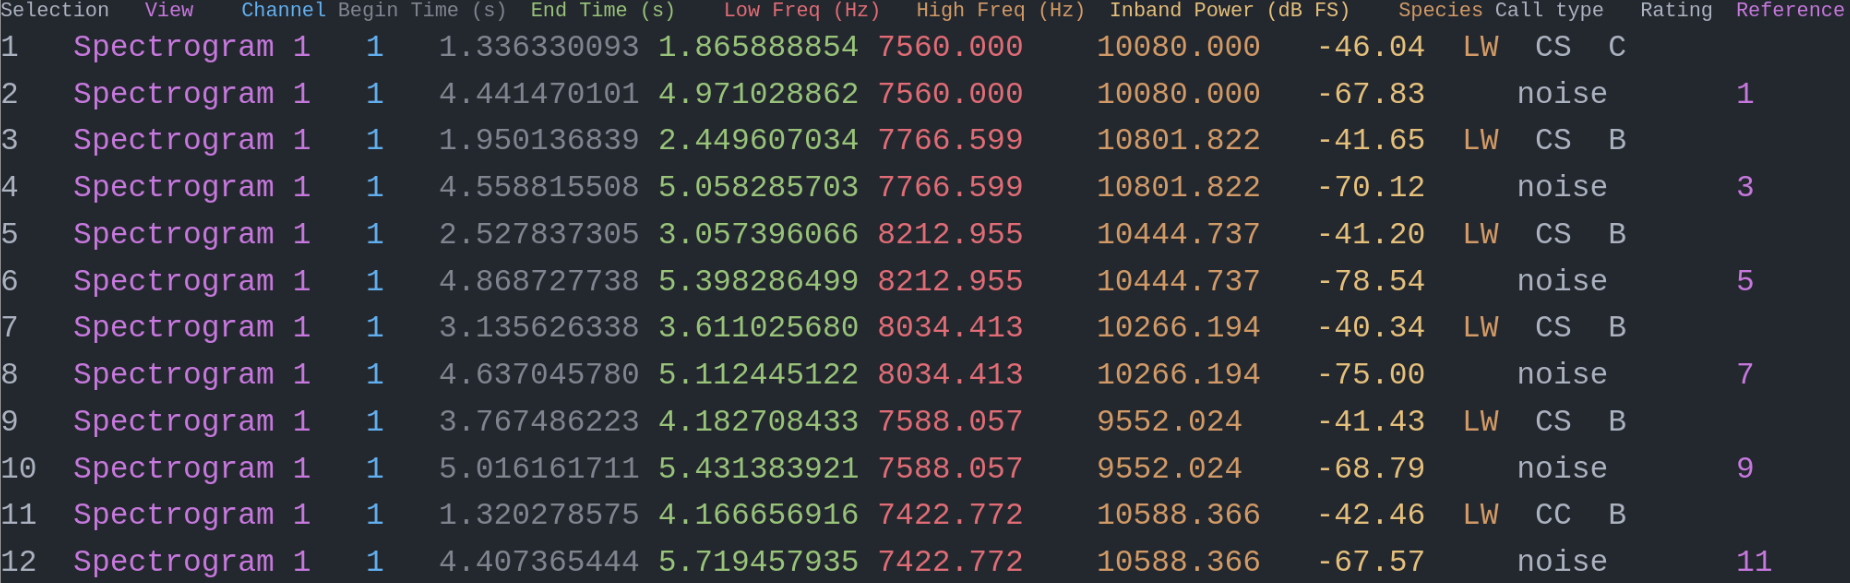
\includegraphics[width=0.95\textwidth]{figures/image4.png}
    \caption[Archivo de anotaciones de Raven]{Archivo de anotaciones de una grabación, con las columnas
        diferenciadas por color. El formato es un archivo de texto delimitado por
        tabulaciones que Raven lee y escribe directamente.}
    \label{fig:anotaciones-crudas}
\end{figure}

Las anotaciones se crean y editan sobre la grabación en Raven
(Figura~\ref{fig:raven}). El analista dibuja una región rectangular sobre el
espectrograma y el software deriva de ella el rango de frecuencias, los tiempos
de inicio y fin, y la amplitud. Las columnas de especie y tipo de llamada se
escriben a mano, y son justamente las que concentran los problemas descritos a
continuación.

\begin{figure}[htbp]
    \centering
    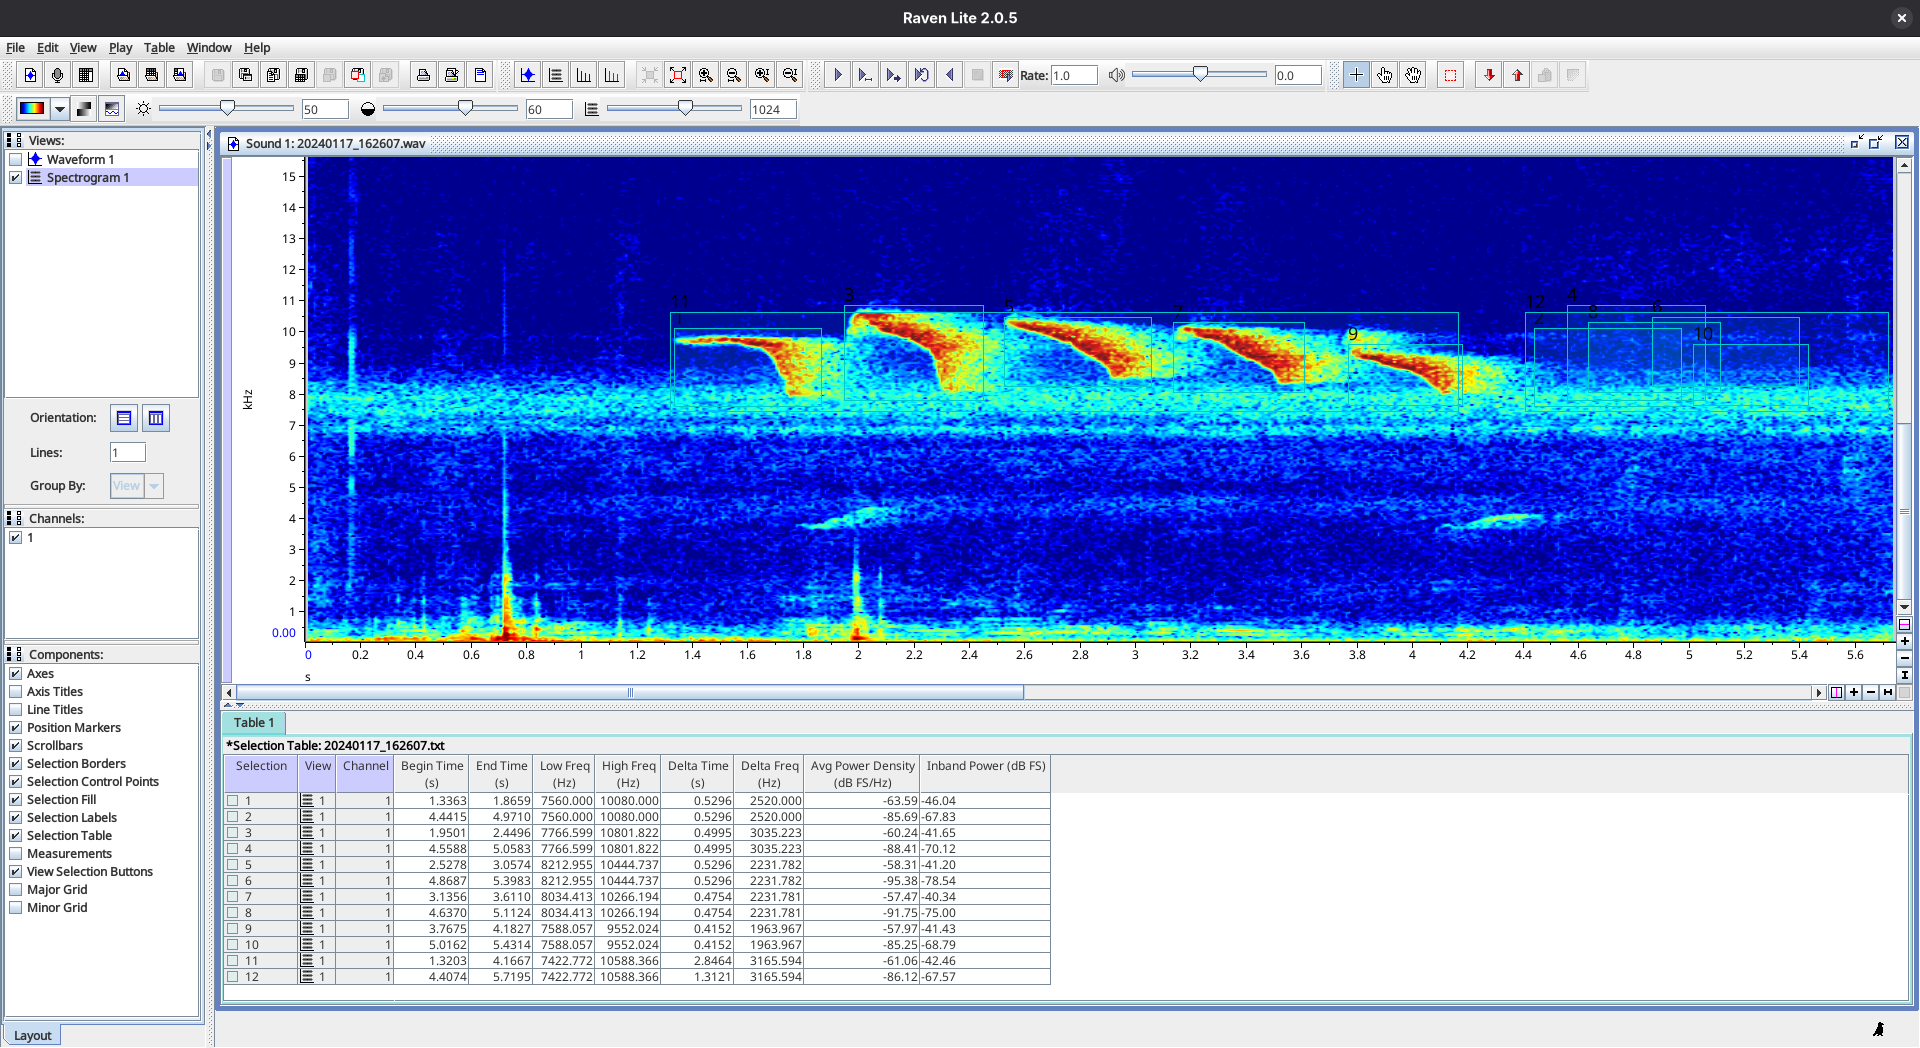
\includegraphics[width=0.92\textwidth]{figures/image5.png}
    \caption[Raven con una grabación anotada]{Raven durante el procesamiento de una grabación junto con sus
        anotaciones. Cada caja del espectrograma corresponde a una fila del archivo
        de la Figura~\ref{fig:anotaciones-crudas}.}
    \label{fig:raven}
\end{figure}

\subsection{Defectos detectados}

Un análisis exploratorio sobre el conjunto reveló cinco problemas que impiden
usar el material directamente para entrenamiento.

\rotulo{Inconsistencias de etiquetado.} Una misma clase aparece escrita de
múltiples formas. El prototipo inicial de este trabajo, restringido a la sílaba
de contacto del tamarino de Weddell, ya encontró en la columna de tipo de llamada
el conjunto de valores distintos
\texttt{\{CS, CS\char32, CS\char32\char32\char32\char32\char32\char32 A, contact
    syllable, CC, contact call, noise, noise\char32\char32\char32, noise|, noises,
    AA, A, B, C, TA\}}: cuatro grafías para una única clase, tres para el descarte
por ruido y un encabezado de columna que unas veces es \texttt{Call type} y otras
\texttt{Call Type}. Las Figuras~\ref{fig:etiquetas-especie}
y~\ref{fig:etiquetas-tipo} muestran los valores únicos encontrados en cada una de
las dos columnas manuales sobre el corpus completo.

\begin{figure}[htbp]
    \centering
    \begin{minipage}[t]{0.46\textwidth}
        \centering
        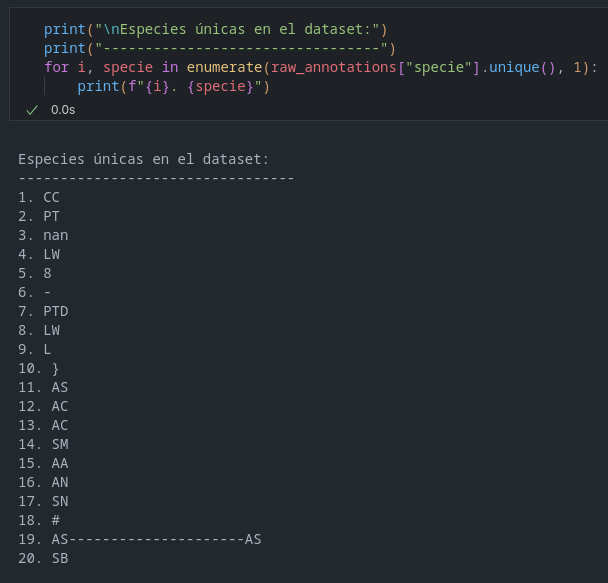
\includegraphics[width=\textwidth]{figures/image6.png}
        \caption{Etiquetas únicas encontradas en la columna de especie.}
        \label{fig:etiquetas-especie}
    \end{minipage}\hfill
    \begin{minipage}[t]{0.46\textwidth}
        \centering
        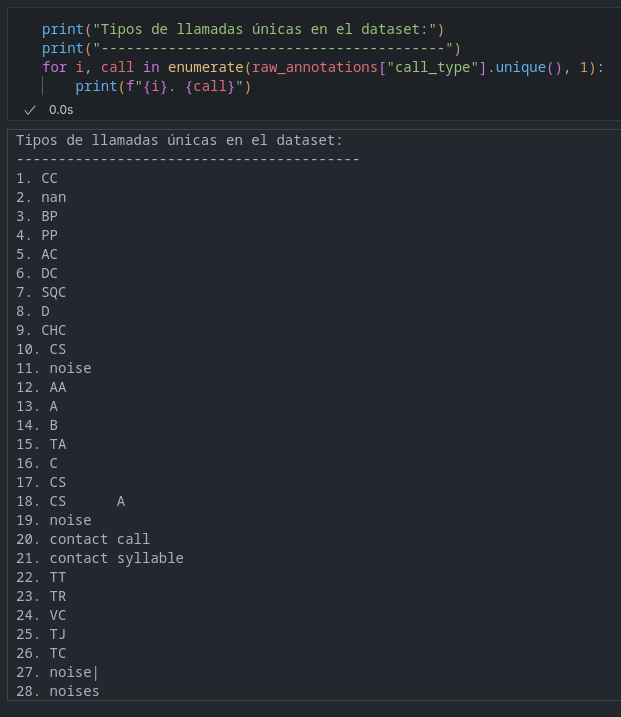
\includegraphics[width=\textwidth]{figures/image7.png}
        \caption{Etiquetas únicas encontradas en la columna de tipo de llamada.}
        \label{fig:etiquetas-tipo}
    \end{minipage}
\end{figure}

\rotulo{Integridad de los archivos.} La carga automatizada de las grabaciones
produce advertencias sobre archivos de audio dañados
(Figura~\ref{fig:advertencias}), que interrumpen el proceso si no se manejan de
forma explícita. La corrupción se manifiesta como bloques de ceros en la señal y
admite grados: la Figura~\ref{fig:corrupcion-leve} muestra un caso leve y la
Figura~\ref{fig:corrupcion-alta} uno en el que la mayor parte del archivo es
inutilizable. El origen probable son cortes durante la transferencia o fallos del
medio de almacenamiento.

\begin{figure}[htbp]
    \centering
    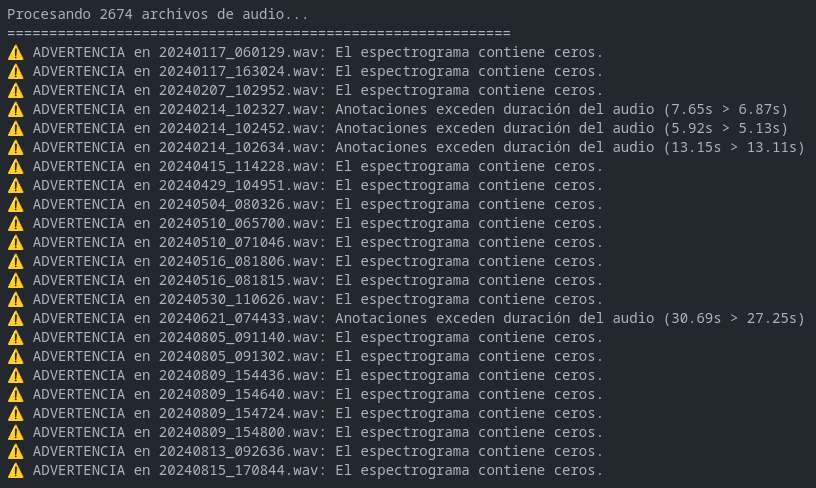
\includegraphics[width=0.85\textwidth]{figures/image8.png}
    \caption{Advertencias emitidas durante la carga automatizada de las
        grabaciones.}
    \label{fig:advertencias}
\end{figure}

\begin{figure}[htbp]
    \centering
    \begin{minipage}[t]{0.48\textwidth}
        \centering
        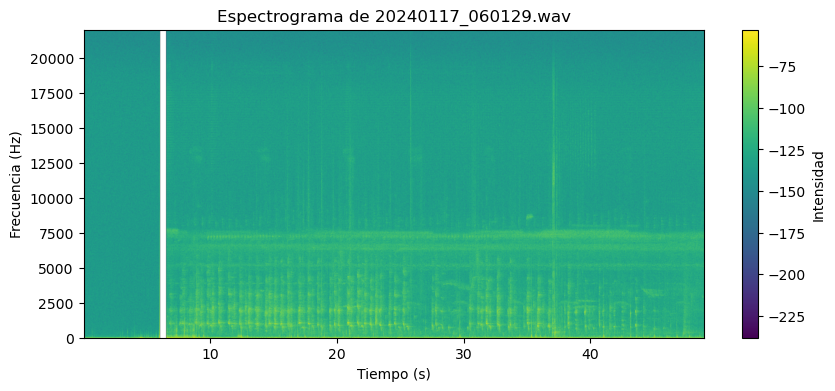
\includegraphics[width=\textwidth]{figures/image9.png}
        \caption{Grabación con corrupción leve}
        \label{fig:corrupcion-leve}
    \end{minipage}\hfill
    \begin{minipage}[t]{0.48\textwidth}
        \centering
        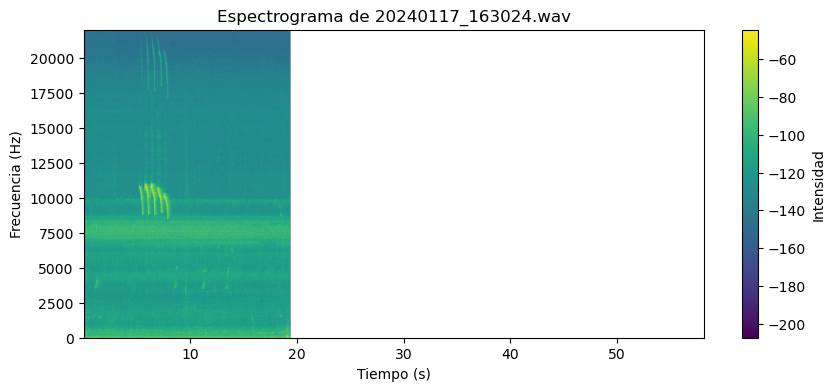
\includegraphics[width=\textwidth]{figures/image10.png}
        \caption{Grabación con corrupción severa}
        \label{fig:corrupcion-alta}
    \end{minipage}
\end{figure}

\rotulo{Discrepancias entre especie y carpeta.} La etiqueta de especie escrita en
la anotación no siempre coincide con el código de la carpeta contenedora, lo que
obliga a decidir cuál de las dos fuentes prevalece antes de consolidar nada.

\rotulo{Frecuencias por encima de Nyquist.} Algunas cajas declaran una frecuencia
superior mayor que el límite de Nyquist de la señal (22\,050\,Hz a 44,1\,kHz de
muestreo), un valor que no puede corresponder a energía observable en la
grabación.

\rotulo{Variabilidad en la unidad de análisis.} La granularidad de las
anotaciones no es uniforme. En unos casos el analista etiquetó sílabas
individuales y en otros delimitó una secuencia completa con una sola caja. No se
trata de un error de anotación sino de la manifestación directa del anidamiento
jerárquico de las unidades acústicas \citep{kershenbaum_acoustic_2016} descrito en el
Capítulo~\ref{cap:marco}; la subsección~\ref{sec:silabas} lo cuantifica.

\subsection{Composición del conjunto curado}

Tras aplicar el protocolo de la sección~\ref{sec:protocolo}, el conjunto queda en
\textbf{19\,042 anotaciones sobre ocho especies, repartidas en 57 pares
    distintos de especie y tipo de llamada}. De esos 57 pares, 41 pertenecen al
vocabulario declarado para el dominio y concentran 18\,714 anotaciones; los 16
restantes, que suman 328 registros (el 1,7\,\%), quedan fuera del vocabulario y se
marcan para revisión en lugar de descartarse en silencio. La
Tabla~\ref{tab:vocab-especie} resume el reparto por especie.

\begin{table}[htbp]
    \centering
    \small
    \begin{threeparttable}
        \caption{Composición del vocabulario curado por especie}
        \label{tab:vocab-especie}
        \begin{tabular}{@{}L{4.9cm}crrcr@{}}
            \toprule
                                           &               & \multicolumn{2}{c}{\textbf{En vocabulario}} & \multicolumn{2}{c}{\textbf{Experimento}}                                        \\
            \cmidrule(lr){3-4}\cmidrule(lr){5-6}
            \textbf{Especie}               & \textbf{Cód.} & \thead{Tipos}                               & \thead{Anotaciones}                      & \thead{Clases} & \thead{Anotaciones} \\
            \midrule
            \textit{Leontocebus weddelli}  & LW            & 11                                          & 4\,123                                   & 5              & 3\,492              \\
            \textit{Sapajus macrocephalus} & SM            & 8                                           & 3\,605                                   & 5              & 3\,395              \\
            \textit{Alouatta sara}         & AS            & 2                                           & 3\,310                                   & 2              & 3\,310              \\
            \textit{Ateles chamek}         & AC            & 6                                           & 3\,081                                   & 4              & 3\,017              \\
            \textit{Saimiri boliviensis}   & SB            & 5                                           & 2\,326                                   & 4              & 2\,277              \\
            \textit{Plecturocebus toppini} & PT            & 5                                           & 1\,156                                   & 2              & 1\,030              \\
            \textit{Aotus azarae}          & AA            & 3                                           & 1\,084                                   & 3              & 1\,084              \\
            \textit{Cebus cuscinus}        & CC            & 1                                           & 29                                       & 0              & N/D                 \\
            \midrule
            \textbf{Total}                 &               & \textbf{41}                                 & \textbf{18\,714}                         & \textbf{25}    & \textbf{17\,605}    \\
            \bottomrule
        \end{tabular}
        \begin{tablenotes}[flushleft]
            \footnotesize
            \item Las 328 anotaciones restantes hasta 19\,042 corresponden a los
            16 pares fuera de vocabulario, marcados para revisión.
            \item Los cuatro tipos de trino de LW cuentan como cuatro entradas
            del vocabulario y como una sola clase del experimento, por la fusión
            que justifica la sección~\ref{sec:seleccion}.
        \end{tablenotes}
    \end{threeparttable}
\end{table}

Dos propiedades de esa tabla gobiernan el resto del capítulo. La primera es que
\textbf{el vocabulario es desigual entre especies}: LW aporta once tipos de
llamada distintos sobre 4\,103 anotaciones, mientras que CC aporta un único tipo
con 29. La segunda es que \textbf{la distribución dentro de una especie es tan
    sesgada como la distribución entre especies}: en SM, el par \texttt{sm/acc}
cuenta con 8 anotaciones frente a las 2\,040 de \texttt{sm/cc}, un factor de
255$\times$ dentro de un mismo repertorio. La cola es
larga: los diez pares mayores concentran el 74\,\% de las 19\,042 anotaciones y
el resto se reparte hasta pares con una sola.

\begin{figure}[htbp]
    \centering
    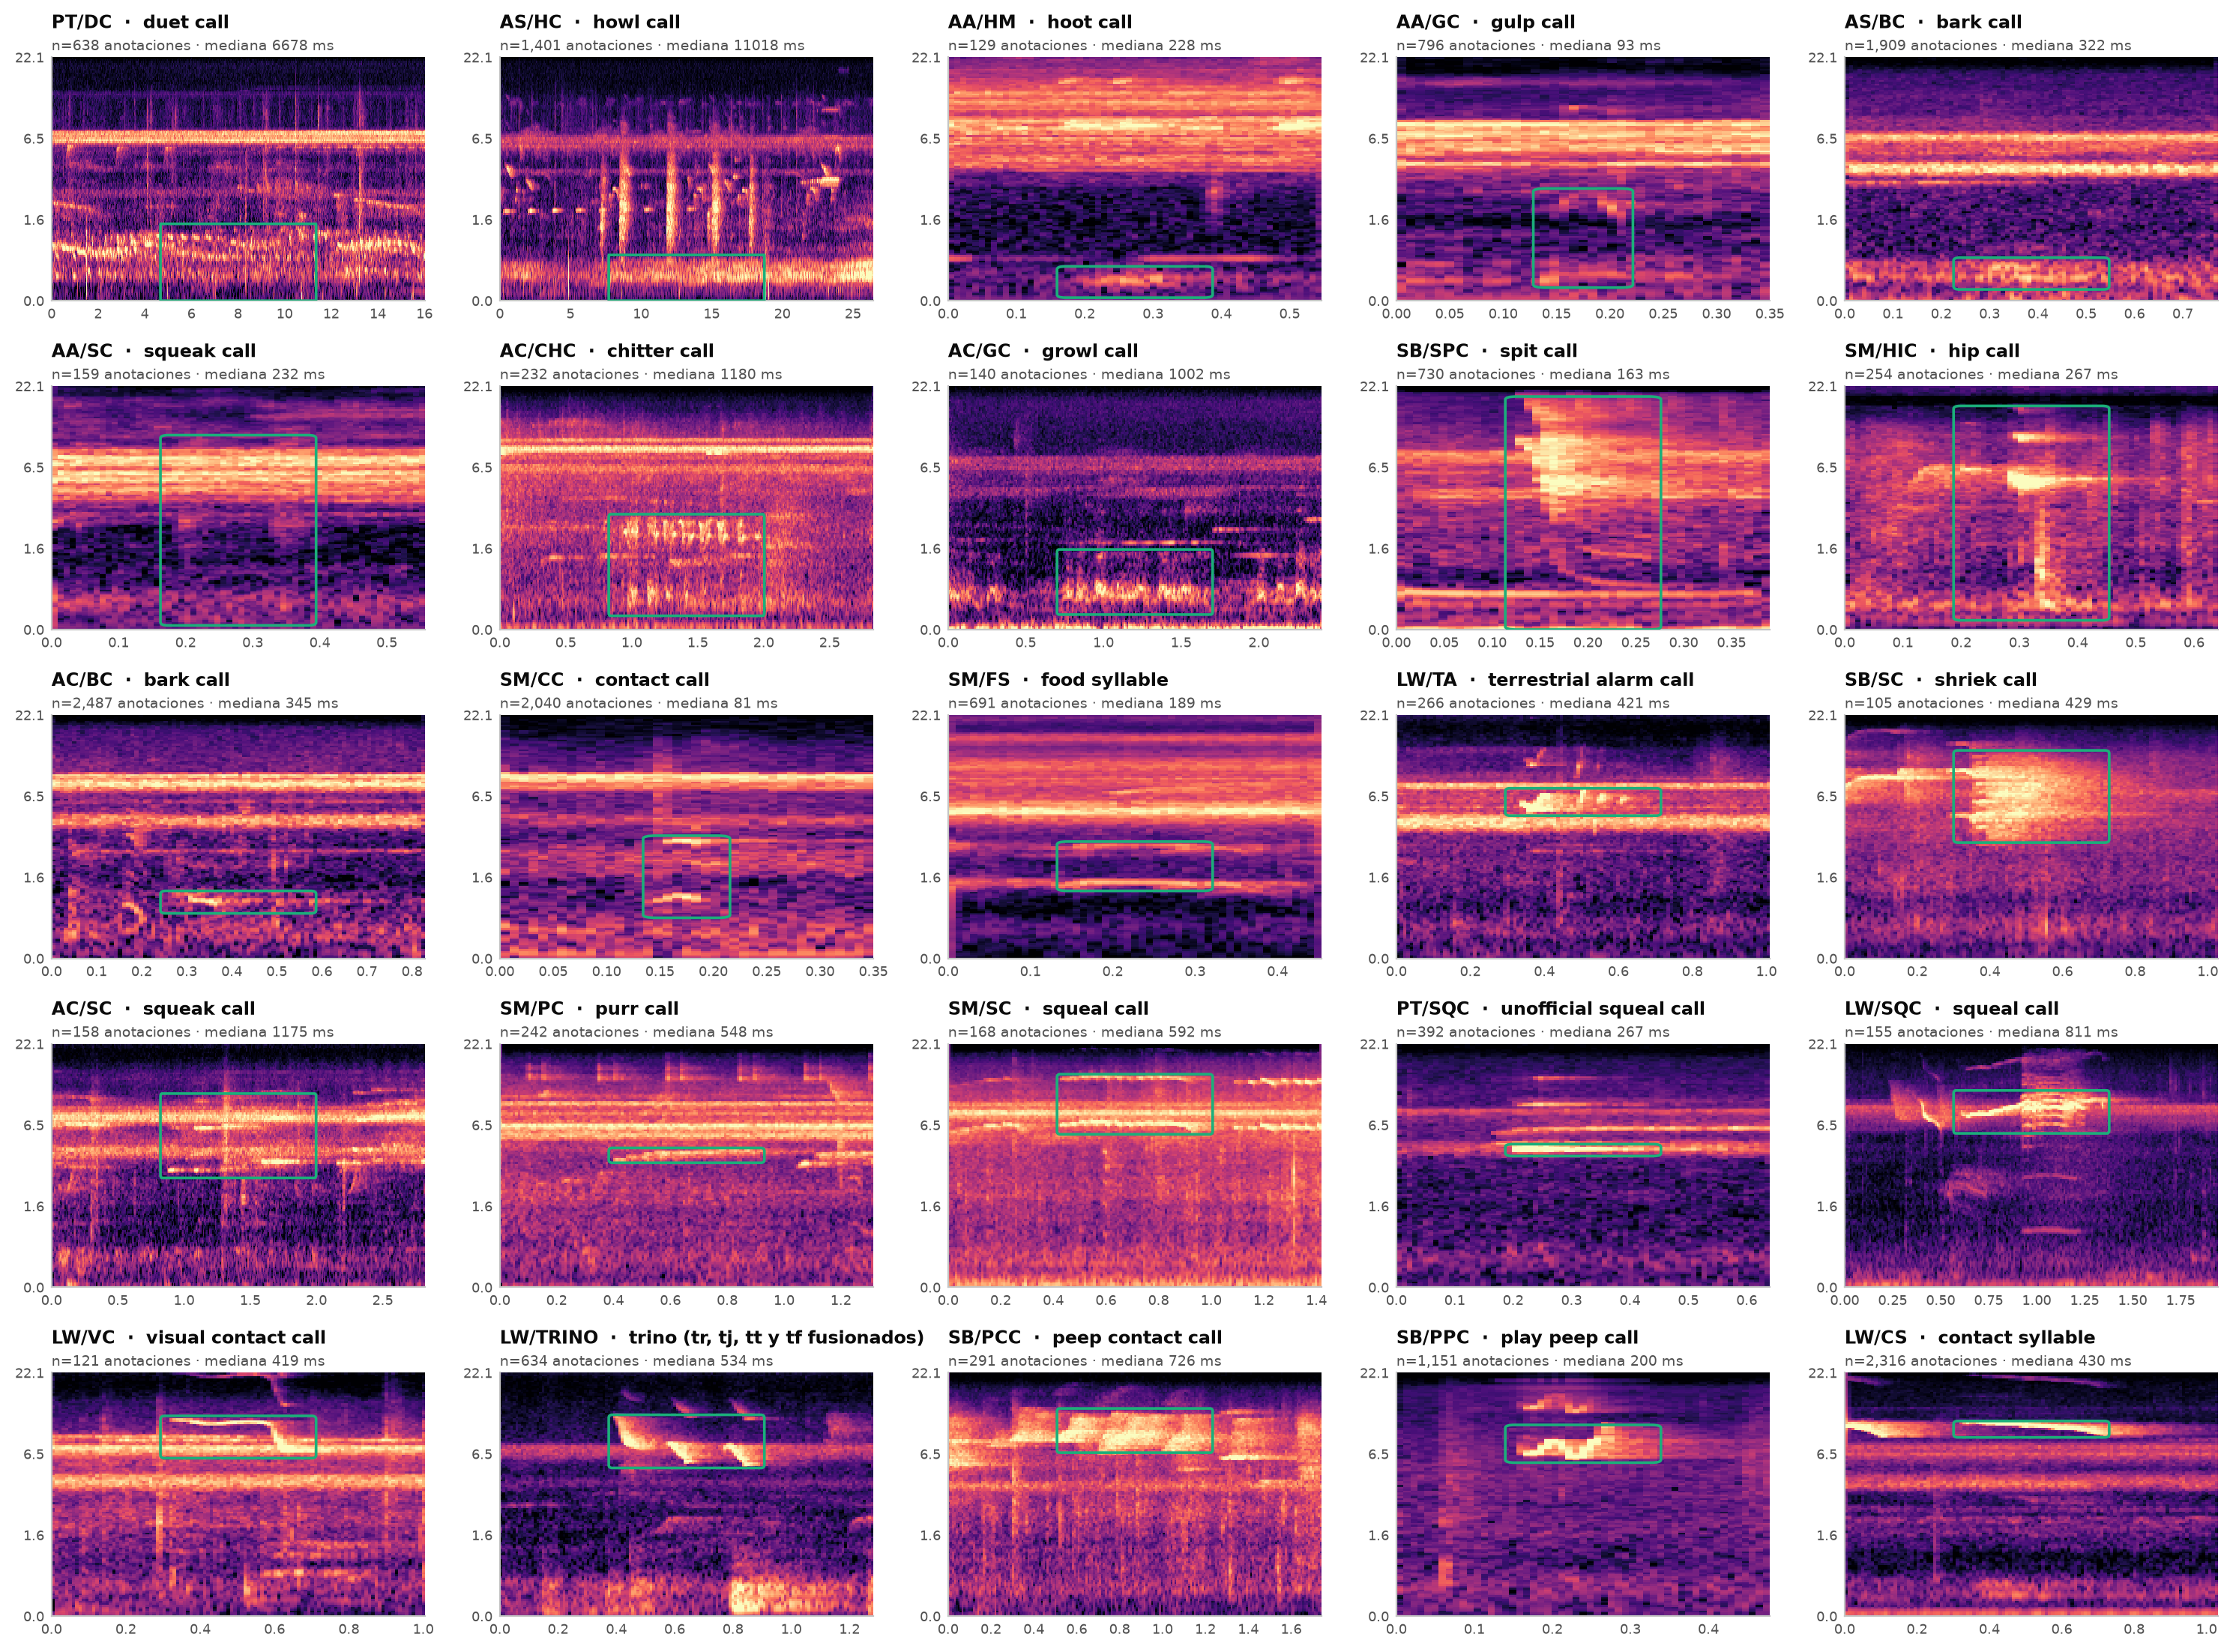
\includegraphics[width=\textwidth]{figures/call_gallery.png}
    \caption{Galería de llamadas.}
    \label{fig:call-gallery}
\end{figure}

\subsection{Geometría de los eventos}
\label{sec:geometria}

Las llamadas anotadas son extraordinariamente desiguales en tamaño, y ese hecho
condiciona todas las decisiones de diseño que siguen. La
Tabla~\ref{tab:geometria} lo mide sobre las 19\,042 anotaciones.

\begin{table}[htbp]
    \centering
    \caption{Variación de tamaño de las llamadas anotadas}
    \label{tab:geometria}
    \small
    \begin{tabular}{@{}L{4.0cm}rrr@{}}
        \toprule
                       & \thead{Mínimo} & \thead{Máximo} & \thead{Razón}           \\
        \midrule
        Duración       & 0,034\,s       & 73,3\,s        & \textbf{2\,134$\times$} \\
        Ancho de banda & 224\,Hz        & 21\,784\,Hz    & 97$\times$              \\
        \bottomrule
    \end{tabular}
\end{table}

La llamada más larga dura más de dos mil veces lo que la más corta. La magnitud
se aprecia mejor por comparación: en COCO, la colección de imágenes con la que se
evalúan habitualmente los detectores de objetos \citep{lin_2014}, los objetos
mayores superan a los menores en un factor de entre 10 y 100. El problema que
enfrenta este detector es, en ese eje, un orden de magnitud más severo que aquel
para el que se diseñaron las arquitecturas que hereda.

La consecuencia inmediata es que \textbf{ninguna longitud de ventana única sirve
    para todas las clases}: una ventana capaz de contener un aullido de 73\,s es
demasiado gruesa para resolver un chirrido de 34\,ms. La
sección~\ref{sec:ventaneo} documenta el compromiso adoptado y lo que cuesta.

La Figura~\ref{fig:class-geometry} sitúa cada clase en duración y en banda de
frecuencia, y hace visibles dos efectos a la vez.
Las \textbf{especies se separan en buena medida por banda}: AS ocupa
aproximadamente entre 25 y 1\,410\,Hz (percentiles 1 y 99), mientras que
\texttt{lw/cs} nunca aparece anotada por debajo de 3\,687\,Hz. Los \textbf{tipos
    de llamada dentro de una misma especie no se separan}: en LW, la familia de
trinos junto con \texttt{vc} y \texttt{cs} comparten banda y duración casi por
completo.

\begin{figure}[htbp]
    \centering
    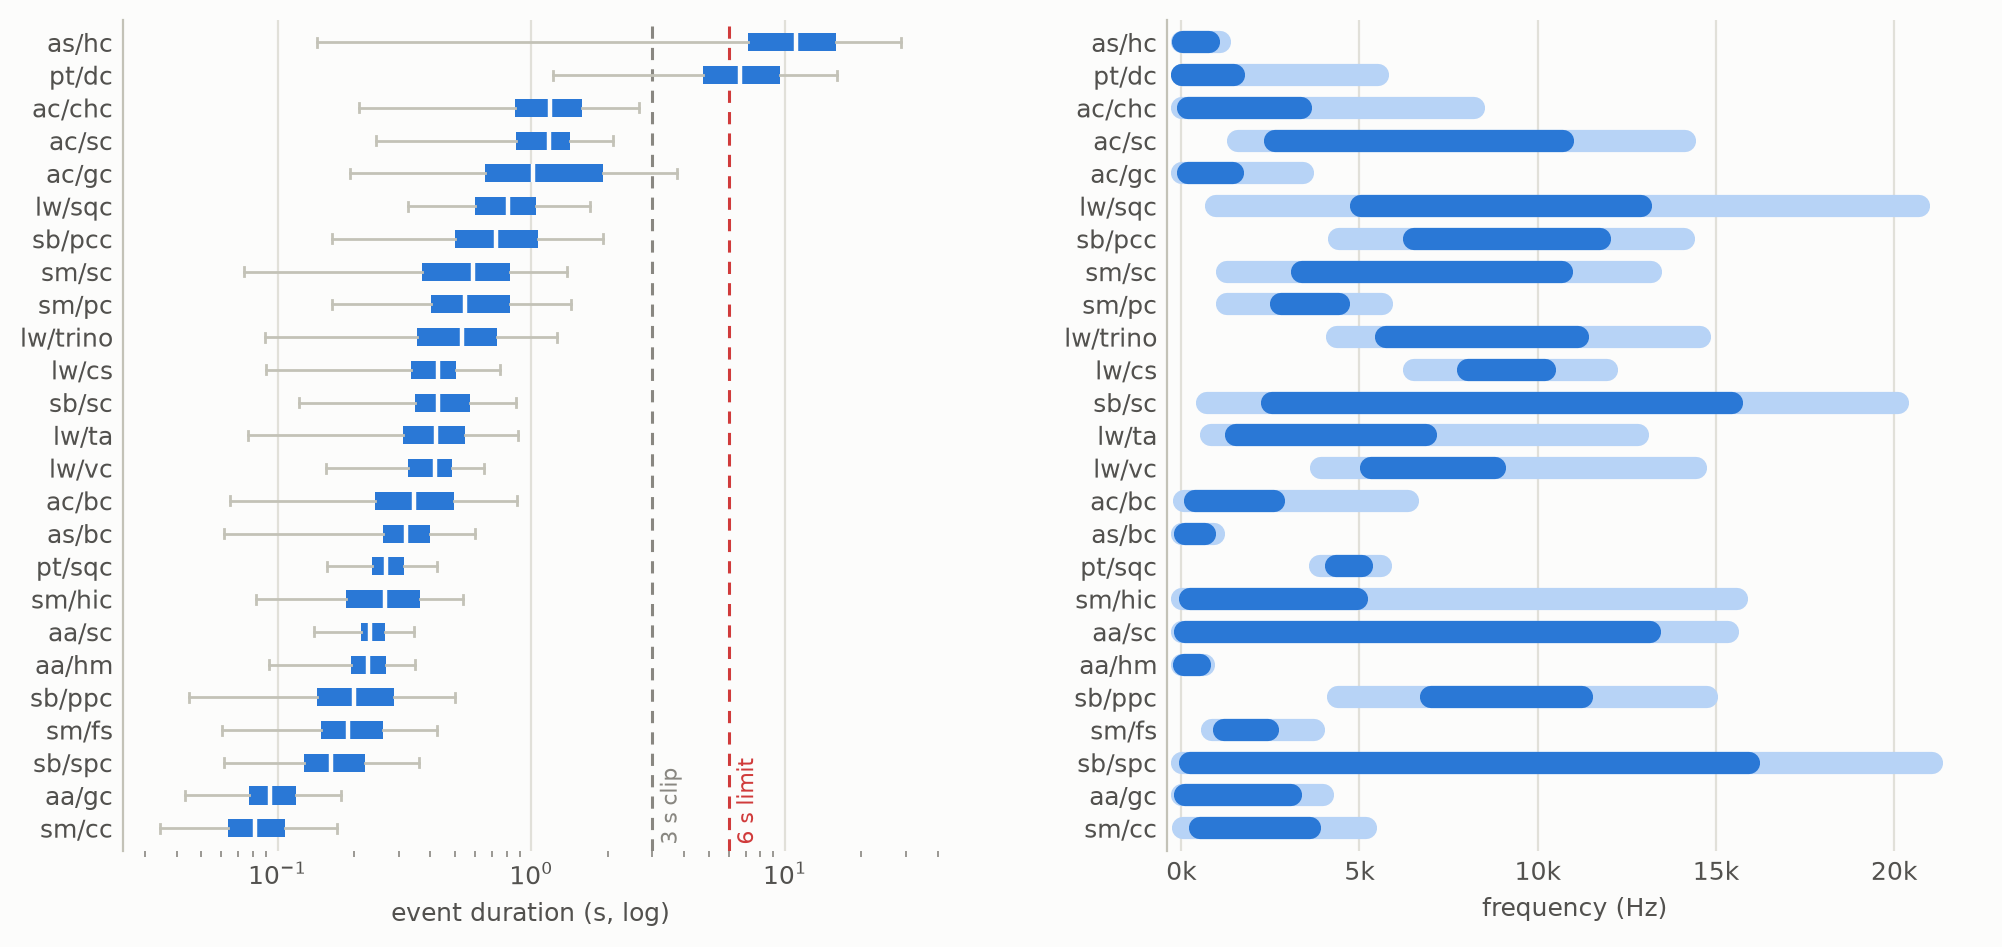
\includegraphics[width=\textwidth]{figures/class_geometry.png}
    \caption[Geometría de las clases]{Dónde vive cada clase en tiempo y en frecuencia. Las especies
        ocupan bandas distintas; los tipos de llamada de una misma especie se
        solapan casi por completo. La figura abarca los pares del vocabulario
        curado con suficientes anotaciones para caracterizarlos, un conjunto algo
        más amplio que las veinticinco clases del experimento
        (Tabla~\ref{tab:clases-experimento}).}
    \label{fig:class-geometry}
\end{figure}

Esa disociación tiene una consecuencia metodológica directa, y es la que sostiene
el protocolo de evaluación del Capítulo~\ref{cap:deteccion}: si la geometría
distingue especies pero no tipos de llamada, entonces \emph{localizar} y
\emph{etiquetar} son problemas de dificultad distinta y no deben puntuarse con
una sola cifra. De ahí que la detección se entrene de forma agnóstica a la clase
y la clasificación se evalúe por separado.

La Figura~\ref{fig:facets} desglosa la geometría par por par y revela un problema distinto del desbalance:
\texttt{ac/bc} (coeficiente de variación del ancho de banda 0,60) y
\texttt{sm/fs} (0,63) se parten cada uno en dos nubes claramente separadas en el
plano duración\,$\times$\,ancho de banda, mientras que \texttt{sb/ppc} (0,47) es
una única mancha difusa. Que una etiqueta cubra dos nubes disjuntas sugiere que
agrupa dos variantes de llamada que el vocabulario actual no distingue. Es un
hallazgo sobre el esquema de anotación, no sobre el modelo. Son, además, las
clases con peor \textit{recall} en la evaluación del
Capítulo~\ref{cap:deteccion}.

\begin{figure}[htbp]
    \centering
    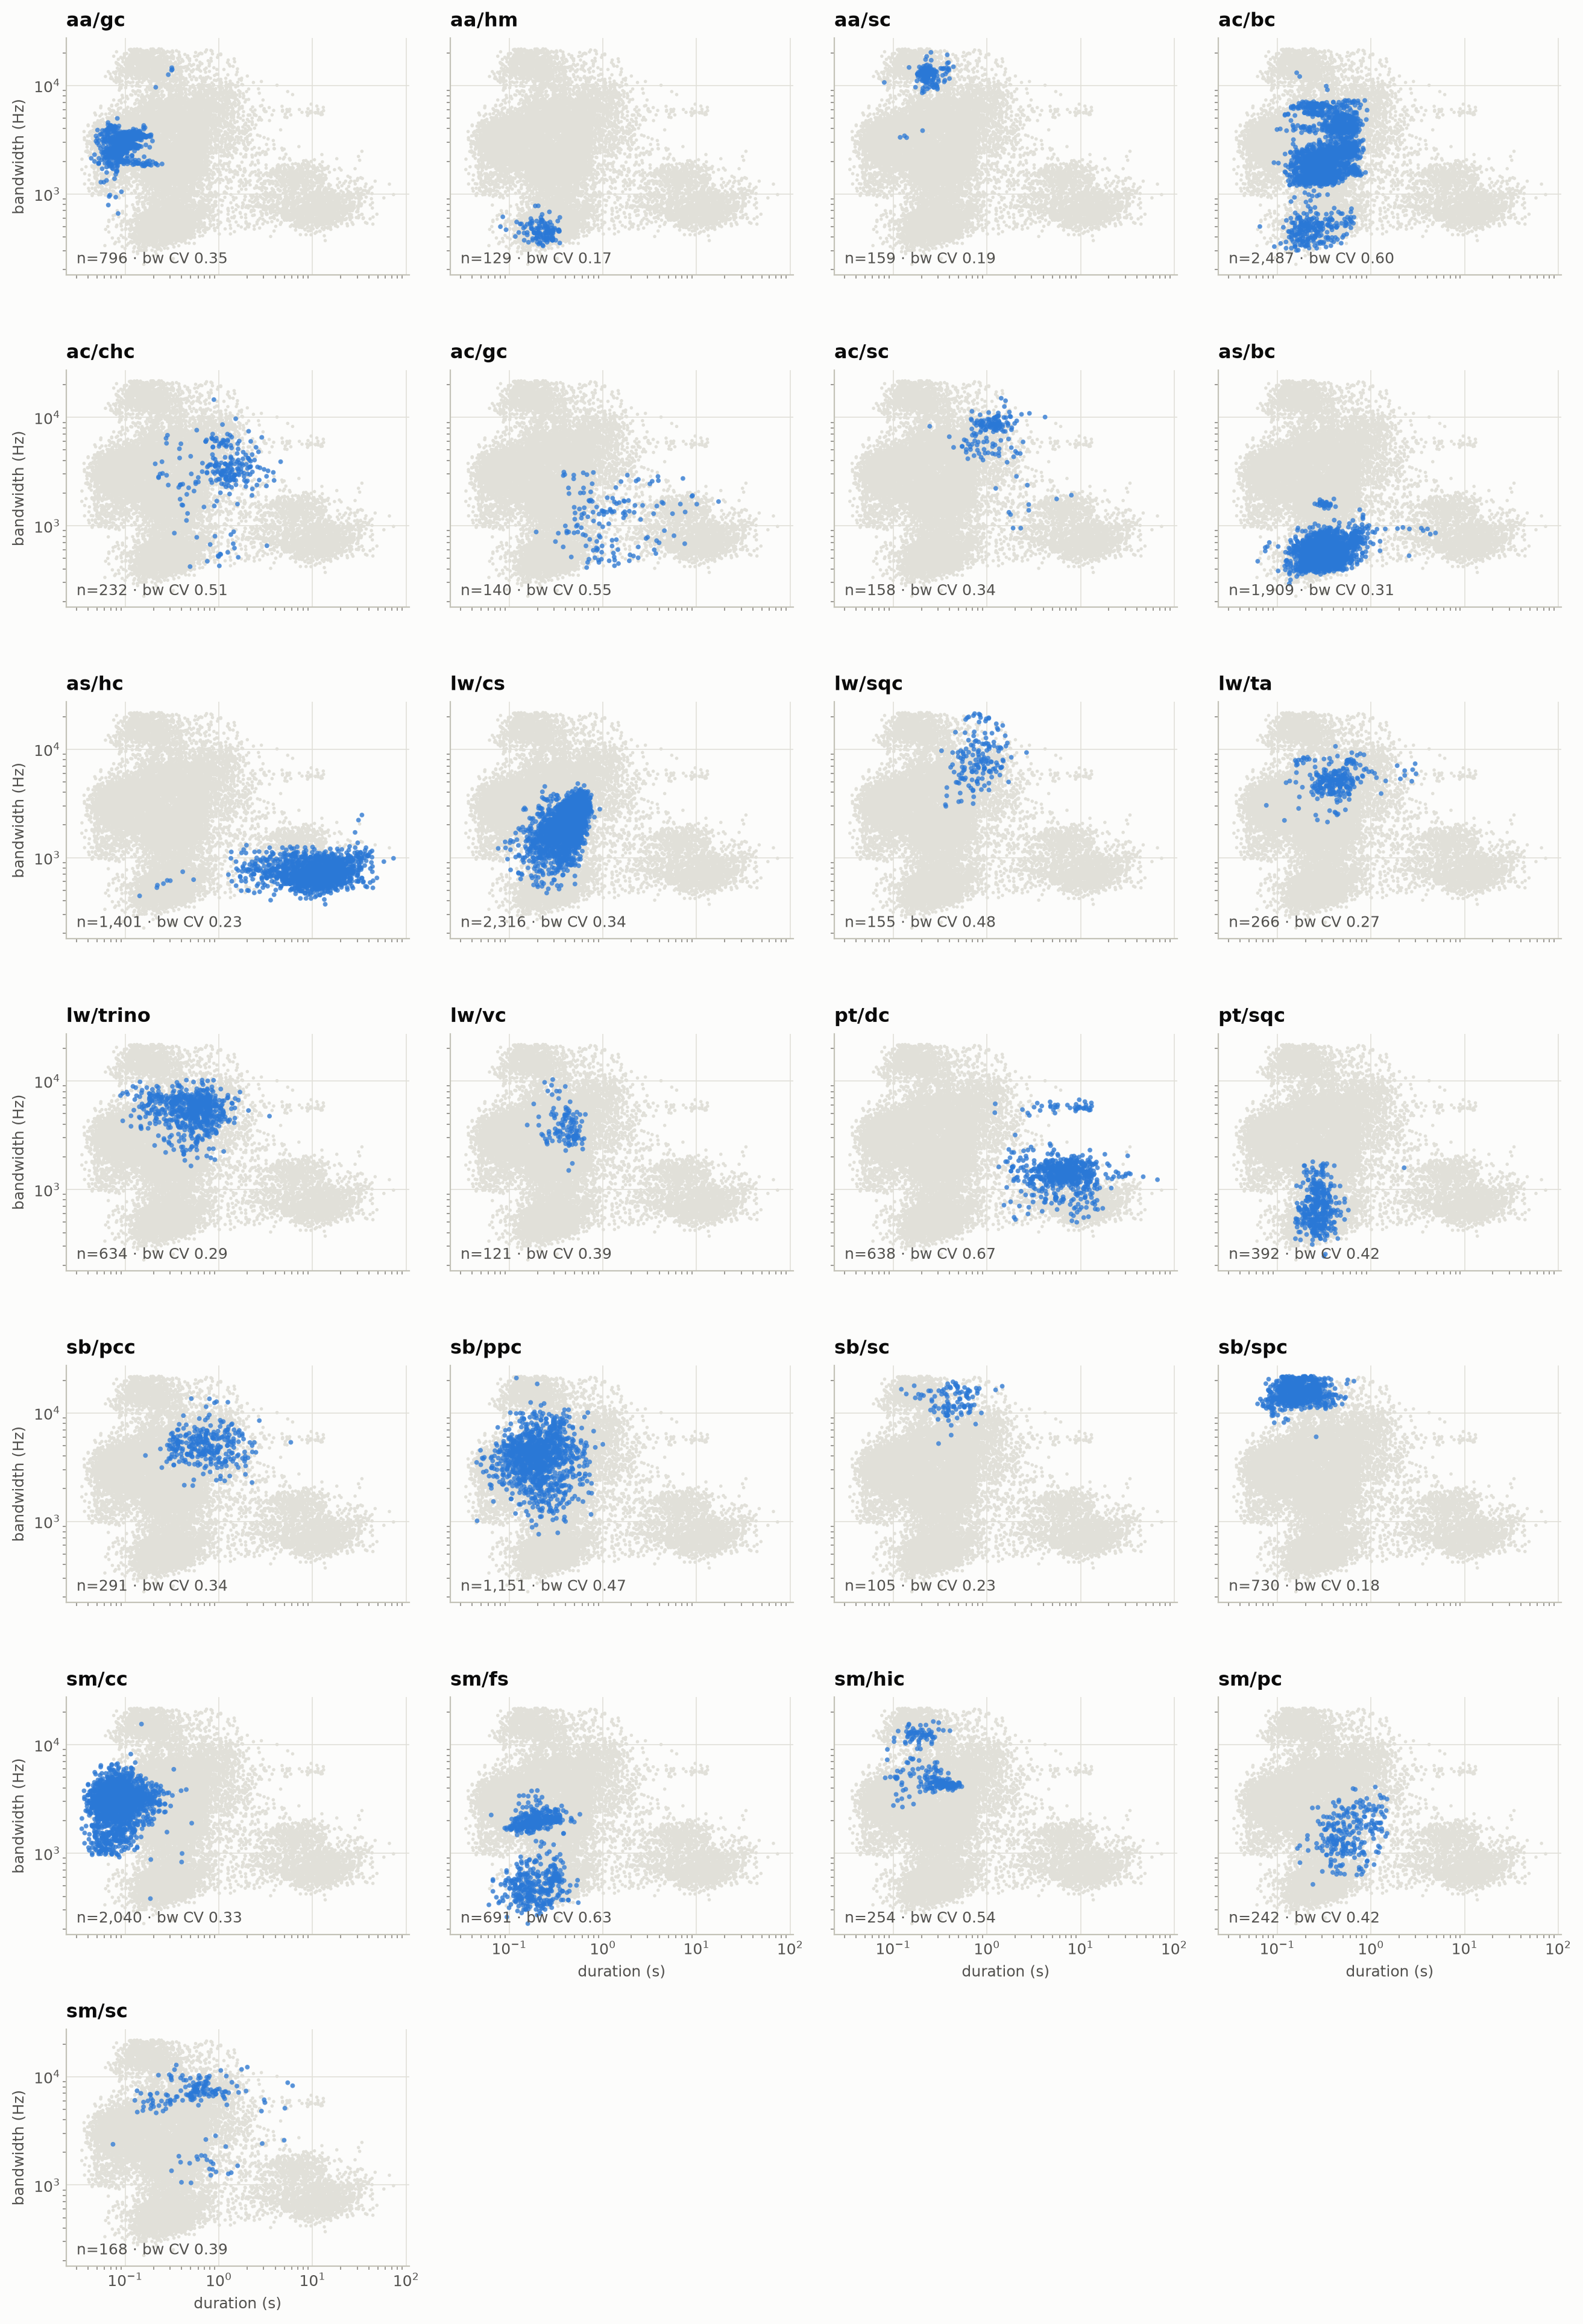
\includegraphics[height=0.80\textheight]{figures/class_geometry_facets.png}
    \caption[Duración frente a ancho de banda]{Duración frente a ancho de banda, un panel por par del
        vocabulario curado. En gris, todas las clases; en color, la del panel. Las
        nubes partidas de \texttt{ac/bc} y \texttt{sm/fs} indican una etiqueta
        única que cubre dos variantes de llamada.}
    \label{fig:facets}
\end{figure}

\subsection{Sílabas y frases}
\label{sec:silabas}

Una \emph{frase} es una secuencia de \emph{sílabas}, y los expertos anotan ambas:
el 94,2\,\% de las frases \texttt{lw/cc} contienen al menos una sílaba
\texttt{lw/cs}, y el 96,8\,\% de las frases \texttt{sm/fc} contienen una sílaba
\texttt{sm/fs}. El mismo tramo de audio lleva, por tanto, una caja grande y
varias cajas pequeñas dentro de ella.

El detector no puede representar esa relación. Devuelve una lista plana de cajas,
y el emparejamiento durante el entrenamiento asocia cada anotación verdadera con
exactamente una predicción, sin manera de expresar que ``esta caja contiene a
aquella''. Conservar ambos niveles equivaldría a pedir al modelo que informe dos
veces el mismo sonido, como si fueran dos eventos no relacionados superpuestos.
Es la consecuencia operativa del anidamiento jerárquico que
\citet{kershenbaum_acoustic_2016} describen como propiedad general de las unidades
acústicas animales: una secuencia de unidades puede ella misma considerarse una
unidad. Las dos clases de frase se excluyen, en consecuencia, antes del
entrenamiento.

\begin{figure}[htbp]
    \centering
    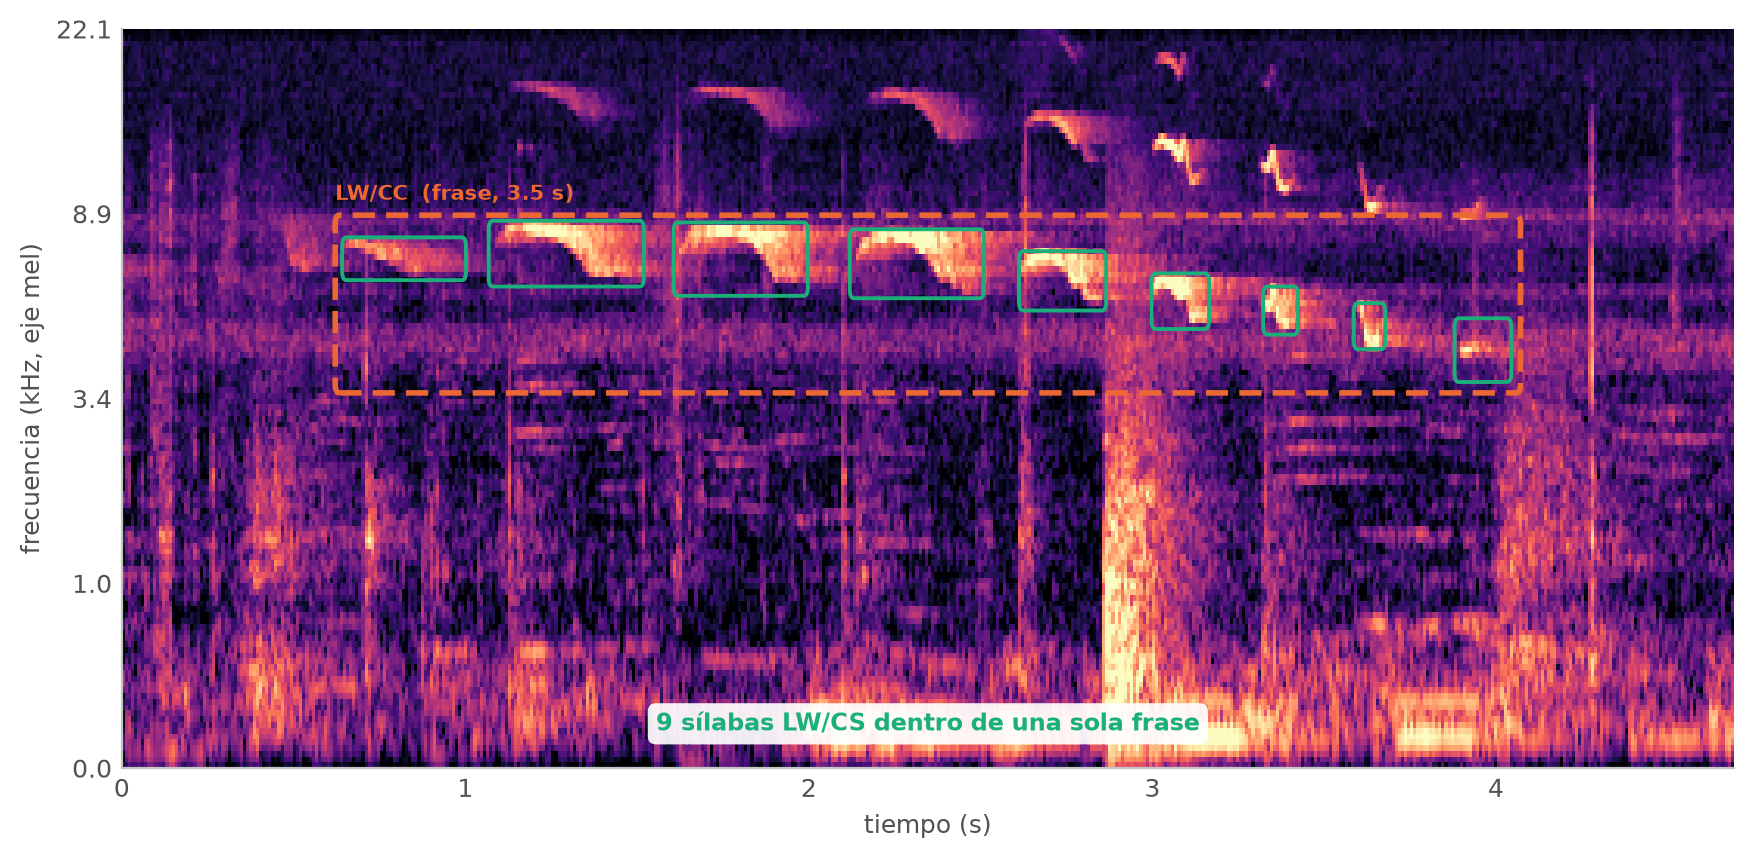
\includegraphics[width=0.92\textwidth]{figures/nesting_phrase.png}
    \caption{Anidamiento frase-sílaba.}
    \label{fig:nesting-phrase}
\end{figure}

\section{Protocolo de curación y estandarización (RE1.1)}
\label{sec:protocolo}

El protocolo se implementa como un \textit{pipeline} programático, no como una
corrección manual del material recibido. La distinción importa: un protocolo
ejecutable puede volver a aplicarse sobre los datos primarios cada vez que sus
reglas cambian, y deja registro de qué se descartó y por qué.

\begin{figure}[htbp]
    \centering
    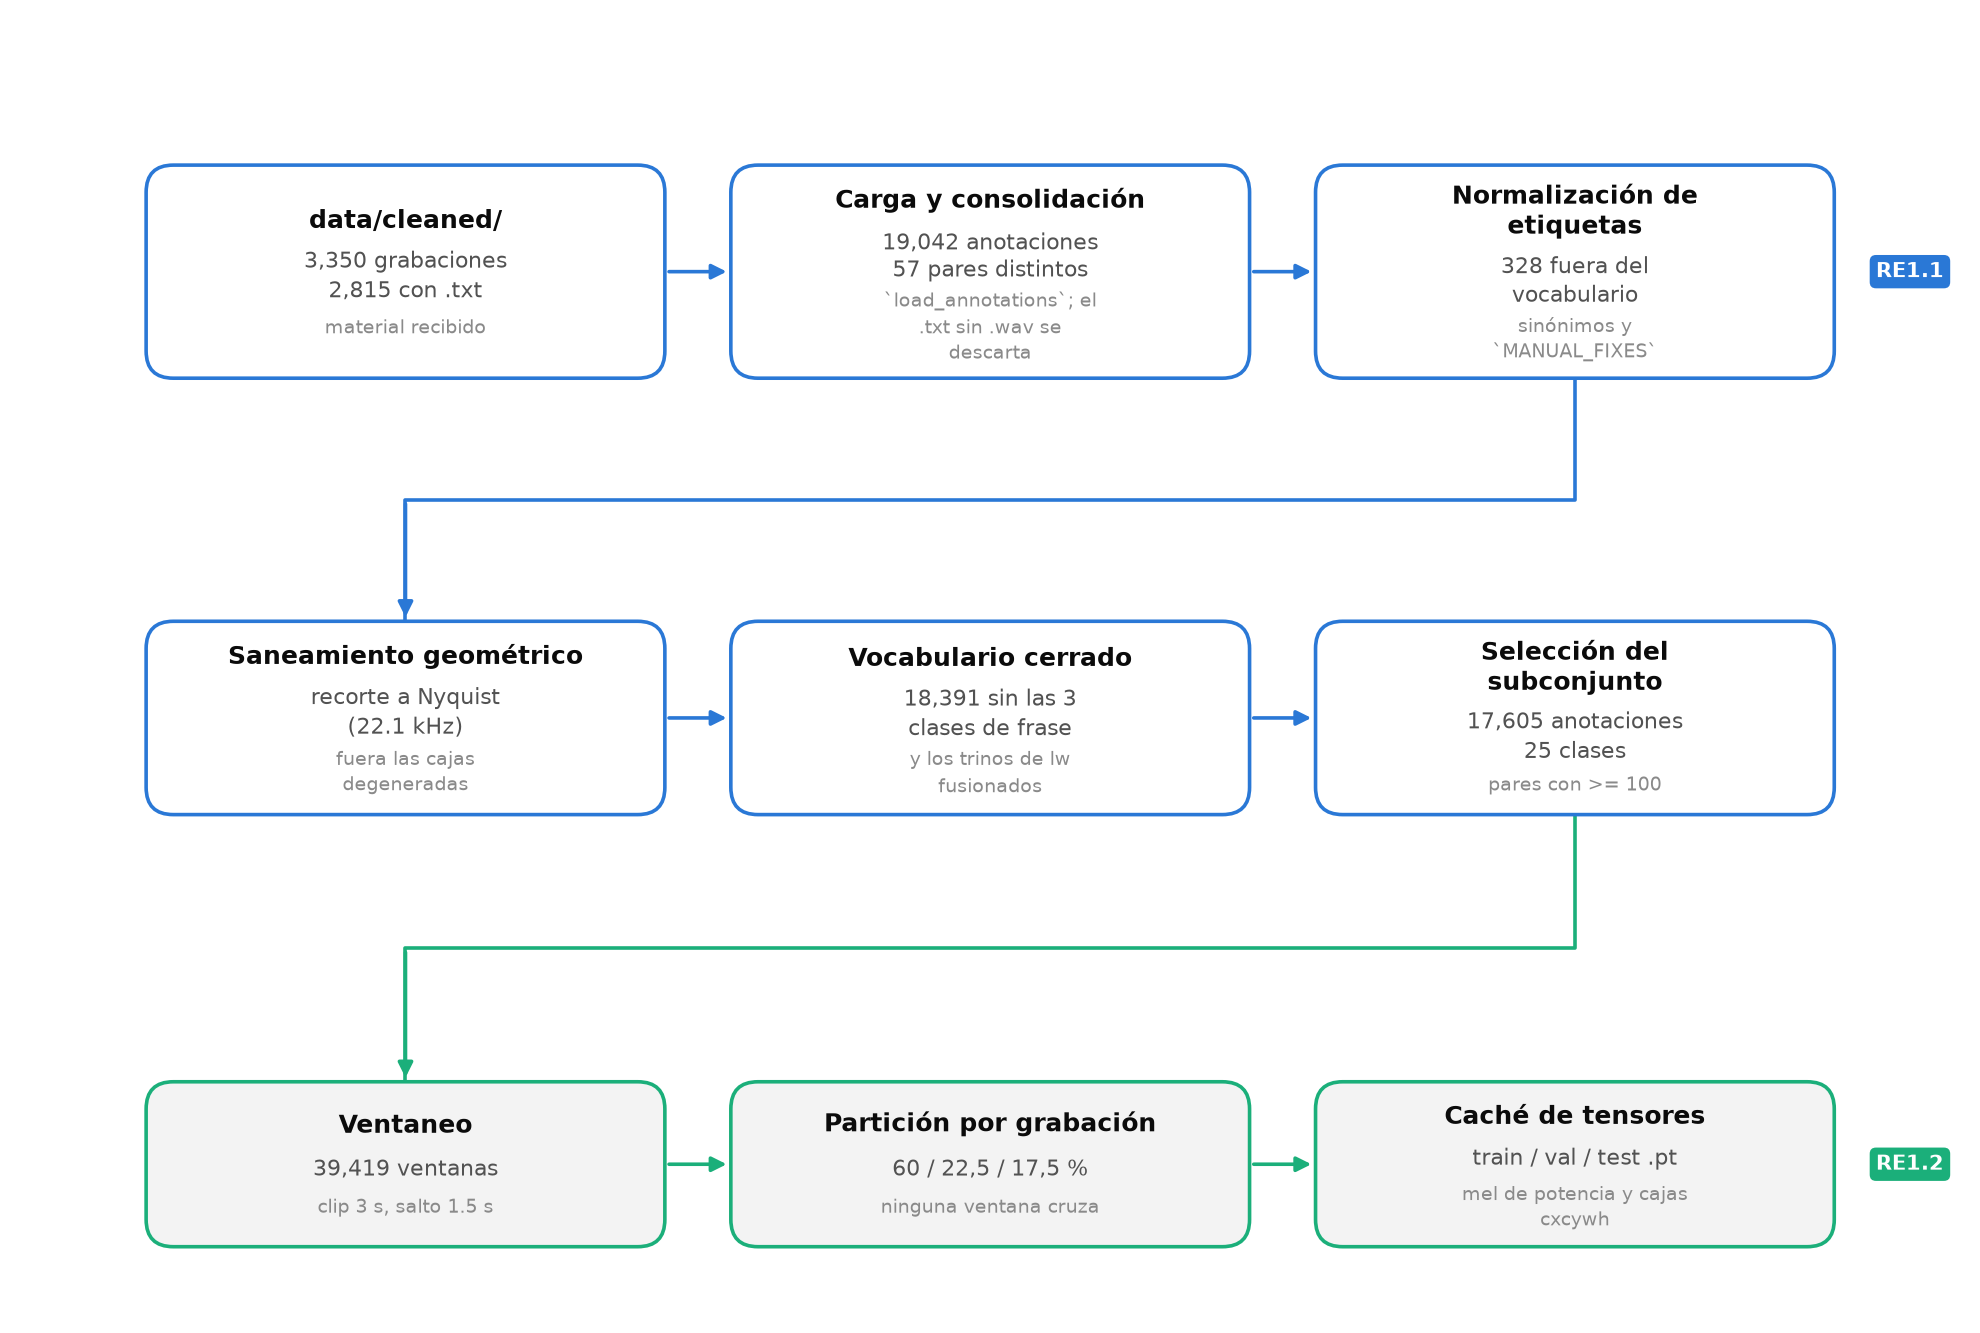
\includegraphics[width=\textwidth]{figures/curation_pipeline.png}
    \caption{Pipeline de curación.}
    \label{fig:curation-pipeline}
\end{figure}

\subsection{Carga y consolidación}

El primer paso recorre la estructura de directorios, lee cada archivo de
anotación y los unifica en una única tabla. Para cada archivo:

\begin{description}
    \item[Emparejamiento con el audio.] Solo se carga el archivo de anotación que
          tiene una grabación homónima junto a él. Un archivo de texto huérfano no
          aporta nada entrenable y su presencia suele indicar un error de transferencia.

    \item[Normalización de nombres de columna.] Los encabezados originales se
          convierten a un formato programático uniforme; \texttt{Begin Time (s)} pasa a
          \texttt{begin\_time\_s}, y de forma análoga el resto. Esto resuelve de una vez
          la alternancia entre \texttt{Call type} y \texttt{Call Type} observada en el
          material crudo.

    \item[Descarte de columnas no utilizadas.] Se eliminan las columnas de
          selección, vista, canal, referencia y desplazamiento de archivo, que
          corresponden al estado interno de Raven y no al evento.

    \item[Enriquecimiento con metadatos.] Se añaden la ruta de la grabación de
          origen y el directorio contenedor, que preserva la especie declarada por la
          organización del corpus.
\end{description}

Los errores de lectura se capturan y se registran, de modo que un archivo dañado
o un directorio vacío se omitan sin detener el proceso.

\subsection{Normalización de etiquetas}

Sobre la tabla consolidada se aplican, en este orden, las siguientes reglas.

\begin{description}
    \item[Normalización tipográfica.] Toda etiqueta se reduce a minúsculas y a
          caracteres alfanuméricos separados por guion bajo. Este único paso absorbe la
          mayoría de las variantes observadas, como espacios en blanco al final,
          mayúsculas inconsistentes y caracteres residuales, sin necesidad de
          enumerarlas.

    \item[Mapa de sinónimos.] Un diccionario explícito unifica las variantes que
          la normalización tipográfica no captura, por ser errores de escritura o
          abreviaturas alternativas y no diferencias de formato: \texttt{noises} a
          \texttt{noise}, \texttt{cs\_a} a \texttt{cs}, \texttt{whinnie} a
          \texttt{whc}, \texttt{tca} y \texttt{tac} a \texttt{ta}, \texttt{contact} a
          \texttt{cc}, \texttt{chcj} a \texttt{chc}, \texttt{php} a \texttt{phc},
          \texttt{sqr} a \texttt{sqc}, y \texttt{tc} a \texttt{tr}. Al mapa se suma, por
          especie, la traducción del nombre legible del tipo de llamada a su código
          \texttt{contact syllable} a \texttt{cs}, de modo que las anotaciones
          escritas en prosa converjan con las escritas en código.

    \item[Descarte de ruido.] Las anotaciones cuyo tipo de llamada, ya
          normalizado, es \texttt{noise} se eliminan: marcan la ausencia de evento, no
          un evento.

    \item[Corrección de pares imposibles.] Un pequeño conjunto de correcciones
          explícitas resuelve pares que no existen en el repertorio de la especie y
          cuya intención es inequívoca; por ejemplo, \texttt{aa/hc} se corrige a
          \texttt{aa/hm}, dado que AA no tiene llamada de aullido pero sí de ululato.
\end{description}

Ante una discrepancia entre la especie escrita en la anotación y el código de la
carpeta contenedora, prevalece la carpeta. El criterio no es arbitrario: el directorio es un dato estructural,
fijado una vez por sesión de campo, mientras que la columna de especie se teclea
en cada fila y es donde se observaron los errores de la
Figura~\ref{fig:etiquetas-especie}.

\subsection{Saneamiento geométrico}

Las coordenadas de la caja se validan de forma independiente de la etiqueta:

\begin{description}
    \item[Recorte a Nyquist.] La frecuencia superior se recorta a 22\,050\,Hz.
          Por encima de ese límite no hay energía observable en una señal muestreada a
          44,1\,kHz, de modo que un valor mayor es un error de anotación y no una
          propiedad del evento.

    \item[Descarte de cajas degeneradas.] Se eliminan las anotaciones de duración
          inferior a 10\,ms y las de ancho de banda nulo o negativo. Una caja sin área
          no define una región y no puede emparejarse con ninguna predicción.

    \item[Características derivadas.] Se calculan la duración y el ancho de banda
          de cada caja, que son las magnitudes sobre las que se construye el análisis de
          la sección~\ref{sec:geometria}.
\end{description}

\subsection{Vocabulario cerrado y selección del subconjunto}
\label{sec:seleccion}

El vocabulario admisible se declara de forma explícita como el conjunto de pares
(especie, tipo de llamada) válidos del dominio, no como aquello que aparezca en
los datos. Cerrar el vocabulario es la respuesta a la condición subyacente S2 del
árbol de problemas: las definiciones de unidad y las etiquetas semánticas varían
ampliamente entre investigadores, incluso dentro de un mismo grupo taxonómico
\citep{kershenbaum_acoustic_2016}, de modo que sin una lista fija la misma señal recibe
etiquetas distintas según quién la anote.

Los pares que caen fuera del vocabulario, 16 pares que suman 328 registros, no se
eliminan: se marcan con una bandera de revisión. La diferencia es deliberada. Un
par fuera de vocabulario puede ser un error de escritura no previsto o un tipo de
llamada legítimo aún no incorporado, y solo el equipo de investigación puede
distinguir uno de otro. Descartarlos en silencio destruiría esa evidencia.

Sobre el vocabulario se recorta el subconjunto de experimento en tres pasos:

\begin{enumerate}[nosep]
    \item \textbf{Exclusión por anidamiento.} Se retiran las dos clases de frase,
          \texttt{lw/cc} (517 anotaciones) y \texttt{sm/fc} (126), por la razón de la
          sección~\ref{sec:silabas}, y \texttt{sb/pcs} (8), que es la misma relación
          frase--sílaba dentro del repertorio de SB.

    \item \textbf{Fusión de los trinos de LW.} Los cuatro tipos de trino
          (\texttt{tr}, 333; \texttt{tj}, 164; \texttt{tt}, 106; \texttt{tf}, 31) se
          reúnen en una única clase \texttt{lw/trino} de 634 anotaciones. El motivo es
          geométrico y proviene de la sección~\ref{sec:geometria}: los cuatro comparten
          banda y duración casi por completo, de modo que mantenerlos separados obliga
          al detector a distinguir lo que la representación no distingue, y reparte
          entre cuatro etiquetas escasas un material que como clase única sí alcanza
          masa suficiente.

    \item \textbf{Umbral de frecuencia.} Se conservan los pares con al menos 100
          anotaciones. Por debajo de ese piso una clase no sostiene ni entrenamiento ni
          evaluación por clase: la más escasa que sobrevive, \texttt{sb/sc} con 105
          anotaciones, aporta apenas 126 cajas de entrenamiento.
\end{enumerate}

El resultado son las \textbf{25 clases y 17\,605 anotaciones} de la
Tabla~\ref{tab:clases-experimento}, el 92,5\,\% del conjunto curado, distribuidas
sobre siete de las ocho especies. El umbral deja fuera 26 pares con 786
anotaciones; de ellos, once pertenecen al vocabulario y suman 466 anotaciones,
entre los que está \texttt{cc/cc}: con 29 registros, la única llamada de CC no
alcanza el piso y esa especie queda fuera del experimento, aunque permanece en el
conjunto curado.

La elección del umbral en 100 y no más arriba es deliberada, y responde a una
tensión que conviene enunciar. Un umbral alto produce un experimento cómodo
—pocas clases, todas abundantes— a costa de dejar sin cubrir la mayor parte del
repertorio documentado: con el piso en 500 anotaciones sobrevivían diez clases,
el 74\,\% del material, y veintinueve tipos de llamada del vocabulario quedaban
sin usar. Bajar el piso a 100 cubre el 92,5\,\% del material y las cinco especies
que antes aportaban una sola clase pasan a aportar entre dos y cinco, al precio
de admitir clases cuyo desempeño estará limitado por su propia escasez y no por
la arquitectura. El Capítulo~\ref{cap:deteccion} lee los resultados por clase con
esa distinción presente, y la Figura~\ref{fig:annotations-per-pair} sitúa el
umbral sobre la distribución completa de pares.

\begin{figure}[htbp]
    \centering
    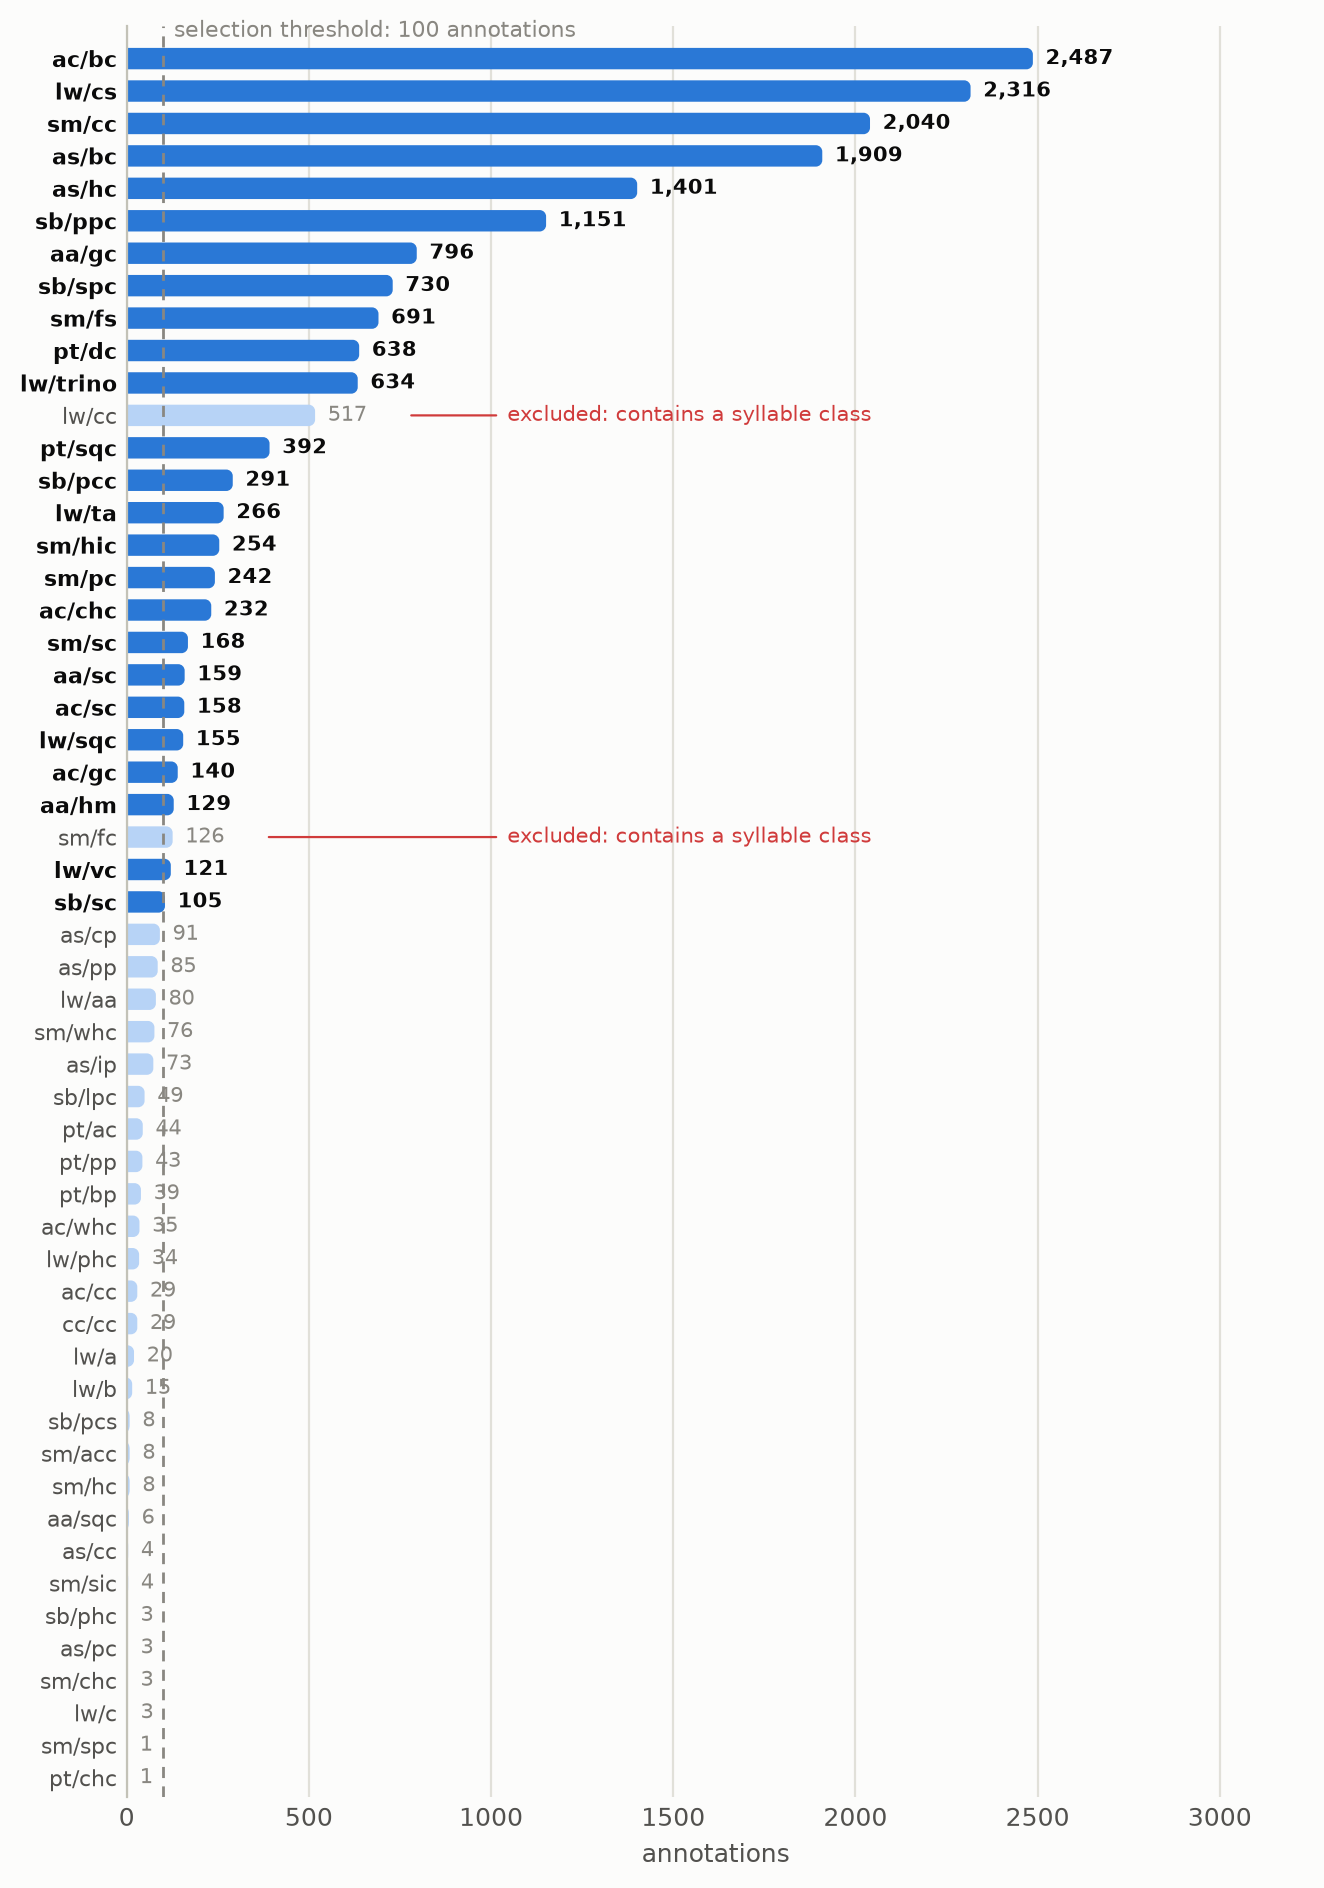
\includegraphics[height=0.80\textheight]{figures/annotations_per_pair.png}
    \caption[Anotaciones por par]{Anotaciones por par de especie y tipo de llamada. Las 25 clases por
        encima del umbral de 100 concentran el 92,5\,\% de las 19\,042 anotaciones;
        la cola larga llega hasta pares con una sola.}
    \label{fig:annotations-per-pair}
\end{figure}

\begin{table}[htbp]
    \centering
    \small
    \begin{threeparttable}
        \caption[Clases del subconjunto de experimento]{Clases del subconjunto de experimento y clases de frase excluidas}
        \label{tab:clases-experimento}
        \begin{tabular}{@{}L{2.2cm}L{5.2cm}rrL{2.6cm}@{}}
            \toprule
            \textbf{Clase}             & \textbf{Tipo de llamada}   & \thead{Anot.}    & \thead{Cajas\\(train)} & \textbf{Rol} \\
            \midrule
            \texttt{ac/bc}             & Ladrido                    & 2\,487           & 2\,886                 & Experimento  \\
            \texttt{lw/cs}             & Sílaba de contacto         & 2\,316           & 2\,706                 & Experimento  \\
            \texttt{sm/cc}             & Llamada de contacto        & 2\,040           & 2\,359                 & Experimento  \\
            \texttt{as/bc}             & Ladrido                    & 1\,909           & 2\,233                 & Experimento  \\
            \texttt{as/hc}             & Aullido                    & 1\,401           & 6\,933                 & Experimento  \\
            \texttt{sb/ppc}            & Llamada de juego           & 1\,151           & 1\,300                 & Experimento  \\
            \texttt{aa/gc}             & Llamada de trago           & 796              & 924                    & Experimento  \\
            \texttt{sb/spc}            & Llamada de escupido        & 730              & 860                    & Experimento  \\
            \texttt{sm/fs}             & Sílaba de comida           & 691              & 801                    & Experimento  \\
            \texttt{pt/dc}             & Dueto                      & 638              & 1\,950                 & Experimento  \\
            \texttt{lw/trino}          & Trino (fusión de 4 tipos)  & 634              & 739                    & Experimento  \\
            \texttt{pt/sqc}            & Chillido                   & 392              & 465                    & Experimento  \\
            \texttt{sb/pcc}            & Llamada de contacto (pío)  & 291              & 342                    & Experimento  \\
            \texttt{lw/ta}             & Alarma terrestre           & 266              & 312                    & Experimento  \\
            \texttt{sm/hic}            & Llamada \textit{hip}       & 254              & 295                    & Experimento  \\
            \texttt{sm/pc}             & Ronroneo                   & 242              & 283                    & Experimento  \\
            \texttt{ac/chc}            & Parloteo                   & 232              & 276                    & Experimento  \\
            \texttt{sm/sc}             & Chillido                   & 168              & 200                    & Experimento  \\
            \texttt{aa/sc}             & Chirrido                   & 159              & 183                    & Experimento  \\
            \texttt{ac/sc}             & Chirrido                   & 158              & 188                    & Experimento  \\
            \texttt{lw/sqc}            & Chillido                   & 155              & 182                    & Experimento  \\
            \texttt{ac/gc}             & Gruñido                    & 140              & 191                    & Experimento  \\
            \texttt{aa/hm}             & Ululato                    & 129              & 148                    & Experimento  \\
            \texttt{lw/vc}             & Contacto visual            & 121              & 140                    & Experimento  \\
            \texttt{sb/sc}             & Alarido                    & 105              & 126                    & Experimento  \\
            \midrule
            \texttt{lw/cc}             & Llamada de contacto        & 517              & ---                    & Excluida: contiene sílabas \\
            \texttt{sm/fc}             & Llamada de comida          & 126              & ---                    & Excluida: contiene sílabas \\
            \texttt{sb/pcs}            & Secuencia de píos          & 8                & ---                    & Excluida: contiene sílabas \\
            \midrule
            \textbf{Total experimento} &                            & \textbf{17\,605} & \textbf{27\,022}       &              \\
            \bottomrule
        \end{tabular}
        \begin{tablenotes}[flushleft]
            \footnotesize
            \item Las tres clases de frase se retiran por anidamiento
            (sección~\ref{sec:silabas}), no por escasez: \texttt{lw/cc} supera
            holgadamente el umbral y habría entrado al experimento.
            \item La columna de cajas cuenta ventanas de 3\,s de la partición de
            entrenamiento, no anotaciones. Las dos cifras no son proporcionales:
            \texttt{as/hc} y \texttt{pt/dc} multiplican su material porque cada
            llamada larga atraviesa varias ventanas
            (sección~\ref{sec:ventaneo}), y son las dos únicas clases donde eso
            ocurre.
        \end{tablenotes}
    \end{threeparttable}
\end{table}

\section{Particionado y ventaneo (RE1.2)}
\label{sec:ventaneo}

\subsection{Partición por archivo de grabación}

El conjunto se divide en entrenamiento, validación y prueba en proporción
60/22,5/17,5 de cajas por clase, con semilla fijada para que la partición sea
reproducible. La asignación es golosa y recorre las clases de la más rara a la
más común, de modo que el reparto de las clases escasas se decide primero y no
queda como residuo del de las abundantes. El resultado son 21\,966 ventanas de
entrenamiento, 9\,446 de validación y 8\,007 de prueba, con 27\,022, 10\,090 y
7\,985 cajas anotadas respectivamente. La división
se hace \textbf{por archivo de grabación}: todas las anotaciones de una misma
grabación caen en la misma partición, y ninguna ventana cruza particiones.

La alternativa de repartir anotaciones o ventanas sueltas no es un descuido
hipotético. El prototipo inicial de este trabajo la cometió: barajaba los clips
de 0,5\,s y los repartía por índice, con lo que dos ventanas solapadas
procedentes de la misma anotación podían quedar una en entrenamiento y otra en
prueba. Sobre esa partición el clasificador alcanzaba un 99\,\% de exactitud, una
cifra que no medía generalización sino memoria: el 91,2\,\% de los clips eran
negativos, de modo que un predictor constante ``sin llamada'' ya obtenía 91,2\,\%.
Dado que la variación en las etiquetas fuertes afecta por sí sola a la evaluación
\citep{koga_lead_2024}, no añadir además fuga de datos es la condición mínima
para que las cifras resulten interpretables.

La Tabla~\ref{tab:split} recoge la composición resultante.

\begin{table}[htbp]
    \centering
    \small
    \begin{threeparttable}
        \caption{Composición de las particiones tras el ventaneo}
        \label{tab:split}
        \begin{tabular}{@{}L{3.2cm}rrr@{}}
            \toprule
            \textbf{Partición} & \thead{Grabaciones} & \thead{Ventanas} & \thead{Cajas}    \\
            \midrule
            Entrenamiento      & 1\,166              & 8\,022           & 16\,674          \\
            Validación         & 166                 & 1\,043           & 2\,183           \\
            Prueba             & 335                 & 2\,490           & 5\,343           \\
            \midrule
            \textbf{Total}     & \textbf{1\,667}     & \textbf{11\,555} & \textbf{24\,200} \\
            \bottomrule
        \end{tabular}
        \begin{tablenotes}[flushleft]
            \footnotesize
            \item Hay más cajas que anotaciones porque una misma anotación puede
            caer en dos ventanas consecutivas: la ventana de 3\,s avanza 1,5\,s.
        \end{tablenotes}
    \end{threeparttable}
\end{table}

El balance entre clases se conserva a lo largo de las tres particiones, con un
rango de cajas de entrenamiento que va de 3\,273 para \texttt{lw/cs} a 320 para
\texttt{as/hc}. Ese último número llama la
atención: \texttt{as/hc} tiene 1\,400 anotaciones en la
Tabla~\ref{tab:clases-experimento} y, sin embargo, aporta menos cajas que clases
con la mitad de anotaciones. La razón es estructural y se documenta a
continuación.


\begin{figure}[htbp]
    \centering
    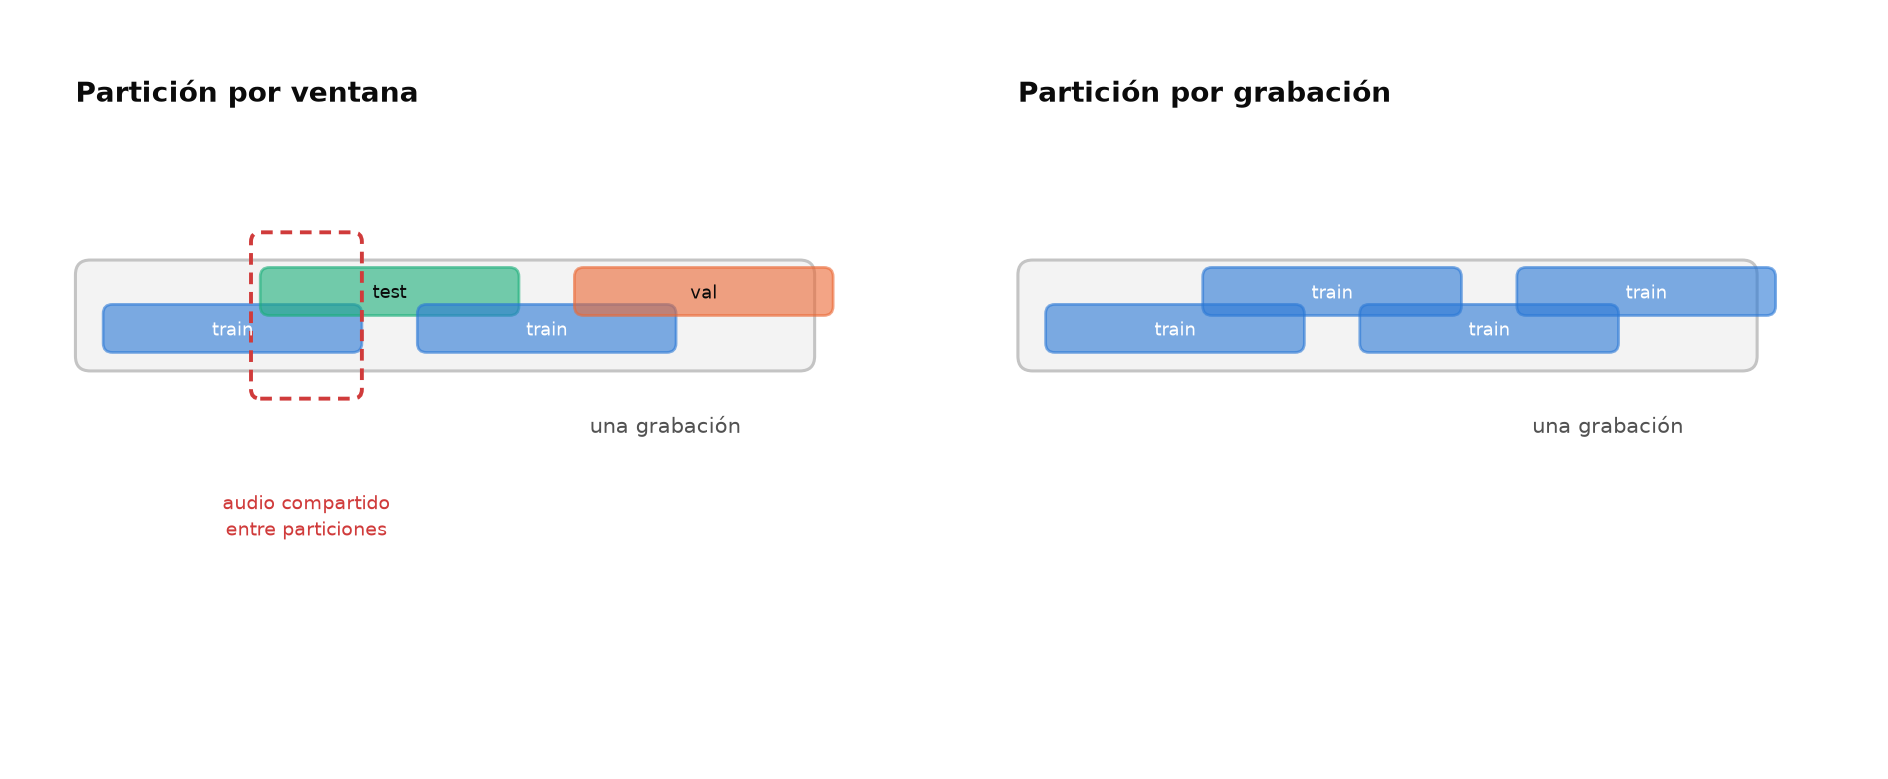
\includegraphics[width=\textwidth]{figures/split_by_recording.png}
    \caption{Partición por grabación.}
    \label{fig:split-by-recording}
\end{figure}

\subsection{El ventaneo y lo que le cuesta a las llamadas largas}

Las grabaciones tienen duración variable y el detector consume entradas de tamaño
fijo, de modo que cada grabación se segmenta en ventanas de 3\,s que avanzan
1,5\,s. La regla de asignación no compara el solapamiento contra la duración del
evento sino contra su \emph{parte visible}, definida como el mínimo entre la
duración del evento y la longitud de la ventana: una anotación entra en una
ventana si el solapamiento cubre al menos la mitad de esa parte visible.

El detalle no es menor. Comparar contra la duración completa dejaría
\textbf{inalcanzable a todo evento de más de 6\,s}, porque no existe posición de
la ventana en la que quepa la mitad de un aullido de 30\,s; con el criterio de
parte visible, en cambio, ese aullido entra en toda ventana que caiga dentro de
él. Ninguna anotación del subconjunto de experimento queda sin ventana.

Lo que el ventaneo cobra es otra cosa, y la Tabla~\ref{tab:ventaneo-largos} la
mide: las llamadas largas se \textbf{fragmentan}. Cada evento se reparte, en
promedio, entre 2,6 ventanas —consecuencia directa del salto de 1,5\,s, que hace
que casi todo evento breve aparezca en dos—, pero \texttt{as/hc} se reparte entre
8,2 y \texttt{pt/dc} entre 5,1. El aullido de \texttt{as/hc}, con 1\,401
anotaciones, aporta 11\,557 cajas: el 26\,\% de todas las cajas del conjunto
derivado provienen del 8\,\% de las anotaciones. Y esas cajas no son recortes
cualesquiera: el 99,6\,\% de las de \texttt{as/hc} toca al menos un borde
temporal de su ventana, y en el 78\,\% de los casos la caja ocupa la ventana
entera de lado a lado.

\begin{table}[htbp]
    \centering
    \small
    \begin{threeparttable}
        \caption[Efecto del ventaneo sobre las clases largas]{Efecto del ventaneo de 3\,s sobre las clases de eventos largos}
        \label{tab:ventaneo-largos}
        \begin{tabular}{@{}L{2.2cm}rrrrr@{}}
            \toprule
            \textbf{Clase}    & \thead{Anot.}    & \thead{Cajas}    & \thead{Cajas por\\anotación} & \thead{Anot.\\$>3$\,s} & \thead{Cajas en\\el borde} \\
            \midrule
            \texttt{as/hc}    & 1\,401           & 11\,557          & 8,2                          & 94,6\,\%               & 99,6\,\%                   \\
            \texttt{pt/dc}    & 638              & 3\,249           & 5,1                          & 90,8\,\%               & 99,2\,\%                   \\
            \midrule
            Resto (23 clases) & 15\,566          & 30\,291          & 1,9                          & 0,3\,\%                & 11,8\,\%                   \\
            \midrule
            \textbf{Total}    & \textbf{17\,605} & \textbf{45\,097} & \textbf{2,6}                 & \textbf{11,1\,\%}      & \textbf{40,6\,\%}          \\
            \bottomrule
        \end{tabular}
        \begin{tablenotes}[flushleft]
            \footnotesize
            \item Una caja está ``en el borde'' cuando su lado temporal
            izquierdo o derecho coincide con el límite de la ventana, es decir,
            cuando el evento continúa fuera de ella.
        \end{tablenotes}
    \end{threeparttable}
\end{table}

Esto se documenta aquí, y no en el apartado de limitaciones, porque determina la
lectura de los resultados por clase del Capítulo~\ref{cap:deteccion} en dos
direcciones opuestas. Por un lado, \texttt{as/hc} y \texttt{pt/dc} se vuelven las
clases \emph{más fáciles} del conjunto: una caja que ocupa la ventana completa se
acierta con casi cualquier predicción grande, y los cuatro modelos evaluados
recuperan entre el 88 y el 95\,\% de las cajas de \texttt{as/hc} y entre el 70 y el
82\,\% de las de \texttt{pt/dc}, muy por encima de lo que obtienen en cualquier
otra clase de tamaño comparable. Por otro, al aportar el 33\,\% de
las cajas, esas dos clases dominan cualquier cifra agregada: un \textit{recall}
global que las incluya mide, en un tercio de su peso, la capacidad de dibujar un
rectángulo del tamaño de la ventana. Por eso el Capítulo~\ref{cap:deteccion}
reporta el promedio por clase junto al agregado, y no en su lugar.

Es, además, la manifestación concreta del rango de 2\,134$\times$ en duración de
la Tabla~\ref{tab:geometria}: una ventana única no puede a la vez resolver un
chirrido de 34\,ms y contener un aullido de 73\,s. Una segunda longitud de
ventana para las clases largas, o una etapa de agregación que reconstruya el
evento completo a partir de sus fragmentos antes de puntuarlo, sigue siendo el
principal pendiente de esta etapa.

\begin{figure}[htbp]
    \centering
    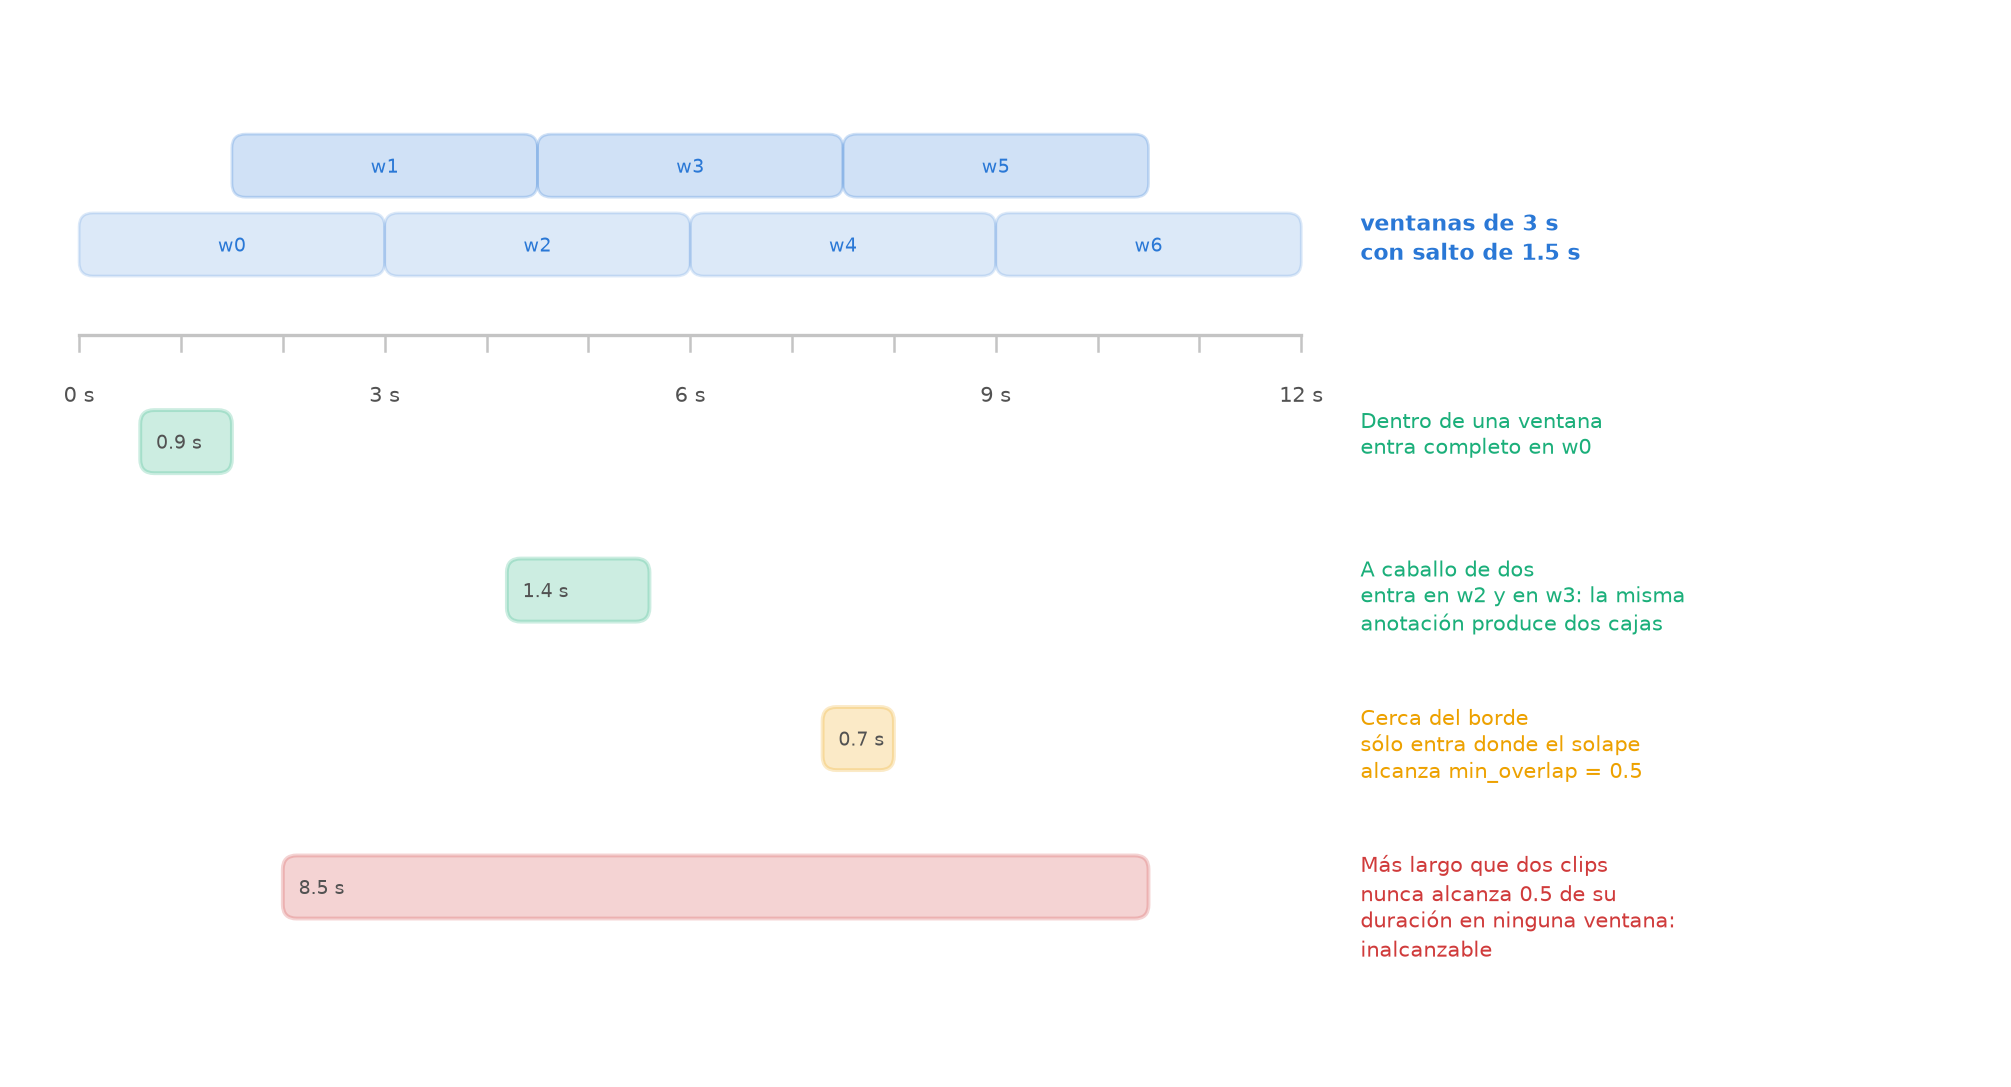
\includegraphics[width=\textwidth]{figures/windowing.png}
    \caption{Efecto del ventaneo.}
    \label{fig:windowing}
\end{figure}

\subsection{Densidad de eventos por ventana}

Conviene registrar cuántas anotaciones coinciden en una misma ventana de 3\,s: la
mediana es 1 y el máximo observado, 11; el 97\,\% de las ventanas con contenido
lleva cuatro cajas o menos. Es una propiedad del conjunto derivado, pero se
consigna aquí porque el Capítulo~\ref{cap:deteccion} la usa para dimensionar el
número de predicciones simultáneas que el decodificador debe sostener: el
presupuesto se fija sobre el máximo y no sobre la mediana.

A las ventanas con al menos una anotación se suma un 25\,\% de ventanas
\emph{vacías} tomadas al azar de tramos sin ninguna llamada. Sin ellas el modelo
nunca ve fondo puro —selva, lluvia, insectos— y aprende que en toda entrada hay
algo que reportar, que es exactamente el sesgo que la carga de revisión paga.


\subsection{Representación y normalización de las cajas}

Cada ventana se transforma en un espectrograma log-mel con los parámetros de la
Tabla~\ref{tab:preproc}. Log-mel es la representación con la que se materializa
el caché, y la que consumen las tres arquitecturas; la normalización de energía
por canal anunciada en la sección~\ref{sec:representacion} no la reemplaza sino
que se aplica encima, como capa entrenable de entrada de la arquitectura
propuesta (sección~\ref{sec:arquitectura}). La ablación que la compara contra la
compresión logarítmica fija está implementada en el repositorio, pero todavía no
medida. La columna de justificación registra qué falla con el
ajuste alternativo, que es la información que permite revisar un parámetro sin
repetir el experimento que lo fijó.

\begin{table}[htbp]
    \centering
    \caption[Parámetros de preprocesamiento]{Parámetros de preprocesamiento y motivo de cada elección}
    \label{tab:preproc}
    \small
    \begin{tabular}{@{}L{2.6cm}L{3.0cm}L{8.3cm}@{}}
        \toprule
        \textbf{Parámetro}       & \textbf{Valor}        & \textbf{Justificación} \\
        \midrule
        Ventana / salto          & 3,0\,s / 1,5\,s       &
        Contiene entera a 23 de las 25 clases; el costo es la fragmentación de
        las dos largas (Tabla~\ref{tab:ventaneo-largos})                          \\
        \addlinespace
        Solapamiento mínimo      & 0,5                   &
        Un evento entra en una ventana si la mitad de su parte visible cae
        dentro; medirlo contra la parte visible y no contra la duración total
        es lo que mantiene alcanzables a los eventos de más de 6\,s               \\
        \addlinespace
        Longitud de ventana STFT & 1\,024 (23\,ms)       &
        Más corta que los eventos más breves: 34\,ms el mínimo, 81\,ms la mediana
        de \texttt{sm/cc}                                                         \\
        \addlinespace
        Puntos de la FFT         & 4\,096                &
        Relleno con ceros: densifica la rejilla de frecuencia sin tocar la
        resolución temporal                                                       \\
        \addlinespace
        Salto STFT               & 400 (9\,ms)           &
        Produce 331 tramas por ventana                                            \\
        \addlinespace
        Bandas mel               & 128                   &
        Lo que espera el extractor preentrenado; 256 no dio ganancia medible      \\
        \addlinespace
        Rango de frecuencia      & 25\,Hz -- 22\,050\,Hz &
        Un techo de 16\,kHz truncaba la mitad de las cajas de \texttt{sb/spc},
        cuya frecuencia superior media es 16\,110\,Hz                             \\
        \bottomrule
    \end{tabular}
\end{table}

Las cajas se normalizan al formato de centro, ancho y alto en el intervalo
$[0,1]$, con el eje de frecuencia mapeado a través de la misma escala mel que
produce la imagen. La consecuencia es que una caja significa lo mismo en el
espacio de píxeles que sobre la pantalla del analista: el rectángulo que el
modelo predice es directamente el rectángulo que Raven dibuja, sin
reinterpretación. La Figura~\ref{fig:window-example} muestra una ventana de
entrenamiento tal como el modelo la recibe.

\begin{figure}[htbp]
    \centering
    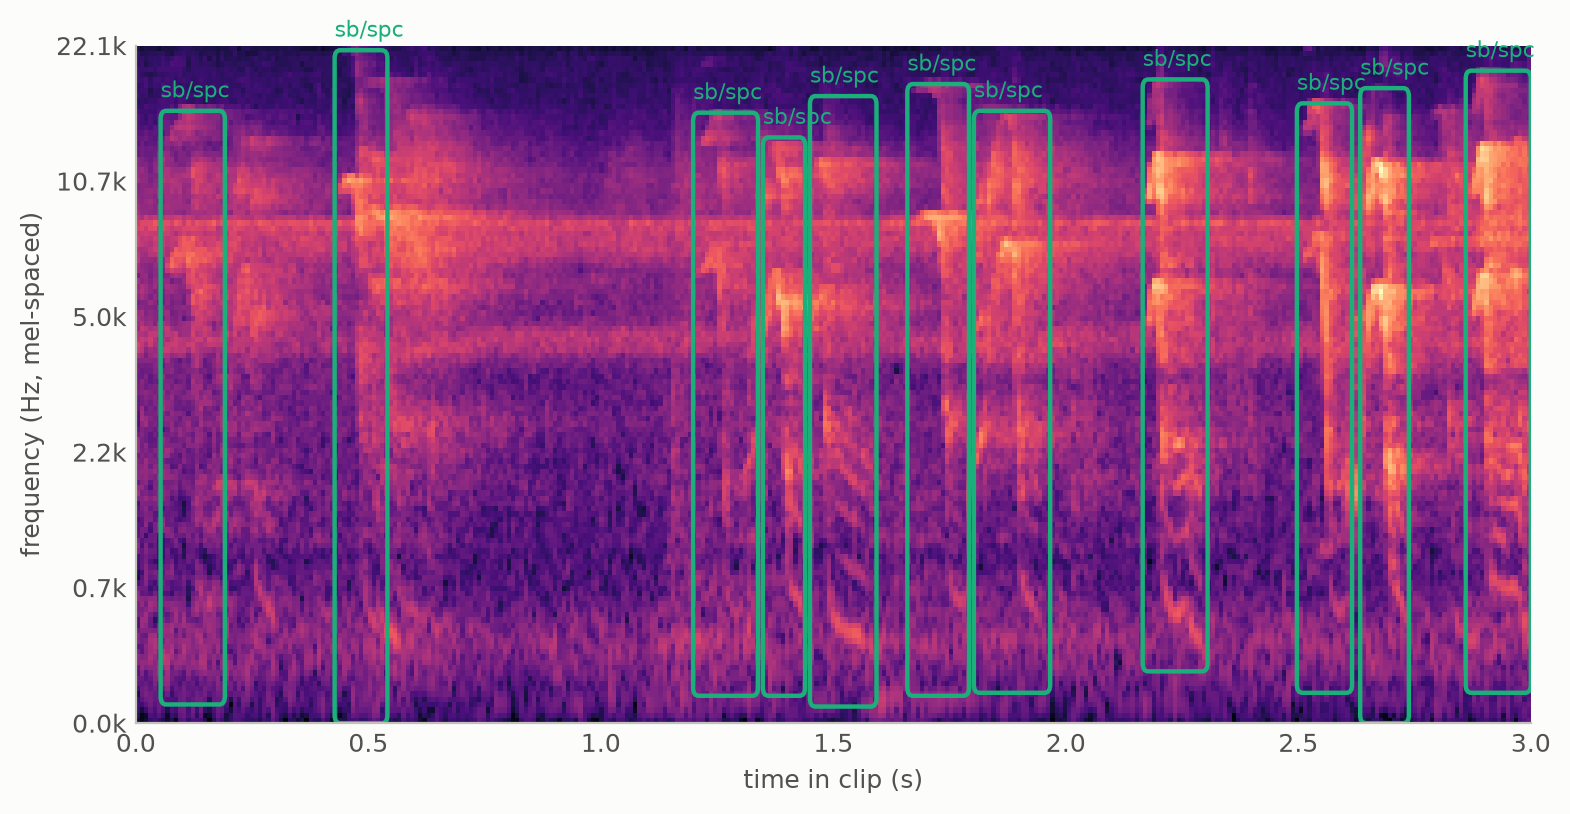
\includegraphics[width=\textwidth]{figures/window_example.png}
    \caption[Ventana de entrenamiento]{Una ventana de entrenamiento: espectrograma log-mel de 3\,s con los
        parámetros de la Tabla~\ref{tab:preproc} y las cajas objetivo superpuestas
        en el marco normalizado. Las once cajas \texttt{sb/spc} de este clip son el
        caso más denso observado en todo el conjunto.}
    \label{fig:window-example}
\end{figure}

\begin{figure}[htbp]
    \centering
    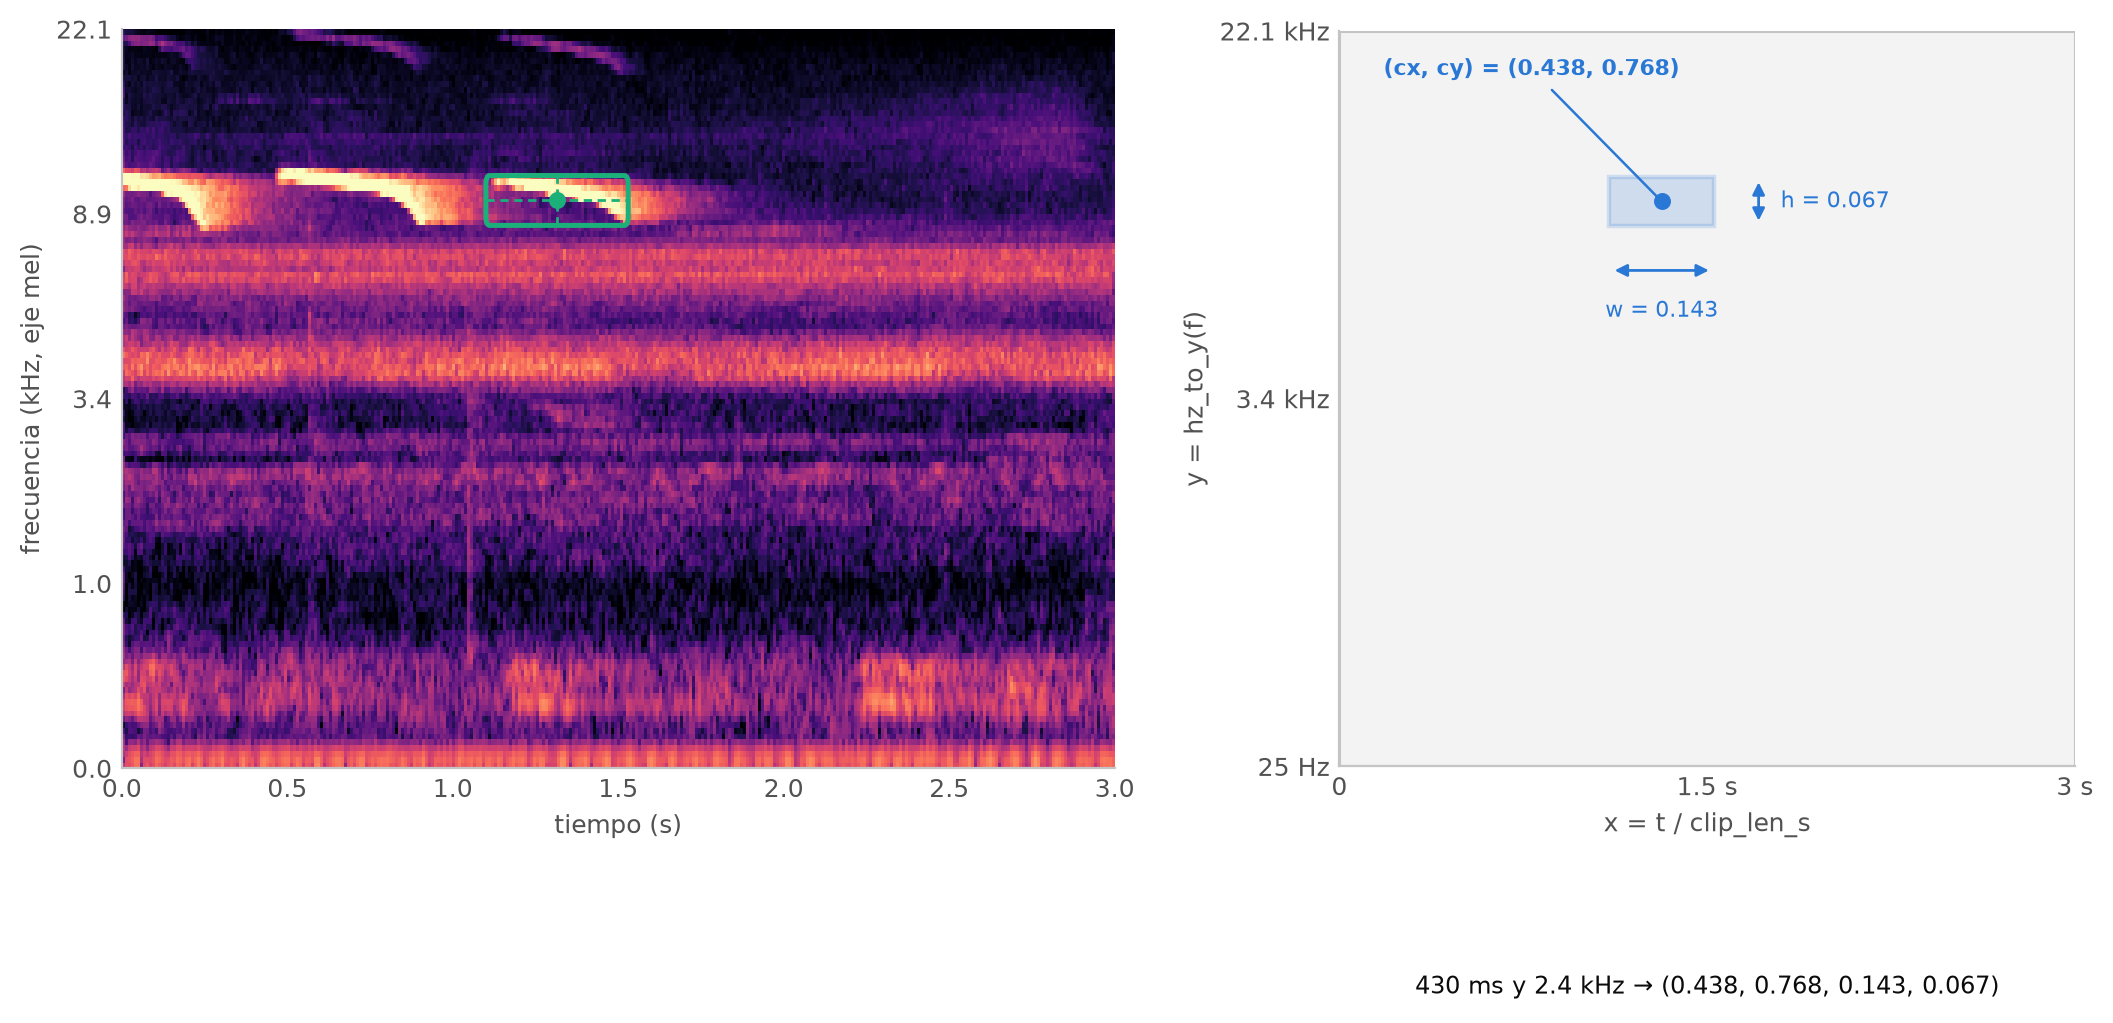
\includegraphics[width=\textwidth]{figures/box_coordinates.png}
    \caption{Coordenadas de la caja.}
    \label{fig:box-coordinates}
\end{figure}

\section{Balance del conjunto de experimento}
\label{sec:revision}

Las 25 clases seleccionadas cubren el 92,5\,\% del material curado, pero la
selección no corrige las dos causas estructurales que este capítulo documentó, y
conviene dejar dicho qué queda en pie antes de leer los resultados del
Capítulo~\ref{cap:deteccion}.

\rotulo{El desbalance no desaparece: se traslada.} Entre \texttt{ac/bc}, la clase
mayoritaria una vez descontada la fragmentación de \texttt{as/hc}, con 2\,886
cajas de entrenamiento, y \texttt{sb/sc}, con 126, median más de veinte veces, y el orden de magnitud se mantiene aunque el umbral baje o suba
(Figura~\ref{fig:boxes-split}). La partición sí preserva el balance: cada clase
conserva aproximadamente la misma proporción en las tres particiones, que es lo
que permite comparar el desempeño por clase entre validación y prueba sin
atribuir a la arquitectura una diferencia de composición.

\begin{figure}[htbp]
    \centering
    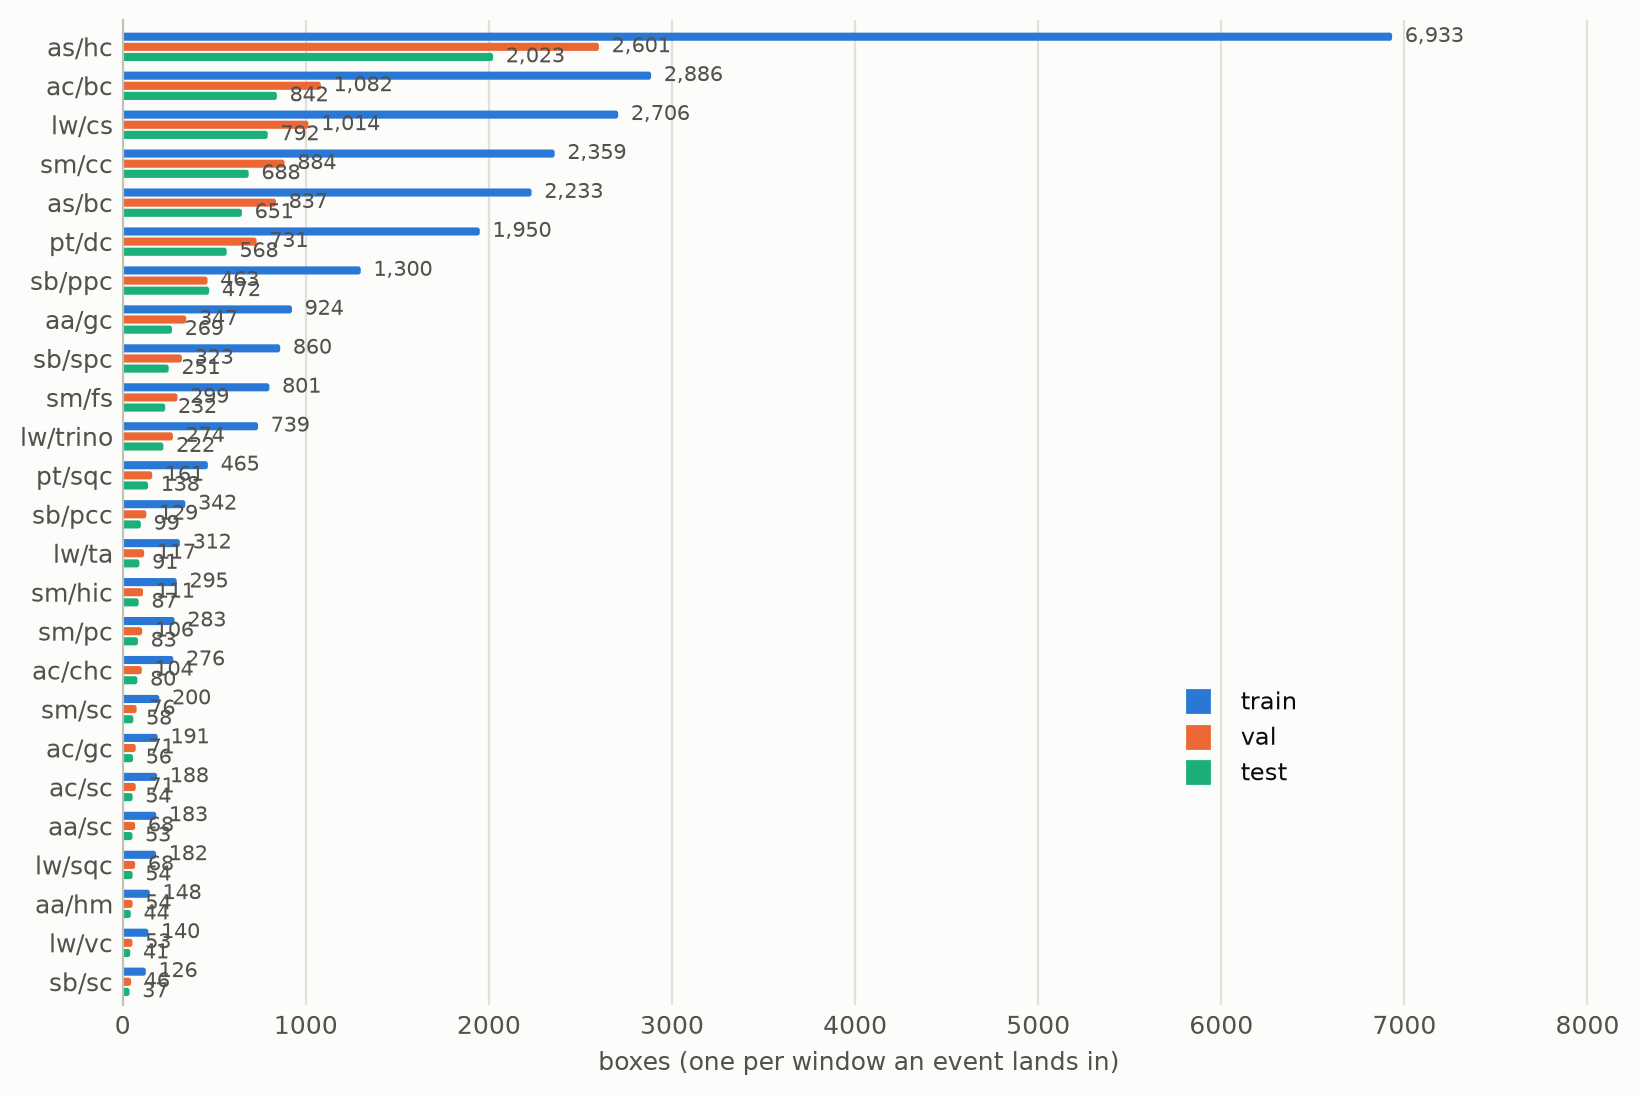
\includegraphics[width=\textwidth]{figures/boxes_per_split.png}
    \caption[Cajas por clase y partición]{Cajas por clase y partición. El balance se preserva entre
        particiones; el desbalance entre clases se mantiene, con más de un orden de
        magnitud entre la clase mayoritaria y las que apenas superan el umbral.}
    \label{fig:boxes-split}
\end{figure}

\rotulo{La escasez y la arquitectura se confunden en el análisis por clase.}
Once de las veinticinco clases aportan menos de 300 cajas de entrenamiento.
Cuando una de ellas obtiene mal \textit{recall}, la causa puede ser el modelo o
puede ser que nunca vio material suficiente, y el Capítulo~\ref{cap:deteccion}
solo puede separar ambas cosas comparando el comportamiento de las cuatro
arquitecturas sobre la misma clase: una clase que todas fallan por igual es
escasez; una que unas recuperan y otras no es arquitectura.

\rotulo{La densidad por ventana es baja.} La mediana de cajas por ventana de
3\,s es 1 y el máximo 11 (Figura~\ref{fig:boxes-window}). El presupuesto de
predicciones simultáneas del decodificador se dimensiona sobre el máximo, no
sobre la mediana, y las 64 consultas de la arquitectura propuesta lo cubren con
holgura.

\begin{figure}[htbp]
    \centering
    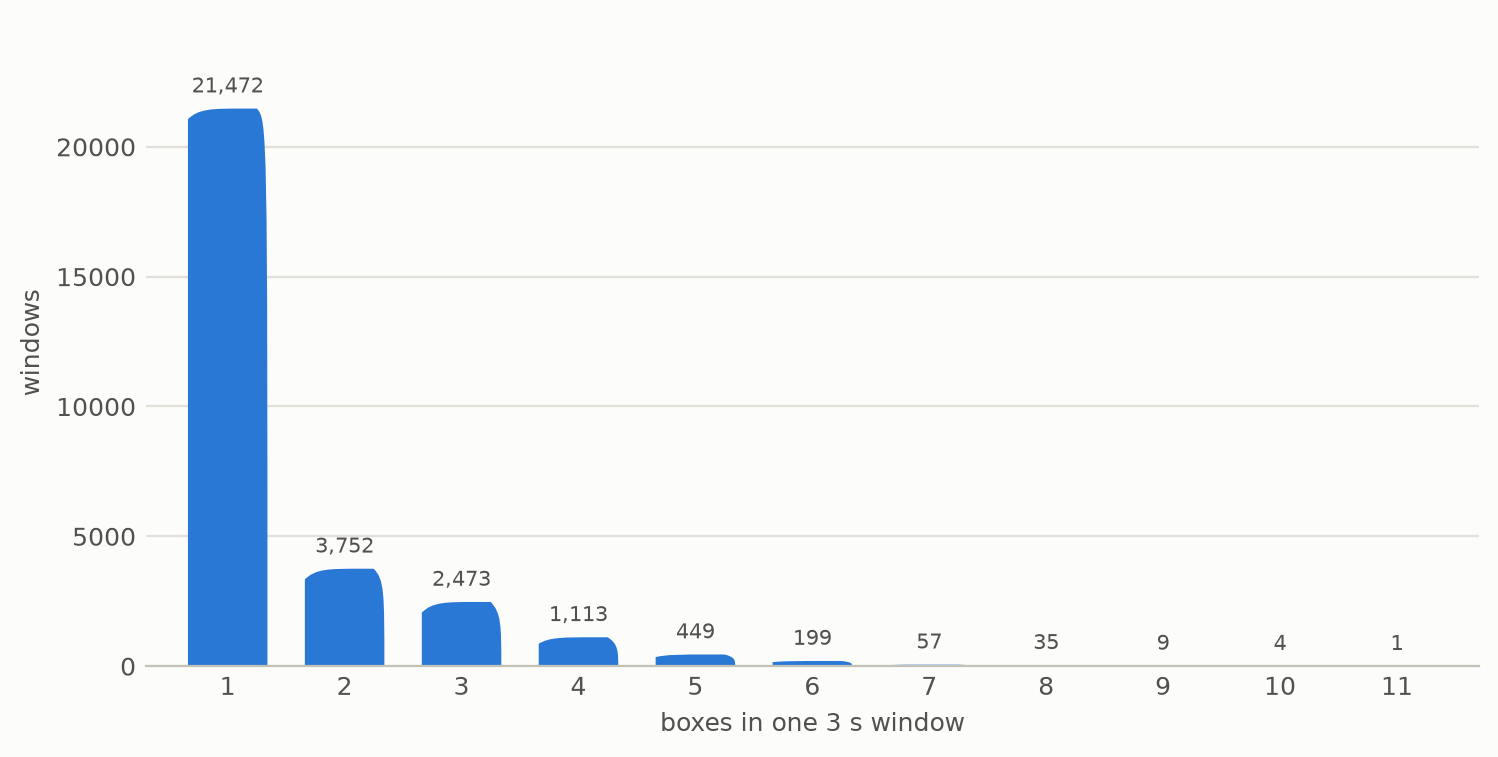
\includegraphics[width=0.92\textwidth]{figures/boxes_per_window.png}
    \caption[Cajas anotadas por ventana]{Cajas anotadas por ventana de 3\,s: mediana 1, máximo 11.}
    \label{fig:boxes-window}
\end{figure}


\section{Ficha del conjunto derivado (RE1.3)}

La documentación del conjunto sigue la estructura de las \textit{datasheets} para
conjuntos de datos, que proponen registrar motivación, composición, proceso de
recolección, transformaciones aplicadas y usos recomendados, con el propósito de
aumentar la transparencia y la rendición de cuentas \citep{gebru_2021}. La ficha
distingue de forma explícita dos capas de responsabilidad.

\rotulo{Conjunto primario.} Las grabaciones y las anotaciones originales,
producidas por el equipo de investigación. La ficha documenta su origen, el
equipo de captura, la frecuencia de muestreo y el procedimiento de anotación en
Raven, pero no reclama su autoría.

\rotulo{Conjunto derivado.} El resultado de aplicar el protocolo de la
sección~\ref{sec:protocolo}: normalización de etiquetas, vocabulario cerrado,
saneamiento geométrico, selección del subconjunto, partición por archivo de
grabación y ventaneo. Esta capa sí es contribución de esta tesis, y la ficha
registra cada transformación junto con lo que descarta.

La ficha declara además, como limitaciones conocidas del conjunto derivado:

\begin{itemize}[nosep]
    \item La fragmentación de las llamadas largas bajo el ventaneo de 3\,s
          (Tabla~\ref{tab:ventaneo-largos}): \texttt{as/hc} y \texttt{pt/dc} sobreviven
          como series de cajas recortadas al borde de la ventana, y el conjunto no
          incluye ningún mecanismo que las reagrupe en el evento original.
    \item Las tres clases de frase excluidas por anidamiento
          (sección~\ref{sec:silabas}), que dejan sin cubrir el nivel superior de la
          jerarquía vocal.
    \item Los once tipos de llamada en vocabulario que no alcanzan el umbral de
          100 anotaciones (466 registros) y quedan fuera del experimento, entre ellos la
          única clase de CC, que hace que el conjunto de experimento cubra siete
          especies y no ocho.
    \item Los 16 pares fuera de vocabulario (328 registros) pendientes de
          revisión por el equipo de investigación.
    \item Las once clases con menos de 300 cajas de entrenamiento, cuyo
          desempeño individual no puede atribuirse limpiamente a la arquitectura.
    \item La heterogeneidad geométrica de \texttt{ac/bc}, \texttt{sm/fs} y
          \texttt{sb/ppc} (Figura~\ref{fig:facets}), que sugiere etiquetas que agrupan
          variantes distintas de llamada.
    \item La ausencia de una medición de acuerdo entre anotadores, que impide
          separar el error del modelo del techo impuesto por la propia tarea.
\end{itemize}

% TODO Decidir con el equipo si el conjunto se libera y en qué términos.
% Si hay restricciones por ubicación de especies amenazadas, decláralas
% aquí como limitación legítima, no las omitas.


% ===================================================================
% CAPÍTULO 5
% ===================================================================
\chapter{Detección, Evaluación y Utilidad Operativa (OE2 y OE3)}
\label{cap:deteccion}

\section{Arquitectura propuesta y línea base (RE2.1)}
\label{sec:arquitectura}
% TODO Redactar.
% NOTA: el informe E3 documenta un prototipo previo basado en YOLOv2 con
% anchor boxes calculadas por K-Means sobre (duration_s, bandwidth_hz),
% k=5 por par (especie, tipo de llamada), y un tensor objetivo
% S x S x k x (5+C). Ese material NO se trasladó al cuerpo porque
% contradice la arquitectura sin anclas que plantea este capítulo.
% Decide antes de redactar: o se recupera como línea base explícita
% (y entonces la figura figures/image14.png entra aquí), o se menciona
% solo en el capítulo 6 como iteración descartada.
% TODO TABLA 5.1: desviaciones respecto de la receta estándar, con la
%                  falla que cada una corrige. Las cuatro figuras de
%                  abajo la ilustran; la tabla sigue haciendo falta.
% ===================================================================
\begin{figure}[htbp]
    \centering
    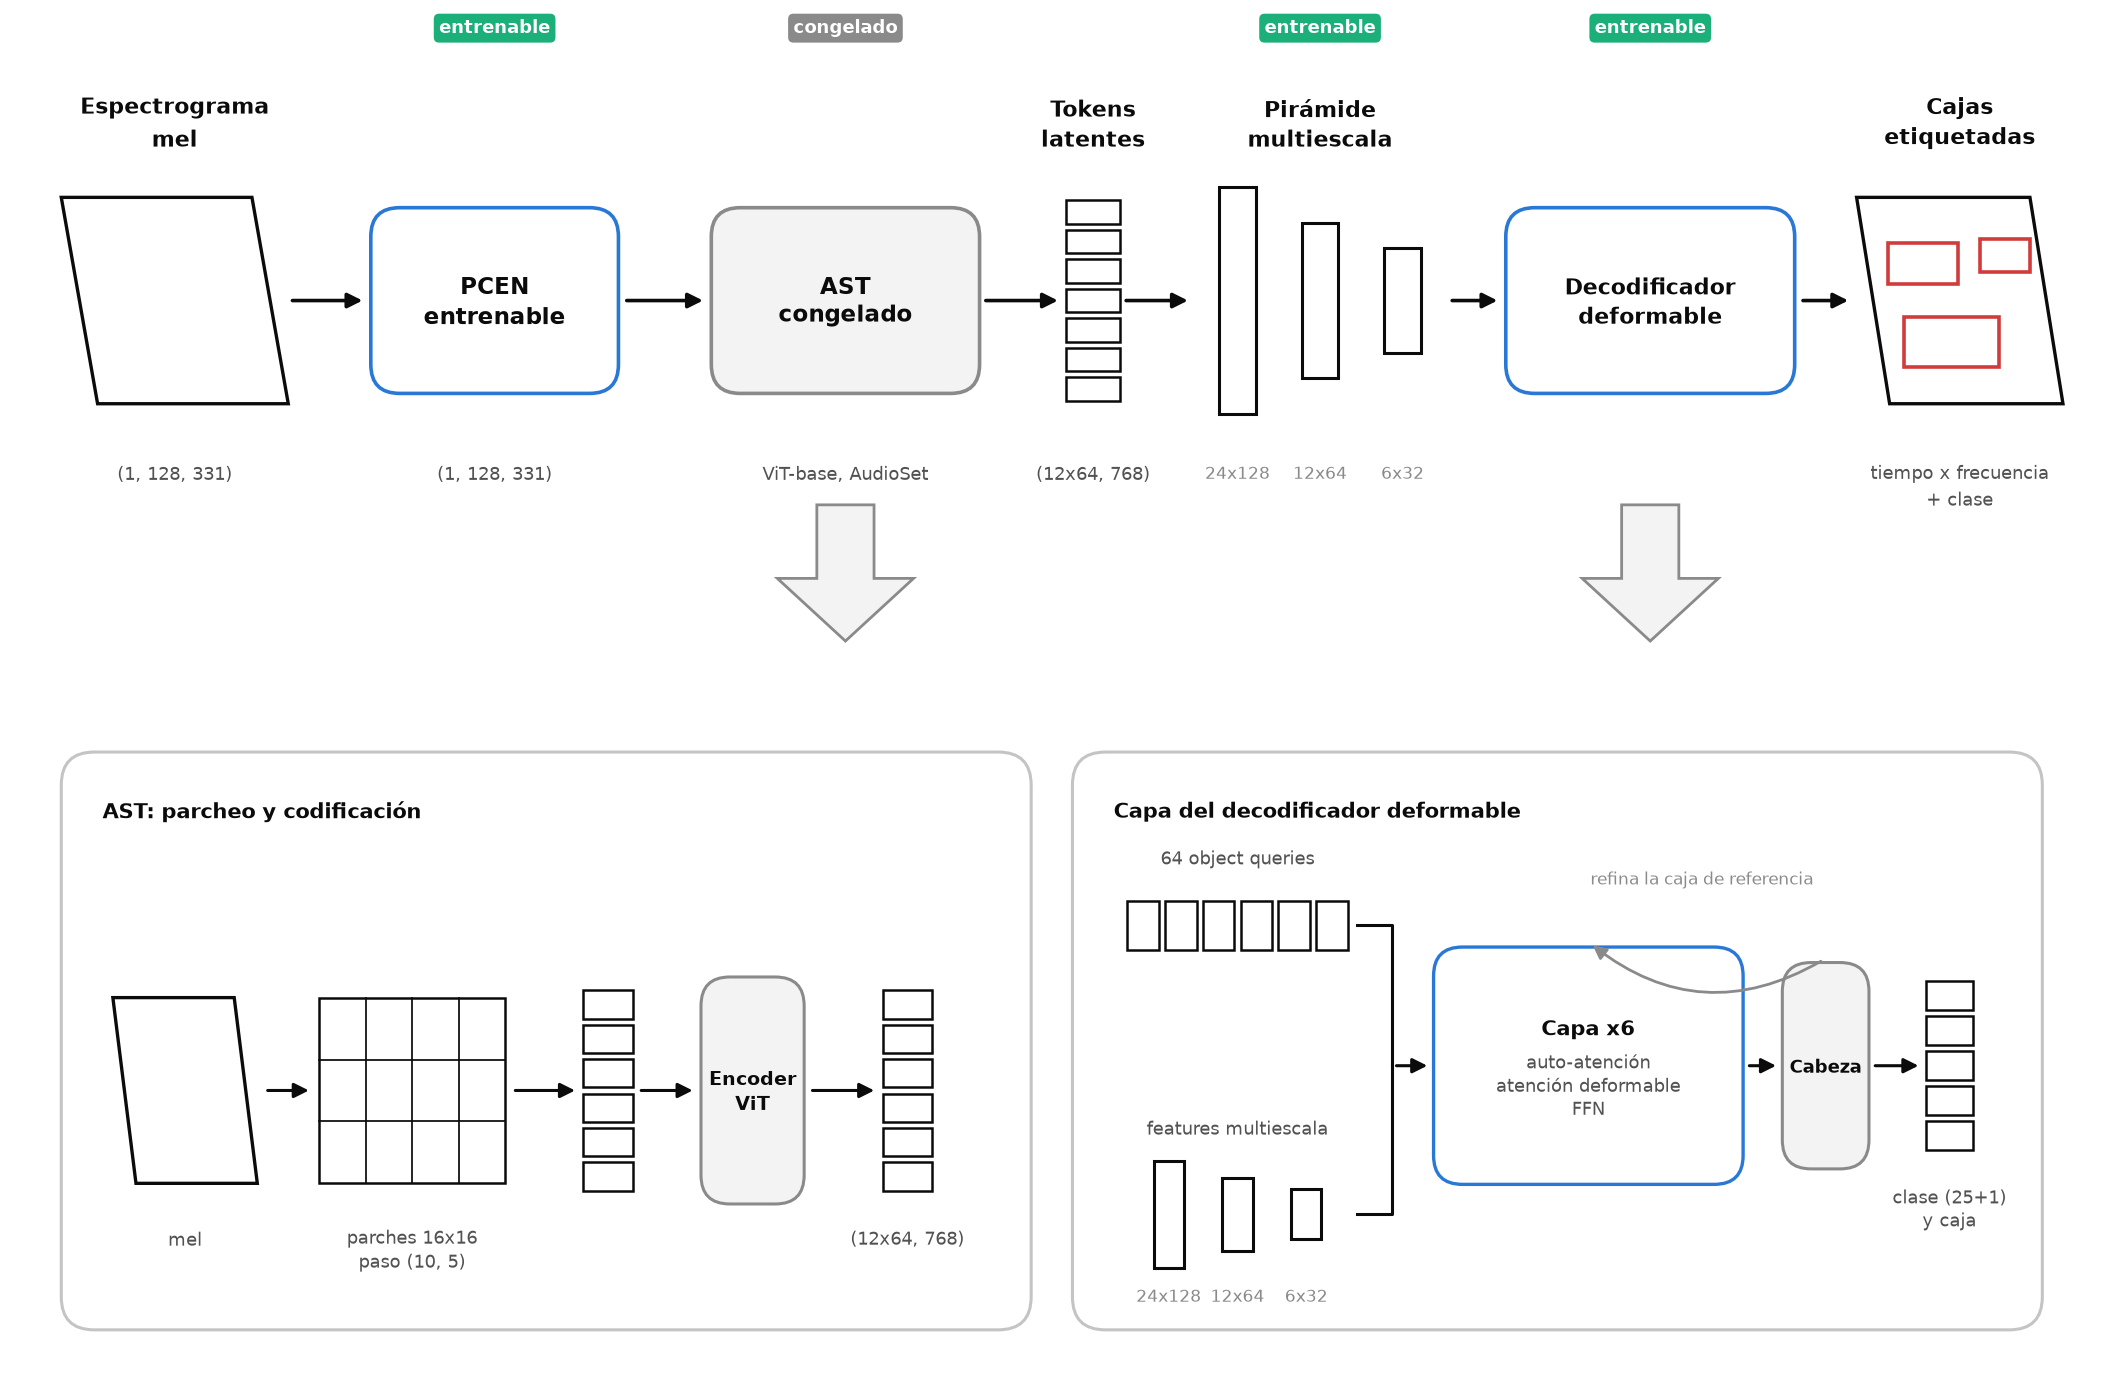
\includegraphics[width=\textwidth]{figures/architecture.png}
    \caption{Arquitectura propuesta.}
    \label{fig:architecture}
\end{figure}

\begin{figure}[htbp]
    \centering
    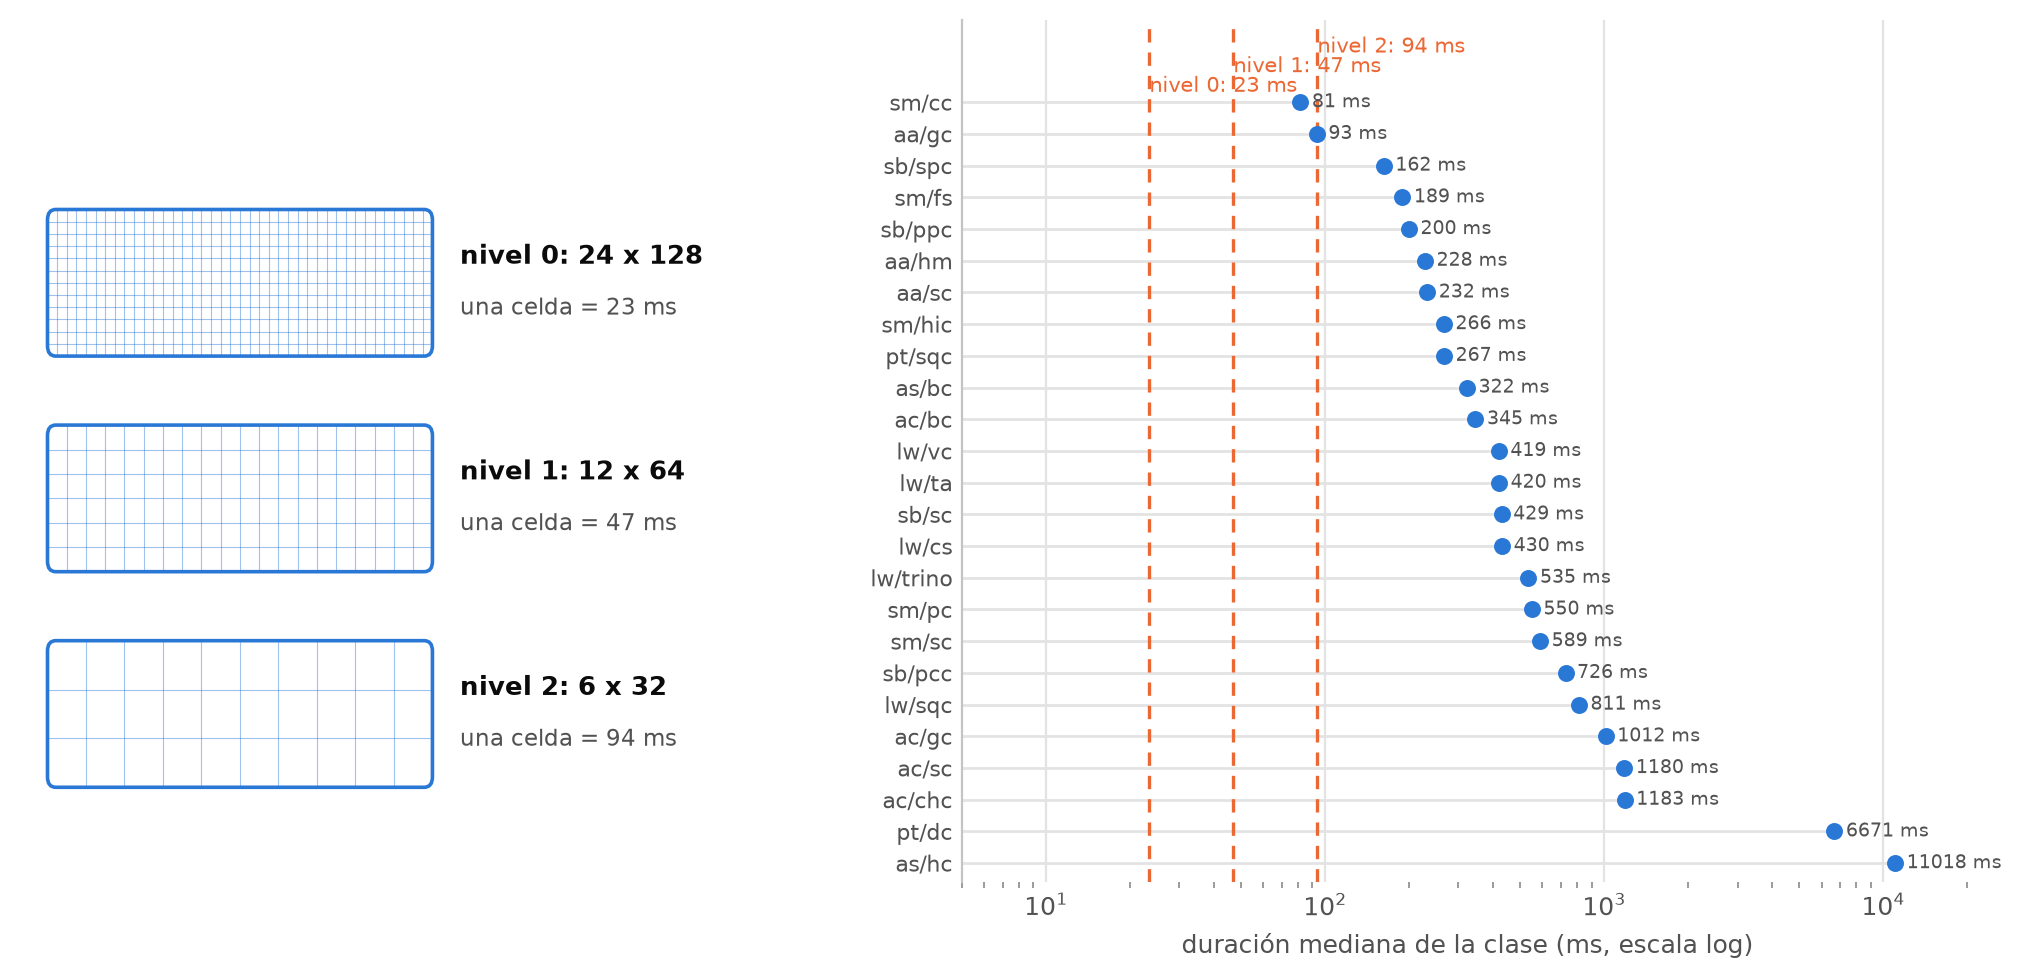
\includegraphics[width=\textwidth]{figures/multiscale_pyramid.png}
    \caption{Pirámide multiescala.}
    \label{fig:multiscale-pyramid}
\end{figure}

\begin{figure}[htbp]
    \centering
    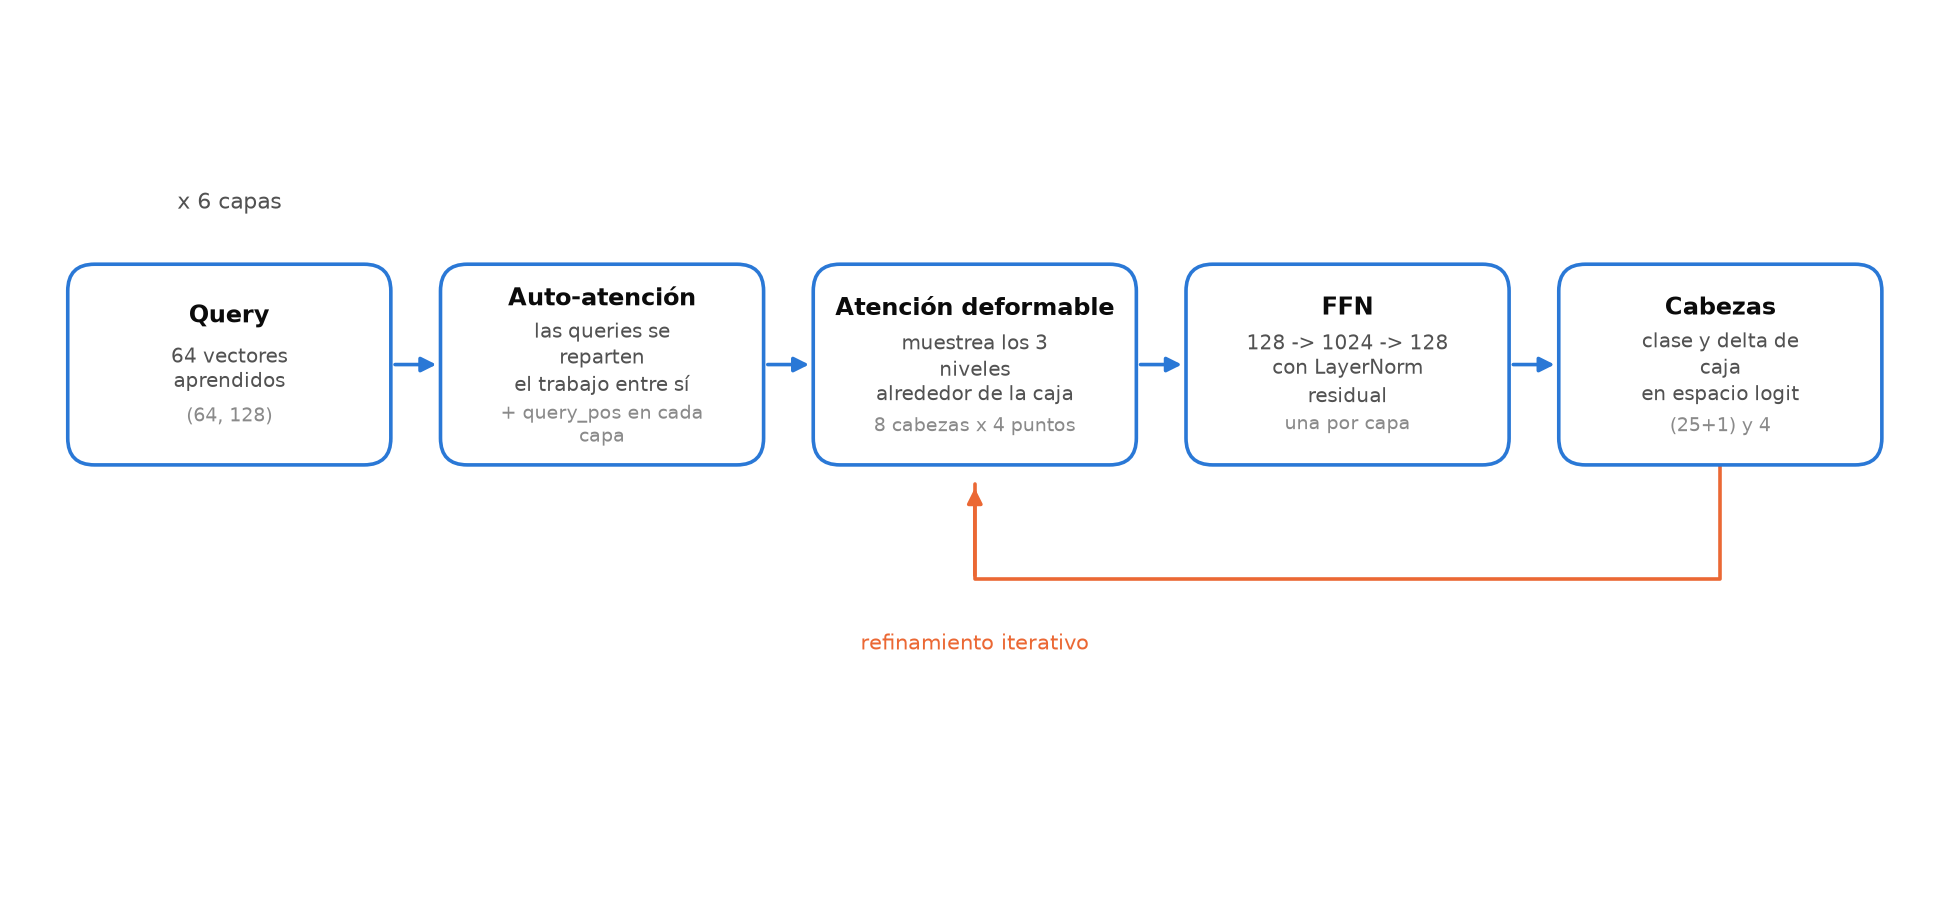
\includegraphics[width=\textwidth]{figures/decoder_layer.png}
    \caption{Capa del decodificador.}
    \label{fig:decoder-layer}
\end{figure}

\begin{figure}[htbp]
    \centering
    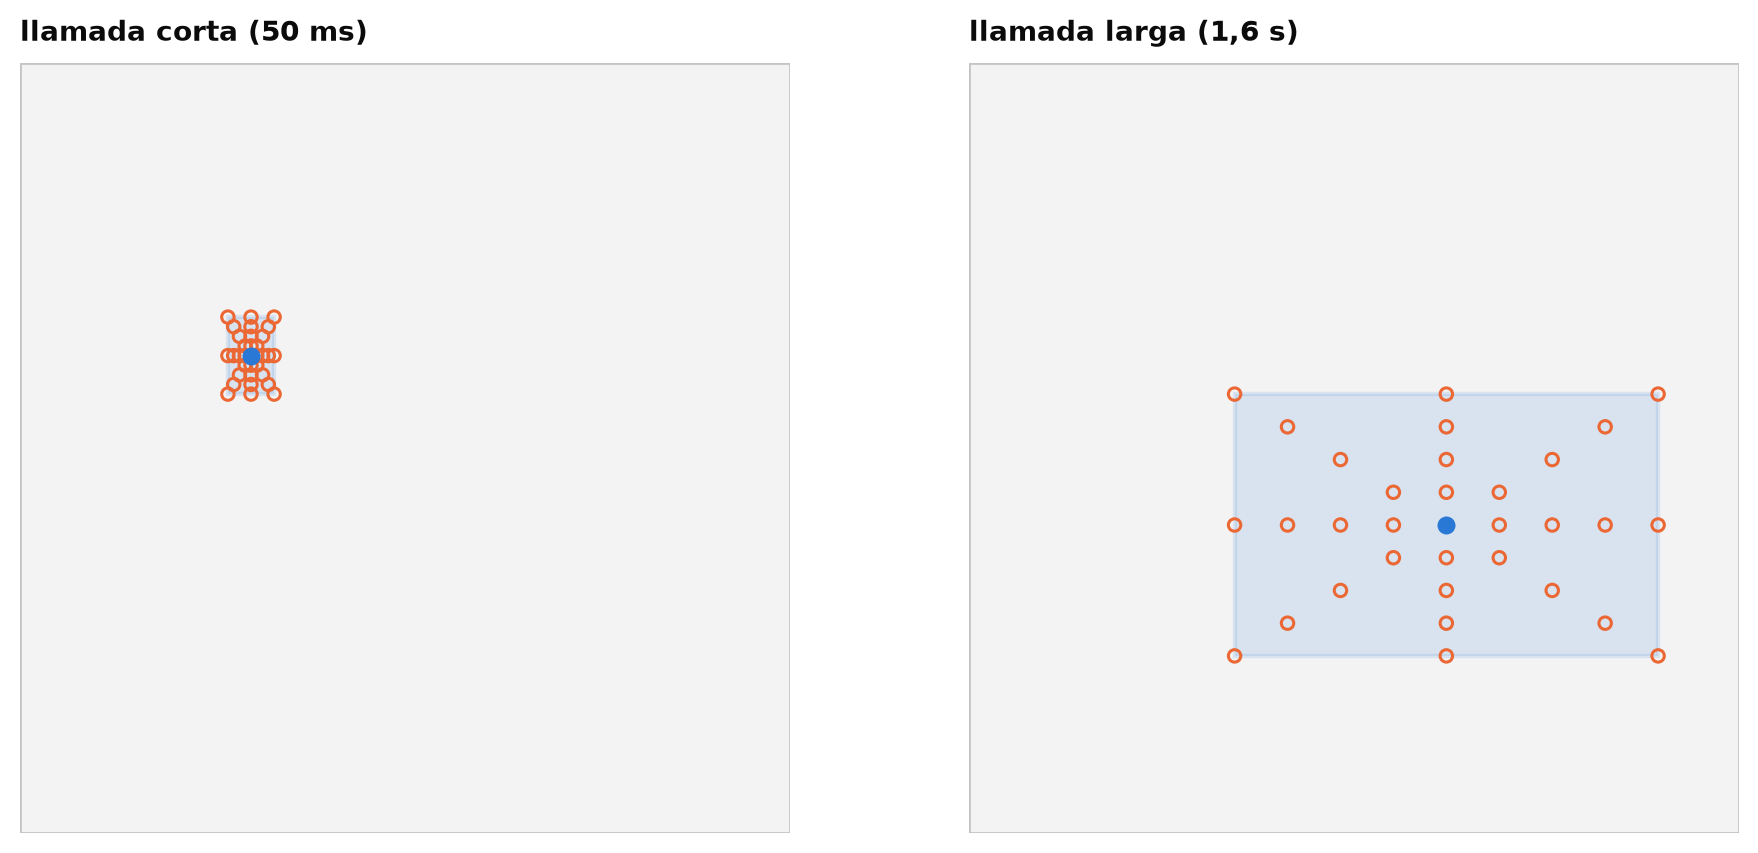
\includegraphics[width=\textwidth]{figures/deformable_sampling.png}
    \caption{Muestreo deformable.}
    \label{fig:deformable-sampling}
\end{figure}

\section{Pipeline de entrenamiento e inferencia (RE2.2)}
% TODO Redactar: parámetros de preprocesamiento, función de pérdida,
% emparejamiento, selección de checkpoint.
% TODO TABLA 5.2: parámetros de preprocesamiento con su justificación.

\begin{figure}[htbp]
    \centering
    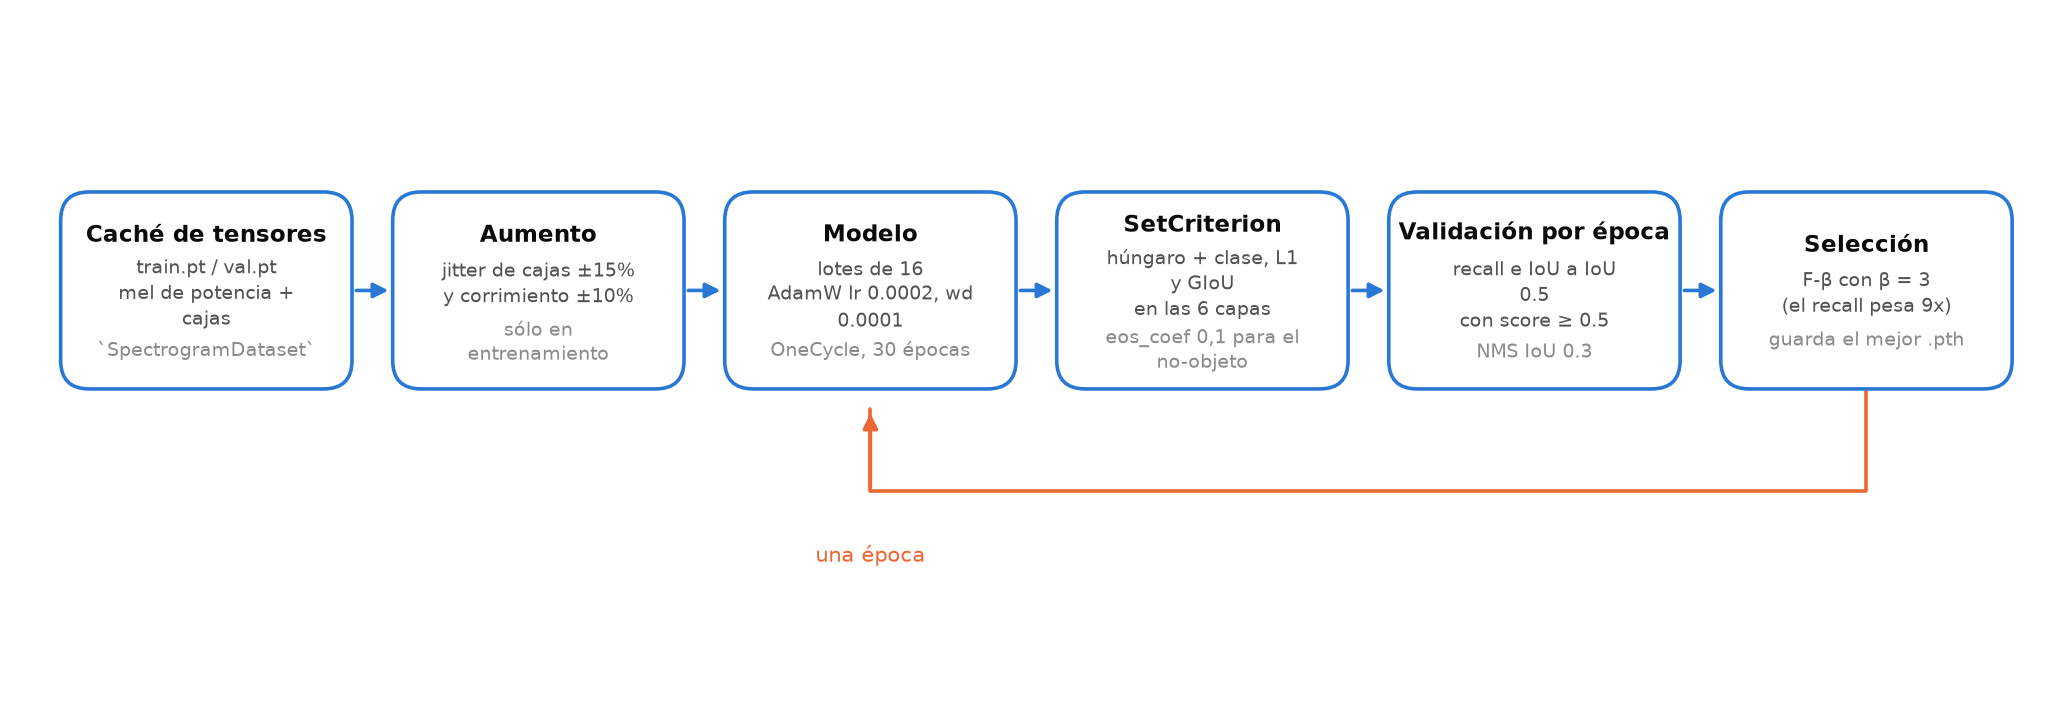
\includegraphics[width=\textwidth]{figures/training_pipeline.png}
    \caption{Pipeline de entrenamiento.}
    \label{fig:training-pipeline}
\end{figure}

\begin{figure}[htbp]
    \centering
    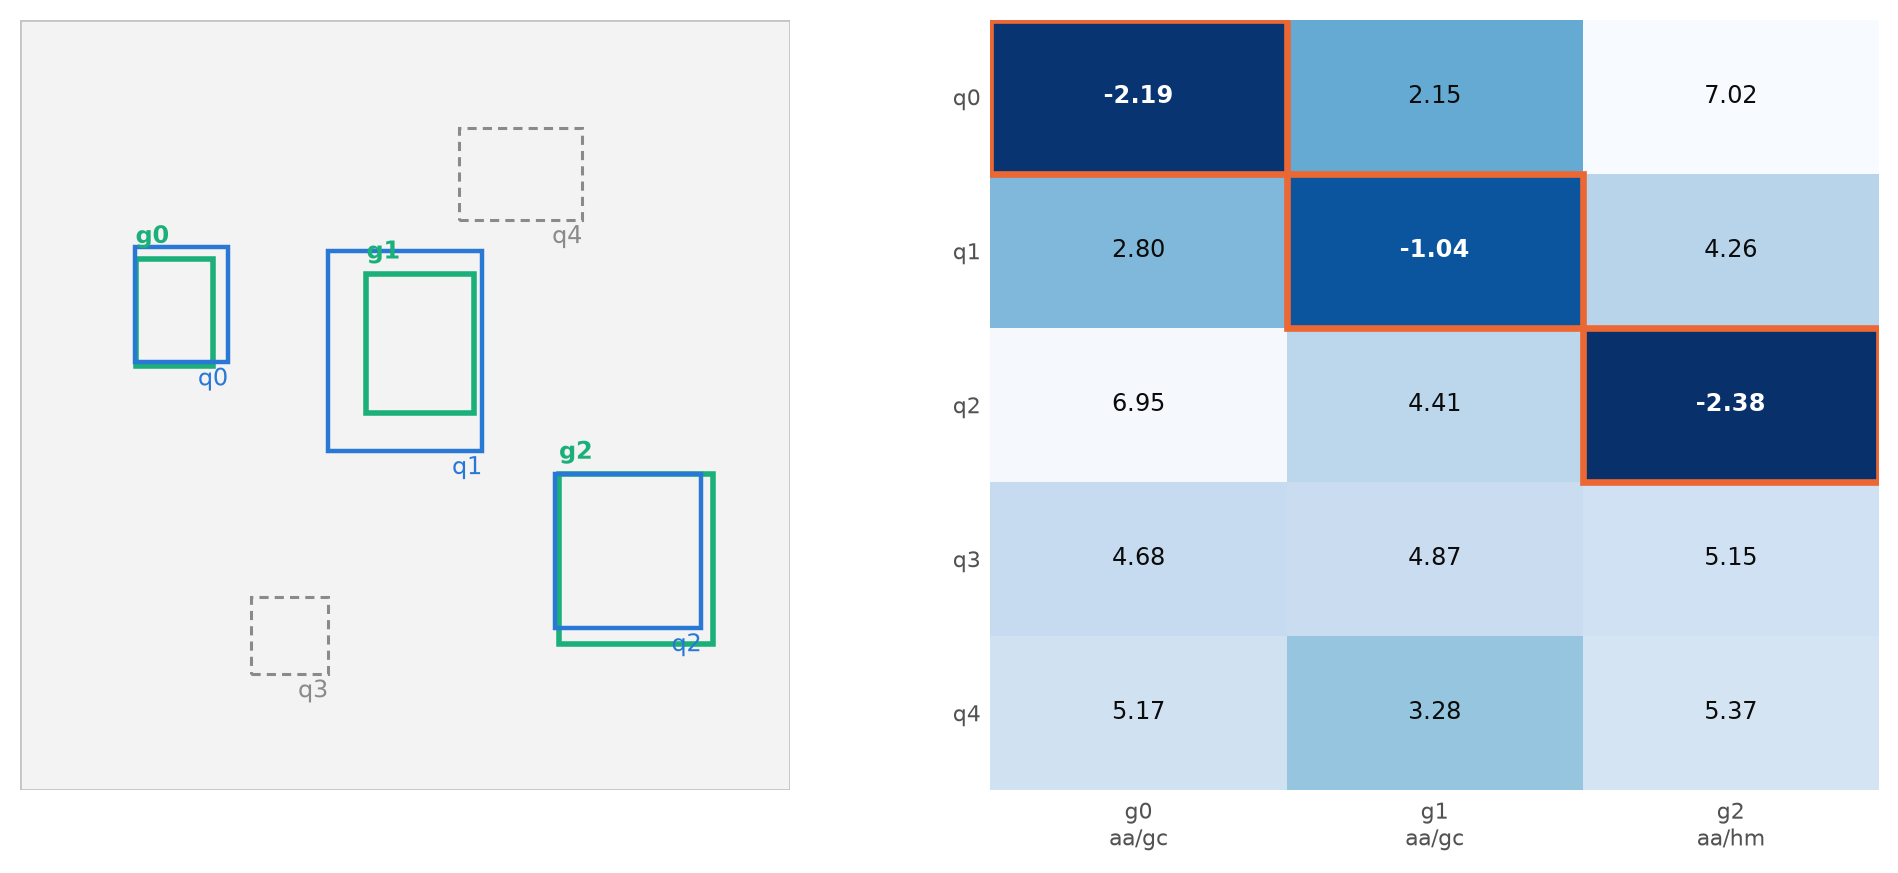
\includegraphics[width=\textwidth]{figures/hungarian_matching.png}
    \caption{Emparejamiento húngaro.}
    \label{fig:hungarian-matching}
\end{figure}

% FIGURA PENDIENTE: figures/training_curves.png
% Falta el metrics.jsonl de la corrida: `train.py` lo escribe en
% logs/<fecha>/ de la máquina donde se entrena. Copiá esa carpeta a
% logs/ y volvé a correr la sección 7.7 del cuaderno.
% ===================================================================

\begin{figure}[htbp]
    \centering
    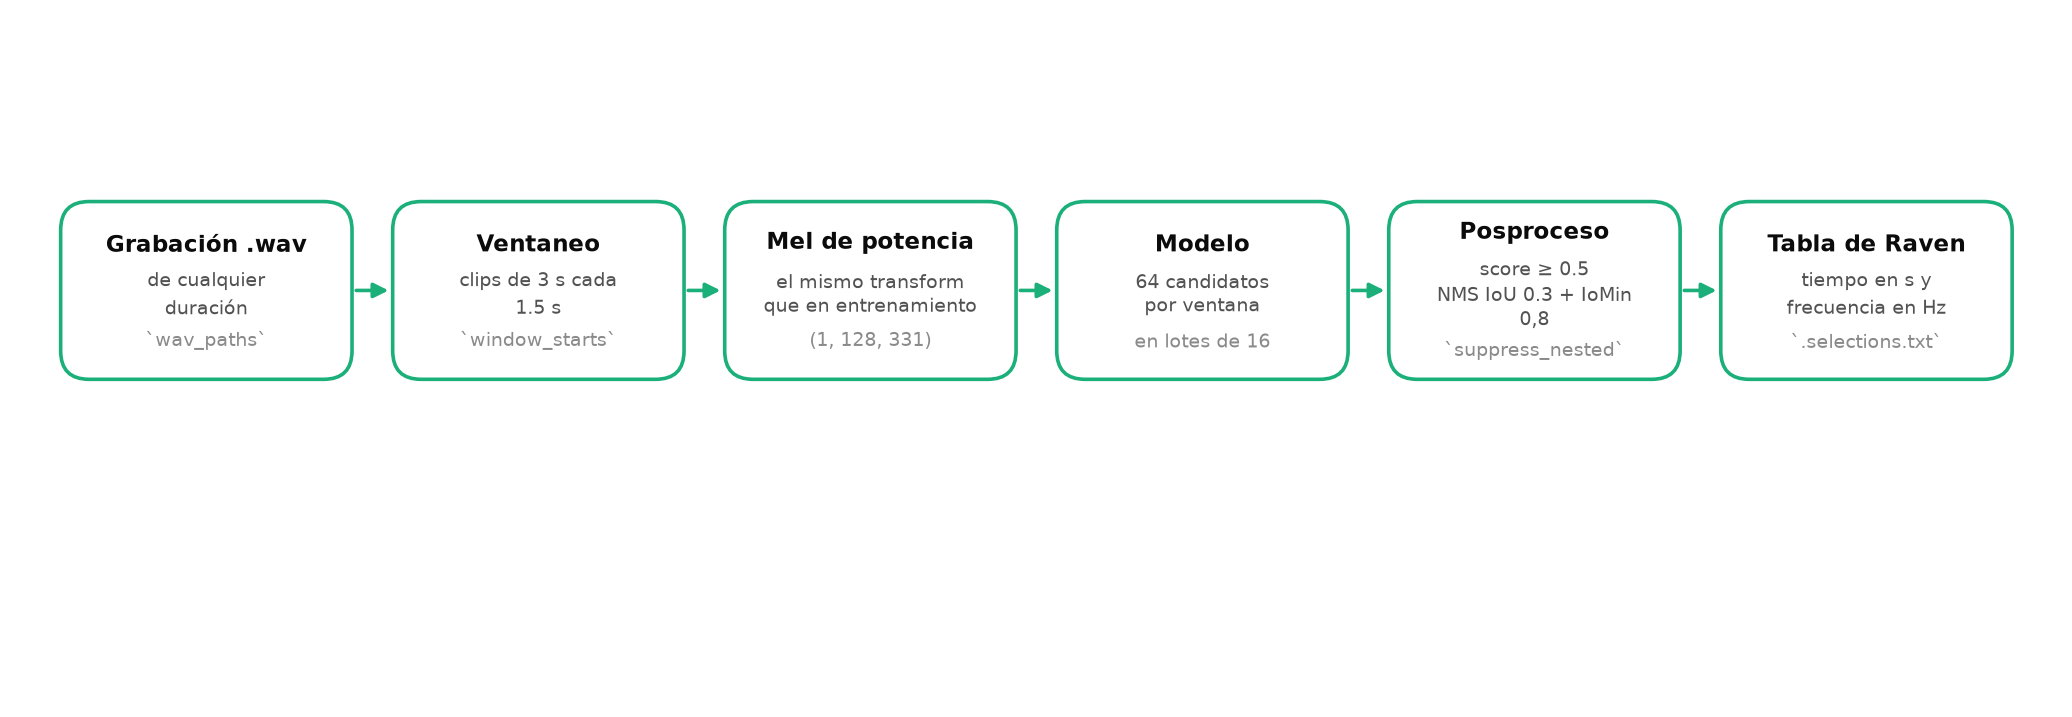
\includegraphics[width=\textwidth]{figures/inference_pipeline.png}
    \caption{Pipeline de inferencia.}
    \label{fig:inference-pipeline}
\end{figure}

\section{Protocolo de evaluación}
% TODO Redactar: los tres ejes (detección, encuadre, clasificación) y
% por qué se puntúan por separado.
% TODO TABLA 5.3: eje / pregunta que responde / métrica.

\begin{figure}[htbp]
    \centering
    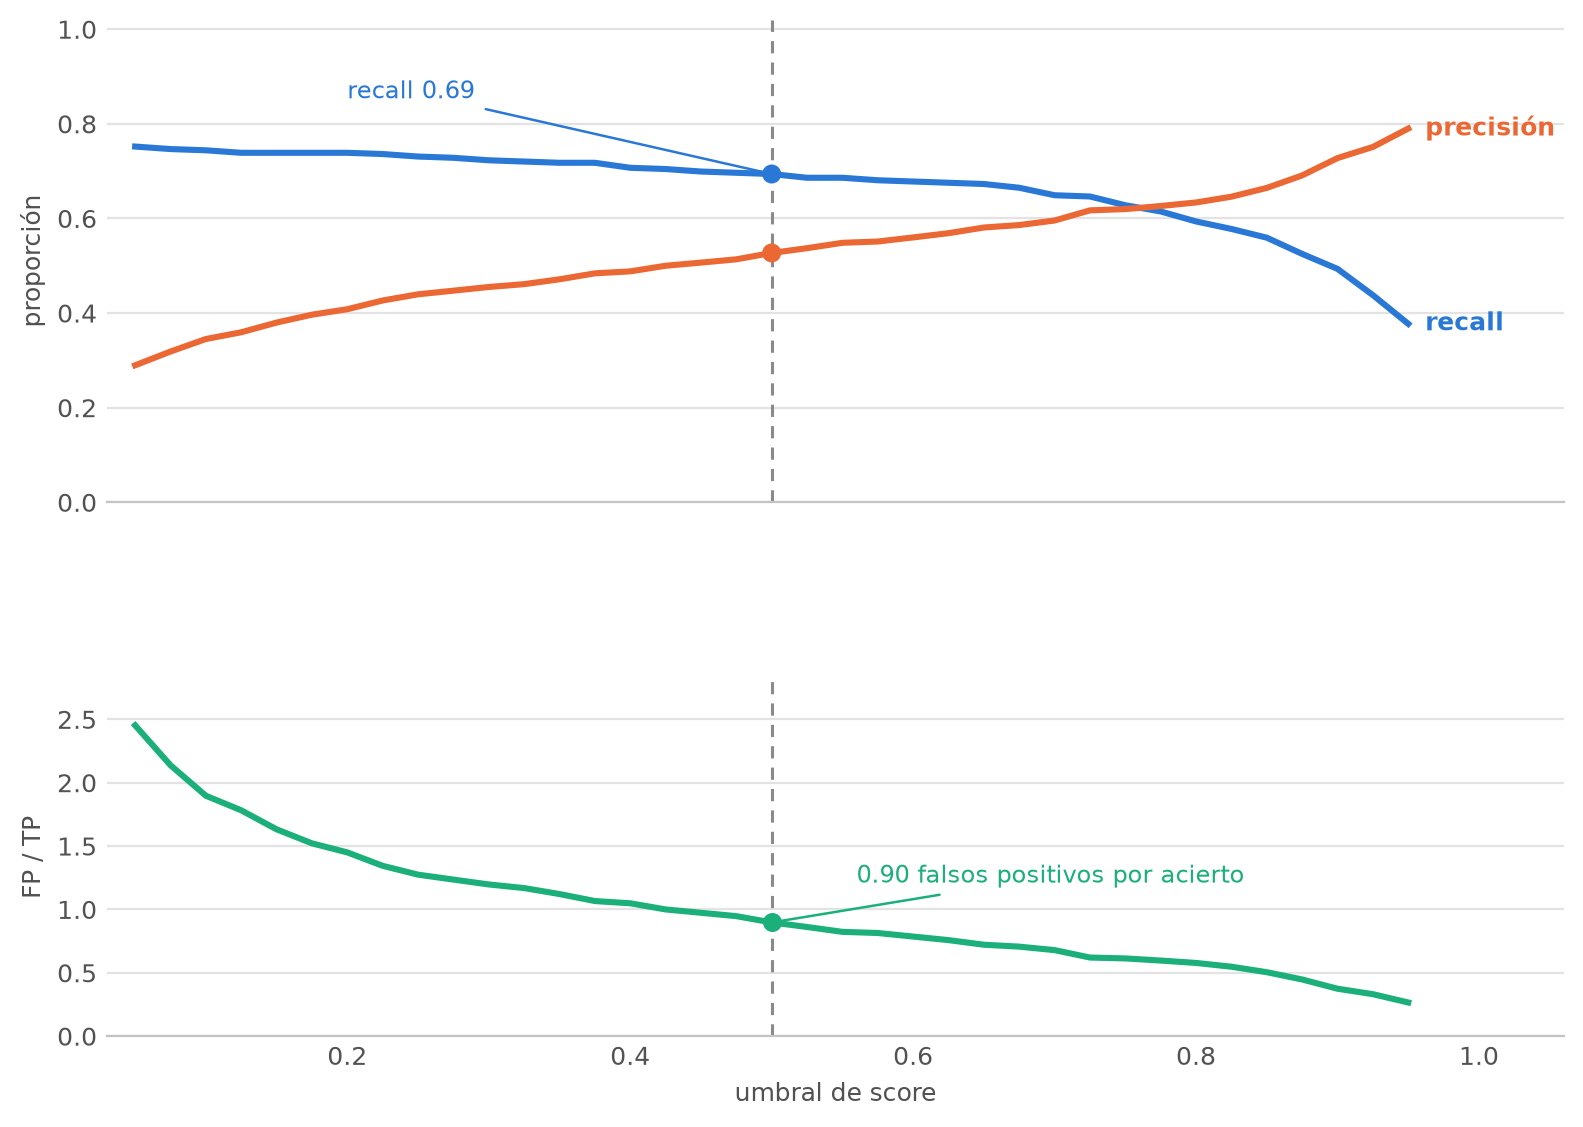
\includegraphics[width=0.9\textwidth]{figures/score_sweep.png}
    \caption{Umbral de confianza.}
    \label{fig:score-sweep}
\end{figure}

\section{Resultados (RE2.3)}
\label{sec:resultados-deteccion}

Esta sección compara cuatro configuraciones entrenadas sobre el mismo conjunto
derivado de 25 clases, con la misma partición y el mismo protocolo de evaluación.
Las cifras de validación sirvieron para elegir el \textit{checkpoint}; las de
prueba se reportan una sola vez, sobre el modelo ya elegido.

% TODO TABLA: estudio de ablación acumulativo (PCEN vs. log-mel, niveles de la
% pirámide, backbone congelado vs. fine-tune). La rama de control existe en el
% repositorio pero ninguna corrida la midió todavía.
% TODO FIGURA 5.3: ejemplos cualitativos de detección, incluyendo AL MENOS UN
% CASO DIFÍCIL (escena densa con especies solapadas). Mostrar solo los aciertos
% debilita el capítulo ante el jurado.

\subsection{Configuraciones comparadas}

La Tabla~\ref{tab:configuraciones} resume qué se compara. Las cuatro
configuraciones comparten datos y protocolo, pero no presupuesto de
entrenamiento, y esa asimetría condiciona toda lectura posterior: la arquitectura
propuesta ajusta 3,1 millones de parámetros sobre un extractor congelado,
mientras que las dos líneas base ajustan todos los suyos partiendo de pesos de
COCO.

\begin{table}[htbp]
    \centering
    \small
    \begin{threeparttable}
        \caption[Configuraciones comparadas]{Configuraciones comparadas sobre el conjunto de 25 clases}
        \label{tab:configuraciones}
        \begin{tabular}{@{}L{3.5cm}L{3.4cm}rrL{3.4cm}@{}}
            \toprule
            \textbf{Configuración}                & \textbf{Extractor}          & \thead{Parám.\\totales} & \thead{Parám.\\entren.} & \textbf{Selección del \textit{checkpoint}} \\
            \midrule
            AST-Def-DETR \textit{ts}5 (propuesta) & AST/AudioSet congelado      & 88,7\,M                 & 3,1\,M                  & F\textsubscript{3} en validación (época 13 de 30) \\
            \addlinespace
            AST-Def-DETR \textit{ts}10            & AST/AudioSet congelado      & 88,7\,M                 & 3,1\,M                  & F\textsubscript{3} en validación (época 18 de 30) \\
            \addlinespace
            Faster R-CNN R50-FPN v2               & ResNet-50/COCO              & 43,4\,M                 & 43,2\,M                 & F\textsubscript{3} en validación (época 4 de 30) \\
            \addlinespace
            YOLO26s                               & YOLO26s/COCO                & 10,0\,M                 & 10,0\,M                 & Aptitud de Ultralytics, basada en mAP (época 18 de 48) \\
            \bottomrule
        \end{tabular}
        \begin{tablenotes}[flushleft]
            \footnotesize
            \item \textit{ts} es el paso temporal del parcheado del AST: con
            \textit{ts}\,=\,5 la ventana de 3\,s produce $12 \times 64$ tokens
            (47\,ms por token) y con \textit{ts}\,=\,10, $12 \times 32$ (94\,ms).
            \item Del AST solo se entrena la proyección de parches; el resto
            queda congelado en los pesos de AudioSet. La normalización de energía
            por canal (PCEN) que lo precede sí es entrenable.
            \item La última fila registra una \textbf{inconsistencia
            metodológica} de esta comparación: YOLO se entrena con la
            herramienta de Ultralytics, que elige su \textit{checkpoint} con una
            aptitud basada en mAP y no con la F\textsubscript{3} declarada en la
            sección~\ref{sec:metricas}. La consecuencia se analiza más abajo.
        \end{tablenotes}
    \end{threeparttable}
\end{table}

\subsection{Desempeño al punto de operación declarado}

La Tabla~\ref{tab:resultados-op} reporta las magnitudes del protocolo al punto de
comparación común: confianza $\geq 0{,}5$ y emparejamiento a IoU $\geq 0{,}5$. Lo
primero que conviene registrar es que \textbf{validación y prueba coinciden}:
ninguna configuración se mueve más de 0,008 en \textit{recall} ni más de 0,005 en
F\textsubscript{3} entre una partición y otra, y la precisión, que es la magnitud
más inestable, se mueve como máximo 0,022.
La selección de \textit{checkpoint} sobre validación no se transfirió como
optimismo a la prueba, y las diferencias entre modelos que siguen son mayores que
esa dispersión.

\begin{table}[htbp]
    \centering
    \small
    \begin{threeparttable}
        \caption[Resultados al punto de operación]{Resultados al punto de operación común (confianza $\geq 0{,}5$, IoU $\geq 0{,}5$)}
        \label{tab:resultados-op}
        \setlength{\tabcolsep}{4pt}
        \begin{tabular}{@{}L{3.0cm}cccccccc@{}}
            \toprule
            \textbf{Configuración} & \textbf{Part.} & \thead{Recall} & \thead{Prec.} & \thead{F\textsubscript{3}} & \thead{mAP50} & \thead{mAP\\50-95} & \thead{FP/TP} & \thead{Prop.\\por h} \\
            \midrule
            Faster R-CNN           & val            & 0,770          & 0,500         & 0,731                      & 0,474         & 0,205              & 1,00          & 3\,952                  \\
                                   & test           & \textbf{0,777} & 0,499         & \textbf{0,736}             & 0,487         & 0,211              & 1,01          & 3\,731                  \\
            \addlinespace
            AST-Def-DETR \textit{ts}5 & val         & 0,694          & 0,532         & 0,674                      & 0,362         & 0,136              & 0,88          & 3\,345                  \\
                                   & test           & 0,694          & 0,517         & 0,671                      & 0,373         & 0,143              & 0,94          & 3\,217                  \\
            \addlinespace
            AST-Def-DETR \textit{ts}10 & val        & 0,677          & 0,521         & 0,657                      & 0,357         & 0,138              & 0,92          & 3\,329                  \\
                                   & test           & 0,682          & 0,499         & 0,658                      & 0,347         & 0,138              & 1,00          & 3\,271                  \\
            \addlinespace
            YOLO26s                & val            & 0,533          & 0,819         & 0,552                      & 0,531         & 0,263              & 0,22          & 1\,669                  \\
                                   & test           & 0,532          & \textbf{0,805} & 0,550                     & \textbf{0,520} & \textbf{0,264}    & \textbf{0,24} & \textbf{1\,582}         \\
            \bottomrule
        \end{tabular}
        \begin{tablenotes}[flushleft]
            \footnotesize
            \item \textit{Recall} y precisión son agnósticos a la clase, como fija
            la sección~\ref{sec:metricas}; mAP50 y mAP50-95 sí exigen la etiqueta
            correcta.
            \item Las propuestas por hora se cuentan sobre ventanas de 3\,s con
            salto de 1,5\,s y \emph{antes} de agregar entre ventanas, de modo que
            un evento en la zona de solapamiento se cuenta dos veces. Es una cota
            superior de la carga real, útil para comparar entre modelos.
        \end{tablenotes}
    \end{threeparttable}
\end{table}

Leída sin más, la tabla dice dos cosas incompatibles. Por \textit{recall} y por
F\textsubscript{3} —la métrica principal y el criterio de selección de esta
tesis— el orden es Faster R-CNN, la propuesta con \textit{ts}5, la propuesta con
\textit{ts}10 y, último y por mucho, YOLO: 0,777 contra 0,532 son 6\,207 eventos recuperados
contra 4\,246, es decir 1\,961 de diferencia sobre los 7\,985 anotados de la
partición de prueba. Por mAP y por
precisión el orden se invierte casi por completo: YOLO obtiene el mejor mAP50
(0,520) y casi duplica a la propuesta en mAP50-95 (0,264 contra 0,143), con una
precisión de 0,805 que implica un cuarto de falso positivo por acierto donde
Faster R-CNN paga uno entero.

La contradicción es aparente y su origen es metodológico: \textbf{el umbral fijo
    de 0,5 no compara arquitecturas, compara puntos distintos de curvas
    distintas}. El apartado siguiente lo separa.

\subsection{Confianza calibrada y comparación a carga igual}
\label{sec:carga-igual}

La confianza que emite un detector no es una probabilidad comparable entre
arquitecturas: depende de la función de pérdida, del número de propuestas que la
cabeza produce y de cómo se normaliza la puntuación. Sobre la partición de
prueba, YOLO emite 29\,174 detecciones por encima de 0,001 y solo 5\,277 —el
18\,\%— sobreviven al umbral de 0,5; Faster R-CNN emite 176\,423 y conserva
12\,447, el 7\,\%. Fijar 0,5 para los dos no los sitúa en el mismo régimen de
operación: sitúa a YOLO en la parte conservadora de su curva y a Faster R-CNN en
la permisiva.

El techo de \textit{recall} de cada modelo lo muestra sin ambigüedad. Bajando el
umbral hasta 0,001, YOLO recupera 6\,774 de los 7\,985 eventos anotados
(0,848), por encima de los 6\,322 (0,792) de la propuesta con \textit{ts}5.
\emph{YOLO no tiene un problema de cobertura: tiene un umbral mal elegido para
    esta tarea.} Su déficit de \textit{recall} en la
Tabla~\ref{tab:resultados-op} no mide una limitación de la arquitectura sino la
consecuencia de haber elegido su \textit{checkpoint} y su punto de operación con
un criterio —la aptitud basada en mAP de Ultralytics— que pondera precisión y
cobertura de forma distinta a la F\textsubscript{3} declarada por esta tesis.

La comparación honesta, entonces, no fija el umbral sino la \textbf{carga}: se
pregunta cuántos eventos recupera cada modelo cuando a todos se les permite
proponer la misma cantidad de cajas por hora de audio. La
Tabla~\ref{tab:carga-igual} responde esa pregunta barriendo el umbral de cada
configuración desde 0,001 hasta 1 sobre la partición de prueba.

\begin{table}[htbp]
    \centering
    \small
    \begin{threeparttable}
        \caption[Cobertura a carga igual]{Cobertura (\textit{recall} agnóstico a IoU 0,5) a igual número de propuestas por hora de audio}
        \label{tab:carga-igual}
        \begin{tabular}{@{}rcccc@{}}
            \toprule
            \thead{Propuestas\\por hora} & \thead{Faster\\R-CNN} & \thead{Def-DETR\\\textit{ts}5} & \thead{Def-DETR\\\textit{ts}10} & \thead{YOLO26s} \\
            \midrule
            1\,582                       & 0,508                 & 0,481                          & 0,472                           & \textbf{0,532}  \\
            2\,000                       & 0,595                 & 0,561                          & 0,552                           & \textbf{0,628}  \\
            3\,000                       & 0,728                 & 0,680                          & 0,666                           & \textbf{0,758}  \\
            3\,731                       & 0,777                 & 0,719                          & 0,703                           & \textbf{0,795}  \\
            5\,000                       & 0,817                 & 0,749                          & 0,736                           & \textbf{0,821}  \\
            7\,500                       & \textbf{0,845}        & 0,773                          & 0,762                           & 0,843           \\
            10\,000                      & \textbf{0,855}        & 0,782                          & 0,772                           & 0,848           \\
            \midrule
            Techo (sin umbral)           & \textbf{0,921}        & 0,792                          & 0,780                           & 0,848           \\
            Carga en el techo            & 52\,877               & 19\,243                        & 14\,439                         & \textbf{8\,745} \\
            \bottomrule
        \end{tabular}
        \begin{tablenotes}[flushleft]
            \footnotesize
            \item Cada columna es la curva de un modelo leída a la misma abscisa.
            Las cuatro se calculan sobre las mismas 8\,007 ventanas (3,34 horas
            de audio) y con el mismo tope de 64 detecciones por ventana, de modo
            que ninguna consigue cola por poder emitir más cajas que las otras.
            \item El techo es el \textit{recall} con el umbral en 0,001, esto es,
            con todo lo que el modelo es capaz de proponer.
        \end{tablenotes}
    \end{threeparttable}
\end{table}

El resultado invierte por completo la lectura de la
Tabla~\ref{tab:resultados-op}. \textbf{YOLO recupera más eventos que cualquier
    otra configuración en todo el rango de carga que un revisor humano podría
    absorber}, hasta unas 5\,000 propuestas por hora; por encima de esa cifra
Faster R-CNN lo alcanza y termina superándolo, a costa de una carga que ya no es
operativa. Para igualar el 0,777 de cobertura que Faster R-CNN entrega en su
punto de operación, YOLO necesita 3\,252 propuestas por hora contra las 3\,727 de
Faster R-CNN: la misma cobertura con un 13\,\% menos de material que revisar.

La arquitectura propuesta queda última en todo el rango. No es que rinda menos a
un umbral desfavorable: rinde menos \emph{a cualquier carga}, y su techo —0,792
con \textit{ts}5— queda por debajo del que YOLO alcanza con menos de la mitad de
propuestas. Los 1\,663 eventos que la propuesta no recupera ni con el umbral en
0,001 son eventos para los que nunca emitió una caja con IoU $\geq 0{,}5$; el
problema no está en la puntuación sino en la localización.

Conviene extraer de aquí la lección metodológica, porque condiciona todo el
Capítulo y el protocolo de OE3: \textbf{un umbral compartido no es un punto de
    operación compartido}. La confianza de cada arquitectura vive en una escala
propia, y comparar cuatro modelos en 0,5 mide dónde cae cada escala tanto como
mide la calidad de cada modelo. La magnitud comparable es la curva de cobertura
frente a carga, y las dos cifras que la resumen son la cobertura al presupuesto
de revisión elegido y el techo. El umbral de 0,5 conserva un solo uso legítimo:
ser el punto fijo con el que se comparan \textit{checkpoints} de una \emph{misma}
configuración durante el entrenamiento.



\subsection{Lectura por clase}

El agregado de la Tabla~\ref{tab:resultados-op} está dominado por dos clases.
\texttt{as/hc} y \texttt{pt/dc} aportan el 33\,\% de las cajas de prueba y son,
por la fragmentación que documenta la sección~\ref{sec:ventaneo}, las más fáciles
del conjunto: sus cajas ocupan la ventana entera. Por eso la
Tabla~\ref{tab:recall-clase} reporta también el promedio por clase, que trata
igual a \texttt{sb/sc} —37 cajas de prueba— que a \texttt{as/hc}.

El promedio por clase separa las configuraciones mucho más que el agregado:
Faster R-CNN 0,645, la propuesta 0,509 y 0,505, YOLO 0,360. Y el orden se
sostiene si en lugar de promediar se excluye \texttt{as/hc} del agregado: 0,705,
0,606, 0,591 y 0,409 respectivamente. La ventaja de Faster R-CNN no proviene de
las clases fáciles.

\begin{table}[htbp]
    \centering
    \scriptsize
    \begin{threeparttable}
        \caption[Recall por clase]{\textit{Recall} por clase al punto de operación (prueba, confianza $\geq 0{,}5$)}
        \label{tab:recall-clase}
        \begin{tabular}{@{}L{2.0cm}rrcccc@{}}
            \toprule
            \textbf{Clase} & \thead{Cajas\\train} & \thead{Cajas\\test} & \thead{Faster\\R-CNN} & \thead{Def-DETR\\\textit{ts}5} & \thead{Def-DETR\\\textit{ts}10} & \thead{YOLO26s} \\
            \midrule
            \texttt{as/hc}         &   6933 &  2023 & \textbf{0,947} & 0,928 & 0,911 & 0,879 \\
            \texttt{ac/bc}         &   2886 &   842 & 0,652 & \textbf{0,654} & 0,646 & 0,589 \\
            \texttt{lw/cs}         &   2706 &   792 & \textbf{0,880} & 0,799 & 0,802 & 0,674 \\
            \texttt{sm/cc}         &   2359 &   688 & \textbf{0,719} & 0,625 & 0,580 & 0,249 \\
            \texttt{as/bc}         &   2233 &   651 & \textbf{0,702} & 0,548 & 0,485 & 0,313 \\
            \texttt{pt/dc}         &   1950 &   568 & \textbf{0,819} & 0,794 & 0,798 & 0,704 \\
            \texttt{sb/ppc}        &   1300 &   472 & \textbf{0,585} & 0,449 & 0,417 & 0,104 \\
            \texttt{aa/gc}         &    924 &   269 & \textbf{0,781} & 0,732 & 0,736 & 0,290 \\
            \texttt{sb/spc}        &    860 &   251 & \textbf{0,641} & 0,542 & 0,494 & 0,096 \\
            \texttt{sm/fs}         &    801 &   232 & \textbf{0,655} & 0,504 & 0,500 & 0,530 \\
            \texttt{lw/trino}      &    739 &   222 & \textbf{0,761} & 0,604 & 0,644 & 0,532 \\
            \texttt{pt/sqc}        &    465 &   138 & \textbf{0,841} & 0,536 & 0,616 & 0,036 \\
            \texttt{sb/pcc}        &    342 &    99 & \textbf{0,475} & 0,263 & 0,253 & 0,202 \\
            \texttt{lw/ta}         &    312 &    91 & \textbf{0,703} & 0,626 & 0,549 & 0,352 \\
            \texttt{sm/hic}        &    295 &    87 & \textbf{0,402} & 0,391 & \textbf{0,402} & 0,207 \\
            \texttt{sm/pc}         &    283 &    83 & \textbf{0,627} & 0,253 & 0,289 & 0,024 \\
            \texttt{ac/chc}        &    276 &    80 & \textbf{0,713} & 0,438 & 0,400 & 0,362 \\
            \texttt{sm/sc}         &    200 &    58 & \textbf{0,224} & 0,103 & 0,121 & 0,017 \\
            \texttt{ac/gc}         &    191 &    56 & \textbf{0,250} & 0,143 & 0,179 & 0,089 \\
            \texttt{ac/sc}         &    188 &    54 & \textbf{0,296} & 0,148 & 0,204 & 0,222 \\
            \texttt{aa/sc}         &    183 &    53 & \textbf{0,849} & 0,679 & 0,679 & 0,585 \\
            \texttt{lw/sqc}        &    182 &    54 & \textbf{0,667} & 0,463 & 0,444 & 0,500 \\
            \texttt{aa/hm}         &    148 &    44 & \textbf{0,773} & 0,750 & 0,727 & 0,750 \\
            \texttt{lw/vc}         &    140 &    41 & \textbf{0,780} & 0,366 & 0,488 & 0,488 \\
            \texttt{sb/sc}         &    126 &    37 & \textbf{0,378} & \textbf{0,378} & 0,270 & 0,216 \\
            \midrule
            \textbf{Promedio por clase} & \textbf{27\,022} & \textbf{7\,985} & \textbf{0,645} & \textbf{0,509} & \textbf{0,505} & \textbf{0,360} \\
            Agregado (micro)       &        &       & 0,767 & 0,687 & 0,672 & 0,528 \\
            \bottomrule
        \end{tabular}
        \begin{tablenotes}[flushleft]
            \footnotesize
            \item Este \textit{recall} sí exige la etiqueta correcta, a
            diferencia del agregado agnóstico de la
            Tabla~\ref{tab:resultados-op}. La distancia entre ambos mide el costo
            de clasificar: 0,777 frente a 0,767 en Faster R-CNN, 0,694 frente a
            0,687 en la propuesta. \textbf{Una vez que el evento se localiza, la
                etiqueta casi nunca se pierde}, y el cuello de botella de este
            sistema está en la detección y no en la clasificación.
            \item En negrita, el mejor de las cuatro configuraciones en cada clase.
        \end{tablenotes}
    \end{threeparttable}
\end{table}

Tres patrones se leen en la tabla.

\rotulo{Las clases escasas fallan en todas las configuraciones.} \texttt{sm/sc}
(200 cajas de entrenamiento), \texttt{ac/gc} (191) y \texttt{ac/sc} (188) quedan
por debajo de 0,30 incluso en el mejor modelo. Cuando las cuatro arquitecturas
fallan por igual sobre una clase, la causa razonable es el material y no el
diseño: son las clases que el umbral de 100 anotaciones dejó entrar y cuyo
desempeño la sección~\ref{sec:revision} anticipó como no atribuible a la
arquitectura.

\rotulo{La escasez no lo explica todo.} \texttt{aa/sc} (183 cajas) alcanza 0,849
y \texttt{lw/vc} (140) llega a 0,780 con Faster R-CNN. Ambas ocupan bandas de
frecuencia estrechas y bien separadas, lo que sugiere que la separabilidad
geométrica de la sección~\ref{sec:geometria} pesa más que el volumen de
ejemplos. La comparación de \texttt{pt/sqc} lo hace evidente en la otra
dirección: 0,841 en Faster R-CNN y 0,036 en YOLO sobre la misma clase de 465
cajas. Es la caja más pequeña del conjunto —mediana de 267\,ms por 666\,Hz, esto es
$0{,}088 \times 0{,}038$ del marco normalizado— y la diferencia mide qué tan
lejos llega cada arquitectura en objetos diminutos, no cuánto material vieron.

\rotulo{Los dos pasos temporales del AST se comportan casi igual.} La diferencia
entre \textit{ts}5 y \textit{ts}10 es de 0,012 en \textit{recall} agregado y de
0,004 en promedio por clase, muy por debajo de lo que separa a cualquiera de las
dos de las líneas base. Duplicar la resolución temporal del parcheado —de 94 a
47\,ms por token, y con ella el costo de atención— no compra cobertura. El
resultado es informativo: si el cuello de botella estuviera en la resolución
temporal del extractor, \textit{ts}5 debería separarse de \textit{ts}10, y no lo
hace.

\subsection{Qué establece esta comparación}

Sobre el conjunto de 25 clases y con el presupuesto de entrenamiento descrito, la
arquitectura propuesta \textbf{no supera a ninguna de las dos líneas base}. Al
punto de operación declarado queda segunda, detrás de Faster R-CNN por 8 puntos
de \textit{recall} agregado y por 14 de promedio por clase; a carga igual
(Tabla~\ref{tab:carga-igual}) queda última en todo el rango, y también es última
en calidad de encuadre, con un mAP50-95 de 0,143 frente a 0,264 de YOLO.
Registrarlo así es parte del resultado: la comparación se declaró antes de
correrla, con su regla de decisión fijada, y el desenlace no la cambia.

El costo de inferencia refuerza la misma conclusión. Medido sobre las mismas
8\,007 ventanas de prueba y en la misma GPU (RTX 4060 Laptop, 8\,GB), incluyendo
preprocesamiento y supresión de no máximos, YOLO consume \textbf{0,17 minutos de
GPU por hora de audio}; la propuesta, 0,56 con \textit{ts}10 y 1,22 con
\textit{ts}5; Faster R-CNN, 2,38. YOLO procesa el conjunto de prueba unas 360
veces más rápido que en tiempo real y Faster R-CNN unas 25 veces: los cuatro son
viables para PAM, pero separados por un factor de catorce entre extremos.

La configuración que este trabajo llevaría a producción es, con la evidencia
disponible, \textbf{YOLO26s operado a un umbral mucho más bajo que su 0,5 de
fábrica}: es la que más cobertura entrega por propuesta revisada en todo el
régimen de carga plausible, la que mejor encuadra y la más barata en inferencia.
También es la más barata de entrenar entre las que este trabajo cronometró: 3,7
horas de GPU para 48 épocas, frente a las 20 horas que Faster R-CNN consumió
hasta la época 17 —de las cuales solo las cuatro primeras aportaron algo, porque
su mejor \textit{checkpoint} es el de la época 4 y a partir de la quinta el
\textit{recall} de validación cae mientras la precisión sube. Y lo consigue en su
variante pequeña:
\texttt{yolo26s} es el segundo modelo más chico de su familia, de modo que la
comparación ni siquiera enfrenta a la propuesta con la mejor línea base
disponible.

Tres factores acotan qué se puede concluir de esa derrota, y ninguno de los tres
se resuelve con la evidencia disponible:

\begin{enumerate}[nosep]
    \item \textbf{El presupuesto de ajuste es un orden de magnitud menor.} La
          propuesta entrena 3,1\,M de parámetros sobre un extractor congelado; Faster
          R-CNN ajusta 43,2\,M y YOLO 10,0\,M, ambos partiendo de COCO. La comparación
          mide, en rigor, ``características de AudioSet congeladas más una cabeza
          pequeña'' contra ``detectores de imagen ajustados por completo'', no una
          arquitectura contra otra.

    \item \textbf{El programa de entrenamiento es corto para un decodificador de
              tipo DETR.} El mejor \textit{checkpoint} aparece en las épocas 13 y 18 de un
          programa de 30, mientras que la literatura de Deformable DETR trabaja con
          programas de 50 épocas sobre COCO y el DETR original con 500
          \citep{zhu_deformable_2021}. El emparejamiento húngaro necesita muchas épocas
          para estabilizar la asignación consulta--objeto, y detenerse antes penaliza
          justamente el encuadre, que es donde la propuesta pierde por más.

    \item \textbf{El extractor congelado puede no transferir.} El AST se
          preentrenó sobre AudioSet a 16\,kHz con un parcheado de 10\,ms, y aquí recibe
          un mel de 44,1\,kHz con otra rejilla temporal y otra escala de frecuencia,
          con la incrustación posicional interpolada. La ablación que separa
          ``congelado'' de ``ajustado'' está implementada y no medida, y es el
          experimento que decide si el problema es el extractor o la cabeza.
\end{enumerate}

El punto es relevante porque el precedente directo de esta arquitectura reporta
lo contrario. \citet{zhu_sound_2025} combinan un AST \emph{autosupervisado} con
un decodificador deformable y superan a un Faster R-CNN con \textit{backbone}
residual sobre un conjunto de silbidos de aspas de aerogenerador. Las dos
diferencias entre aquella configuración y esta —extractor autosupervisado y
ajustado frente a extractor supervisado y congelado, y un dominio de una sola
clase de sonido frente a 25 clases con desbalance de dos órdenes de magnitud—
son exactamente las que la ablación pendiente debe separar. Este trabajo no
contradice ese precedente: muestra que no se traslada sin más a un repertorio de
primates con el extractor congelado.

Lo que la comparación sí establece con la evidencia disponible es más útil que un
ganador:

\begin{itemize}[nosep]
    \item \textbf{La tarea es viable con detectores de objetos sobre
              espectrogramas.} Dentro de un presupuesto de 3\,700 propuestas por hora de
          audio, las cuatro configuraciones recuperan más de dos tercios de los eventos
          anotados de 25 clases a IoU 0,5, sobre un conjunto con más de un orden de
          magnitud de desbalance y un rango de duraciones de 2\,134$\times$.

    \item \textbf{El cuello de botella es la detección, no la clasificación.}
          Distinguir 25 pares de especie y tipo de llamada cuesta alrededor de un punto
          de \textit{recall} una vez que el evento fue localizado. La decisión de
          puntuar localización y etiquetado por separado (sección~\ref{sec:metricas})
          queda respaldada por los datos.

    \item \textbf{La elección del punto de operación pesa más que la elección de
              arquitectura.} La sección~\ref{sec:carga-igual} muestra que mover el umbral
          de un mismo modelo cambia su cobertura más que cambiar de arquitectura al
          umbral fijo, y que el orden entre modelos se invierte según dónde se los mida.
          Es la razón por la que OE3 elige el punto de operación barriendo el umbral y
          no heredando un 0,5.
\end{itemize}


% ATENCIÓN: las cuatro figuras que siguen se generaron con la configuración
% anterior de diez clases y NO corresponden a las cifras de esta sección.
% Hay que regenerarlas desde la evaluación de 25 clases antes de entregar.
% La de recall por clase queda comentada porque la Tabla~\ref{tab:recall-clase}
% la reemplaza y su versión vieja rotula como "inalcanzables" eventos que el
% ventaneo actual sí alcanza.

% \begin{figure}[htbp]
%     \centering
%     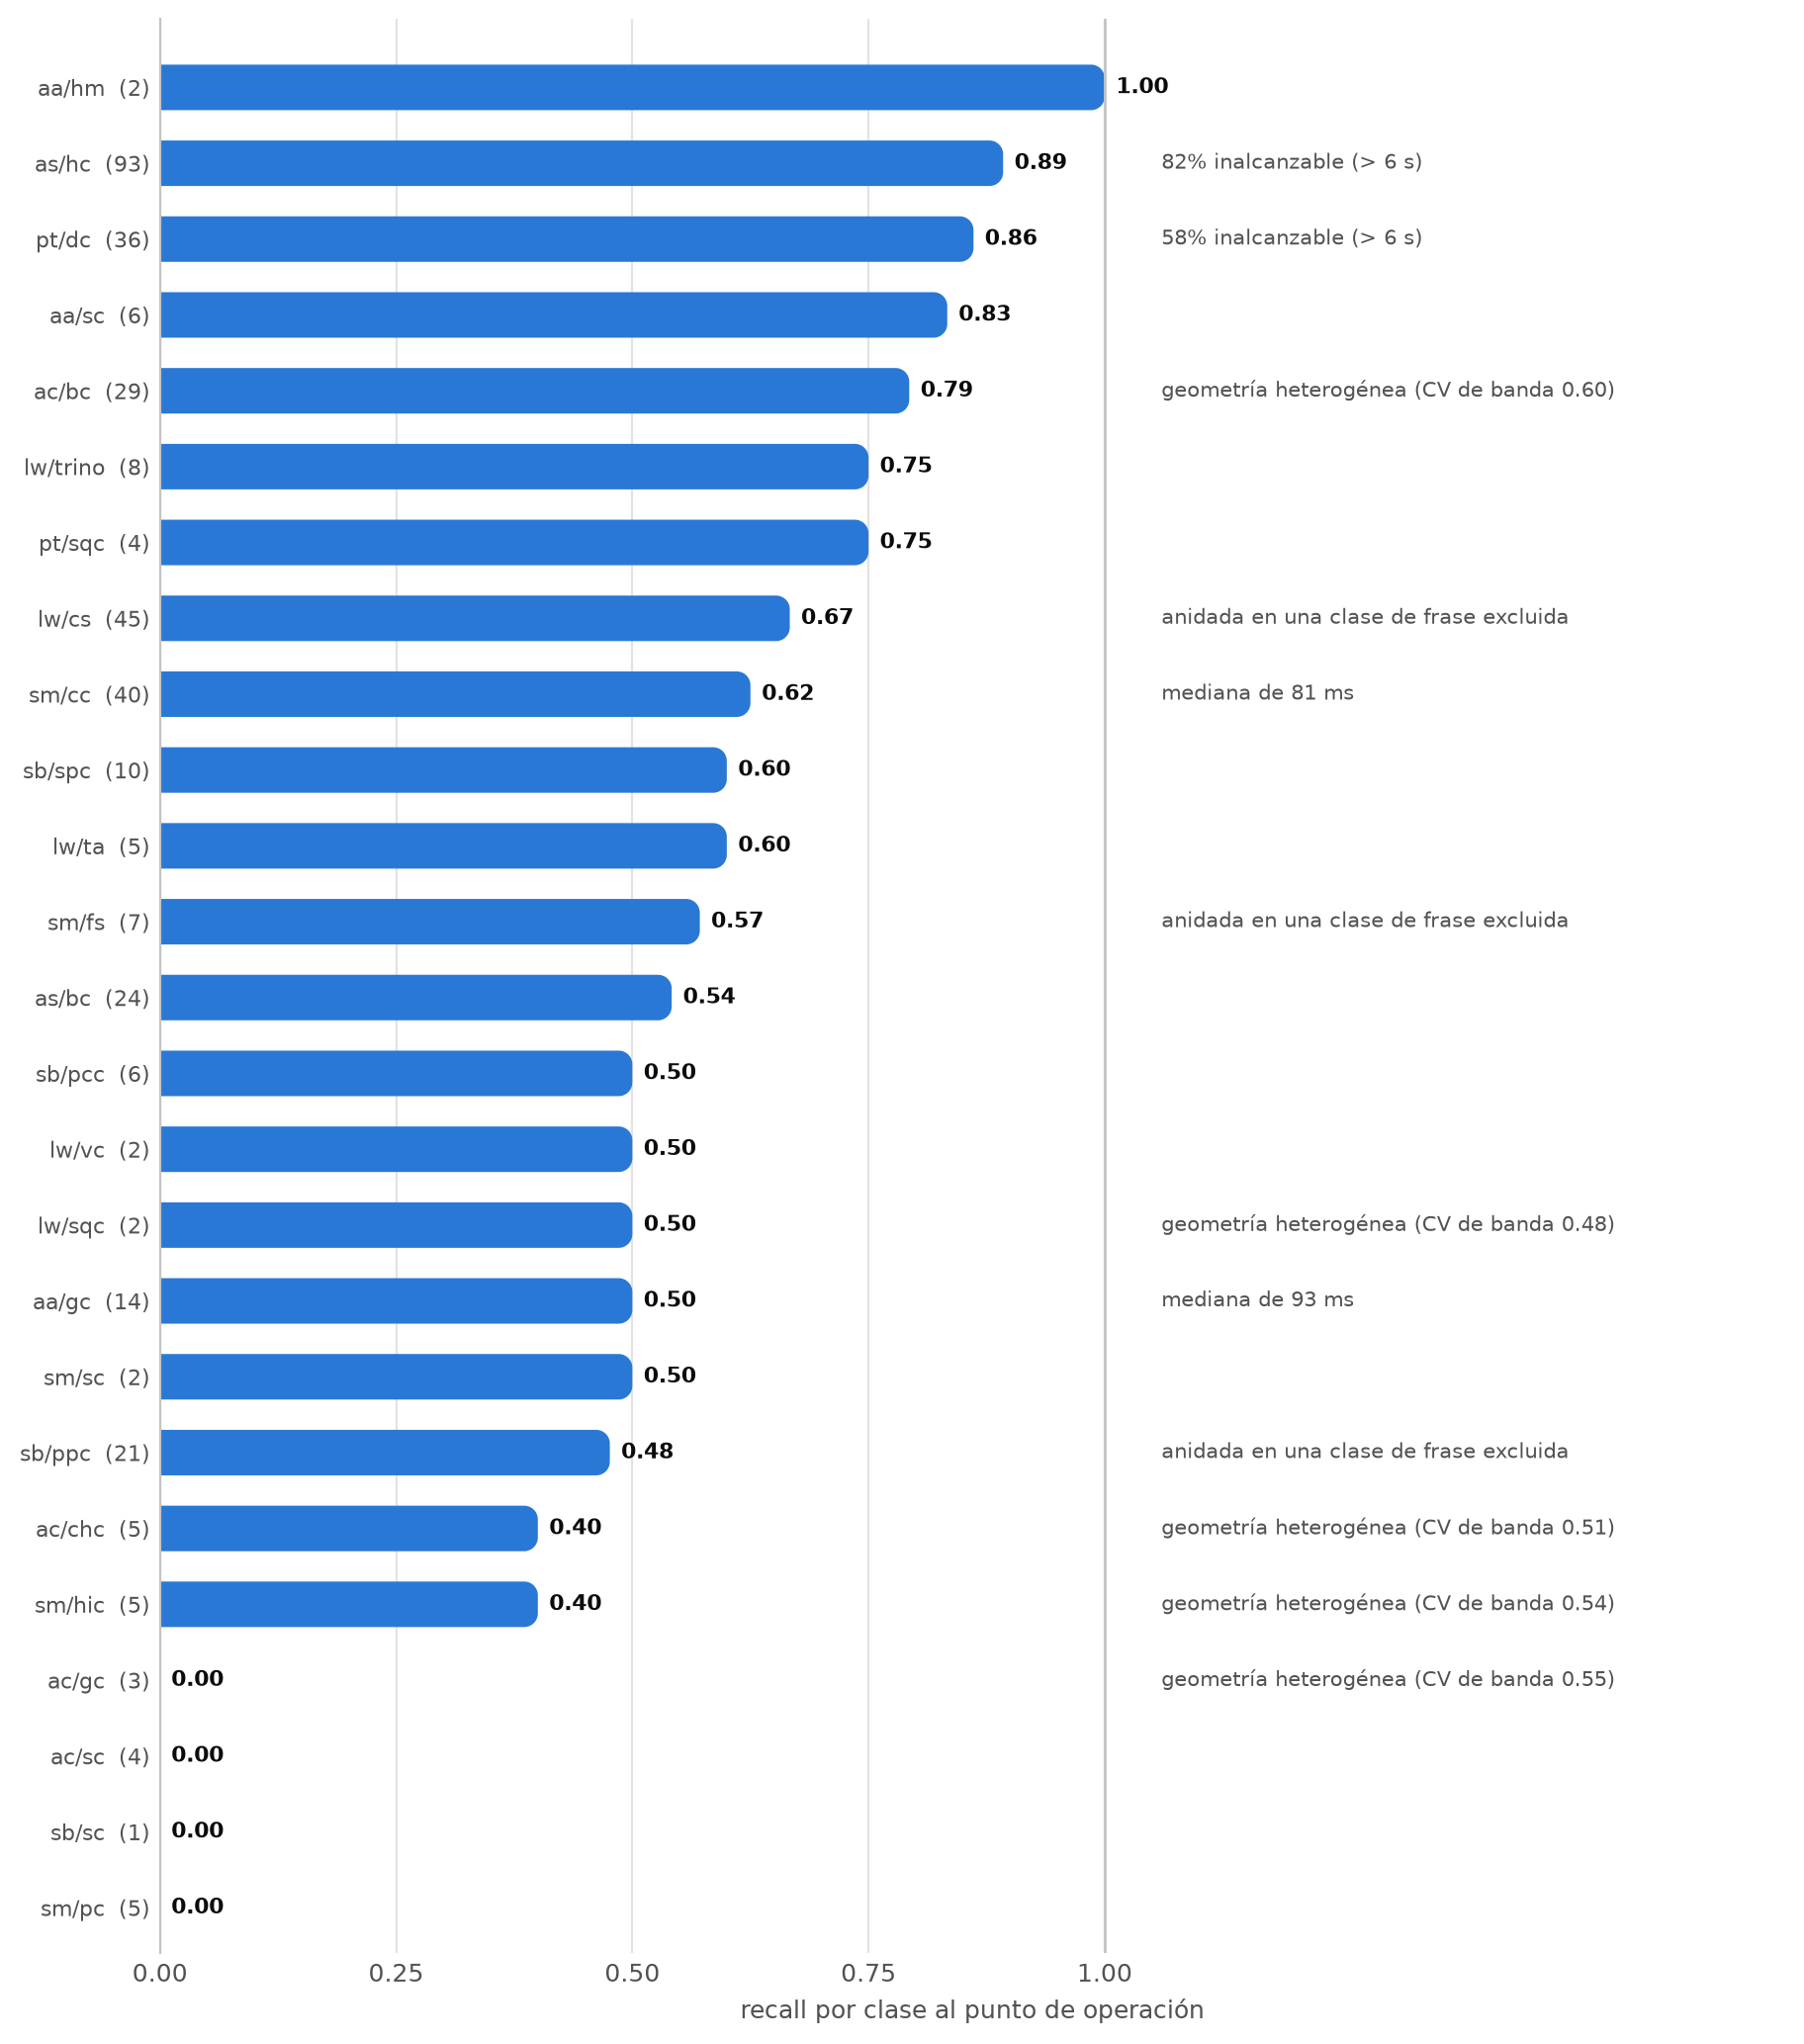
\includegraphics[width=\textwidth]{figures/recall_per_class.png}
%     \caption{Recall por clase.}
%     \label{fig:recall-per-class}
% \end{figure}

\begin{figure}[htbp]
    \centering
    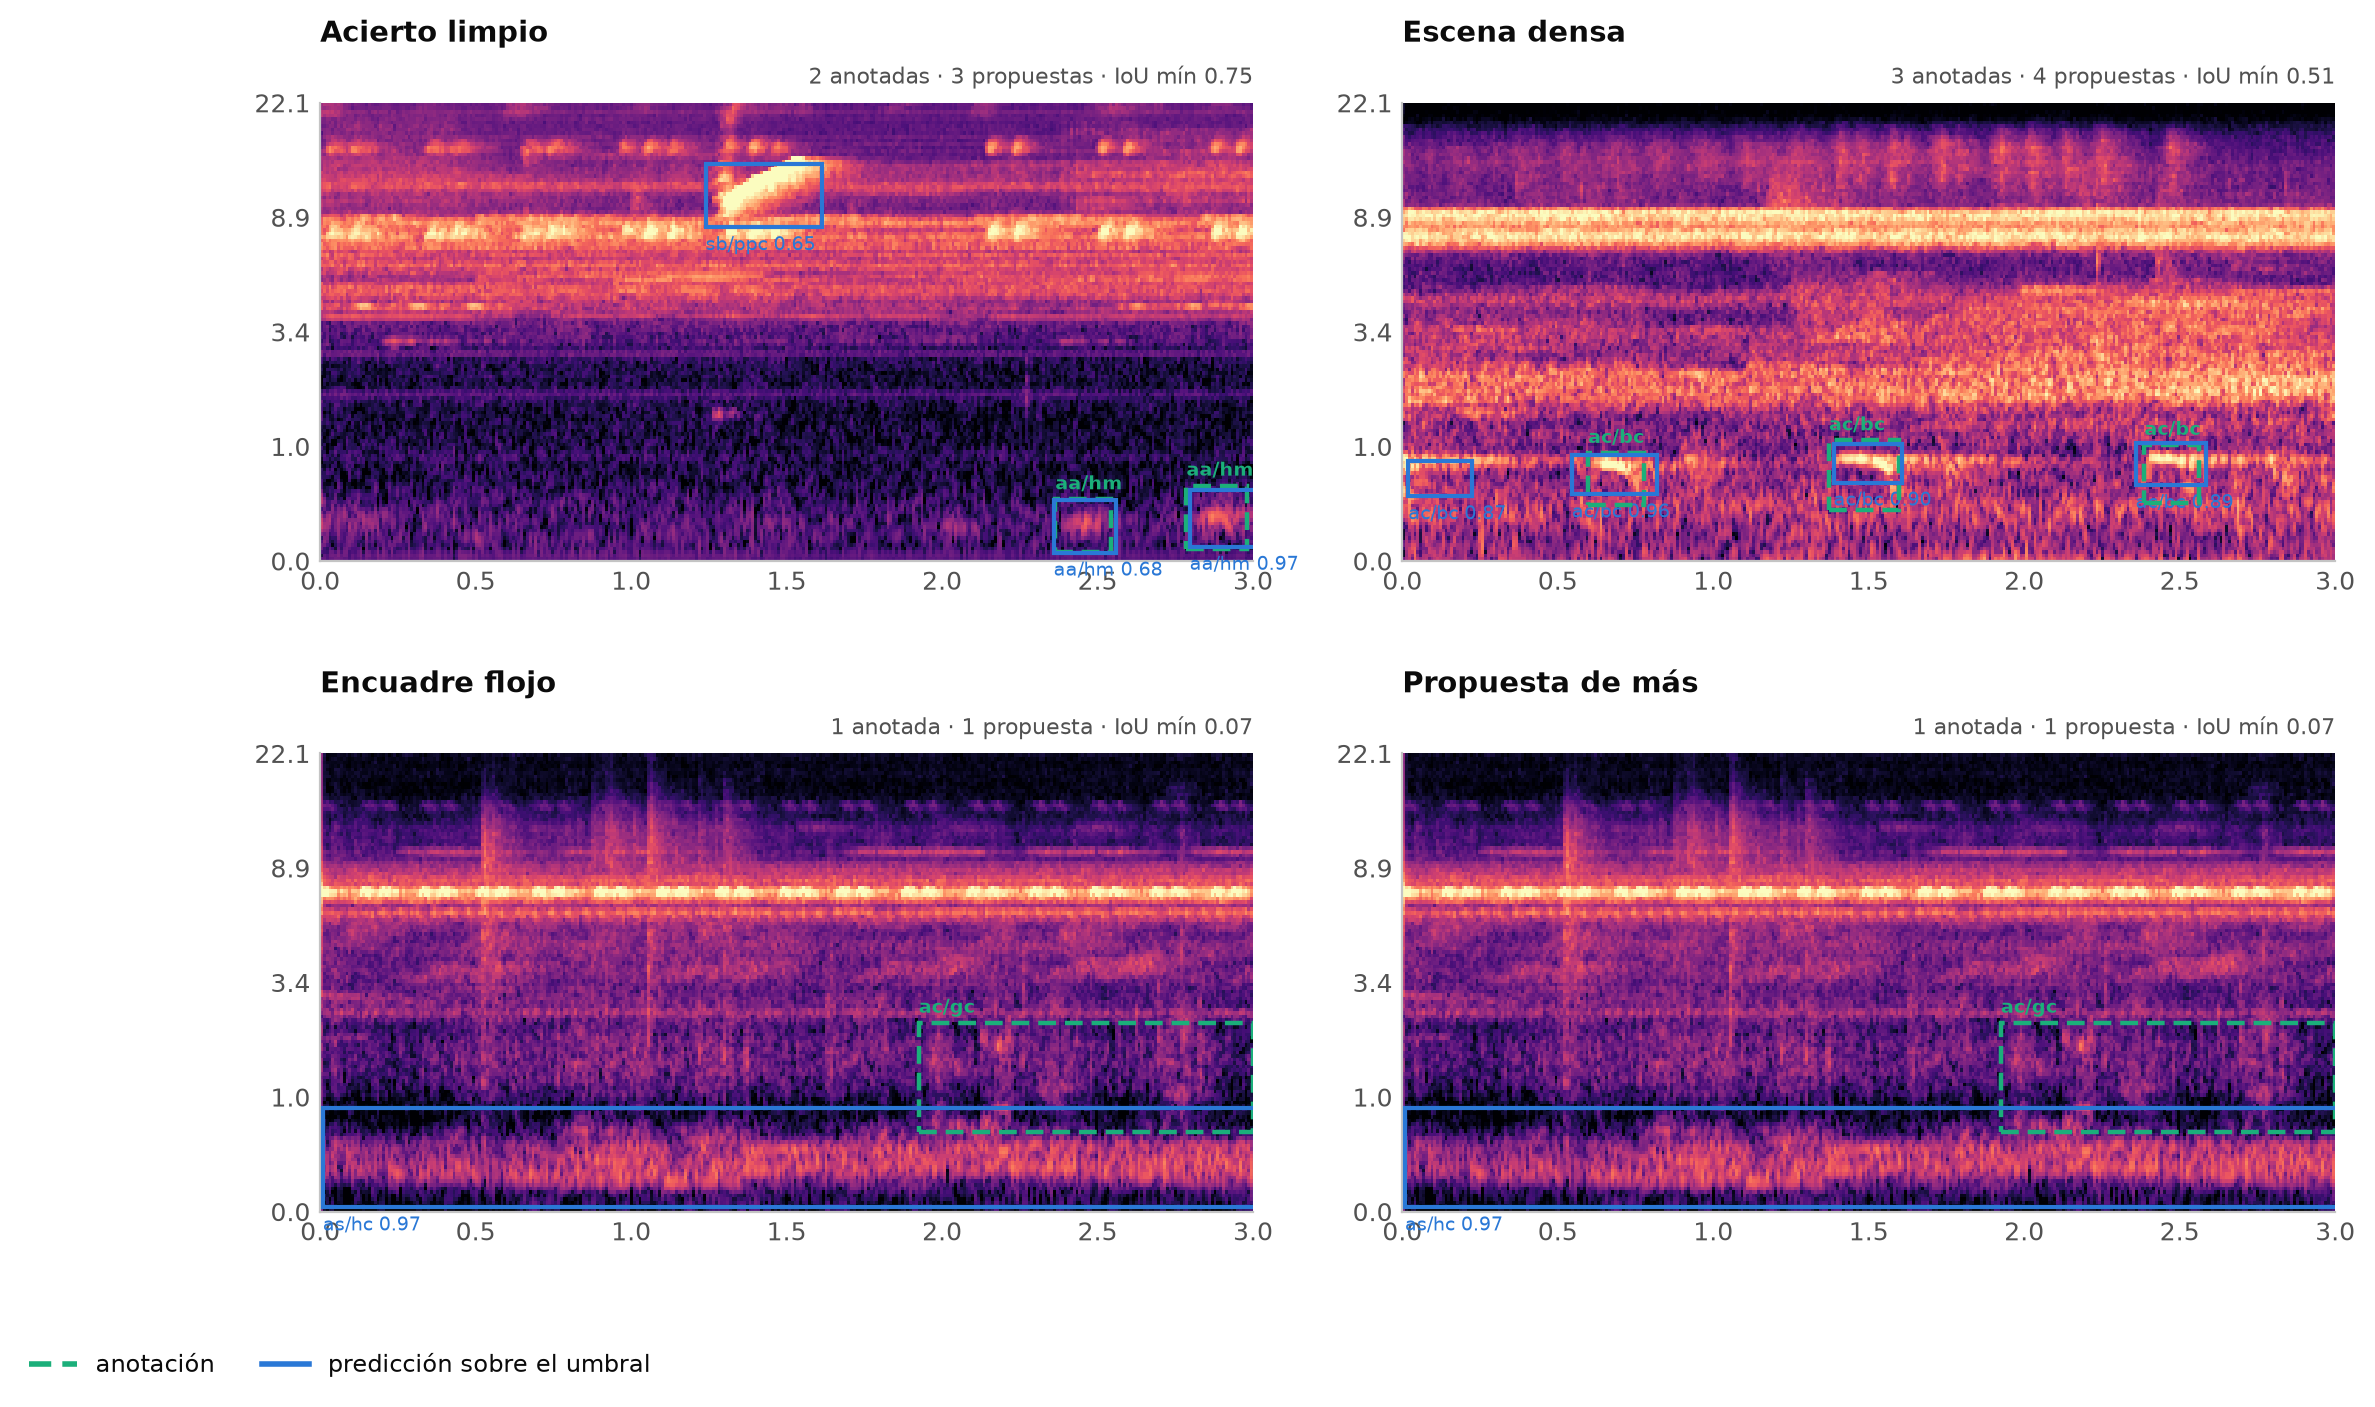
\includegraphics[width=\textwidth]{figures/qualitative_detections.png}
    \caption{Detecciones cualitativas.}
    \label{fig:qualitative-detections}
\end{figure}

\begin{figure}[htbp]
    \centering
    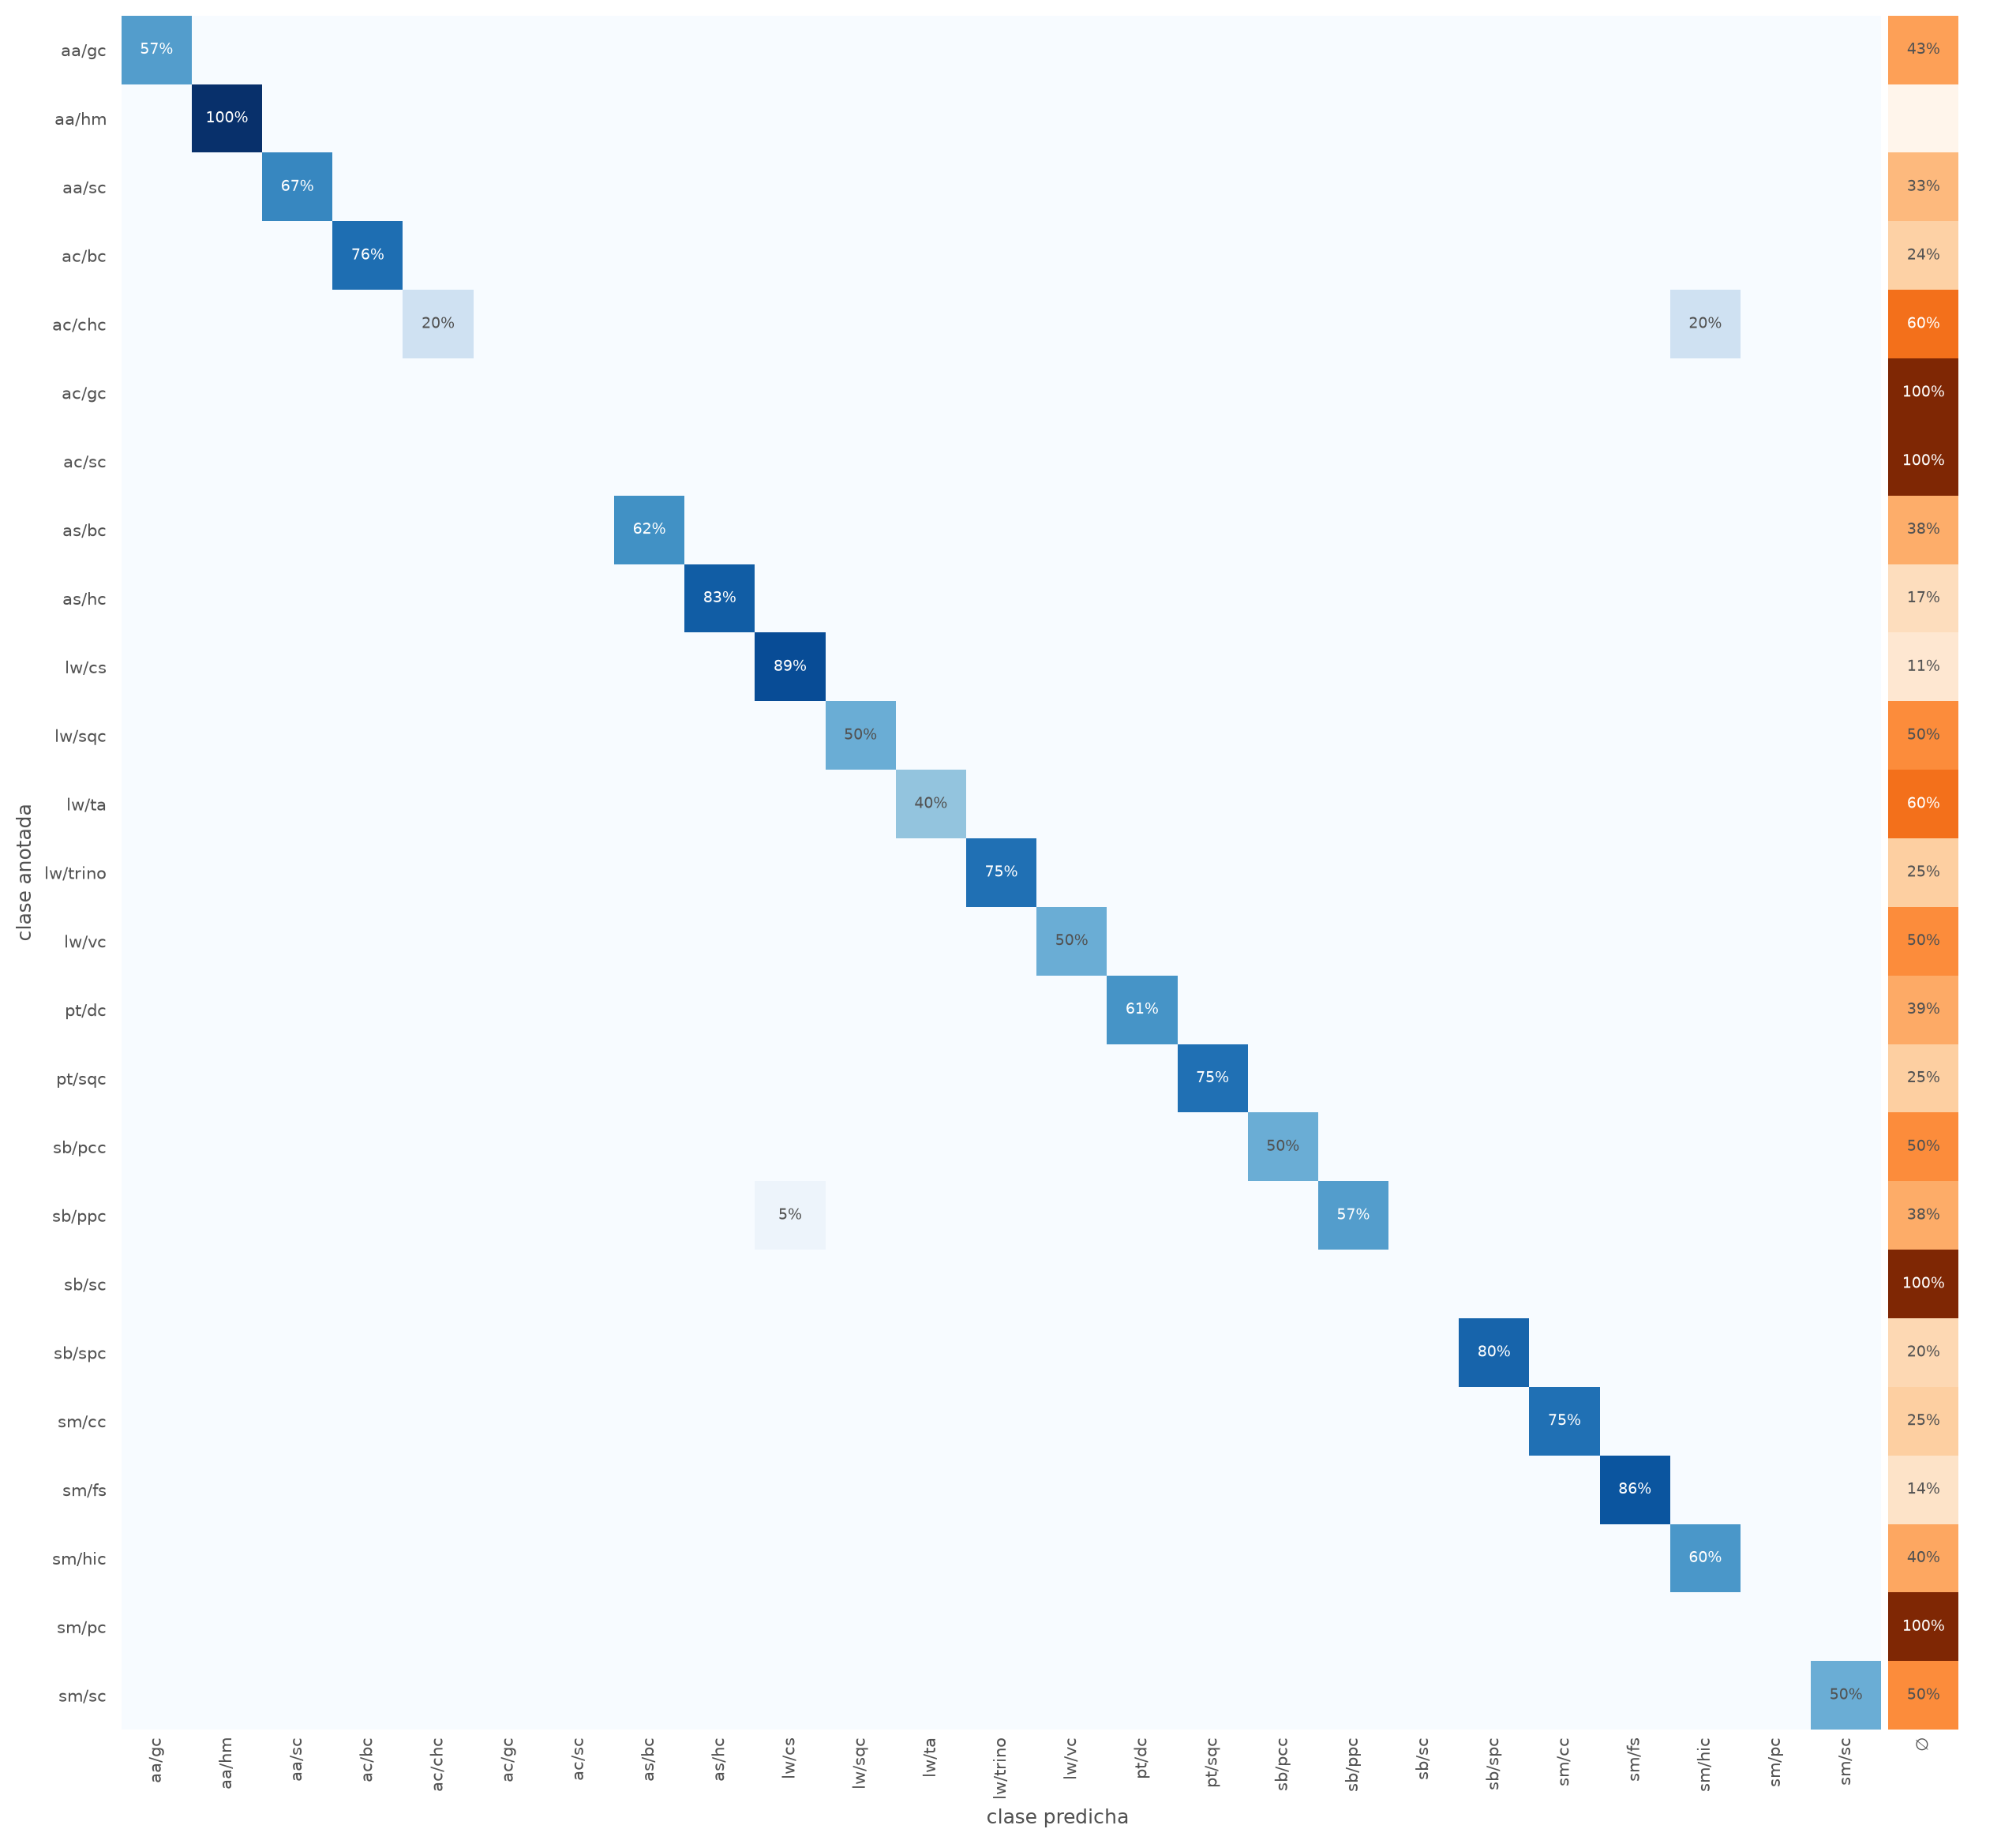
\includegraphics[width=\textwidth]{figures/confusion_matrix.png}
    \caption{Matriz de confusión.}
    \label{fig:confusion-matrix}
\end{figure}

\begin{figure}[htbp]
    \centering
    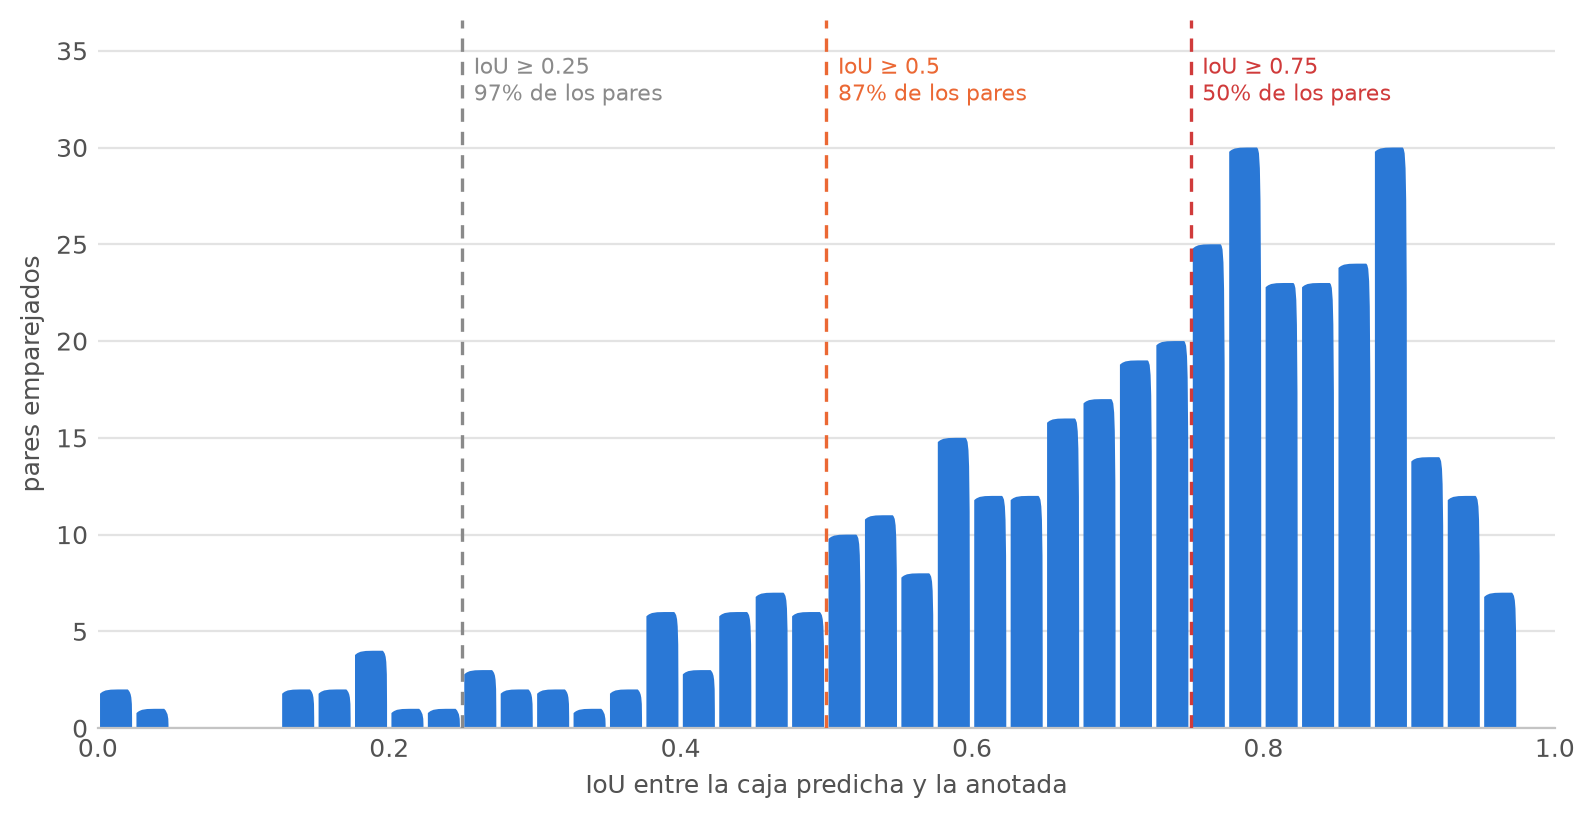
\includegraphics[width=0.9\textwidth]{figures/iou_distribution.png}
    \caption{Distribución de IoU.}
    \label{fig:iou-distribution}
\end{figure}

\begin{figure}[htbp]
    \centering
    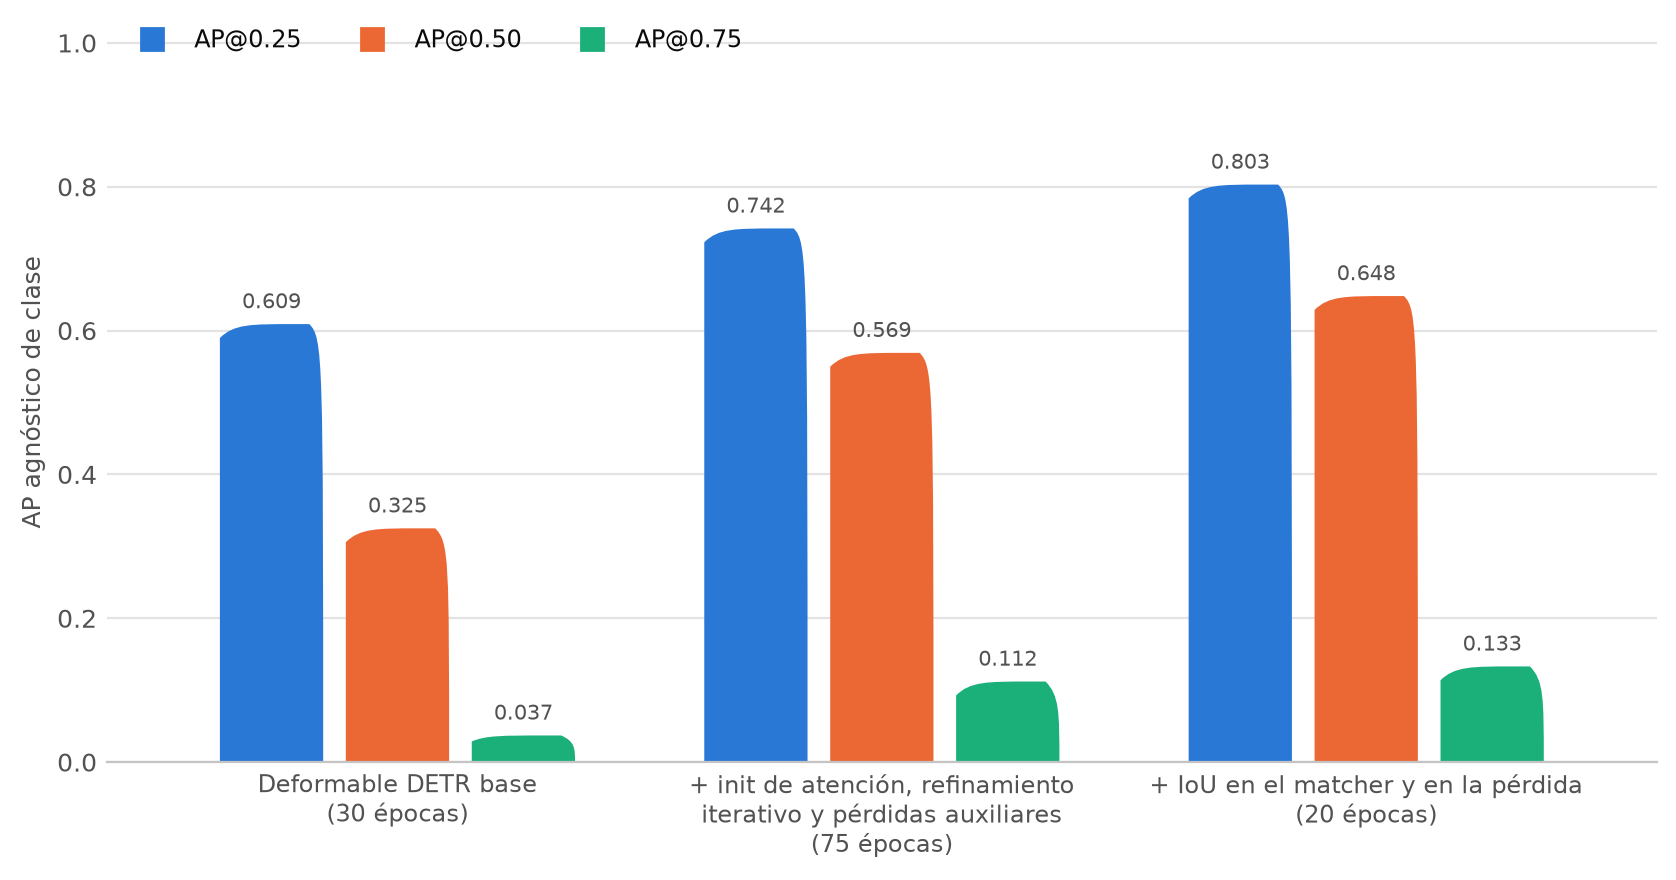
\includegraphics[width=0.92\textwidth]{figures/ablation_progression.png}
    \caption{Ablación acumulada.}
    \label{fig:ablation-progression}
\end{figure}


\section{Exportación a Raven (RE2.4)}
% TODO Redactar.
% TODO FIGURA 5.4: captura de Raven abriendo una tabla de selección
%                  generada por el modelo. Es la prueba visual de que
%                  el sistema cierra el ciclo con el analista.

\begin{figure}[htbp]
    \centering
    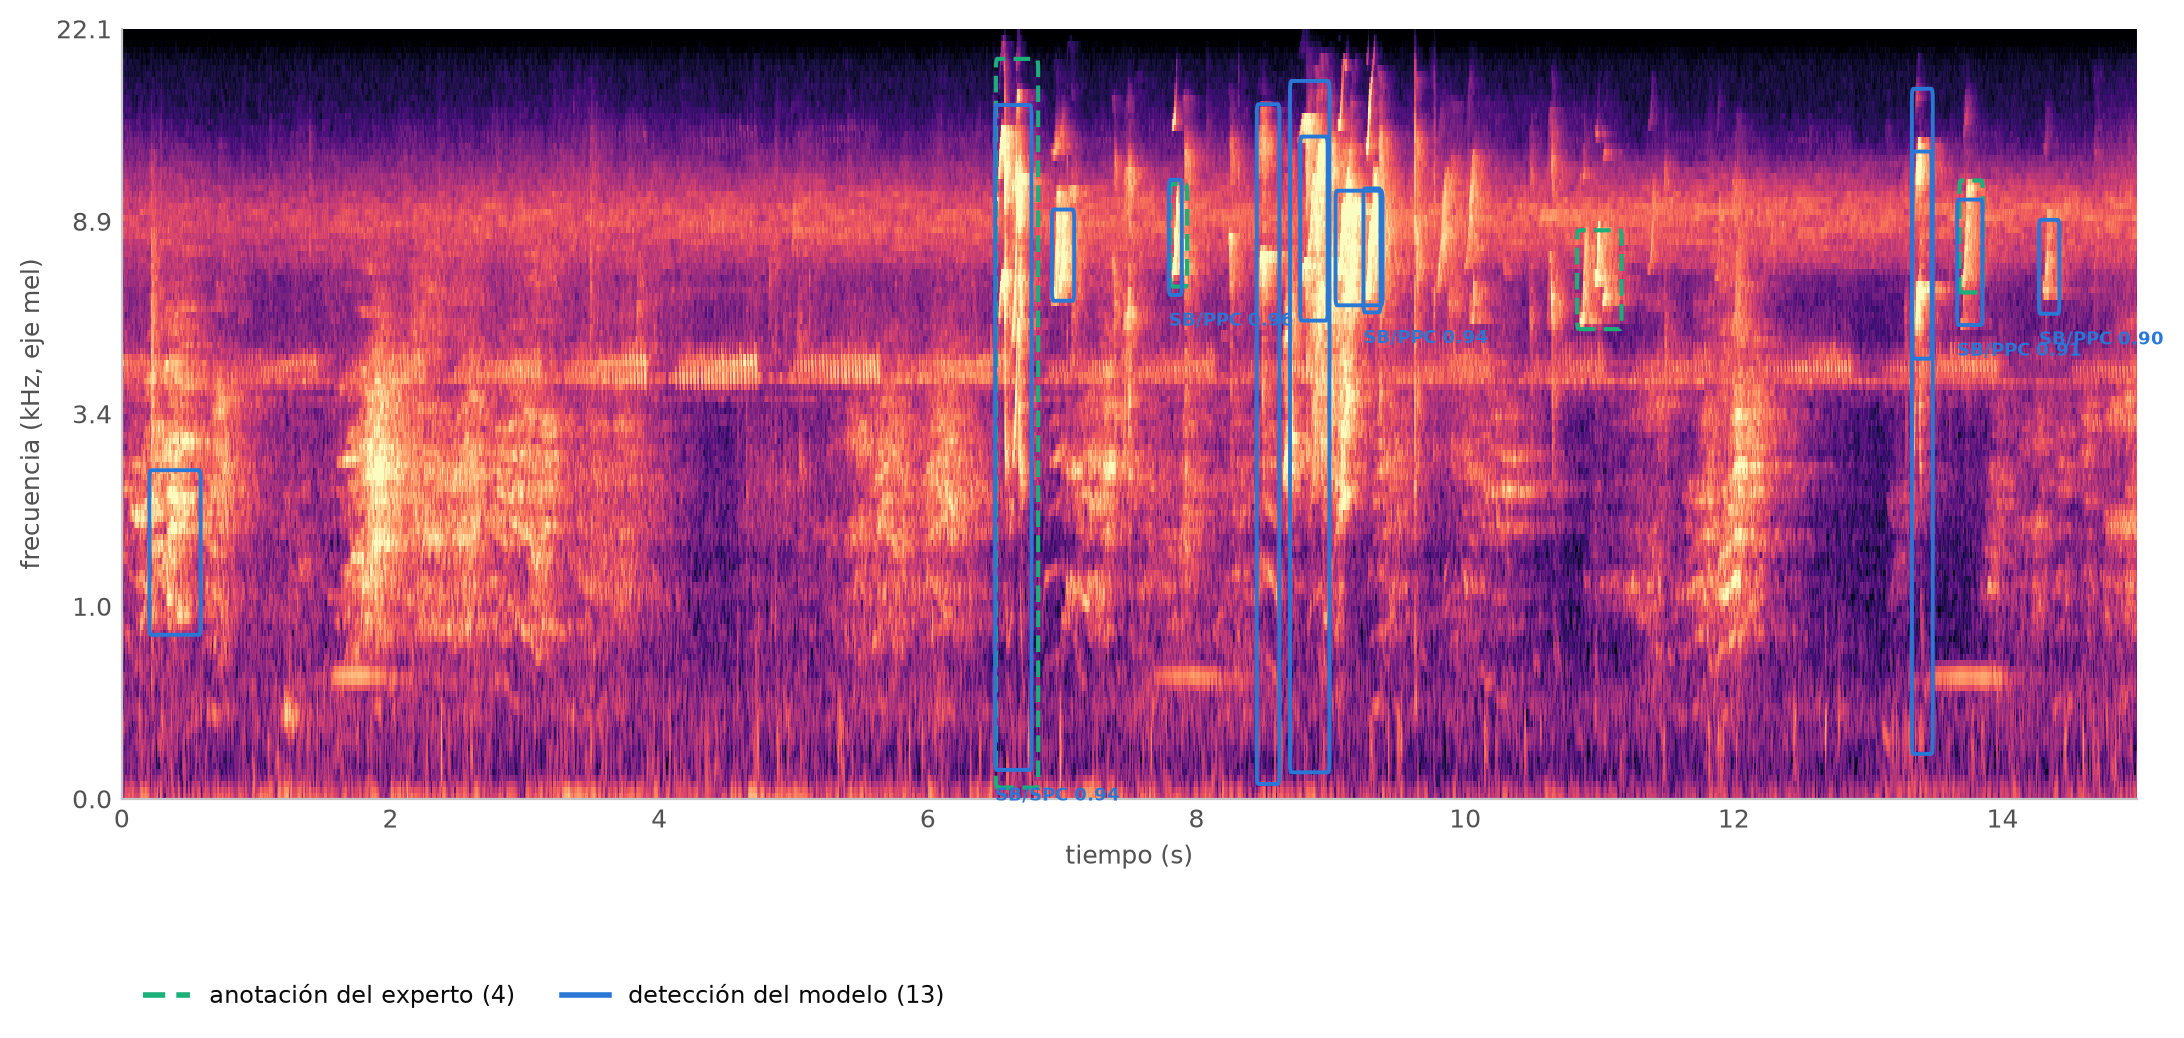
\includegraphics[width=\textwidth]{figures/detection_timeline.png}
    \caption{Línea de tiempo de detecciones.}
    \label{fig:detection-timeline}
\end{figure}

\begin{figure}[htbp]
    \centering
    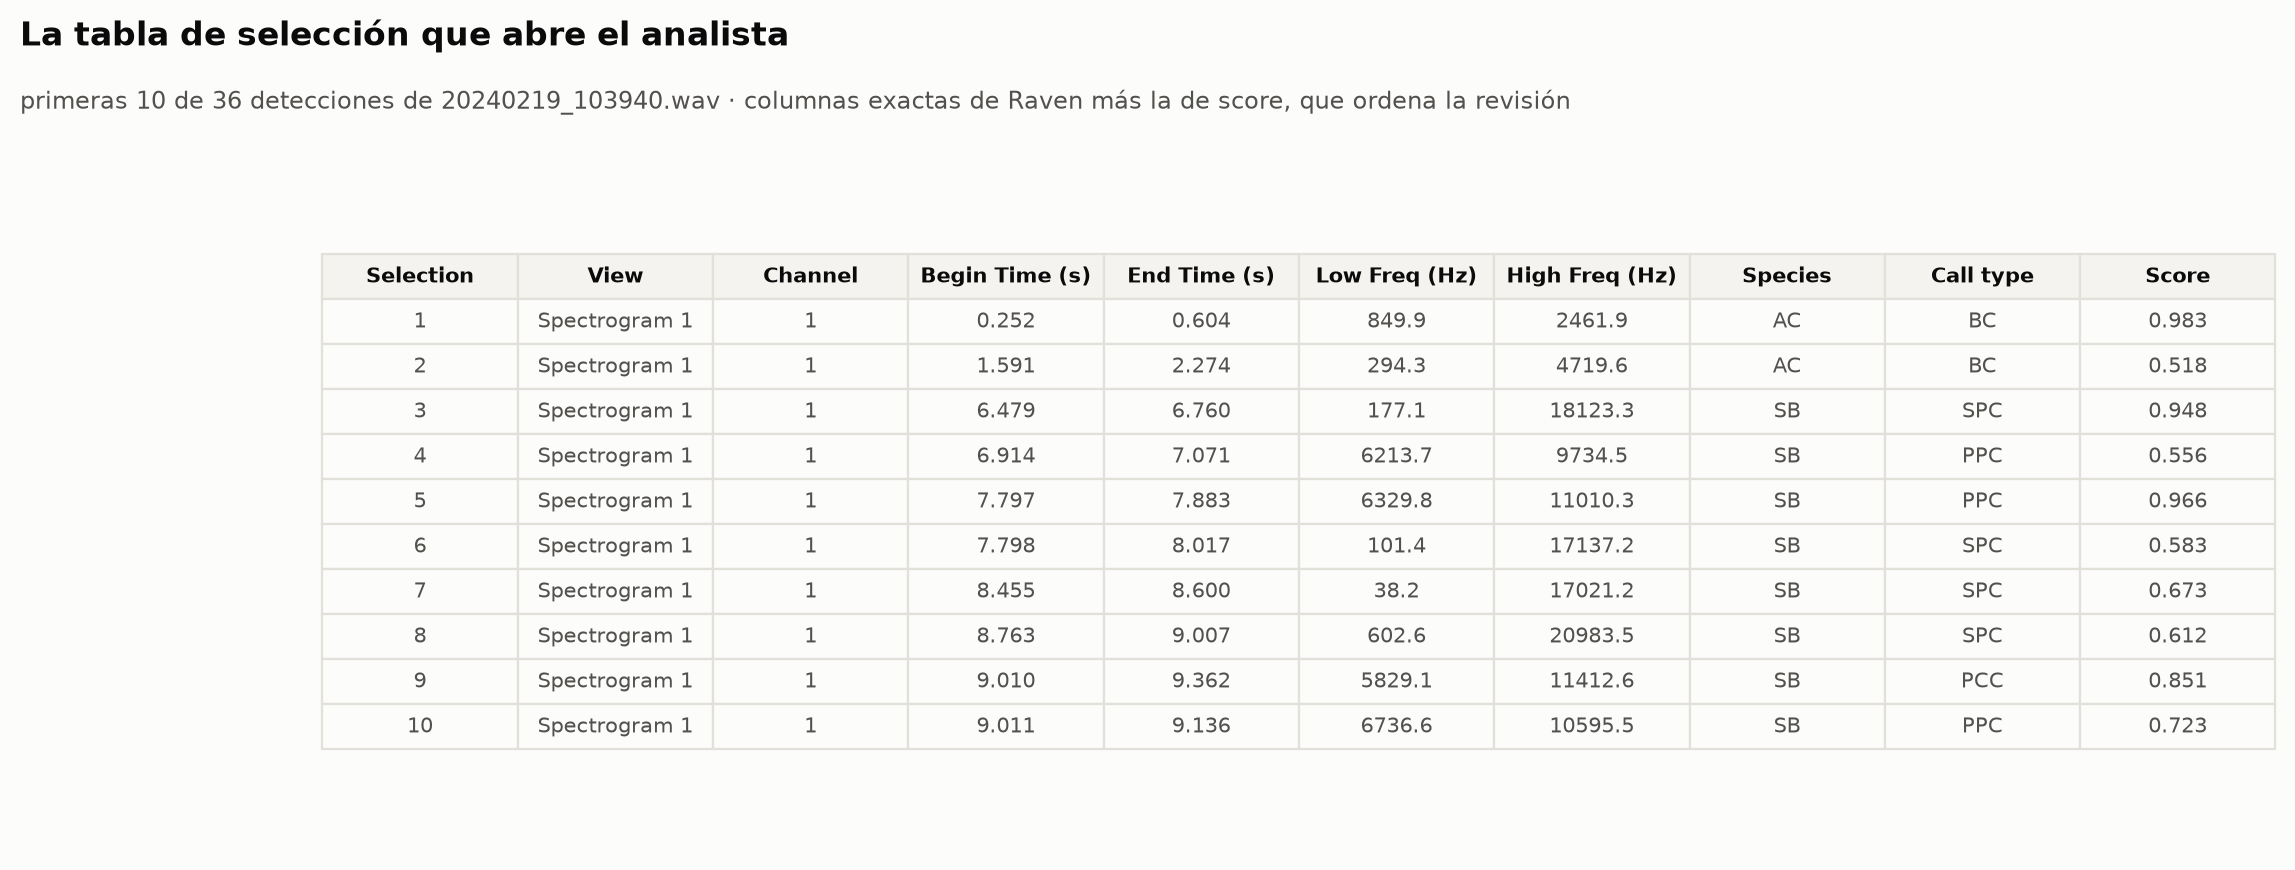
\includegraphics[width=\textwidth]{figures/raven_table_preview.png}
    \caption{Previsualización de la tabla de Raven.}
    \label{fig:raven-table-preview}
\end{figure}

\section{Publicación del código y del modelo (RE2.5)}
% TODO Redactar (breve, media página): URL del repositorio, contenido
% (código del pipeline, pesos del modelo final, instrucciones de
% inferencia), licencia y condiciones de uso. Esta sección faltaba: RE2.5
% se comprometía en el capítulo 1 y en la EDT del anexo, pero ningún
% apartado del cuerpo lo entregaba.

\section{Protocolo de evaluación operativa (RE3.1)}
% TODO Redactar. El protocolo se fecha ANTES de correr la evaluación.
% Debe fijar, en este orden: (1) el subconjunto de prueba, particionado
% por archivo de grabación y sin solapamiento con entrenamiento ni
% validación; (2) el criterio con que se elige el punto de operación
% —umbral que maximiza cobertura sujeto a un techo de propuestas por
% hora—, no un 0,5 heredado; (3) el umbral IoU 0,5 de emparejamiento;
% (4) la supresión de no máximos entre ventanas solapadas de 3 s;
% (5) la agregación de las predicciones por archivo; y (6) las cuatro
% categorías de la Tabla~\ref{tab:taxonomia-fp}.
% ===================================================================

\section{Cobertura frente a carga de revisión (RE3.2)}
% TODO Redactar. Núcleo del capítulo por el lado de OE3.
% TODO FIGURA: curva cobertura (recall por evento @ IoU 0,5) en el eje
%              vertical contra propuestas por hora de audio en el
%              horizontal, con el punto de operación elegido marcado
%              sobre la curva y su criterio anotado.
% TODO TABLA: las cinco magnitudes al punto de operación —cobertura,
%             propuestas por hora, FP/TP, fracción de audio sin
%             ninguna propuesta (reducción de volumen) y minutos de GPU
%             por hora de audio.
% La reducción de volumen es el análogo directo del 22x reportado por
% Campos et al. (2025); citarlo aquí como precedente del indicador.
% Opcional y claramente rotulado como cota ilustrativa: cronometraje de
% una muestra pequeña revisada por el propio autor.
% ===================================================================

\section{Taxonomía de discrepancias (RE3.3)}
% TODO Redactar. Distribuir las predicciones de alta confianza entre
% las categorías A, B, C y D de la Tabla~\ref{tab:taxonomia-fp}.
% TODO TABLA: conteo y porcentaje por categoría.
% TODO FIGURA: distribución de banda de frecuencia, duración y
%              puntuación de las predicciones de tipo D superpuesta a
%              la de los eventos anotados de cada clase.
% TODO FIGURA: panel de espectrogramas con un ejemplo representativo
%              de cada una de las cuatro categorías.
% CUIDADO CON LA REDACCIÓN: el parecido geométrico de las predicciones
% de tipo D con los eventos anotados es INDICIO de omisiones en la
% referencia, no prueba. Usar esa palabra y no otra.
% ===================================================================

\section{Validación experta (RE3.4, condicional)}
% TODO Redactar solo si el equipo de investigación resuelve una muestra
% de predicciones de tipo D. Si no se concreta, esta sección se elimina
% y basta con la limitación ya declarada en el Capítulo~\ref{cap:generalidades}.
% ===================================================================

% ===================================================================
% ANEXOS
% ===================================================================
\appendix
\chapter{Plan del Proyecto}
\label{anx:plan}

\section{Justificación y viabilidad}

\subsection{Justificación}

La investigación es conveniente porque ataca directamente el cuello de botella
descrito en el Capítulo~\ref{cap:generalidades}: el análisis manual del audio
recolectado. El monitoreo acústico pasivo con sensores de bajo costo permite
recolectar a gran escala, pero ese potencial queda desaprovechado mientras el
análisis siga siendo lento, costoso y laborioso. Un sistema de pre-anotación
asistida hace que el monitoreo a gran escala resulte operativamente viable y
permite que el tiempo experto se dedique a la interpretación ecológica en lugar
de al procesamiento.

En el plano práctico, el proyecto reduce la infrautilización del material acústico
acumulado y, con ella, la latencia entre la recolección y la generación de
conocimiento. En el plano teórico, aborda dos vacíos confirmados de forma
independiente por la revisión del Capítulo~\ref{cap:estado}: la ausencia de
modelos y de conjuntos de datos con anotación tiempo--frecuencia para primates
neotropicales, y la falta de estrategias establecidas para el etiquetado
jerárquico de especie y tipo de llamada sobre eventos detectados.

\subsection{Beneficios esperados}

\begin{itemize}[nosep]
    \item Reducir la carga de revisión por hora de audio analizada: menos
          material que inspeccionar para la misma cobertura de eventos.
    \item Poner en uso el audio ya grabado que hoy permanece sin anotar.
    \item Acortar la latencia entre la recolección y la obtención de resultados
          ecológicos.
    \item Disminuir el costo y el error humano asociados al análisis manual.
    \item Entregar una herramienta reutilizable, con código y pesos públicos,
          integrable al flujo de trabajo existente en Raven.
\end{itemize}

\subsection{Viabilidad técnica}

El proyecto no depende de ningún desarrollo previo inexistente. Las
arquitecturas necesarias están disponibles y documentadas
\citep{he_deep_2016,kahl_birdnet_2021,nolasco_learning_2023}; las herramientas
son software libre de uso extendido (Tabla~\ref{tab:herramientas}); los
recursos de cómputo se cubren con acceso a GPU en la nube; los datos iniciales,
aproximadamente 10\,GB de grabaciones WAV capturadas con AudioMoth, con sus
anotaciones de Raven, ya están entregados; y la metodología de trabajo
(CRISP-DM) está establecida y es la que estructura el documento.

\subsection{Viabilidad temporal}

El cronograma es factible dentro del calendario académico, con dos puntos de
tensión identificados. El primero es OE1: la curación y estandarización del
conjunto es meticulosa y cualquier retraso ahí se propaga a todo lo que sigue.
El segundo es OE2, que consume tiempo tanto de cómputo como de análisis humano
en la experimentación. Juega a favor que no haya recolección de datos en campo:
el material de partida ya existe.

\subsection{Viabilidad económica}

El grueso del software es de código abierto y sin costo. Los sensores ya están
desplegados y su costo no recae sobre este proyecto. El desembolso real se
concentra en cómputo en la nube y en servicios de almacenamiento; el resto del
presupuesto es una valorización del tiempo dedicado, no un pago efectivo.

\section{Definición y alcance del proyecto}

\subsection{Alcance}

El proyecto desarrolla y evalúa un sistema de pre-anotación asistida que produce
cajas tiempo--frecuencia etiquetadas sobre grabaciones de monitoreo acústico
pasivo, para las ocho especies de la Tabla~\ref{tab:especies}. El sistema debe
cumplir tres tareas: localizar el evento en tiempo y frecuencia, identificar la
especie y clasificar el tipo de vocalización. Una parte central del alcance es
la caracterización cuantitativa de su comportamiento operativo: la cobertura que
alcanza sobre un conjunto de prueba independiente, la carga de revisión asociada
y la naturaleza de sus discrepancias. Queda fuera del alcance la medición
cronometrada del tiempo de un revisor experto, que depende de la disponibilidad
del equipo de investigación y se declara como resultado condicional. El proyecto
recorre el ciclo completo de CRISP-DM, desde la preparación de los datos hasta el
procesamiento de grabaciones nuevas.

\subsection{Entregables y criterios de aceptación}

Los entregables son los resultados esperados enumerados en la
sección~\ref{sec:resultados}. La Tabla~\ref{tab:aceptacion} recoge el criterio
de aceptación de cada uno: la condición verificable que permite declararlo
terminado.

\begin{table}[htbp]
    \centering
    \caption{Criterios de aceptación}
    \label{tab:aceptacion}
    \small
    \begin{tabular}{@{}L{1.5cm}L{12.9cm}@{}}
        \toprule
        \textbf{Entreg.} & \textbf{Criterio de aceptación}                                                                                                                                                                                  \\
        \midrule
        RE1.1            & El protocolo define reglas de sintaxis para las etiquetas de especie y tipo de llamada, y especifica el tratamiento de errores, duplicados e inconsistencias de las anotaciones originales.                      \\
        \addlinespace
        RE1.2            & Todas las anotaciones del conjunto final cumplen las reglas de RE1.1, y se entrega un manifiesto con la asignación de cada archivo de grabación a una partición.                                                 \\
        \addlinespace
        RE1.3            & La ficha describe la estructura de directorios, incluye un diccionario de datos por columna y declara transformaciones, sesgos y limitaciones conocidas.                                                         \\
        \addlinespace
        RE2.1            & El documento justifica la arquitectura propuesta y la línea base a partir del estado del arte, y fija la configuración e hiperparámetros iniciales de ambas.                                                     \\
        \addlinespace
        RE2.2            & El \textit{pipeline} ejecuta el ciclo completo de entrenamiento, evaluación e inferencia, e incluye instrucciones de instalación y ejecución.                                                                    \\
        \addlinespace
        RE2.3            & El informe presenta las métricas de los tres ejes para la propuesta y la línea base, discute los resultados y concluye con una recomendación justificada.                                                        \\
        \addlinespace
        RE2.4            & Los pesos del modelo se cargan sin error y un script de demostración produce predicciones en el formato de tabla de selección de Raven sobre un clip de prueba.                                                  \\
        \addlinespace
        RE2.5            & El repositorio público contiene el código del \textit{pipeline}, los pesos del modelo final y las instrucciones para reproducir la inferencia.                                                                   \\
        \addlinespace
        RE3.1            & El protocolo, fechado antes de la evaluación, especifica el material de prueba, el criterio de elección del punto de operación, el umbral de IoU que define un verdadero positivo, la agregación por archivo y las cuatro categorías de discrepancia. \\
        \addlinespace
        RE3.2            & Se reporta la curva de cobertura frente a propuestas por hora de audio, el punto de operación elegido con su criterio, el cociente FP/TP, la fracción de audio sin propuestas y el costo de inferencia por hora de audio.                          \\
        \addlinespace
        RE3.3            & El informe distribuye la muestra de predicciones de alta confianza entre las cuatro categorías, caracteriza la categoría D por banda, duración y puntuación frente a los eventos anotados, e incluye ejemplos sobre el espectrograma.                \\
        \addlinespace
        RE3.4            & \textit{Condicional.} Si el equipo de investigación está disponible, se resuelve una muestra de categoría D entre evento omitido y falso positivo genuino y se estima el acuerdo con el criterio experto; si no, la limitación queda declarada.       \\
        \bottomrule
    \end{tabular}
\end{table}

\subsection{Exclusiones}

\begin{itemize}[nosep]
    \item No se desarrolla un sistema de monitoreo en tiempo real desplegable en
          campo; el alcance es el procesamiento de grabaciones existentes.
    \item El análisis detallado de sonidos antropogénicos queda fuera del foco
          primario, más allá de su detección y categorización general.
    \item El estudio se limita a las ocho especies declaradas.
    \item No se desarrolla hardware de adquisición.
    \item No se realiza nueva recolección de datos en campo.
\end{itemize}

\subsection{Limitaciones y restricciones}

\rotulo{Limitaciones.} La ausencia de conjuntos etiquetados a gran escala para
primates neotropicales obliga a invertir un esfuerzo considerable en OE1, y la
calidad de las anotaciones manuales recibidas es subjetiva y variable. El
entorno acústico amazónico es denso y presenta con frecuencia baja relación
señal-ruido. La variabilidad intraespecífica de las vocalizaciones y su
naturaleza graduada dificultan definir categorías discretas, y las llamadas
superpuestas o de baja intensidad son especialmente difíciles de modelar. Los
sensores de bajo costo añaden variabilidad entre dispositivos. Por último, sin
revisión experta las predicciones de alta confianza situadas en regiones sin
anotación (tipo D de la Tabla~\ref{tab:taxonomia-fp}) no pueden clasificarse de
forma concluyente entre eventos omitidos por la referencia y falsos positivos
genuinos: esta tesis las caracteriza geométricamente y las reporta como una
cantidad acotada, y deja su resolución como trabajo futuro condicionado a la
disponibilidad del equipo de investigación.

\rotulo{Restricciones.} El desarrollo está sujeto al calendario académico. El
proyecto depende del conjunto de datos entregado y de la verificación de su
calidad. El acceso a GPU limita la escala de la experimentación, en particular
la búsqueda exhaustiva de hiperparámetros. El desarrollo, la implementación y la
evaluación recaen sobre el autor, con la supervisión del asesor.

\section{Planificación del proyecto}

\subsection{Estructura de desglose del trabajo}

La estructura de desglose se organiza según las fases de CRISP-DM y los
objetivos específicos. La Tabla~\ref{tab:edt} resume los paquetes de trabajo y
el entregable asociado a cada uno.

\begin{table}[htbp]
    \centering
    \caption{EDT del proyecto}
    \label{tab:edt}
    \small
    \begin{tabular}{@{}L{0.8cm}L{4.4cm}L{6.6cm}L{2.2cm}@{}}
        \toprule
        \textbf{ID} & \textbf{Paquete}                 & \textbf{Contenido}                                                                                 & \textbf{Entregable} \\
        \midrule
        1           & Gestión del proyecto             & Planificación, seguimiento, comunicación con el asesor, gestión de riesgos y de la calidad, cierre & N/A                 \\
        \addlinespace
        2           & Comprensión de la investigación  & Objetivos, formulación del problema de detección y criterios de éxito                              & N/A                 \\
        \addlinespace
        3           & Comprensión de los datos         & Acceso al corpus, descripción del formato, análisis exploratorio y verificación de calidad         & N/A                 \\
        \addlinespace
        4.1         & Limpieza y estandarización       & Corrección de etiquetas, tratamiento de audios dañados                                             & RE1.1               \\
        4.2         & Curación del conjunto            & Aplicación del protocolo, vocabulario cerrado, partición por grabación                             & RE1.2               \\
        4.3         & Ingeniería de características    & Preprocesamiento, representación tiempo--frecuencia, ventaneo, aumento de datos                    & N/A                 \\
        4.4         & Documentación del conjunto       & Ficha del conjunto derivado                                                                        & RE1.3               \\
        \addlinespace
        5.1         & Diseño del detector              & Arquitectura propuesta y línea base, con justificación                                             & RE2.1               \\
        5.2         & Implementación                   & \textit{Pipeline} de entrenamiento, evaluación e inferencia                                        & RE2.2               \\
        5.3         & Publicación del código           & Repositorio con código y pesos                                                                     & RE2.5               \\
        \addlinespace
        6.1         & Evaluación cuantitativa          & Métricas por eje, comparación con la línea base, análisis de errores                               & RE2.3               \\
        6.2         & Selección del modelo final       & Modelo elegido y exportador a tabla de selección de Raven                                          & RE2.4               \\
        6.3         & Protocolo de evaluación operativa & Material, criterio de elección del punto de operación, emparejamiento y taxonomía                 & RE3.1               \\
        6.4         & Curva de cobertura y carga       & Barrido de umbral, elección del punto de operación y métricas de carga e inferencia                & RE3.2               \\
        6.5         & Análisis de discrepancias        & Clasificación geométrica de las predicciones de alta confianza y caracterización de la categoría D & RE3.3               \\
        6.6         & Validación experta (condicional) & Revisión de una muestra de categoría D con el equipo de investigación                              & RE3.4               \\
        \addlinespace
        7           & Despliegue                       & Inferencia por lotes sobre grabaciones no vistas y generación de tablas de anotación               & N/A                 \\
        \addlinespace
        8           & Documentación y difusión         & Redacción de la tesis y preparación de la defensa                                                  & N/A                 \\
        \bottomrule
    \end{tabular}
\end{table}

\begin{figure}[htbp]
    \centering
    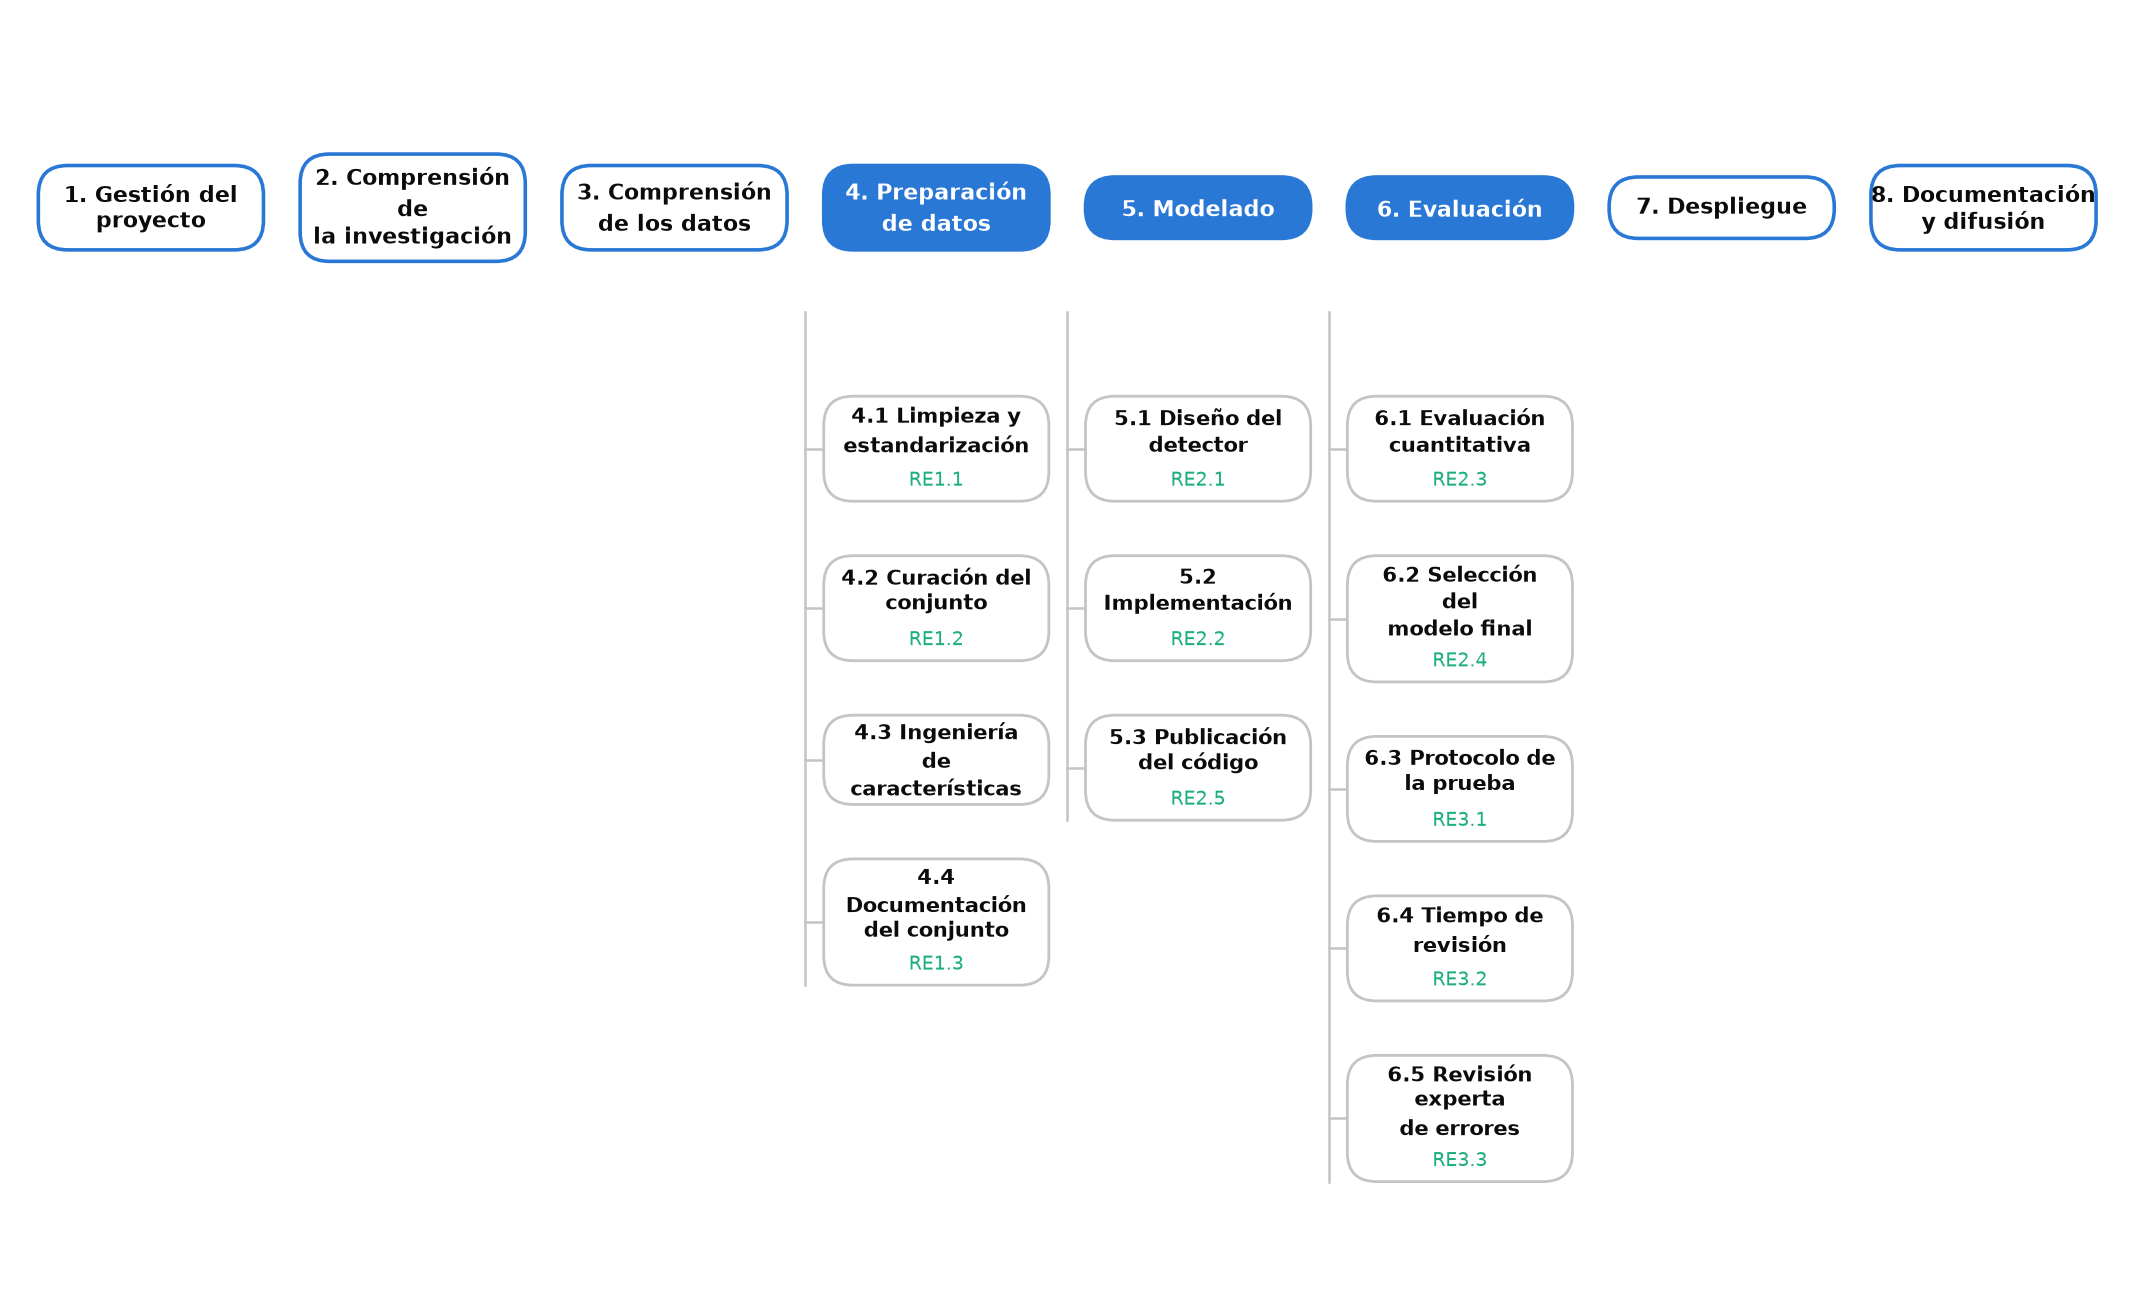
\includegraphics[width=\textwidth]{figures/wbs_tree.png}
    \caption{EDT en árbol.}
    \label{fig:wbs-tree}
\end{figure}

\subsection{Cronograma}

El cronograma se ajusta al calendario académico y se organiza en bloques que
respetan las dependencias entre paquetes: la preparación de datos precede al
modelado, el modelado precede a la evaluación, y el barrido de umbral que produce
la curva de cobertura frente a carga precede al análisis de discrepancias, porque
este se realiza sobre las predicciones del modelo ya seleccionado en el punto de
operación ya elegido. El paquete condicional de validación experta se planifica
al final y fuera de la ruta crítica.


\subsection{Estimación de costos}

Los costos se presentan en dólares estadounidenses y distinguen desembolso real
de valorización. Las Tablas~\ref{tab:costos-hw} a~\ref{tab:costos-ind} detallan
cada categoría, y la Tabla~\ref{tab:costos-resumen} las consolida.

\begin{table}[htbp]
    \centering
    \small
    \begin{threeparttable}
        \caption{Costos de equipos y hardware}
        \label{tab:costos-hw}
        \begin{tabular}{@{}L{4.2cm}L{6.4cm}r@{}}
            \toprule
            \textbf{Categoría}     & \textbf{Descripción}                                               & \thead{USD}        \\
            \midrule
            Almacenamiento externo & SSD de 512\,GB para el conjunto de datos y sus derivados           & 150,00             \\
            \addlinespace
            Equipo de desarrollo   & Laptop con GPU dedicada\tnote{a}                                   & 1\,500,00          \\
            \addlinespace
            Cómputo en la nube     & Instancia con GPU de 48\,GiB de memoria, estimada por horas de uso & 600,00             \\
            \midrule
            \textbf{Subtotal}      &                                                                    & \textbf{2\,250,00} \\
            \bottomrule
        \end{tabular}
        \begin{tablenotes}[flushleft]
            \footnotesize
            \item[a] Equipo preexistente propiedad del tesista. No representa un
            desembolso del proyecto, pero sí un recurso valorizado.
        \end{tablenotes}
    \end{threeparttable}
\end{table}

\begin{table}[htbp]
    \centering
    \small
    \begin{threeparttable}
        \caption[Capital intelectual]{Valorización del capital intelectual}
        \label{tab:costos-rrhh}
        \begin{tabular}{@{}L{5.0cm}rrr@{}}
            \toprule
            \textbf{Recurso}         & \thead{Horas} & \thead{USD/h} & \thead{Total USD}  \\
            \midrule
            Tesista\tnote{a}         & 600           & 5,00          & 2\,500,00          \\
            Asesor de tesis\tnote{b} & 40            & 25,00         & 1\,000,00          \\
            \midrule
            \textbf{Subtotal}        &               &               & \textbf{3\,500,00} \\
            \bottomrule
        \end{tabular}
        \begin{tablenotes}[flushleft]
            \footnotesize
            \item[a] Valorización del tiempo dedicado; no implica un pago real.
            \item[b] Cubierto por la institución.
        \end{tablenotes}
    \end{threeparttable}
\end{table}

\begin{table}[htbp]
    \centering
    \caption[Costos de software y servicios]{Costos de software, licencias y servicios en la nube}
    \label{tab:costos-sw}
    \small
    \begin{tabular}{@{}L{5.0cm}L{3.2cm}rrr@{}}
        \toprule
        \textbf{Software o servicio}      & \textbf{Licencia}      & \thead{Meses} & \thead{USD/mes} & \thead{Total USD} \\
        \midrule
        Python, uv, Pandas, NumPy         & Código abierto         & 12            & 0,00            & 0,00              \\
        PyTorch, torchaudio, Transformers & Código abierto         & 12            & 0,00            & 0,00              \\
        Visual Studio Code                & Código abierto         & 12            & 0,00            & 0,00              \\
        Zotero                            & Gratuito               & 12            & 0,00            & 0,00              \\
        Raven Lite                        & Licencia de estudiante & 12            & 0,00            & 0,00              \\
        Entorno de cómputo con GPU        & Suscripción            & 12            & 9,99            & 119,88            \\
        Almacenamiento en la nube         & Suscripción            & 12            & 1,67            & 20,00             \\
        \midrule
        \textbf{Subtotal}                 &                        &               &                 & \textbf{139,88}   \\
        \bottomrule
    \end{tabular}
\end{table}

\begin{table}[htbp]
    \centering
    \caption{Costos indirectos}
    \label{tab:costos-ind}
    \small
    \begin{tabular}{@{}L{5.4cm}L{4.6cm}rr@{}}
        \toprule
        \textbf{Categoría}  & \textbf{Descripción}                           & \thead{Meses} & \thead{Total USD} \\
        \midrule
        Internet            & Conexión para investigación y acceso a la nube & 12            & 480,00            \\
        Electricidad        & Consumo del equipo y periféricos               & 12            & 360,00            \\
        Impresiones y otros & Materiales de estudio e impresiones            & 12            & 120,00            \\
        \midrule
        \textbf{Subtotal}   &                                                &               & \textbf{960,00}   \\
        \bottomrule
    \end{tabular}
\end{table}

\begin{table}[htbp]
    \centering
    \caption{Resumen de costos}
    \label{tab:costos-resumen}
    \small
    \begin{tabular}{@{}L{7.0cm}r@{}}
        \toprule
        \textbf{Categoría}              & \thead{Total USD}  \\
        \midrule
        Equipamiento (hardware)         & 2\,250,00          \\
        Recursos humanos (valorización) & 3\,500,00          \\
        Software y servicios            & 139,88             \\
        Costos indirectos               & 960,00             \\
        \midrule
        \textbf{Total}                  & \textbf{6\,849,88} \\
        \bottomrule
    \end{tabular}
\end{table}

\subsection{Lista de recursos}

\rotulo{Personas.} El tesista, responsable del desarrollo, la implementación y
el análisis; y el asesor, que aporta guía, supervisión y validación experta.

\rotulo{Equipamiento.} Equipo de desarrollo con GPU dedicada, almacenamiento
externo para el conjunto de datos y sus derivados, y acceso a servidores con GPU
para el entrenamiento.

\rotulo{Herramientas.} Las de la Tabla~\ref{tab:herramientas}, más el acceso a
Raven para la validación cualitativa de las predicciones.

\subsection{Gestión de riesgos}

La Tabla~\ref{tab:riesgos} recoge los riesgos identificados con su probabilidad,
impacto, severidad y las acciones previstas.

\begin{table}[htbp]
    \centering
    \caption[Riesgos del proyecto]{Riesgos del proyecto, mitigación y contingencia}
    \label{tab:riesgos}
    \small
    \begin{tabular}{@{}L{2.8cm}ccL{4.4cm}L{4.2cm}@{}}
        \toprule
        \textbf{Riesgo}                                                       & \thead{Prob.} & \thead{Sever.} & \textbf{Mitigación} & \textbf{Contingencia} \\
        \midrule
        R1. Calidad de los datos: anotaciones inconsistentes y audios dañados &
        Baja                                                                  & Media         &
        Validación cruzada de una muestra con el asesor; detección automática de
        archivos corruptos o vacíos                                           &
        Excluir el material bajo umbral mínimo de calidad y documentar la
        inconsistencia como limitación                                                                                                                       \\
        \addlinespace
        R2. Recursos de cómputo insuficientes                                 &
        Baja                                                                  & Media         &
        Espectrogramas precalculados; \textit{pipeline} de datos optimizado;
        planificación de las corridas largas                                  &
        Reducir la complejidad de las configuraciones menos prometedoras;
        acotar la búsqueda de hiperparámetros; parada temprana                                                                                               \\
        \addlinespace
        R3. Baja disponibilidad de revisores expertos para la validación      &
        Media                                                                 & Baja          &
        Ningún resultado comprometido de OE3 depende de un revisor externo; la
        validación experta se declara como RE3.4 condicional y fuera de la ruta
        crítica                                                               &
        Cerrar OE3 con la caracterización geométrica de la categoría D y
        declarar la limitación de forma explícita                                                                                                            \\
        \addlinespace
        R4. Falla del equipo de desarrollo                                    &
        Alta                                                                  & Media         &
        Código, datos y documentos sincronizados en repositorio remoto; entorno
        replicable por archivo de configuración                               &
        Reinstalar el sistema, clonar el repositorio y recrear el entorno desde
        su especificación                                                                                                                                    \\
        \addlinespace
        R5. Incompatibilidad del entorno de ejecución                         &
        Media                                                                 & Media         &
        Requerimientos explícitos y versionados; contenedor de ejecución;
        versiones estables de las bibliotecas clave                           &
        Proveer un entorno preconfigurado listo para ejecutar; migrar a
        versiones compatibles                                                                                                                                \\
        \addlinespace
        R6. Aumento del costo de cómputo en la nube                           &
        Baja                                                                  & Baja          &
        Desarrollo y depuración en recursos locales o gratuitos; uso eficiente
        de la GPU; priorización de experimentos                               &
        Reducir el alcance de la experimentación; solicitar créditos académicos;
        usar recursos de la universidad                                                                                                                      \\
        \addlinespace
        R7. Retrasos por disponibilidad limitada del tesista                  &
        Alta                                                                  & Alta          &
        Cronograma con holgura basado en la EDT; bloques de tiempo protegidos;
        seguimiento semanal del avance                                        &
        Replanificar al detectar la desviación; negociar reducción de alcance
        con el asesor; priorizar la ruta crítica                                                                                                             \\
        \bottomrule
    \end{tabular}
\end{table}


% ===================================================================
% REFERENCIAS BIBLIOGRÁFICAS
% ===================================================================
\bibliographystyle{apalike}
\bibliography{references}

\end{document}
